% Options for packages loaded elsewhere
\PassOptionsToPackage{unicode}{hyperref}
\PassOptionsToPackage{hyphens}{url}
\PassOptionsToPackage{dvipsnames,svgnames,x11names}{xcolor}
%
\documentclass[
]{article}

\usepackage{amsmath,amssymb}
\usepackage{iftex}
\ifPDFTeX
  \usepackage[T1]{fontenc}
  \usepackage[utf8]{inputenc}
  \usepackage{textcomp} % provide euro and other symbols
\else % if luatex or xetex
  \usepackage{unicode-math}
  \defaultfontfeatures{Scale=MatchLowercase}
  \defaultfontfeatures[\rmfamily]{Ligatures=TeX,Scale=1}
\fi
\usepackage{lmodern}
\ifPDFTeX\else  
    % xetex/luatex font selection
\fi
% Use upquote if available, for straight quotes in verbatim environments
\IfFileExists{upquote.sty}{\usepackage{upquote}}{}
\IfFileExists{microtype.sty}{% use microtype if available
  \usepackage[]{microtype}
  \UseMicrotypeSet[protrusion]{basicmath} % disable protrusion for tt fonts
}{}
\makeatletter
\@ifundefined{KOMAClassName}{% if non-KOMA class
  \IfFileExists{parskip.sty}{%
    \usepackage{parskip}
  }{% else
    \setlength{\parindent}{0pt}
    \setlength{\parskip}{6pt plus 2pt minus 1pt}}
}{% if KOMA class
  \KOMAoptions{parskip=half}}
\makeatother
\usepackage{xcolor}
\setlength{\emergencystretch}{3em} % prevent overfull lines
\setcounter{secnumdepth}{5}
% Make \paragraph and \subparagraph free-standing
\makeatletter
\ifx\paragraph\undefined\else
  \let\oldparagraph\paragraph
  \renewcommand{\paragraph}{
    \@ifstar
      \xxxParagraphStar
      \xxxParagraphNoStar
  }
  \newcommand{\xxxParagraphStar}[1]{\oldparagraph*{#1}\mbox{}}
  \newcommand{\xxxParagraphNoStar}[1]{\oldparagraph{#1}\mbox{}}
\fi
\ifx\subparagraph\undefined\else
  \let\oldsubparagraph\subparagraph
  \renewcommand{\subparagraph}{
    \@ifstar
      \xxxSubParagraphStar
      \xxxSubParagraphNoStar
  }
  \newcommand{\xxxSubParagraphStar}[1]{\oldsubparagraph*{#1}\mbox{}}
  \newcommand{\xxxSubParagraphNoStar}[1]{\oldsubparagraph{#1}\mbox{}}
\fi
\makeatother


\providecommand{\tightlist}{%
  \setlength{\itemsep}{0pt}\setlength{\parskip}{0pt}}\usepackage{longtable,booktabs,array}
\usepackage{calc} % for calculating minipage widths
% Correct order of tables after \paragraph or \subparagraph
\usepackage{etoolbox}
\makeatletter
\patchcmd\longtable{\par}{\if@noskipsec\mbox{}\fi\par}{}{}
\makeatother
% Allow footnotes in longtable head/foot
\IfFileExists{footnotehyper.sty}{\usepackage{footnotehyper}}{\usepackage{footnote}}
\makesavenoteenv{longtable}
\usepackage{graphicx}
\makeatletter
\def\maxwidth{\ifdim\Gin@nat@width>\linewidth\linewidth\else\Gin@nat@width\fi}
\def\maxheight{\ifdim\Gin@nat@height>\textheight\textheight\else\Gin@nat@height\fi}
\makeatother
% Scale images if necessary, so that they will not overflow the page
% margins by default, and it is still possible to overwrite the defaults
% using explicit options in \includegraphics[width, height, ...]{}
\setkeys{Gin}{width=\maxwidth,height=\maxheight,keepaspectratio}
% Set default figure placement to htbp
\makeatletter
\def\fps@figure{htbp}
\makeatother

\usepackage{booktabs}
\usepackage{longtable}
\usepackage{array}
\usepackage{multirow}
\usepackage{wrapfig}
\usepackage{float}
\usepackage{colortbl}
\usepackage{pdflscape}
\usepackage{tabu}
\usepackage{threeparttable}
\usepackage{threeparttablex}
\usepackage[normalem]{ulem}
\usepackage{makecell}
\usepackage{xcolor}
\usepackage{booktabs}
\usepackage{longtable}
\usepackage[a4paper, left=0.75in, right=1in, top=1in, bottom=1in]{geometry}
\makeatletter
\@ifpackageloaded{caption}{}{\usepackage{caption}}
\AtBeginDocument{%
\ifdefined\contentsname
  \renewcommand*\contentsname{Table of contents}
\else
  \newcommand\contentsname{Table of contents}
\fi
\ifdefined\listfigurename
  \renewcommand*\listfigurename{List of Figures}
\else
  \newcommand\listfigurename{List of Figures}
\fi
\ifdefined\listtablename
  \renewcommand*\listtablename{List of Tables}
\else
  \newcommand\listtablename{List of Tables}
\fi
\ifdefined\figurename
  \renewcommand*\figurename{Figure}
\else
  \newcommand\figurename{Figure}
\fi
\ifdefined\tablename
  \renewcommand*\tablename{Table}
\else
  \newcommand\tablename{Table}
\fi
}
\@ifpackageloaded{float}{}{\usepackage{float}}
\floatstyle{ruled}
\@ifundefined{c@chapter}{\newfloat{codelisting}{h}{lop}}{\newfloat{codelisting}{h}{lop}[chapter]}
\floatname{codelisting}{Listing}
\newcommand*\listoflistings{\listof{codelisting}{List of Listings}}
\makeatother
\makeatletter
\makeatother
\makeatletter
\@ifpackageloaded{caption}{}{\usepackage{caption}}
\@ifpackageloaded{subcaption}{}{\usepackage{subcaption}}
\makeatother

\ifLuaTeX
  \usepackage{selnolig}  % disable illegal ligatures
\fi
\usepackage{bookmark}

\IfFileExists{xurl.sty}{\usepackage{xurl}}{} % add URL line breaks if available
\urlstyle{same} % disable monospaced font for URLs
\hypersetup{
  pdftitle={DAA Taxa},
  colorlinks=true,
  linkcolor={blue},
  filecolor={Maroon},
  citecolor={Blue},
  urlcolor={Blue},
  pdfcreator={LaTeX via pandoc}}


\title{DAA Taxa}
\author{}
\date{}

\begin{document}
\maketitle


\section{Differential abundance
analysis}\label{differential-abundance-analysis}

Analysis information:

\begin{itemize}
\tightlist
\item
  Method: maaslin3
\item
  Taxonomic level: species, genus, family, phylum
\item
  Group variable: diet
\item
  Formula used: \textbf{\textasciitilde{} diet * intervention + (1
  \textbar{} id)}
\item
  Correction: \textbf{Benjamini-Hochberg FDR adjustment}
\item
  Detection threshold: 0.1\%
\item
  Prevalence threshold: 10\%
\end{itemize}

For a complete table of maaslin3 results, see
\href{https://github.com/openresearchlabs/OGB_project/blob/main/output/daa/daa_taxa/species/all_results.tsv}{Species},
\href{https://github.com/openresearchlabs/OGB_project/blob/main/output/daa/daa_taxa/genus/all_results.tsv}{genus},
\href{https://github.com/openresearchlabs/OGB_project/blob/main/output/daa/daa_taxa/phylum/all_results.tsv}{phylum},
\href{https://github.com/openresearchlabs/OGB_project/blob/main/output/daa/daa_taxa/family/all_results.tsv}{family}

The following tables lists all associations that pass MaAsLin 3's
significance threshold for joint or individual q-values, ordered by
increasing individual q-value.

\begin{longtable}[t]{lrrrrrr}
\caption{Table of significant features for species - Total features analyzed: 215 - Model: abundance}\\
\toprule
\textbf{feature} & \textbf{metadata} & \textbf{value} & \textbf{coef} & \textbf{qval\_individual} & \textbf{qval\_joint} & \textbf{model}\\
\midrule
\endfirsthead
\caption[]{Table of significant features for species - Total features analyzed: 215 - Model: abundance \textit{(continued)}}\\
\toprule
\textbf{feature} & \textbf{metadata} & \textbf{value} & \textbf{coef} & \textbf{qval\_individual} & \textbf{qval\_joint} & \textbf{model}\\
\midrule
\endhead

\endfoot
\bottomrule
\endlastfoot
GGB1266\_SGB1699 & intervention & oat & 4.593 & 0.048 & 0.028 & abundance\\
Waltera\_intestinalis & diet & oat & -3.609 & 0.052 & 0.040 & abundance\\
Dorea\_longicatena & intervention & oat & 1.193 & 0.082 & 0.084 & abundance\\
Dorea\_longicatena & diet & oat & 1.139 & 0.112 & 0.000 & abundance\\
Ruminococcus\_sp\_BSD2780120874\_150323\_B10 & diet & oat & -5.197 & 0.139 & 0.085 & abundance\\
\addlinespace
Dorea\_longicatena & diet & oat:interventionoat & -1.524 & 0.174 & 0.001 & abundance\\
Alistipes\_communis & diet & oat:interventionoat & 1.857 & 0.782 & 0.049 & abundance\\
Firmicutes\_bacterium\_AF16\_15 & intervention & oat & 1.320 & 0.782 & 0.000 & abundance\\
GGB2982\_SGB3964 & diet & oat:interventionoat & 1.287 & 0.782 & 0.046 & abundance\\
Lachnospiraceae\_bacterium & intervention & oat & 1.200 & 0.782 & 0.049 & abundance\\
\addlinespace
Bacteroides\_uniformis & intervention & oat & 0.673 & 0.888 & 0.001 & abundance\\
Firmicutes\_bacterium\_AF16\_15 & diet & oat:interventionoat & -1.413 & 0.958 & 0.048 & abundance\\
Clostridium\_sp\_AF34\_10BH & diet & oat:interventionoat & -1.145 & 0.989 & 0.072 & abundance\\
Adlercreutzia\_equolifaciens & diet & oat:interventionoat & -0.081 & 1.000 & 0.000 & abundance\\
Agathobaculum\_butyriciproducens & diet & oat & 0.264 & 1.000 & 0.000 & abundance\\
\addlinespace
Agathobaculum\_butyriciproducens & diet & oat:interventionoat & -0.168 & 1.000 & 0.048 & abundance\\
Bacteroides\_ovatus & diet & oat:interventionoat & -0.982 & 1.000 & 0.090 & abundance\\
Bacteroides\_ovatus & intervention & oat & 0.872 & 1.000 & 0.001 & abundance\\
Bifidobacterium\_longum & intervention & oat & -0.477 & 1.000 & 0.011 & abundance\\
Clostridium\_sp\_AF34\_10BH & intervention & oat & 0.605 & 1.000 & 0.000 & abundance\\
\addlinespace
Dorea\_sp\_AF36\_15AT & intervention & oat & 0.344 & 1.000 & 0.000 & abundance\\
Dysosmobacter\_welbionis & diet & oat:interventionoat & 0.164 & 1.000 & 0.053 & abundance\\
Dysosmobacter\_welbionis & intervention & oat & 0.162 & 1.000 & 0.000 & abundance\\
Eubacterium\_rectale & diet & oat:interventionoat & -0.889 & 1.000 & 0.000 & abundance\\
Evtepia\_gabavorous & diet & oat:interventionoat & -0.564 & 1.000 & 0.047 & abundance\\
\addlinespace
Evtepia\_gabavorous & intervention & oat & 0.090 & 1.000 & 0.085 & abundance\\
Faecalibacillus\_faecis & diet & oat:interventionoat & -0.700 & 1.000 & 0.014 & abundance\\
Faecalibacillus\_faecis & intervention & oat & 0.011 & 1.000 & 0.001 & abundance\\
Flavonifractor\_plautii & diet & oat:interventionoat & 1.103 & 1.000 & 0.000 & abundance\\
Flavonifractor\_plautii & intervention & oat & -0.368 & 1.000 & 0.000 & abundance\\
\addlinespace
GGB33469\_SGB15236 & diet & oat & -0.753 & 1.000 & 0.085 & abundance\\
GGB79734\_SGB15291 & diet & oat:interventionoat & 0.316 & 1.000 & 0.047 & abundance\\
GGB9760\_SGB15373 & diet & oat:interventionoat & -0.621 & 1.000 & 0.047 & abundance\\
Parabacteroides\_merdae & diet & oat:interventionoat & -1.082 & 1.000 & 0.047 & abundance\\
Phascolarctobacterium\_faecium & diet & oat & -0.787 & 1.000 & 0.011 & abundance\\
\addlinespace
Ruminococcus\_torques & diet & oat:interventionoat & -0.960 & 1.000 & 0.000 & abundance\\*
\end{longtable}

\begin{longtable}[t]{lrrrrrr}
\caption{Table of significant features for species - Total features analyzed: 215 - Model: prevalence}\\
\toprule
\textbf{feature} & \textbf{metadata} & \textbf{value} & \textbf{coef} & \textbf{qval\_individual} & \textbf{qval\_joint} & \textbf{model}\\
\midrule
\endfirsthead
\caption[]{Table of significant features for species - Total features analyzed: 215 - Model: prevalence \textit{(continued)}}\\
\toprule
\textbf{feature} & \textbf{metadata} & \textbf{value} & \textbf{coef} & \textbf{qval\_individual} & \textbf{qval\_joint} & \textbf{model}\\
\midrule
\endhead

\endfoot
\bottomrule
\endlastfoot
Dorea\_longicatena & diet & oat & 11.199 & 0.000 & 0.000 & prevalence\\
Ruminococcus\_torques & diet & oat:interventionoat & 11.154 & 0.000 & 0.000 & prevalence\\
Firmicutes\_bacterium\_AF16\_15 & intervention & oat & 11.584 & 0.000 & 0.000 & prevalence\\
Agathobaculum\_butyriciproducens & diet & oat & 9.751 & 0.000 & 0.000 & prevalence\\
Dorea\_sp\_AF36\_15AT & intervention & oat & 9.327 & 0.000 & 0.000 & prevalence\\
\addlinespace
Flavonifractor\_plautii & intervention & oat & 11.272 & 0.000 & 0.000 & prevalence\\
Eubacterium\_rectale & diet & oat:interventionoat & 8.883 & 0.000 & 0.000 & prevalence\\
Dysosmobacter\_welbionis & intervention & oat & 12.382 & 0.000 & 0.000 & prevalence\\
Adlercreutzia\_equolifaciens & diet & oat:interventionoat & 8.288 & 0.000 & 0.000 & prevalence\\
Clostridium\_sp\_AF34\_10BH & intervention & oat & 9.732 & 0.000 & 0.000 & prevalence\\
\addlinespace
Flavonifractor\_plautii & diet & oat:interventionoat & -11.754 & 0.000 & 0.000 & prevalence\\
Bacteroides\_ovatus & intervention & oat & 8.632 & 0.001 & 0.001 & prevalence\\
Bacteroides\_uniformis & intervention & oat & 8.204 & 0.001 & 0.001 & prevalence\\
Dorea\_longicatena & diet & oat:interventionoat & -12.474 & 0.001 & 0.001 & prevalence\\
Faecalibacillus\_faecis & intervention & oat & 18.357 & 0.001 & 0.001 & prevalence\\
\addlinespace
Bifidobacterium\_longum & intervention & oat & 7.617 & 0.011 & 0.011 & prevalence\\
Phascolarctobacterium\_faecium & diet & oat & 15.101 & 0.011 & 0.011 & prevalence\\
Faecalibacillus\_faecis & diet & oat:interventionoat & -17.732 & 0.013 & 0.014 & prevalence\\
Evtepia\_gabavorous & diet & oat:interventionoat & -17.953 & 0.048 & 0.047 & prevalence\\
GGB2982\_SGB3964 & diet & oat:interventionoat & -18.105 & 0.048 & 0.046 & prevalence\\
\addlinespace
GGB79734\_SGB15291 & diet & oat:interventionoat & -16.488 & 0.048 & 0.047 & prevalence\\
GGB9760\_SGB15373 & diet & oat:interventionoat & -18.061 & 0.048 & 0.047 & prevalence\\
Parabacteroides\_merdae & diet & oat:interventionoat & -17.142 & 0.048 & 0.047 & prevalence\\
Firmicutes\_bacterium\_AF16\_15 & diet & oat:interventionoat & -10.652 & 0.049 & 0.048 & prevalence\\
Agathobaculum\_butyriciproducens & diet & oat:interventionoat & -10.477 & 0.049 & 0.048 & prevalence\\
\addlinespace
Alistipes\_communis & diet & oat:interventionoat & -16.961 & 0.050 & 0.049 & prevalence\\
Lachnospiraceae\_bacterium & intervention & oat & 10.694 & 0.050 & 0.049 & prevalence\\
Dysosmobacter\_welbionis & diet & oat:interventionoat & -11.492 & 0.052 & 0.053 & prevalence\\
Clostridium\_sp\_AF34\_10BH & diet & oat:interventionoat & -9.339 & 0.070 & 0.072 & prevalence\\
Evtepia\_gabavorous & intervention & oat & 16.386 & 0.086 & 0.085 & prevalence\\
\addlinespace
GGB33469\_SGB15236 & diet & oat & -15.116 & 0.086 & 0.085 & prevalence\\
Bacteroides\_ovatus & diet & oat:interventionoat & -8.773 & 0.090 & 0.090 & prevalence\\
Dorea\_longicatena & intervention & oat & -0.438 & 1.000 & 0.084 & prevalence\\
GGB1266\_SGB1699 & intervention & oat & 2.684 & 1.000 & 0.028 & prevalence\\
Waltera\_intestinalis & diet & oat & -2.386 & 1.000 & 0.040 & prevalence\\
\addlinespace
Ruminococcus\_sp\_BSD2780120874\_150323\_B10 & diet & oat & -226.245 & NA & 0.085 & prevalence\\*
\end{longtable}

\begin{longtable}[t]{lrrrrrr}
\caption{Table of significant features for genus - Total features analyzed: 139 - Model: abundance}\\
\toprule
\textbf{feature} & \textbf{metadata} & \textbf{value} & \textbf{coef} & \textbf{qval\_individual} & \textbf{qval\_joint} & \textbf{model}\\
\midrule
\endfirsthead
\caption[]{Table of significant features for genus - Total features analyzed: 139 - Model: abundance \textit{(continued)}}\\
\toprule
\textbf{feature} & \textbf{metadata} & \textbf{value} & \textbf{coef} & \textbf{qval\_individual} & \textbf{qval\_joint} & \textbf{model}\\
\midrule
\endhead

\endfoot
\bottomrule
\endlastfoot
GGB1266 & intervention & oat & 4.593 & 0.033 & 0.021 & abundance\\
Roseburia & intervention & oat & 1.531 & 0.033 & 0.021 & abundance\\
Waltera & diet & oat & -3.609 & 0.042 & 0.030 & abundance\\
Dorea & diet & oat & 0.908 & 0.096 & 0.056 & abundance\\
GGB1266 & diet & oat & 4.048 & 0.096 & 0.056 & abundance\\
\addlinespace
GGB1266 & diet & oat:interventionoat & -4.897 & 0.097 & 0.056 & abundance\\
Firmicutes\_unclassified & intervention & oat & 1.418 & 0.603 & 0.000 & abundance\\
GGB2982 & diet & oat:interventionoat & 1.287 & 0.653 & 0.034 & abundance\\
Firmicutes\_unclassified & diet & oat:interventionoat & -1.512 & 0.828 & 0.037 & abundance\\
Oscillibacter & diet & oat & -1.144 & 0.870 & 0.000 & abundance\\
\addlinespace
Phocaeicola & diet & oat & 0.599 & 0.956 & 0.077 & abundance\\
Coprococcus & diet & oat:interventionoat & -0.771 & 0.958 & 0.020 & abundance\\
Anaerobutyricum & intervention & oat & -0.252 & 0.960 & 0.000 & abundance\\
Agathobaculum & diet & oat & 0.264 & 0.985 & 0.000 & abundance\\
Coprococcus & intervention & oat & 0.400 & 0.985 & 0.000 & abundance\\
\addlinespace
Evtepia & diet & oat:interventionoat & -0.564 & 0.985 & 0.034 & abundance\\
Flavonifractor & diet & oat:interventionoat & 0.989 & 0.985 & 0.000 & abundance\\
Flavonifractor & intervention & oat & -0.683 & 0.985 & 0.000 & abundance\\
GGB79734 & diet & oat:interventionoat & 0.316 & 0.985 & 0.034 & abundance\\
Lacrimispora & diet & oat:interventionoat & -0.774 & 0.985 & 0.034 & abundance\\
\addlinespace
Oscillibacter & diet & oat:interventionoat & 0.519 & 0.985 & 0.001 & abundance\\
Phocaeicola & intervention & oat & 0.381 & 0.985 & 0.001 & abundance\\
Agathobaculum & diet & oat:interventionoat & -0.168 & 0.993 & 0.037 & abundance\\
Ruminococcus & intervention & oat & 0.240 & 0.999 & 0.003 & abundance\\
Adlercreutzia & diet & oat:interventionoat & -0.083 & 1.000 & 0.000 & abundance\\
\addlinespace
Evtepia & intervention & oat & 0.090 & 1.000 & 0.070 & abundance\\
Parabacteroides & diet & oat & 0.102 & 1.000 & 0.000 & abundance\\
Parabacteroides & diet & oat:interventionoat & 0.120 & 1.000 & 0.000 & abundance\\*
\end{longtable}

\begin{longtable}[t]{lrrrrrr}
\caption{Table of significant features for genus - Total features analyzed: 139 - Model: prevalence}\\
\toprule
\textbf{feature} & \textbf{metadata} & \textbf{value} & \textbf{coef} & \textbf{qval\_individual} & \textbf{qval\_joint} & \textbf{model}\\
\midrule
\endfirsthead
\caption[]{Table of significant features for genus - Total features analyzed: 139 - Model: prevalence \textit{(continued)}}\\
\toprule
\textbf{feature} & \textbf{metadata} & \textbf{value} & \textbf{coef} & \textbf{qval\_individual} & \textbf{qval\_joint} & \textbf{model}\\
\midrule
\endhead

\endfoot
\bottomrule
\endlastfoot
Parabacteroides & diet & oat & 13.933 & 0.000 & 0.000 & prevalence\\
Firmicutes\_unclassified & intervention & oat & 11.584 & 0.000 & 0.000 & prevalence\\
Oscillibacter & diet & oat & 10.586 & 0.000 & 0.000 & prevalence\\
Coprococcus & intervention & oat & 10.465 & 0.000 & 0.000 & prevalence\\
Flavonifractor & intervention & oat & 11.245 & 0.000 & 0.000 & prevalence\\
\addlinespace
Agathobaculum & diet & oat & 9.751 & 0.000 & 0.000 & prevalence\\
Anaerobutyricum & intervention & oat & 9.327 & 0.000 & 0.000 & prevalence\\
Parabacteroides & diet & oat:interventionoat & -13.853 & 0.000 & 0.000 & prevalence\\
Adlercreutzia & diet & oat:interventionoat & 8.288 & 0.000 & 0.000 & prevalence\\
Flavonifractor & diet & oat:interventionoat & -10.721 & 0.000 & 0.000 & prevalence\\
\addlinespace
Phocaeicola & intervention & oat & 9.413 & 0.001 & 0.001 & prevalence\\
Oscillibacter & diet & oat:interventionoat & -12.179 & 0.001 & 0.001 & prevalence\\
Ruminococcus & intervention & oat & 9.365 & 0.003 & 0.003 & prevalence\\
Coprococcus & diet & oat:interventionoat & -11.518 & 0.018 & 0.020 & prevalence\\
Evtepia & diet & oat:interventionoat & -17.953 & 0.033 & 0.034 & prevalence\\
\addlinespace
GGB2982 & diet & oat:interventionoat & -18.105 & 0.033 & 0.034 & prevalence\\
GGB79734 & diet & oat:interventionoat & -16.488 & 0.033 & 0.034 & prevalence\\
Lacrimispora & diet & oat:interventionoat & 1.864 & 0.033 & 0.034 & prevalence\\
Agathobaculum & diet & oat:interventionoat & -10.477 & 0.036 & 0.037 & prevalence\\
Firmicutes\_unclassified & diet & oat:interventionoat & -10.652 & 0.036 & 0.037 & prevalence\\
\addlinespace
Evtepia & intervention & oat & 16.386 & 0.073 & 0.070 & prevalence\\
Phocaeicola & diet & oat & 9.282 & 0.080 & 0.077 & prevalence\\
Waltera & diet & oat & -2.386 & 0.960 & 0.030 & prevalence\\
GGB1266 & intervention & oat & 2.684 & 0.978 & 0.021 & prevalence\\
GGB1266 & diet & oat:interventionoat & -3.618 & 0.984 & 0.056 & prevalence\\
\addlinespace
GGB1266 & diet & oat & 1.318 & 0.985 & 0.056 & prevalence\\
Dorea & diet & oat & 22.122 & NA & 0.056 & prevalence\\
Roseburia & intervention & oat & NA & NA & 0.021 & prevalence\\*
\end{longtable}

\begin{longtable}[t]{lrrrrrr}
\caption{Table of significant features for family - Total features analyzed: 68 - Model: abundance}\\
\toprule
\textbf{feature} & \textbf{metadata} & \textbf{value} & \textbf{coef} & \textbf{qval\_individual} & \textbf{qval\_joint} & \textbf{model}\\
\midrule
\endfirsthead
\caption[]{Table of significant features for family - Total features analyzed: 68 - Model: abundance \textit{(continued)}}\\
\toprule
\textbf{feature} & \textbf{metadata} & \textbf{value} & \textbf{coef} & \textbf{qval\_individual} & \textbf{qval\_joint} & \textbf{model}\\
\midrule
\endhead

\endfoot
\bottomrule
\endlastfoot
FGB4405 & intervention & oat & 4.593 & 0.071 & 0.042 & abundance\\
Eubacteriaceae & intervention & oat & 1.827 & 0.160 & 0.097 & abundance\\
Firmicutes\_unclassified & intervention & oat & 1.443 & 0.680 & 0.000 & abundance\\
Firmicutes\_unclassified & diet & oat:interventionoat & -1.548 & 0.791 & 0.079 & abundance\\
Tannerellaceae & diet & oat & 0.071 & 0.991 & 0.000 & abundance\\
\addlinespace
Tannerellaceae & diet & oat:interventionoat & 0.151 & 0.991 & 0.000 & abundance\\*
\end{longtable}

\begin{longtable}[t]{lrrrrrr}
\caption{Table of significant features for family - Total features analyzed: 68 - Model: prevalence}\\
\toprule
\textbf{feature} & \textbf{metadata} & \textbf{value} & \textbf{coef} & \textbf{qval\_individual} & \textbf{qval\_joint} & \textbf{model}\\
\midrule
\endfirsthead
\caption[]{Table of significant features for family - Total features analyzed: 68 - Model: prevalence \textit{(continued)}}\\
\toprule
\textbf{feature} & \textbf{metadata} & \textbf{value} & \textbf{coef} & \textbf{qval\_individual} & \textbf{qval\_joint} & \textbf{model}\\
\midrule
\endhead

\endfoot
\bottomrule
\endlastfoot
Tannerellaceae & diet & oat & 13.933 & 0.000 & 0.000 & prevalence\\
Firmicutes\_unclassified & intervention & oat & 11.584 & 0.000 & 0.000 & prevalence\\
Tannerellaceae & diet & oat:interventionoat & -13.853 & 0.000 & 0.000 & prevalence\\
Firmicutes\_unclassified & diet & oat:interventionoat & -10.652 & 0.071 & 0.079 & prevalence\\
FGB4405 & intervention & oat & 2.684 & 0.934 & 0.042 & prevalence\\
\addlinespace
Eubacteriaceae & intervention & oat & 6.343 & NA & 0.097 & prevalence\\*
\end{longtable}

\subsection{Summary plots}\label{summary-plots}

This plots contain a combined coefficient plot and heatmap of the most
significant association between microbial features (listed on the
y-axis) and different dietary conditions over time.

The coef plot shows the estimated effect sizes (β coefficients) for
different microbial features.

\begin{itemize}
\tightlist
\item
  Circles (○) represent associations based on abundance.
\item
  Triangles (△) represent associations based on prevalence.
\end{itemize}

The purple color represents the significance level (FDR-adjusted
p-value) for abundance. The teal color represents the significance level
(FDR-adjusted p-value) for prevalence.Darker colors indicate more
significant associations.Error bars show uncertainty in the estimates.

The heatmap summarizes how different microbes are affected. Blue/Red
coloring represents the effect sizes:

\begin{itemize}
\tightlist
\item
  Dark blue: Strong negative association.
\item
  Light blue: Weak negative association.
\item
  Light red: Weak positive association.
\item
  Dark red: Strong positive association.
\item
  Gray (NA): No data.
\end{itemize}

Asterisks (\emph{) indicate significant associations: -} (p \textless{}
0.1) - ** (p \textless{} 0.01)

\subsubsection{species}\label{species}

\begin{figure}[H]

{\centering 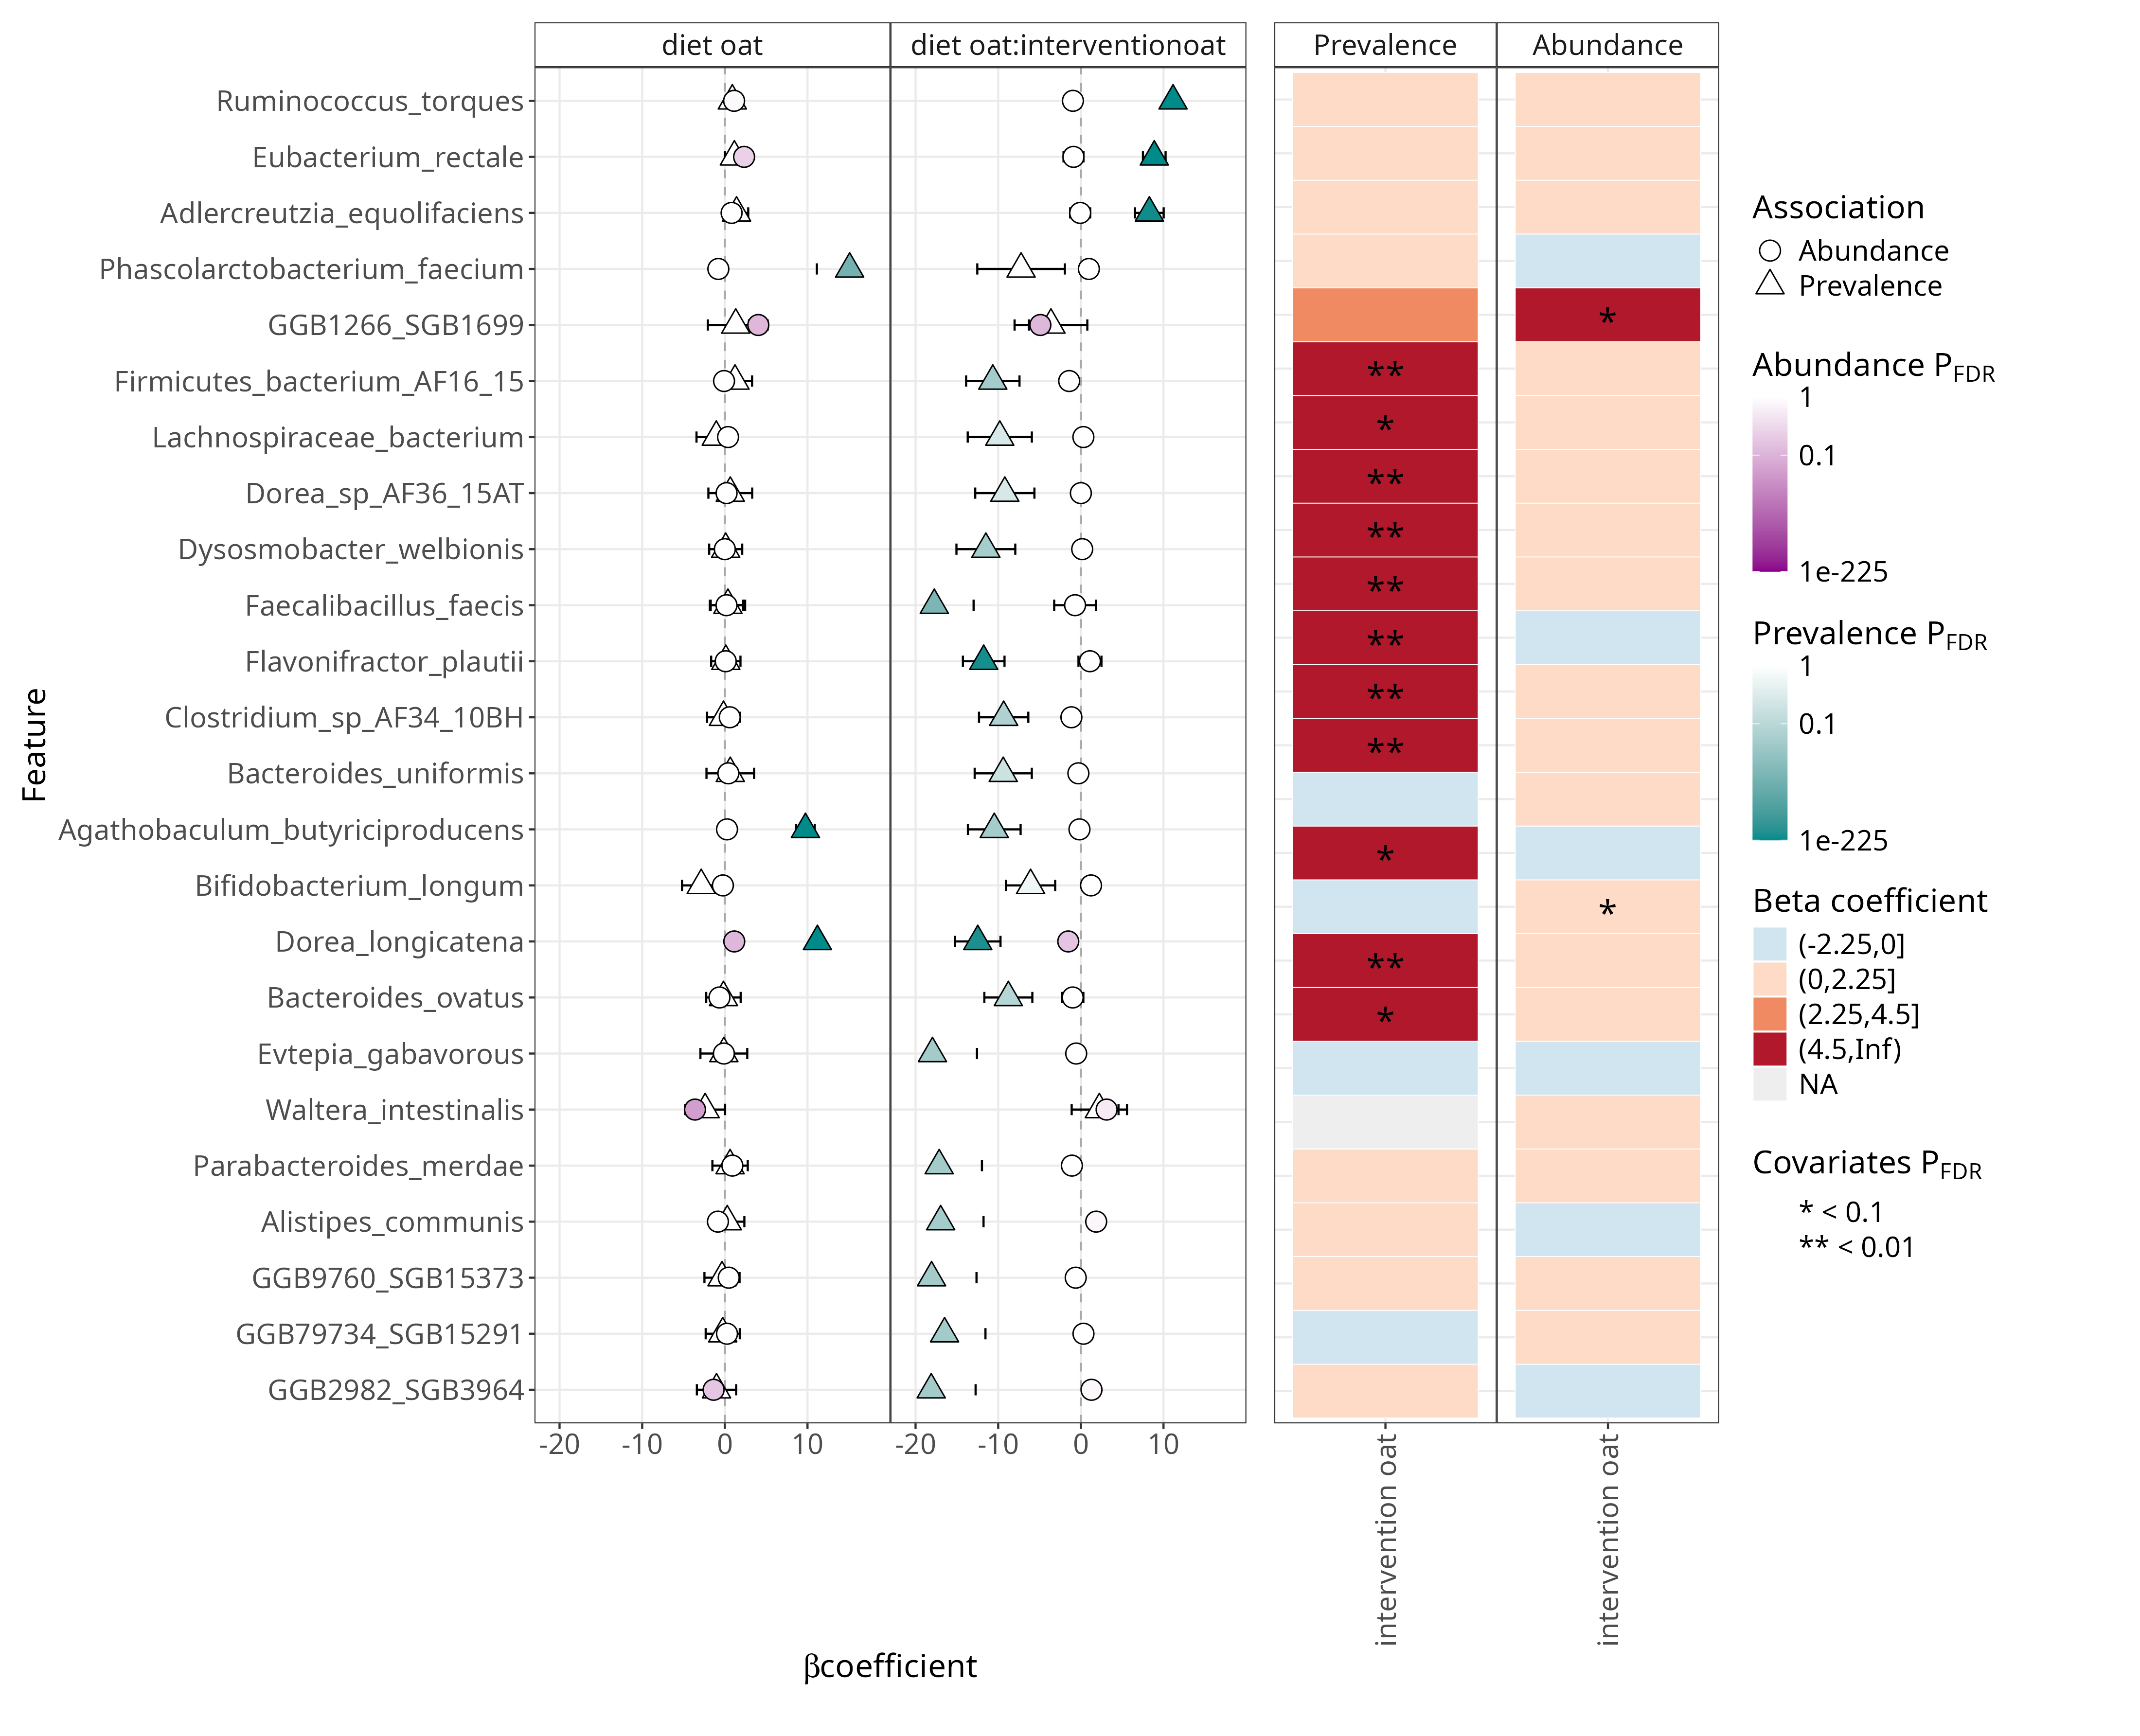
\includegraphics{../../output/daa/daa_taxa/species/figures/summary_plot.png}

}

\caption{taxa\_image18}

\end{figure}%

\subsubsection{family}\label{family}

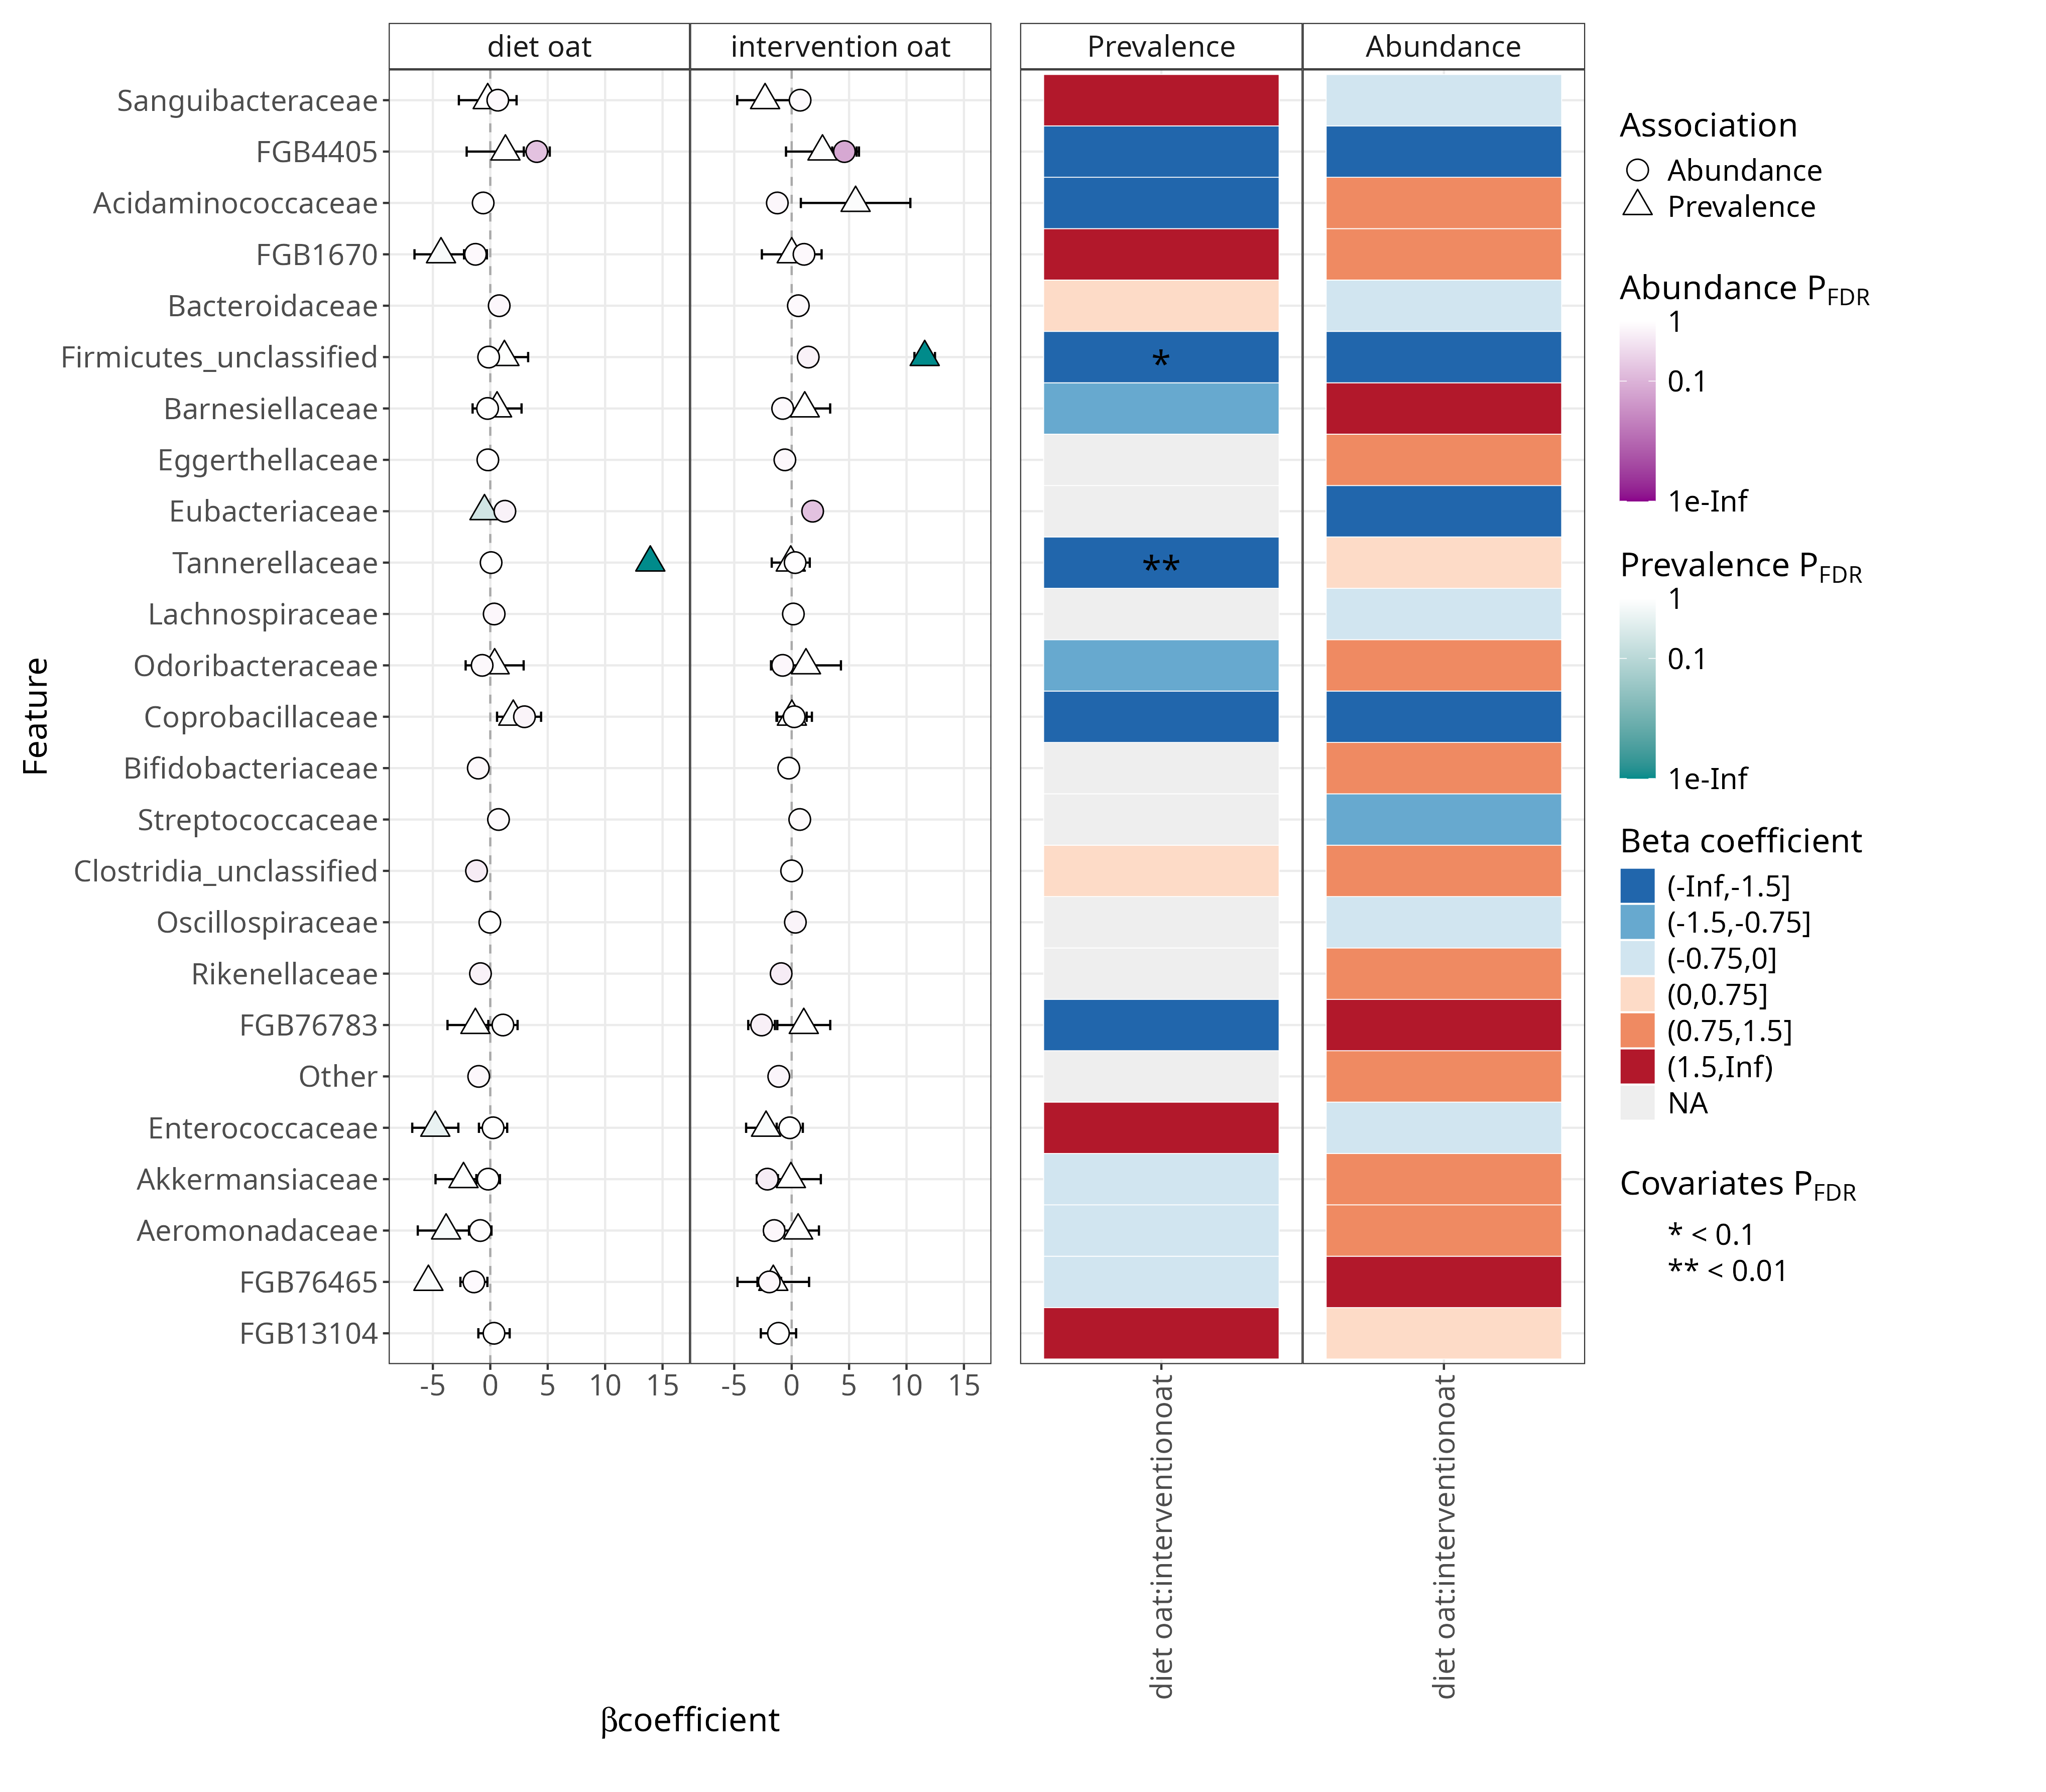
\includegraphics{../../output/daa/daa_taxa/family/figures/summary_plot.png}\\

\subsubsection{genus}\label{genus}

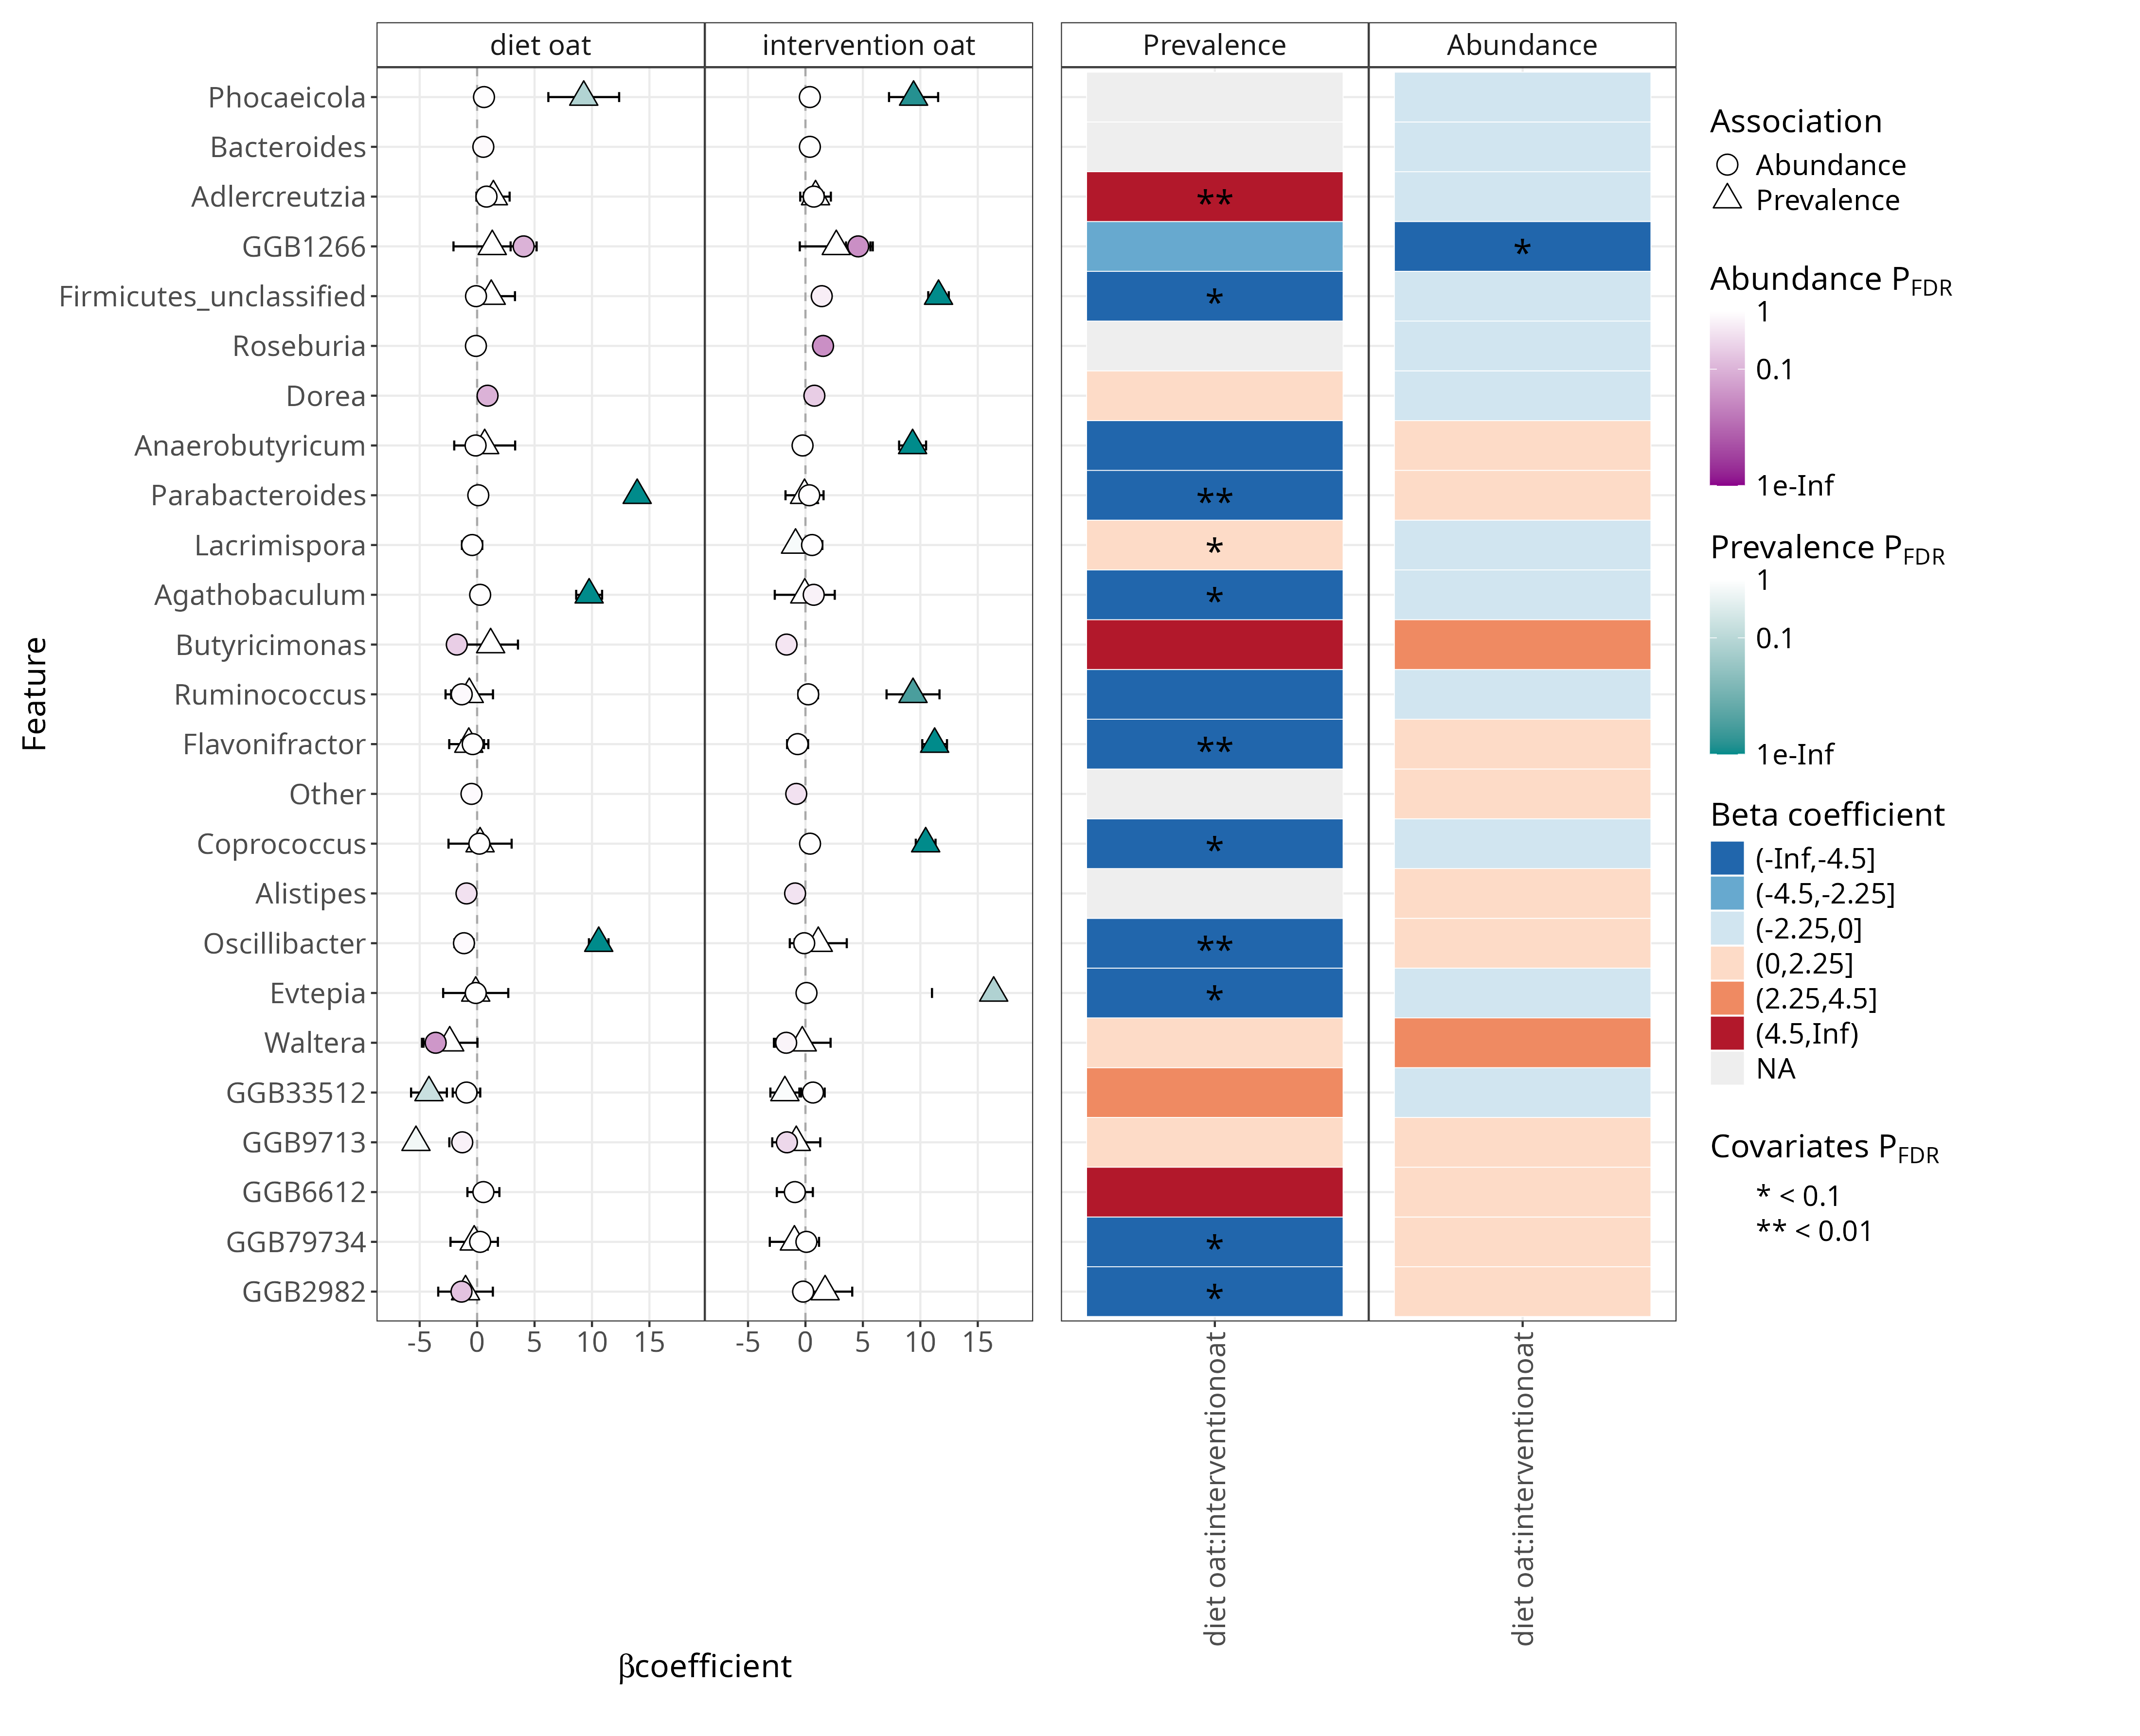
\includegraphics{../../output/daa/daa_taxa/genus/figures/summary_plot.png}\\

\subsubsection{phylum}\label{phylum}

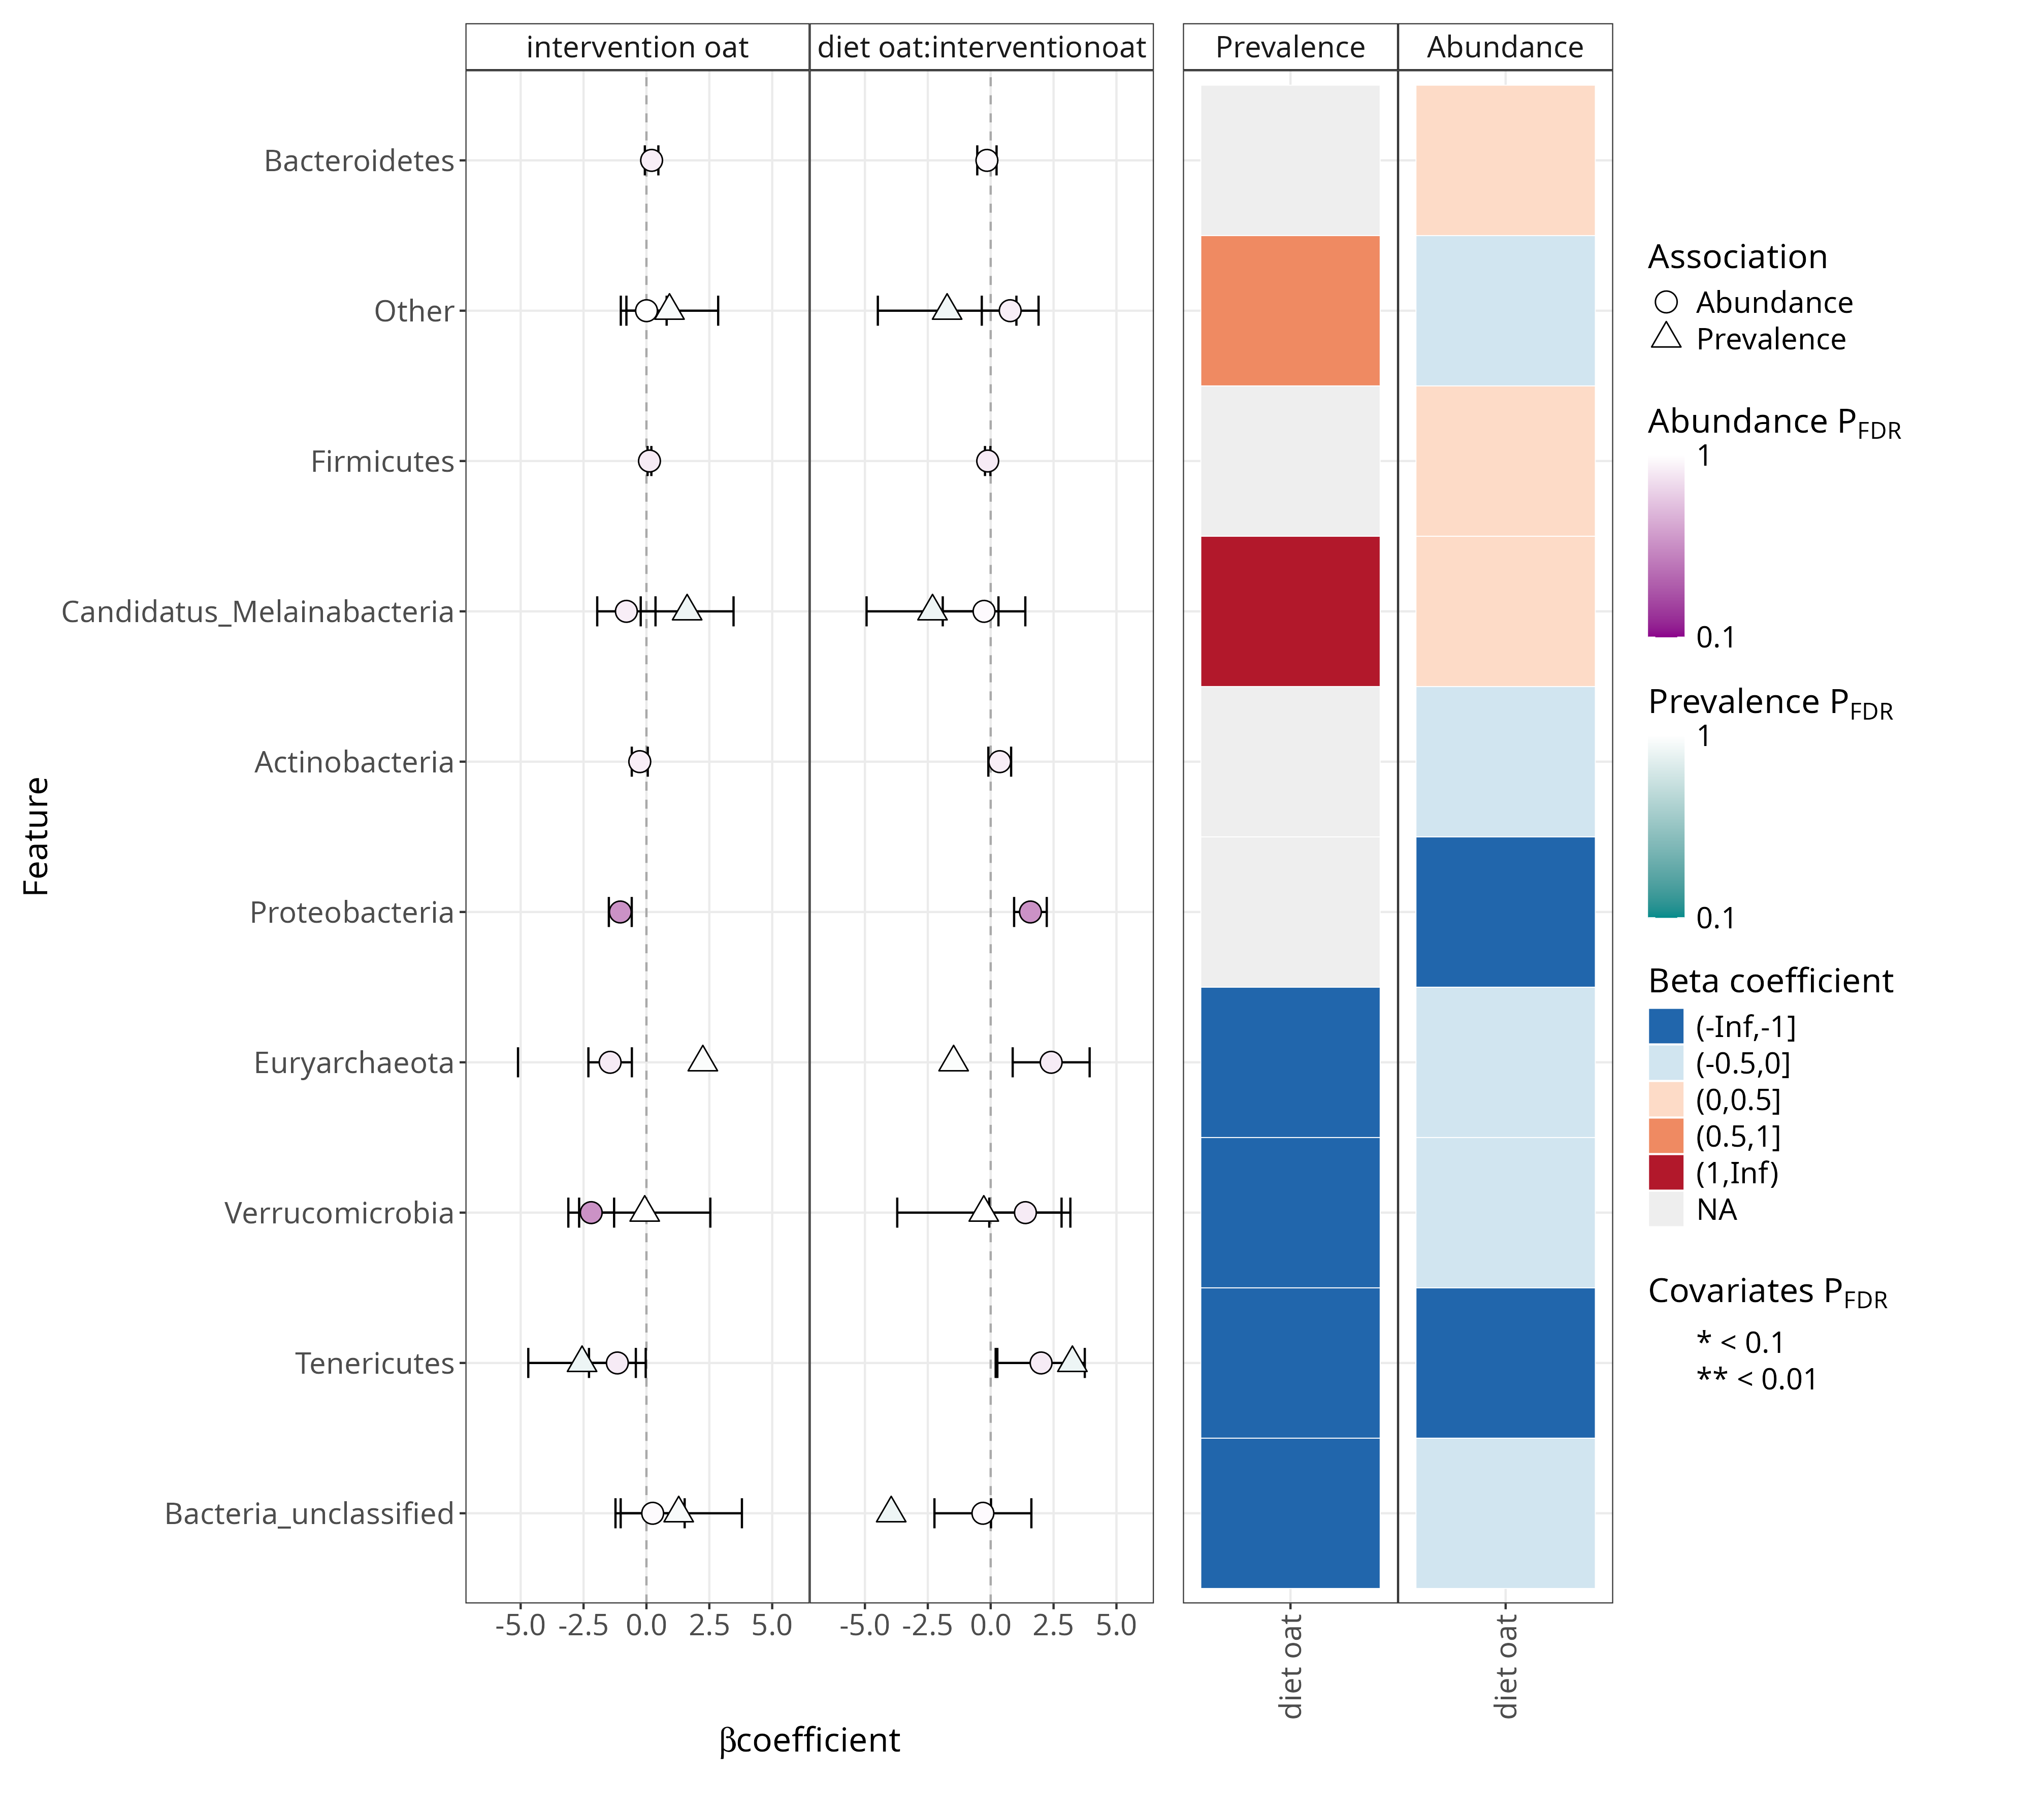
\includegraphics{../../output/daa/daa_taxa/phylum/figures/summary_plot.png}\\

\subsection{Associations plots}\label{associations-plots}

Box plots are used for categorical data abundance associations. Grids
are used for categorical data prevalence associations. Data points
plotted are after filtering, normalization, and transformation so that
the scale in the plot is the scale that was used in fitting.

\subsubsection{Associations-species}\label{associations-species}

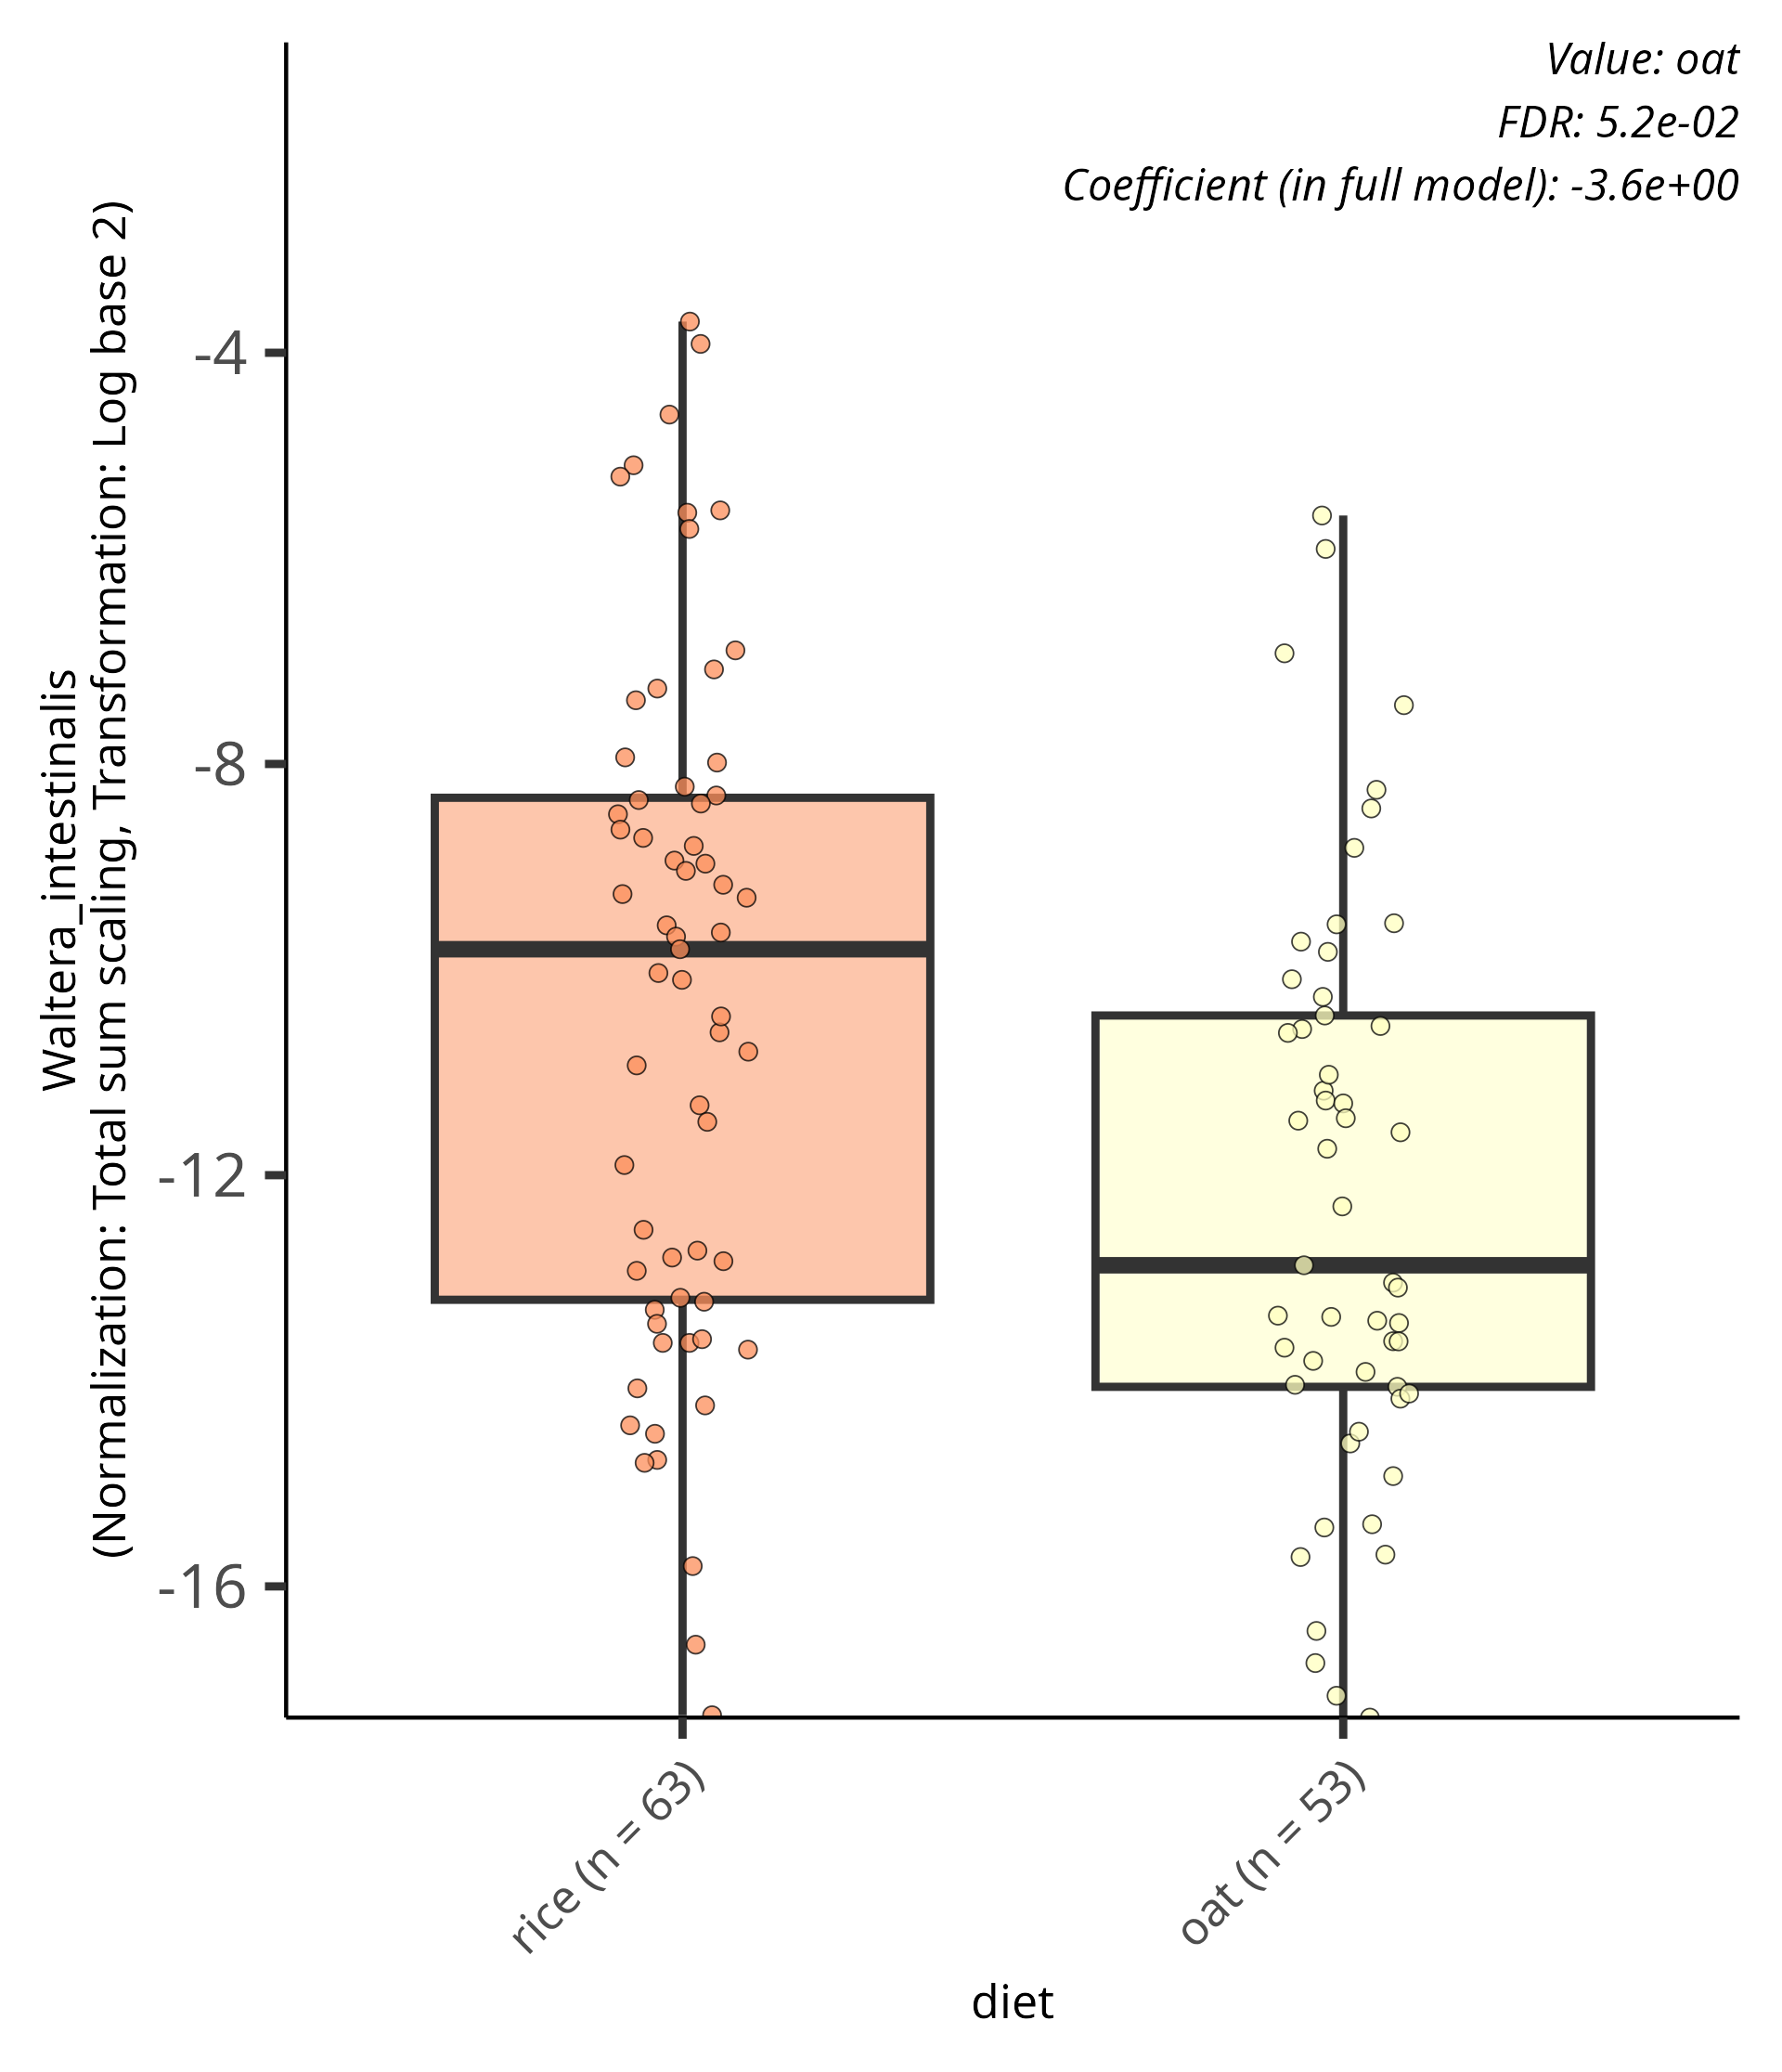
\includegraphics{../../output/daa/daa_taxa/species/figures/association_plots/diet/linear/diet_Waltera_intestinalis_linear.png}\\
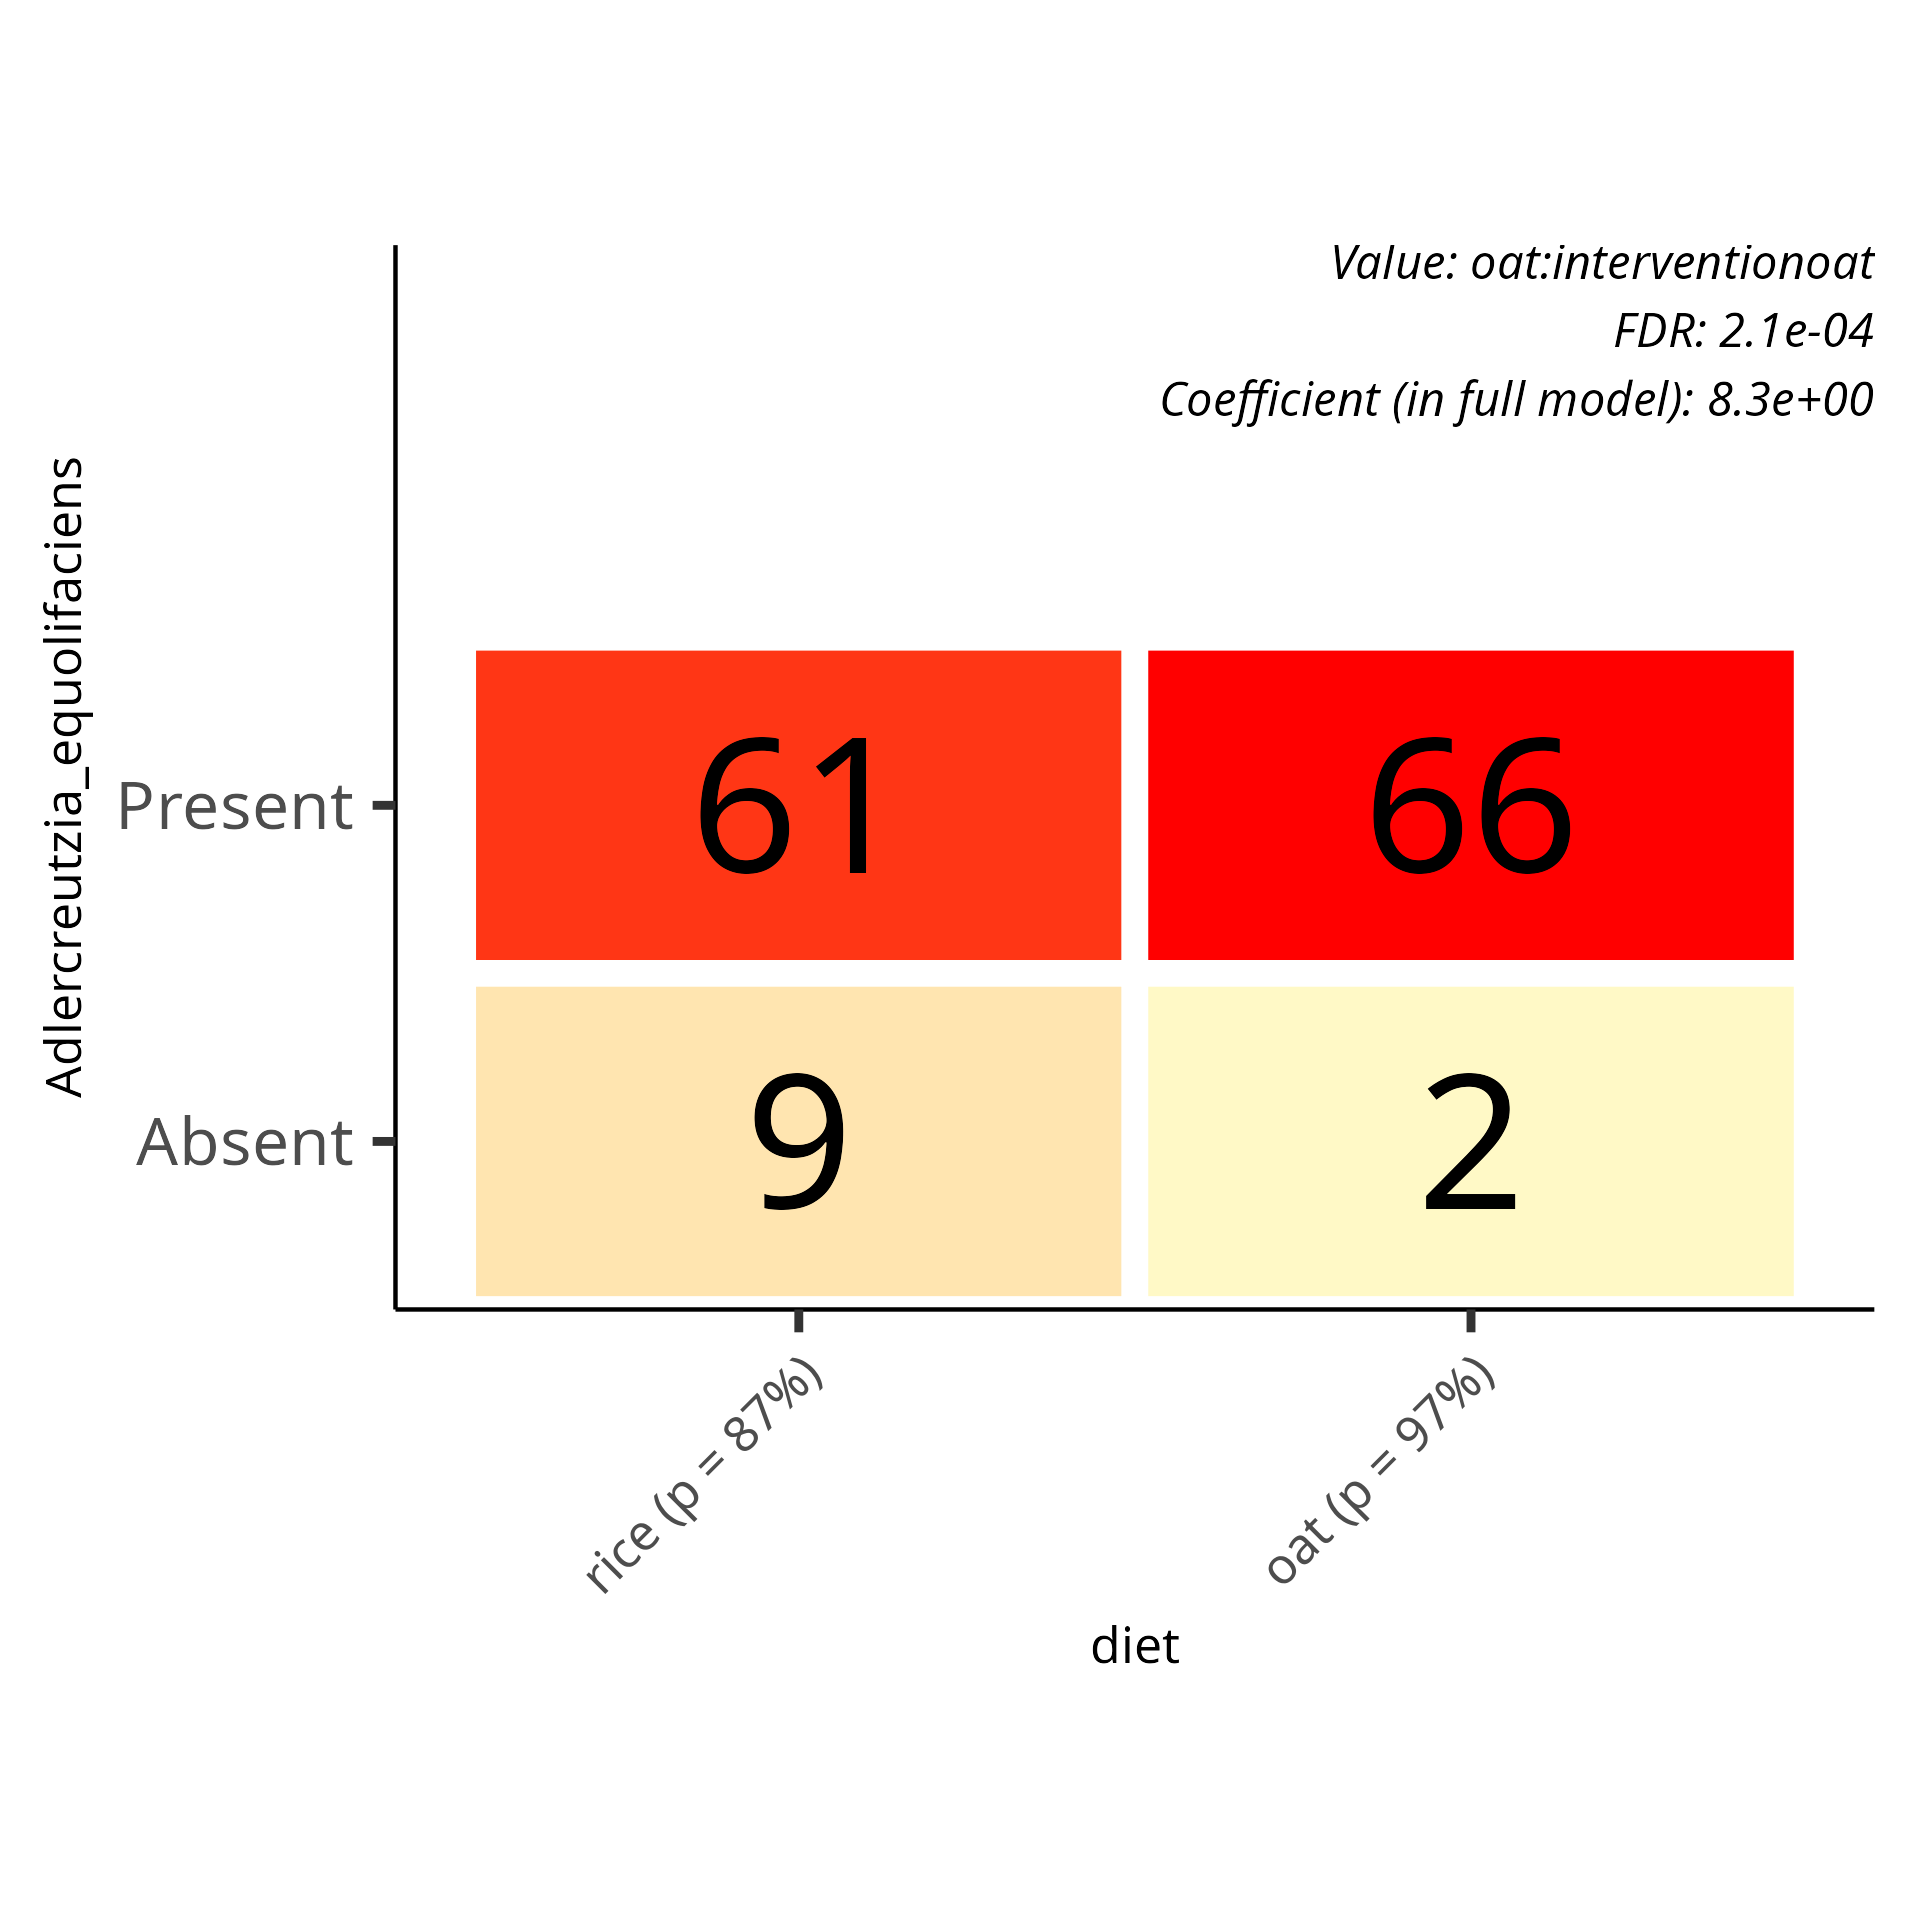
\includegraphics{../../output/daa/daa_taxa/species/figures/association_plots/diet/logistic/diet_Adlercreutzia_equolifaciens_logistic.png}\\
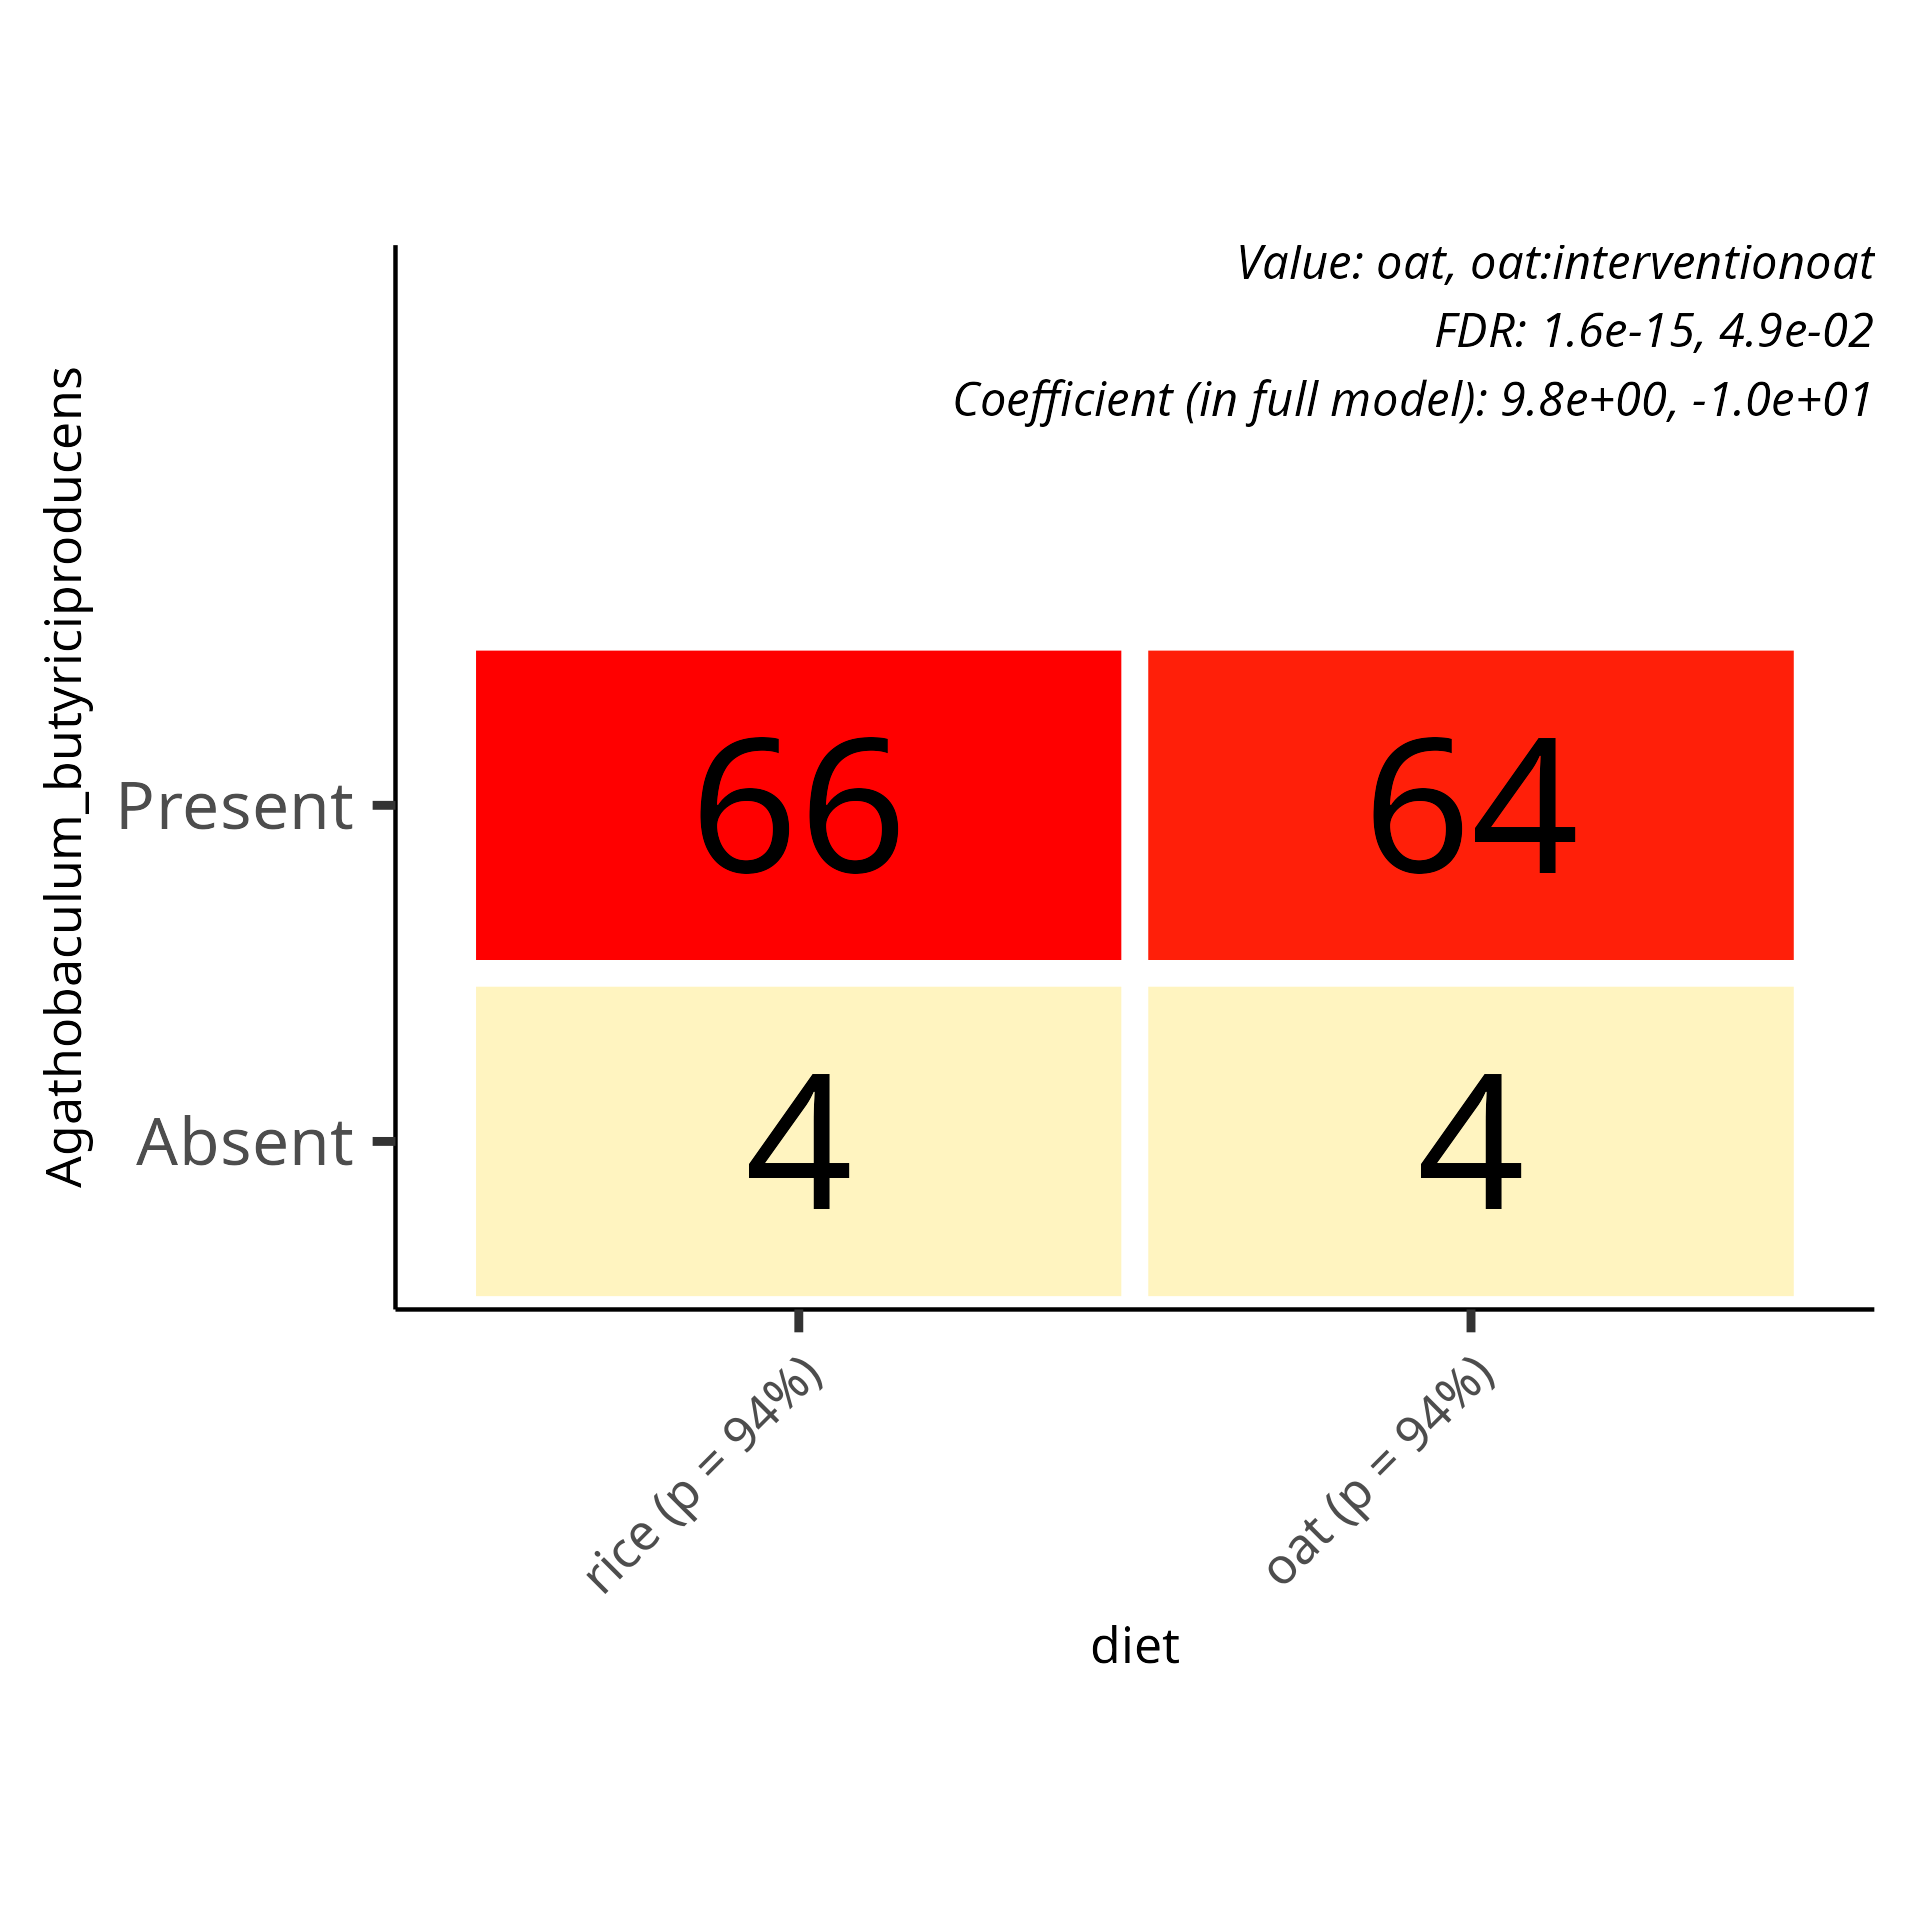
\includegraphics{../../output/daa/daa_taxa/species/figures/association_plots/diet/logistic/diet_Agathobaculum_butyriciproducens_logistic.png}\\
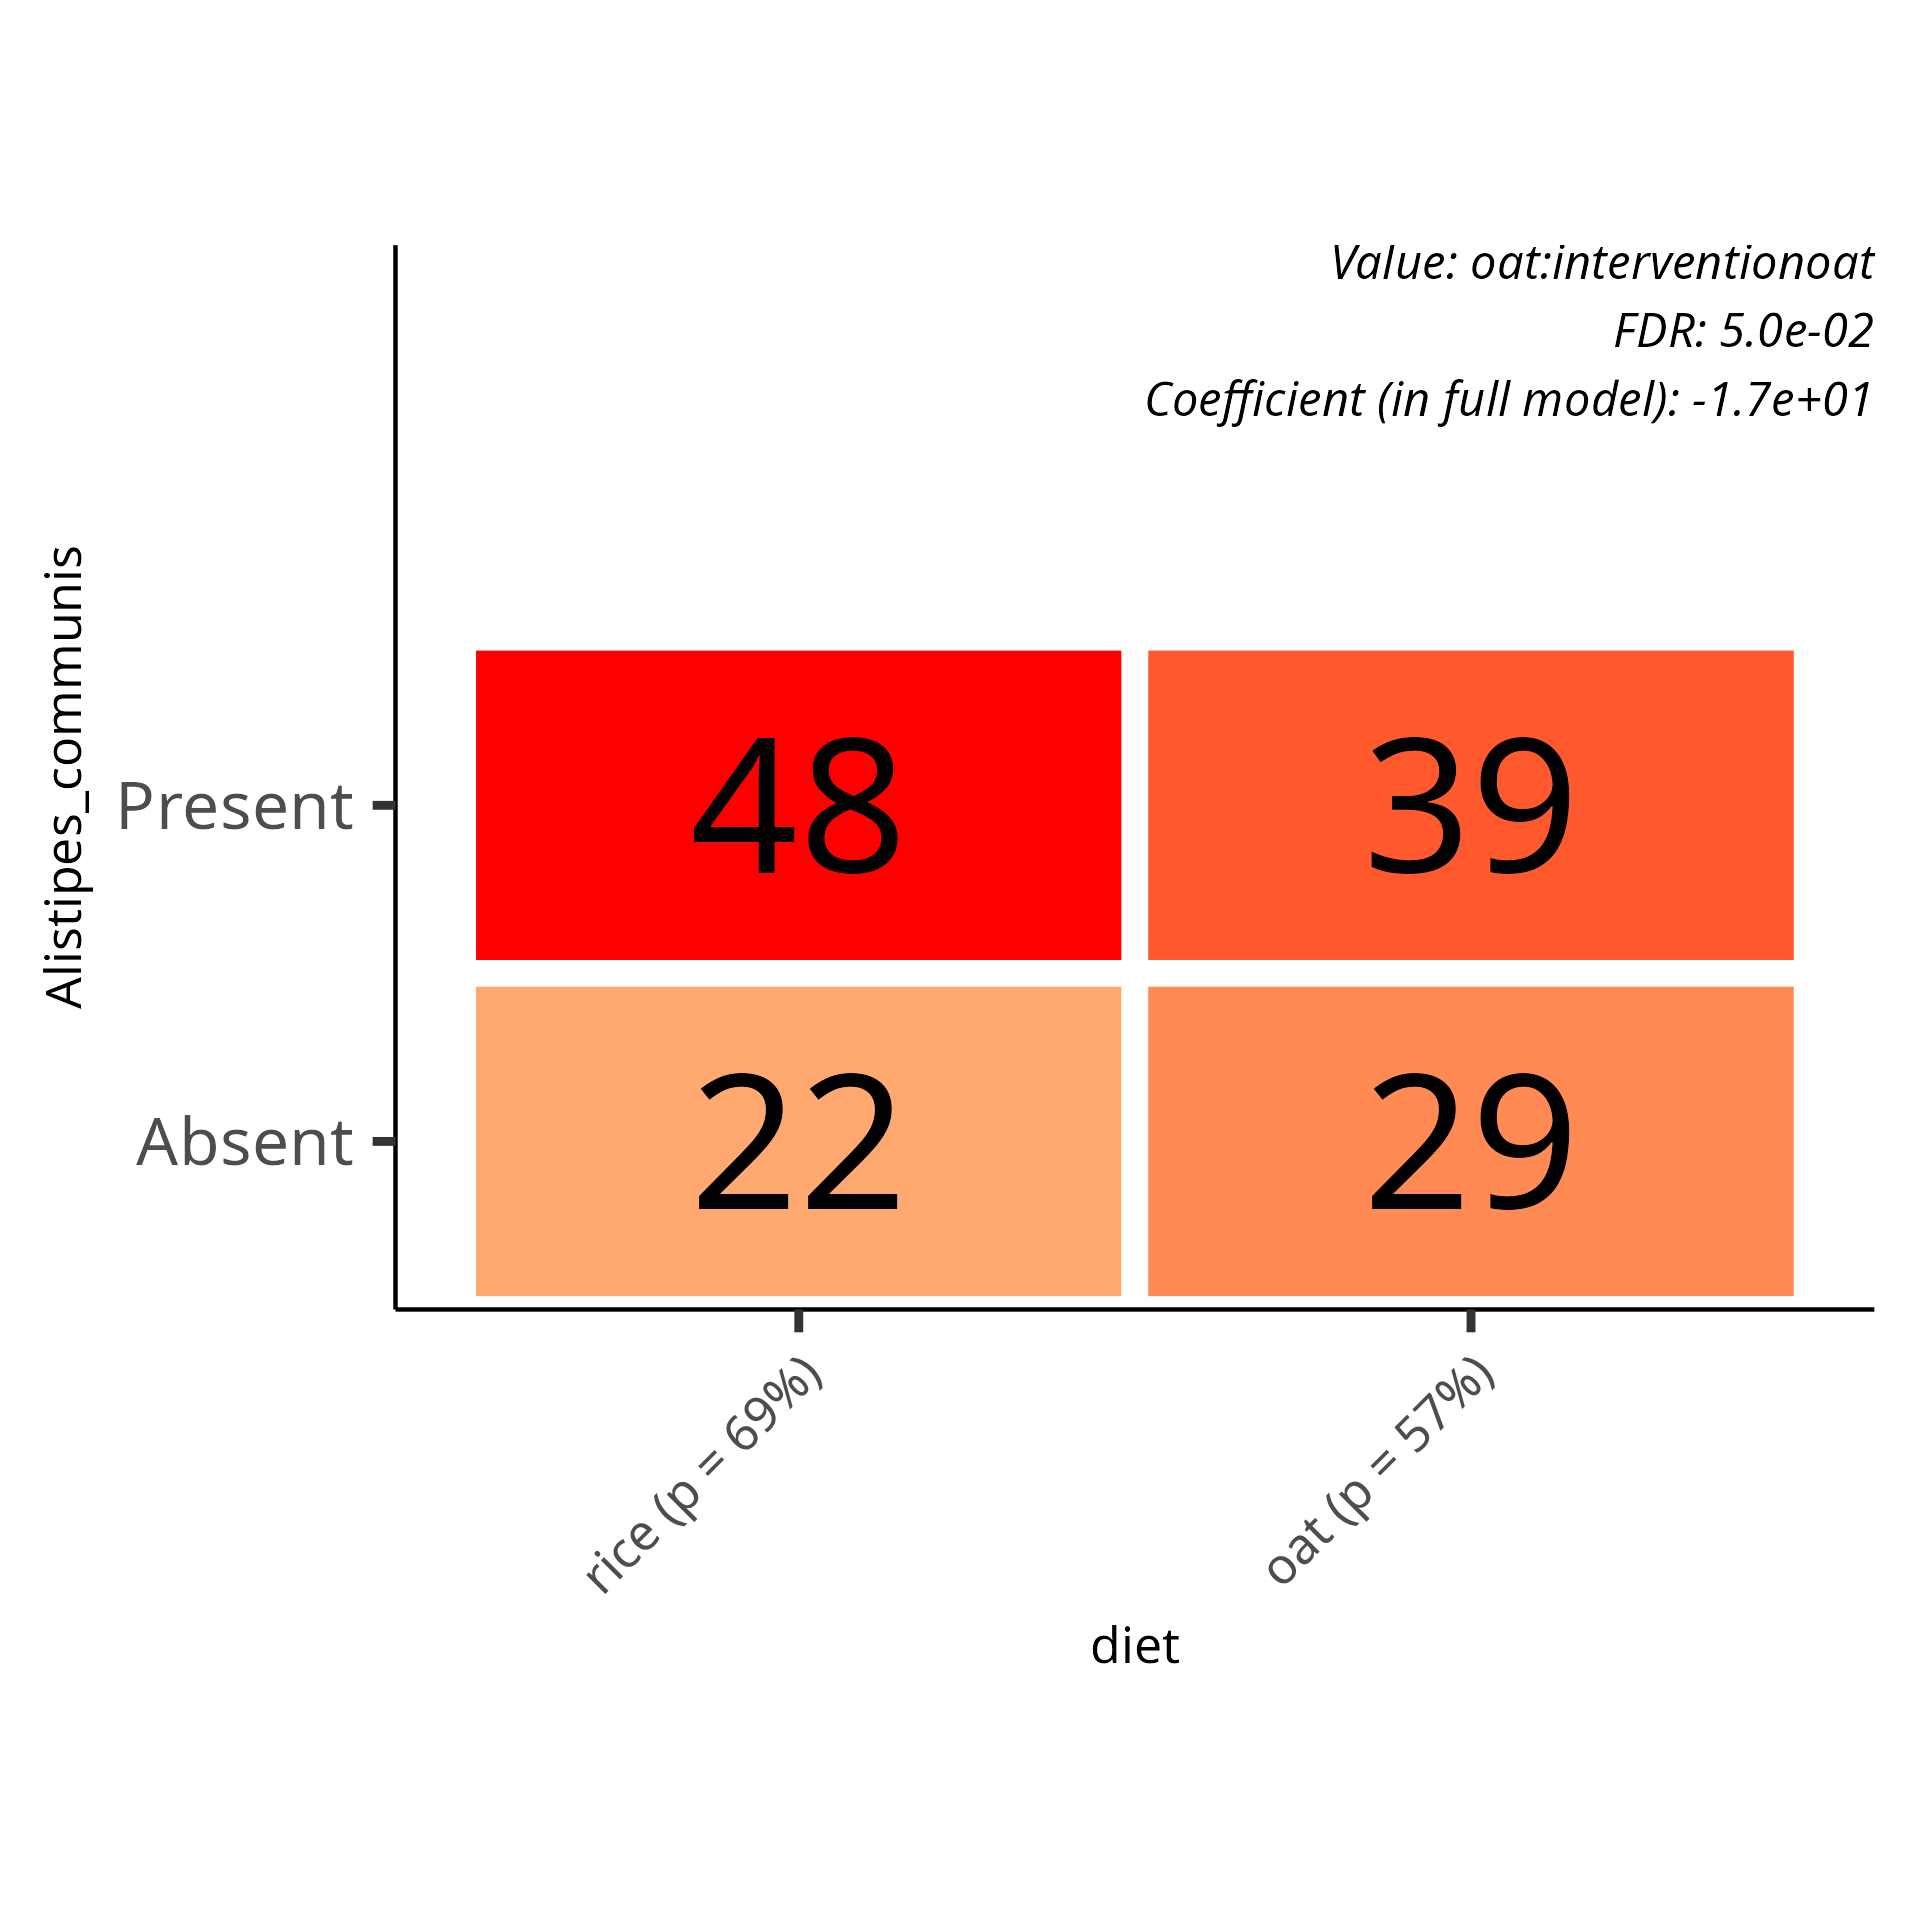
\includegraphics{../../output/daa/daa_taxa/species/figures/association_plots/diet/logistic/diet_Alistipes_communis_logistic.png}\\
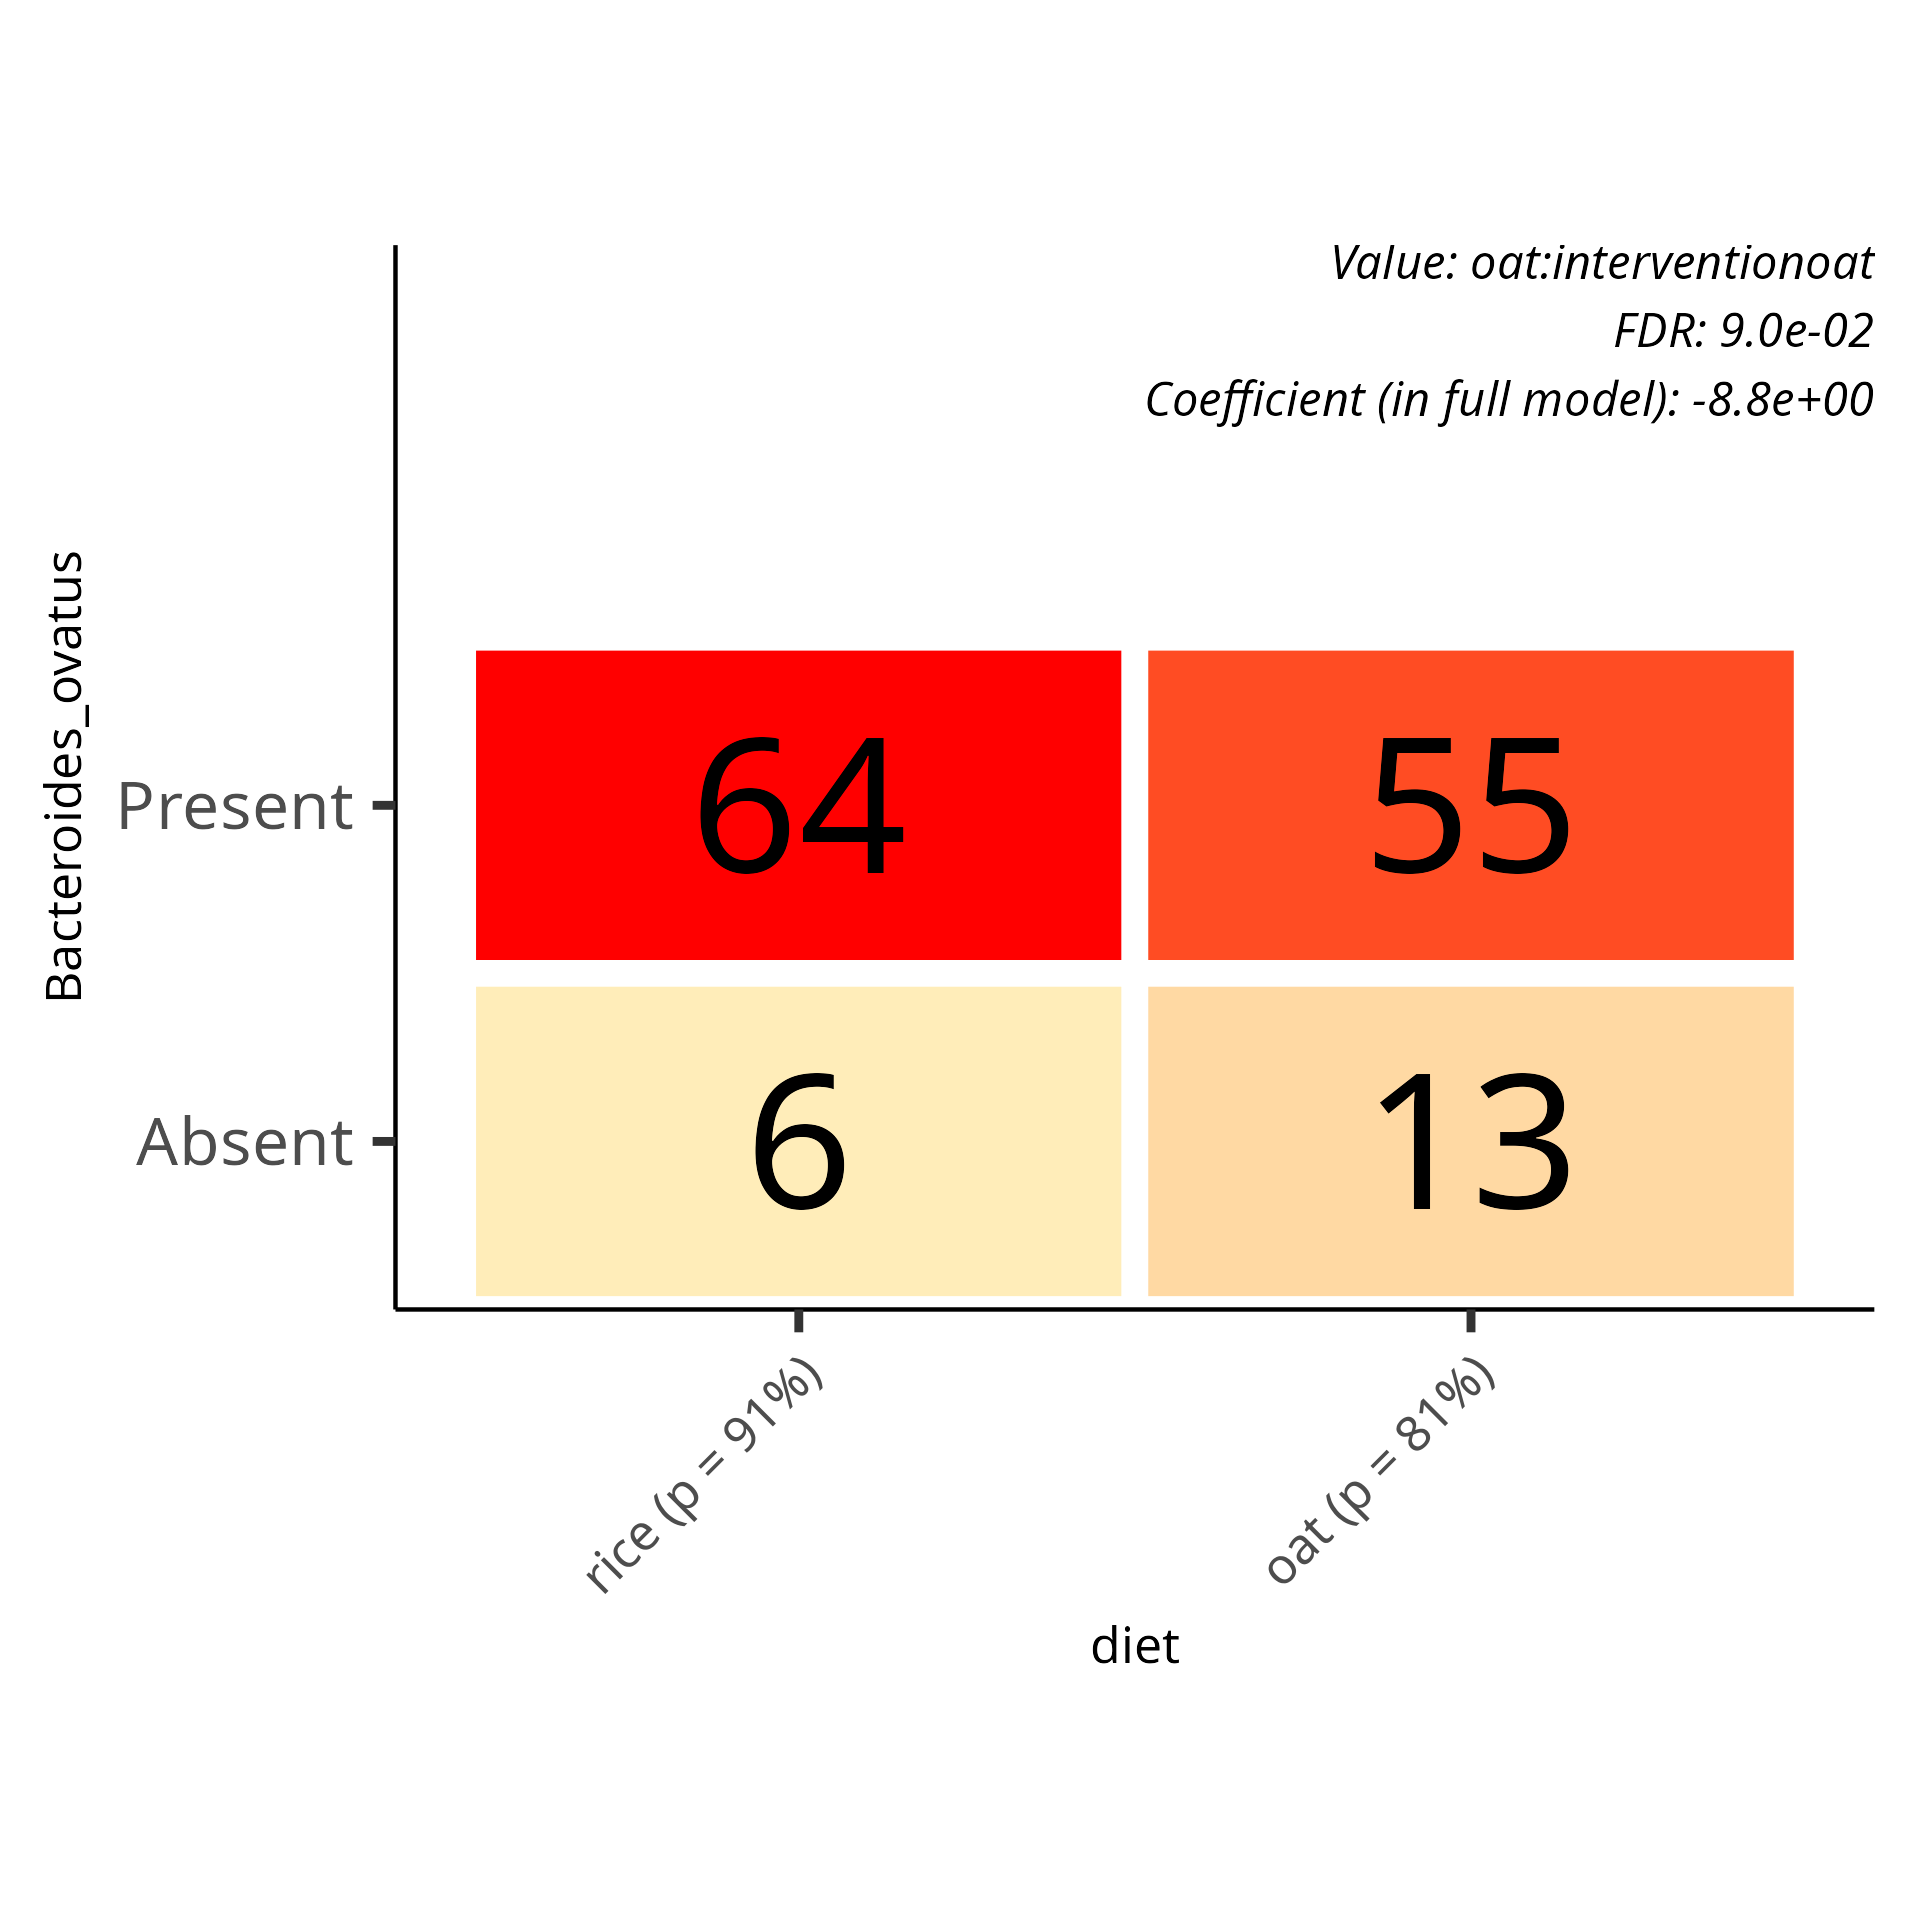
\includegraphics{../../output/daa/daa_taxa/species/figures/association_plots/diet/logistic/diet_Bacteroides_ovatus_logistic.png}\\
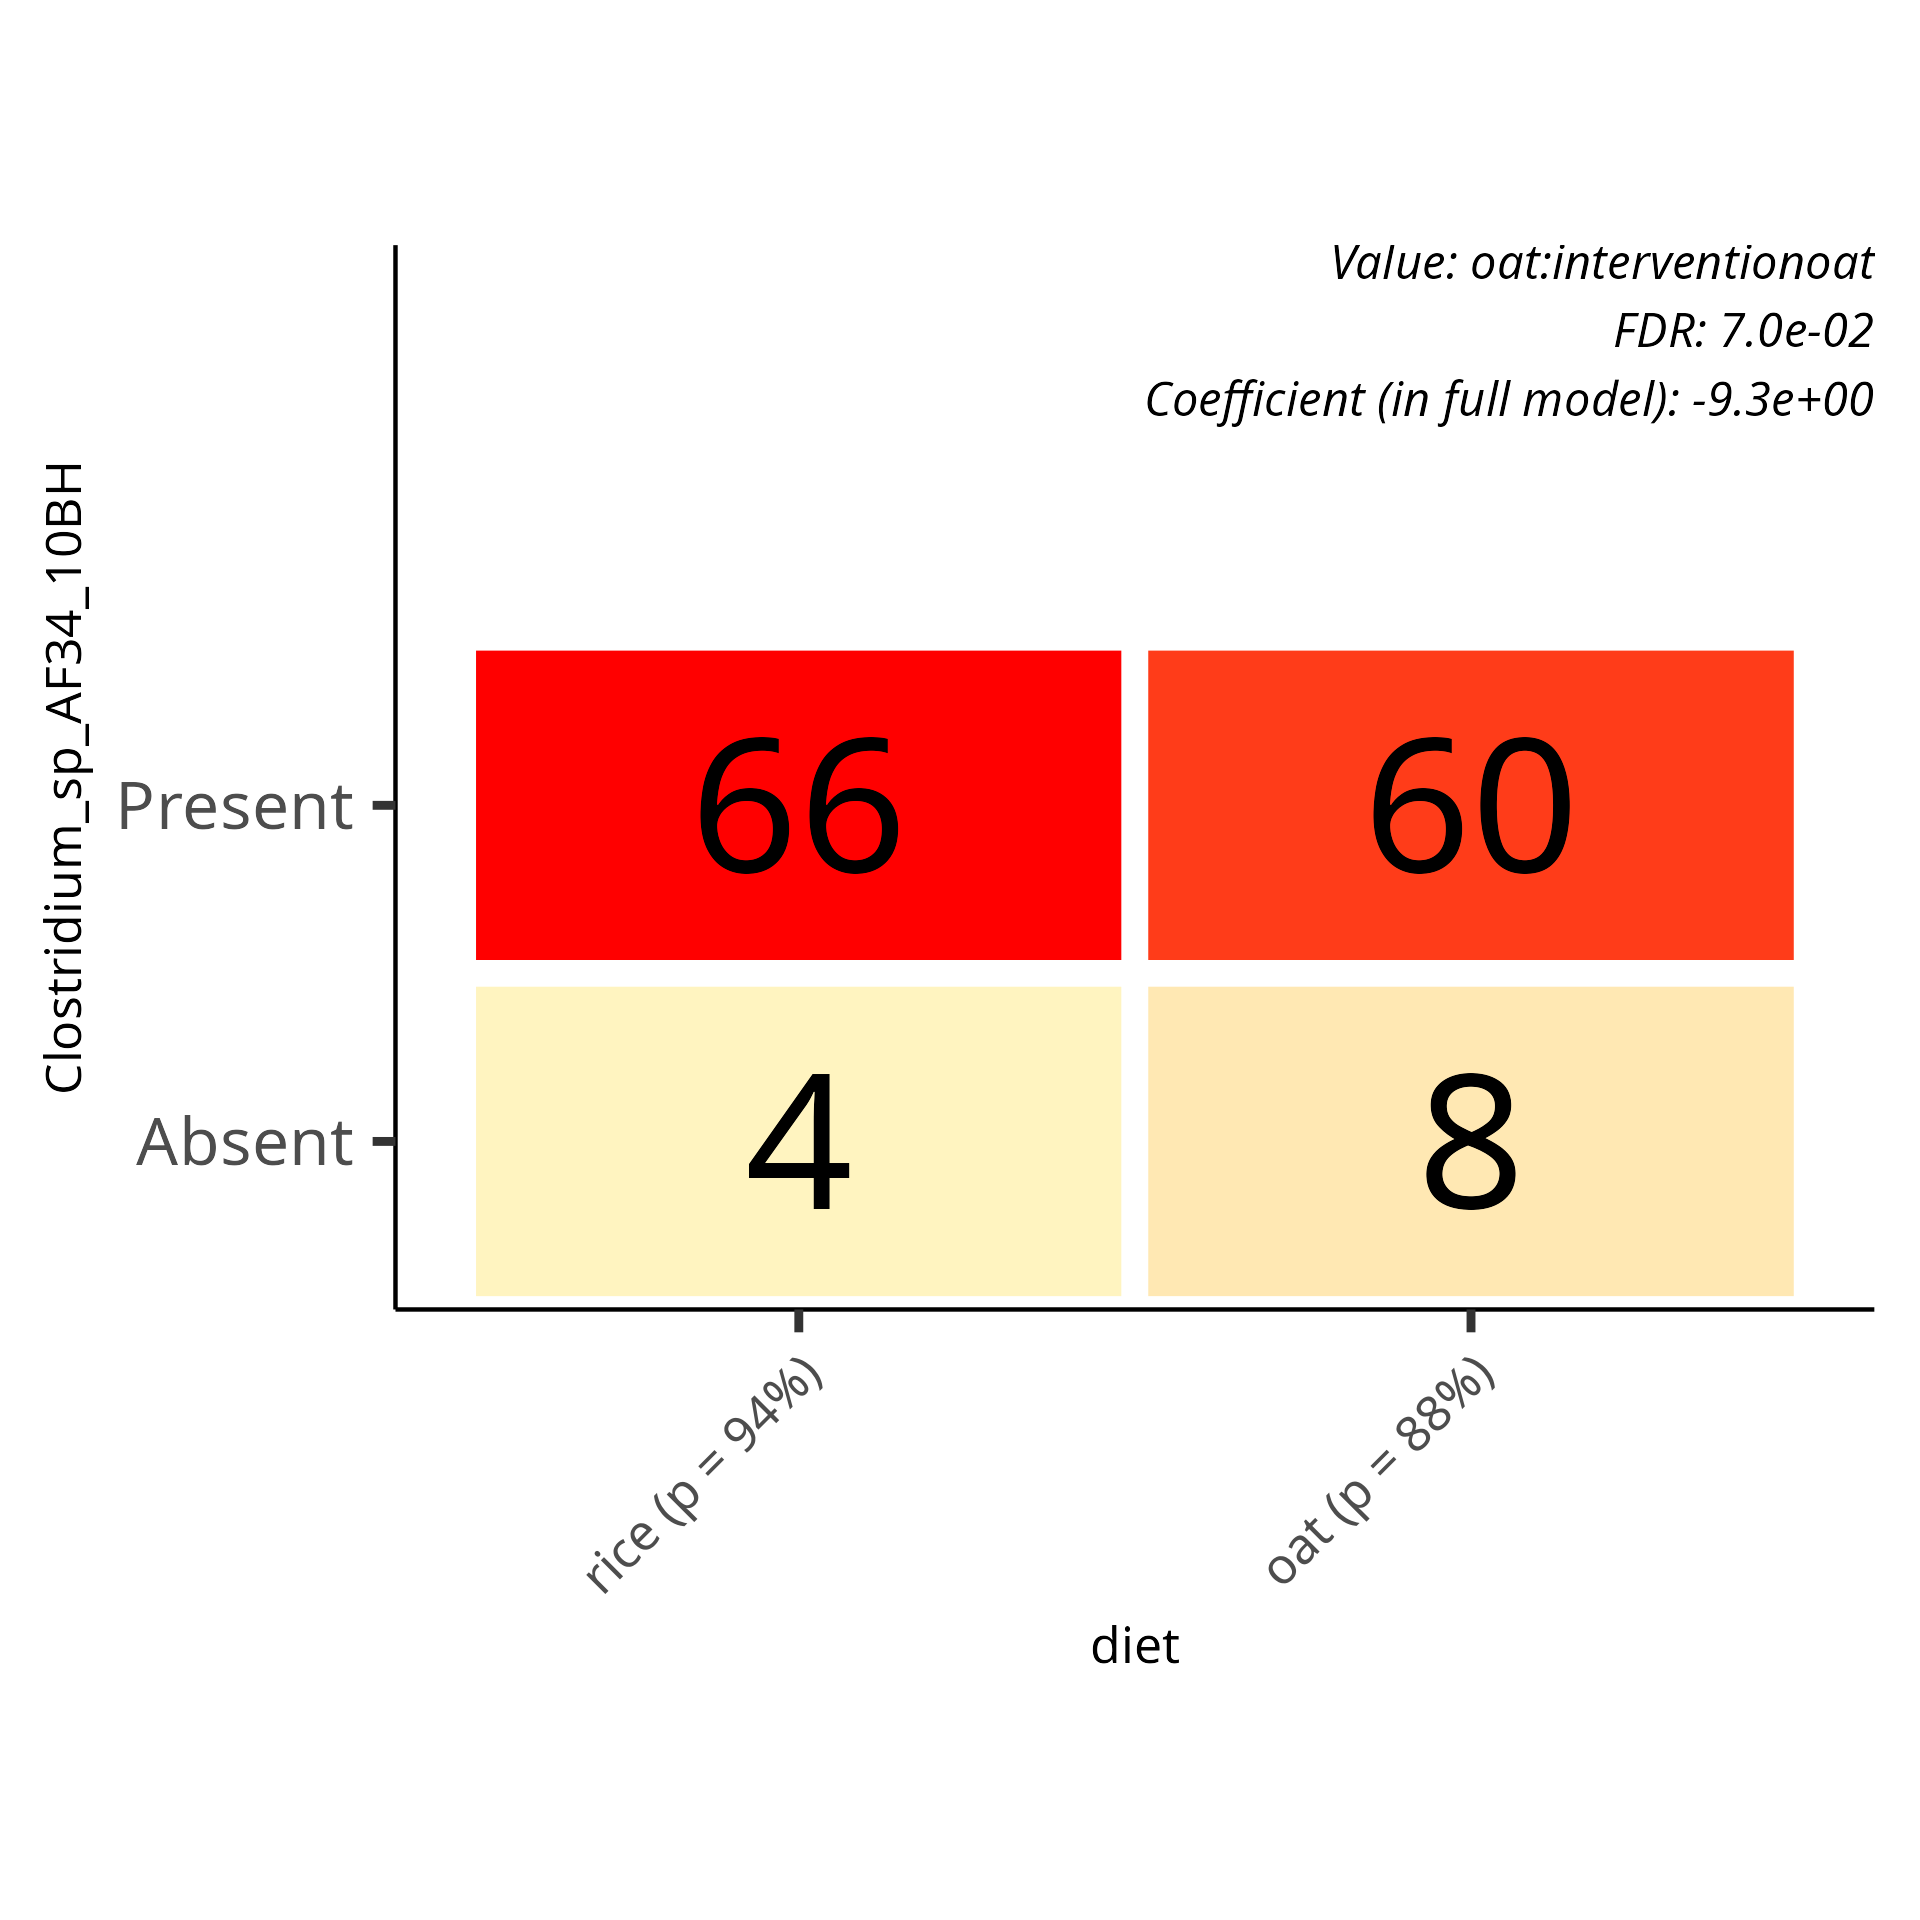
\includegraphics{../../output/daa/daa_taxa/species/figures/association_plots/diet/logistic/diet_Clostridium_sp_AF34_10BH_logistic.png}\\
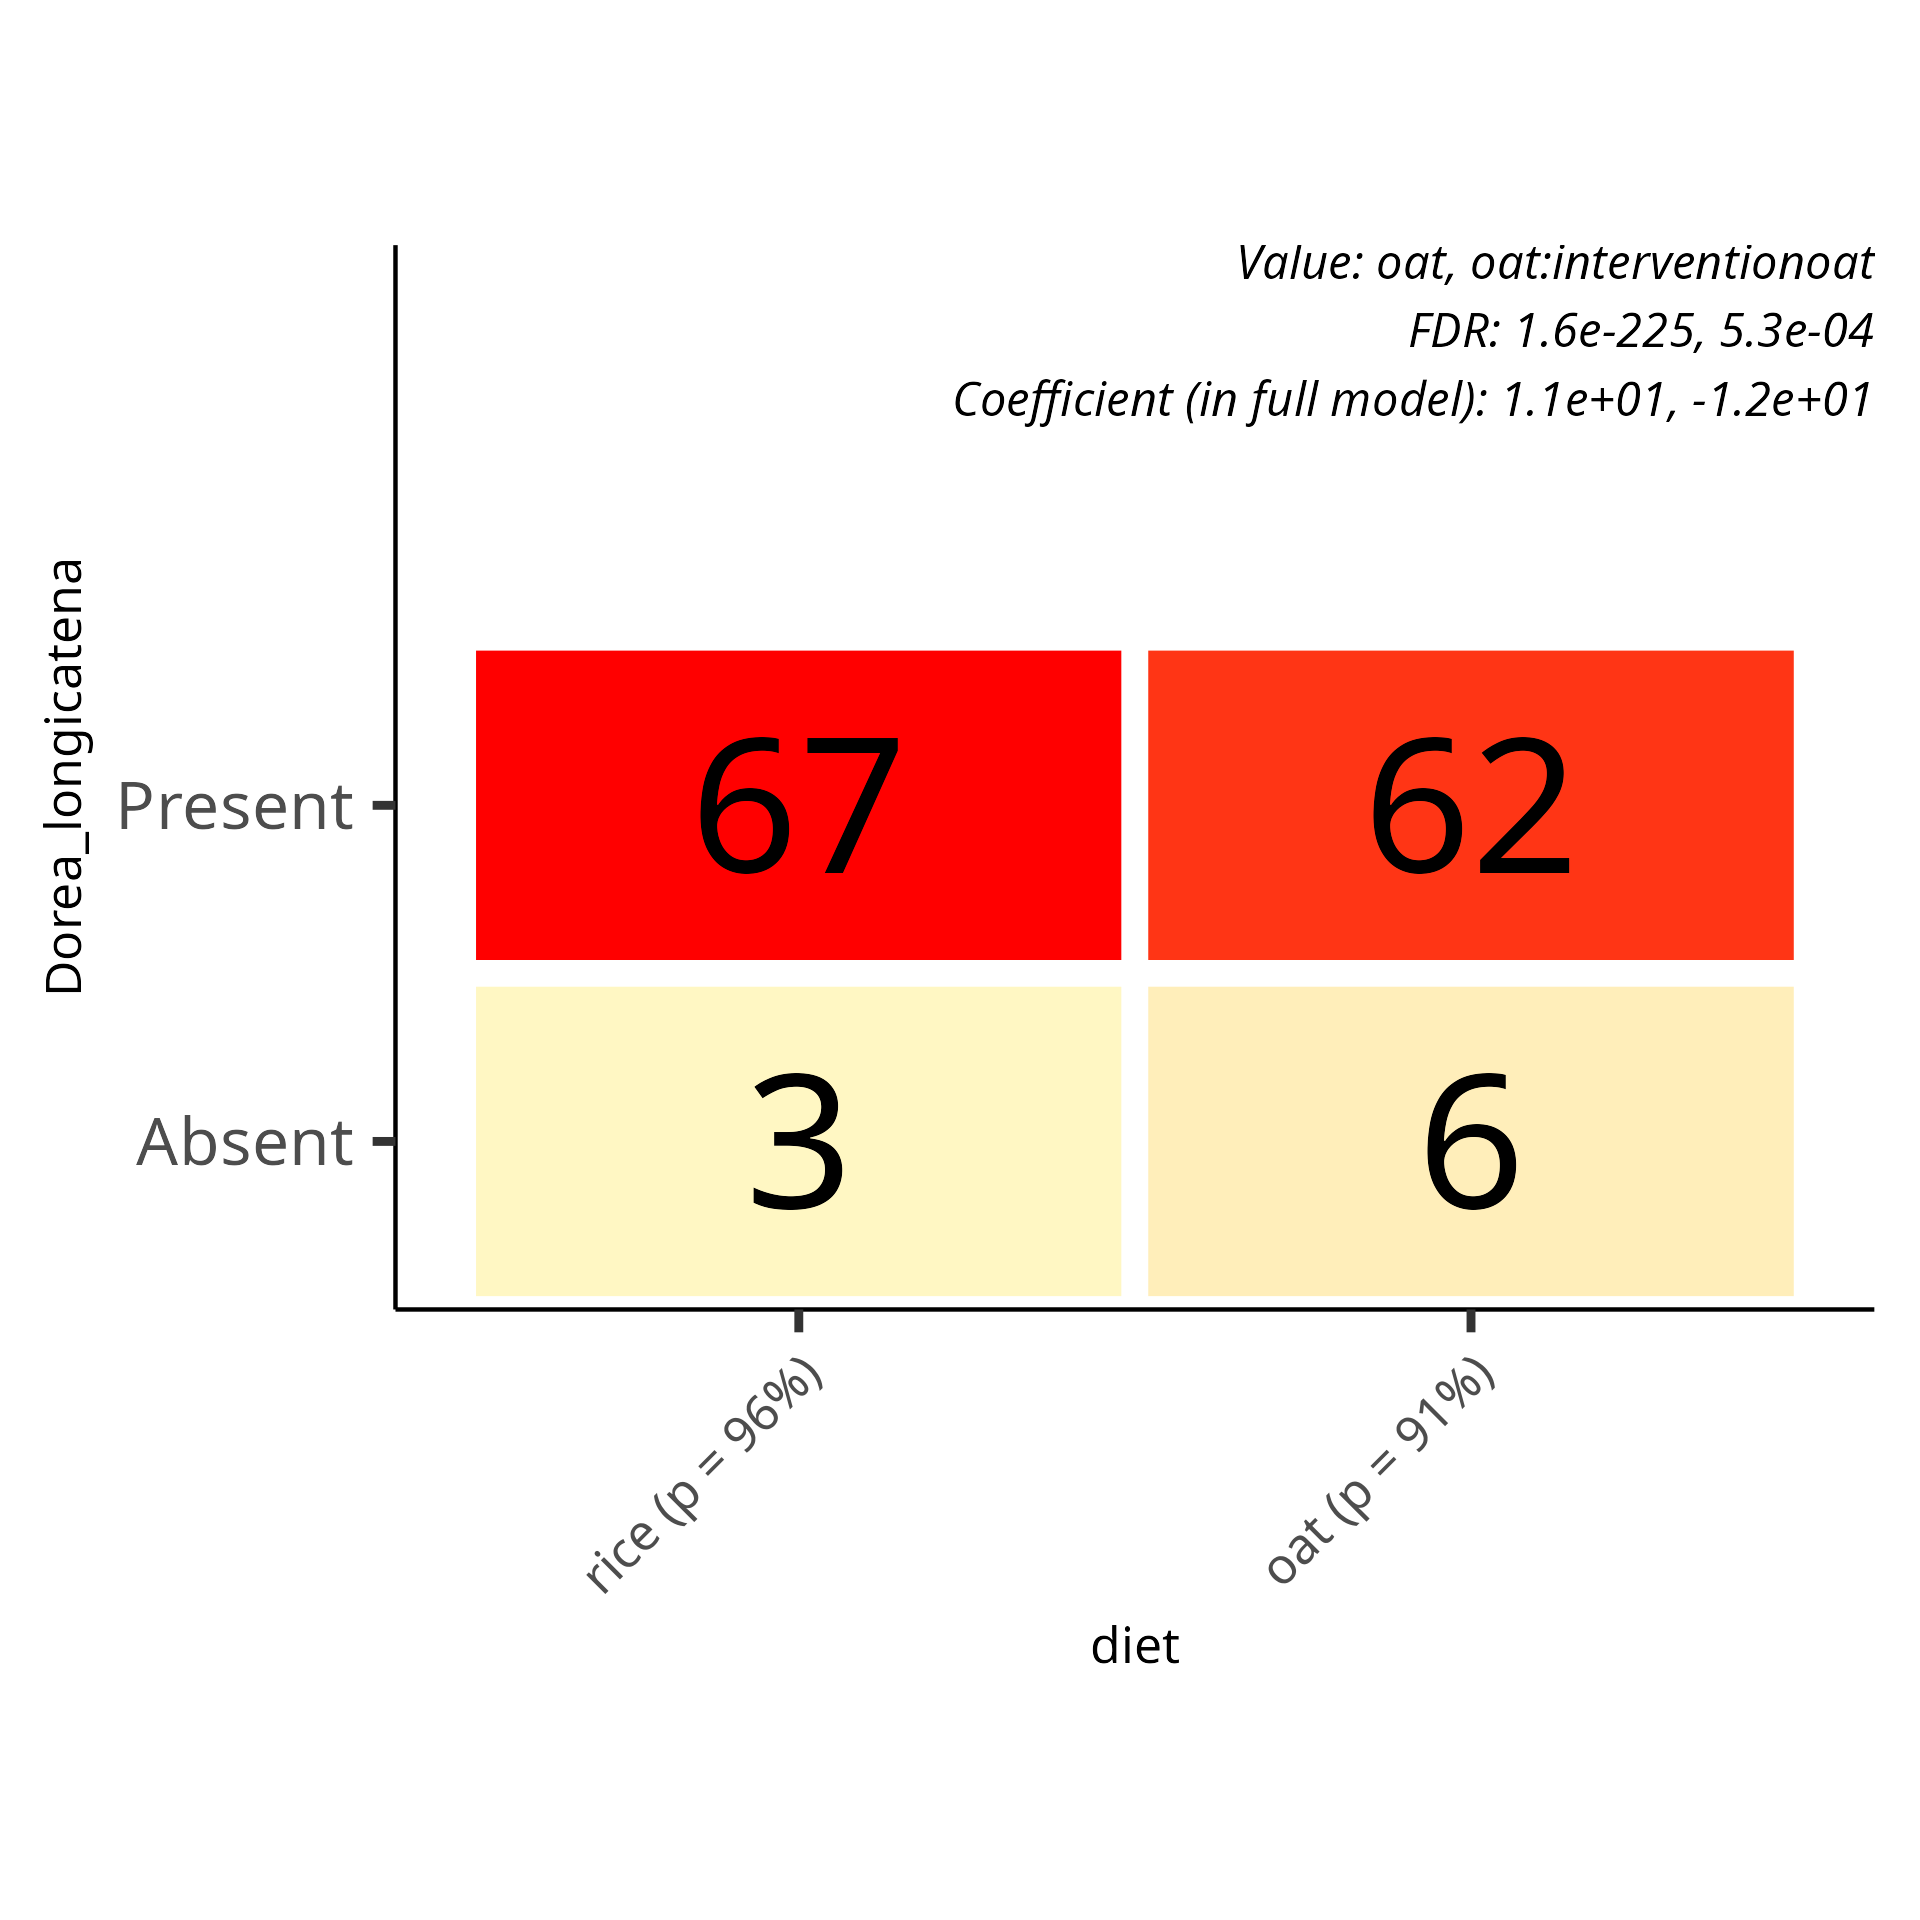
\includegraphics{../../output/daa/daa_taxa/species/figures/association_plots/diet/logistic/diet_Dorea_longicatena_logistic.png}\\
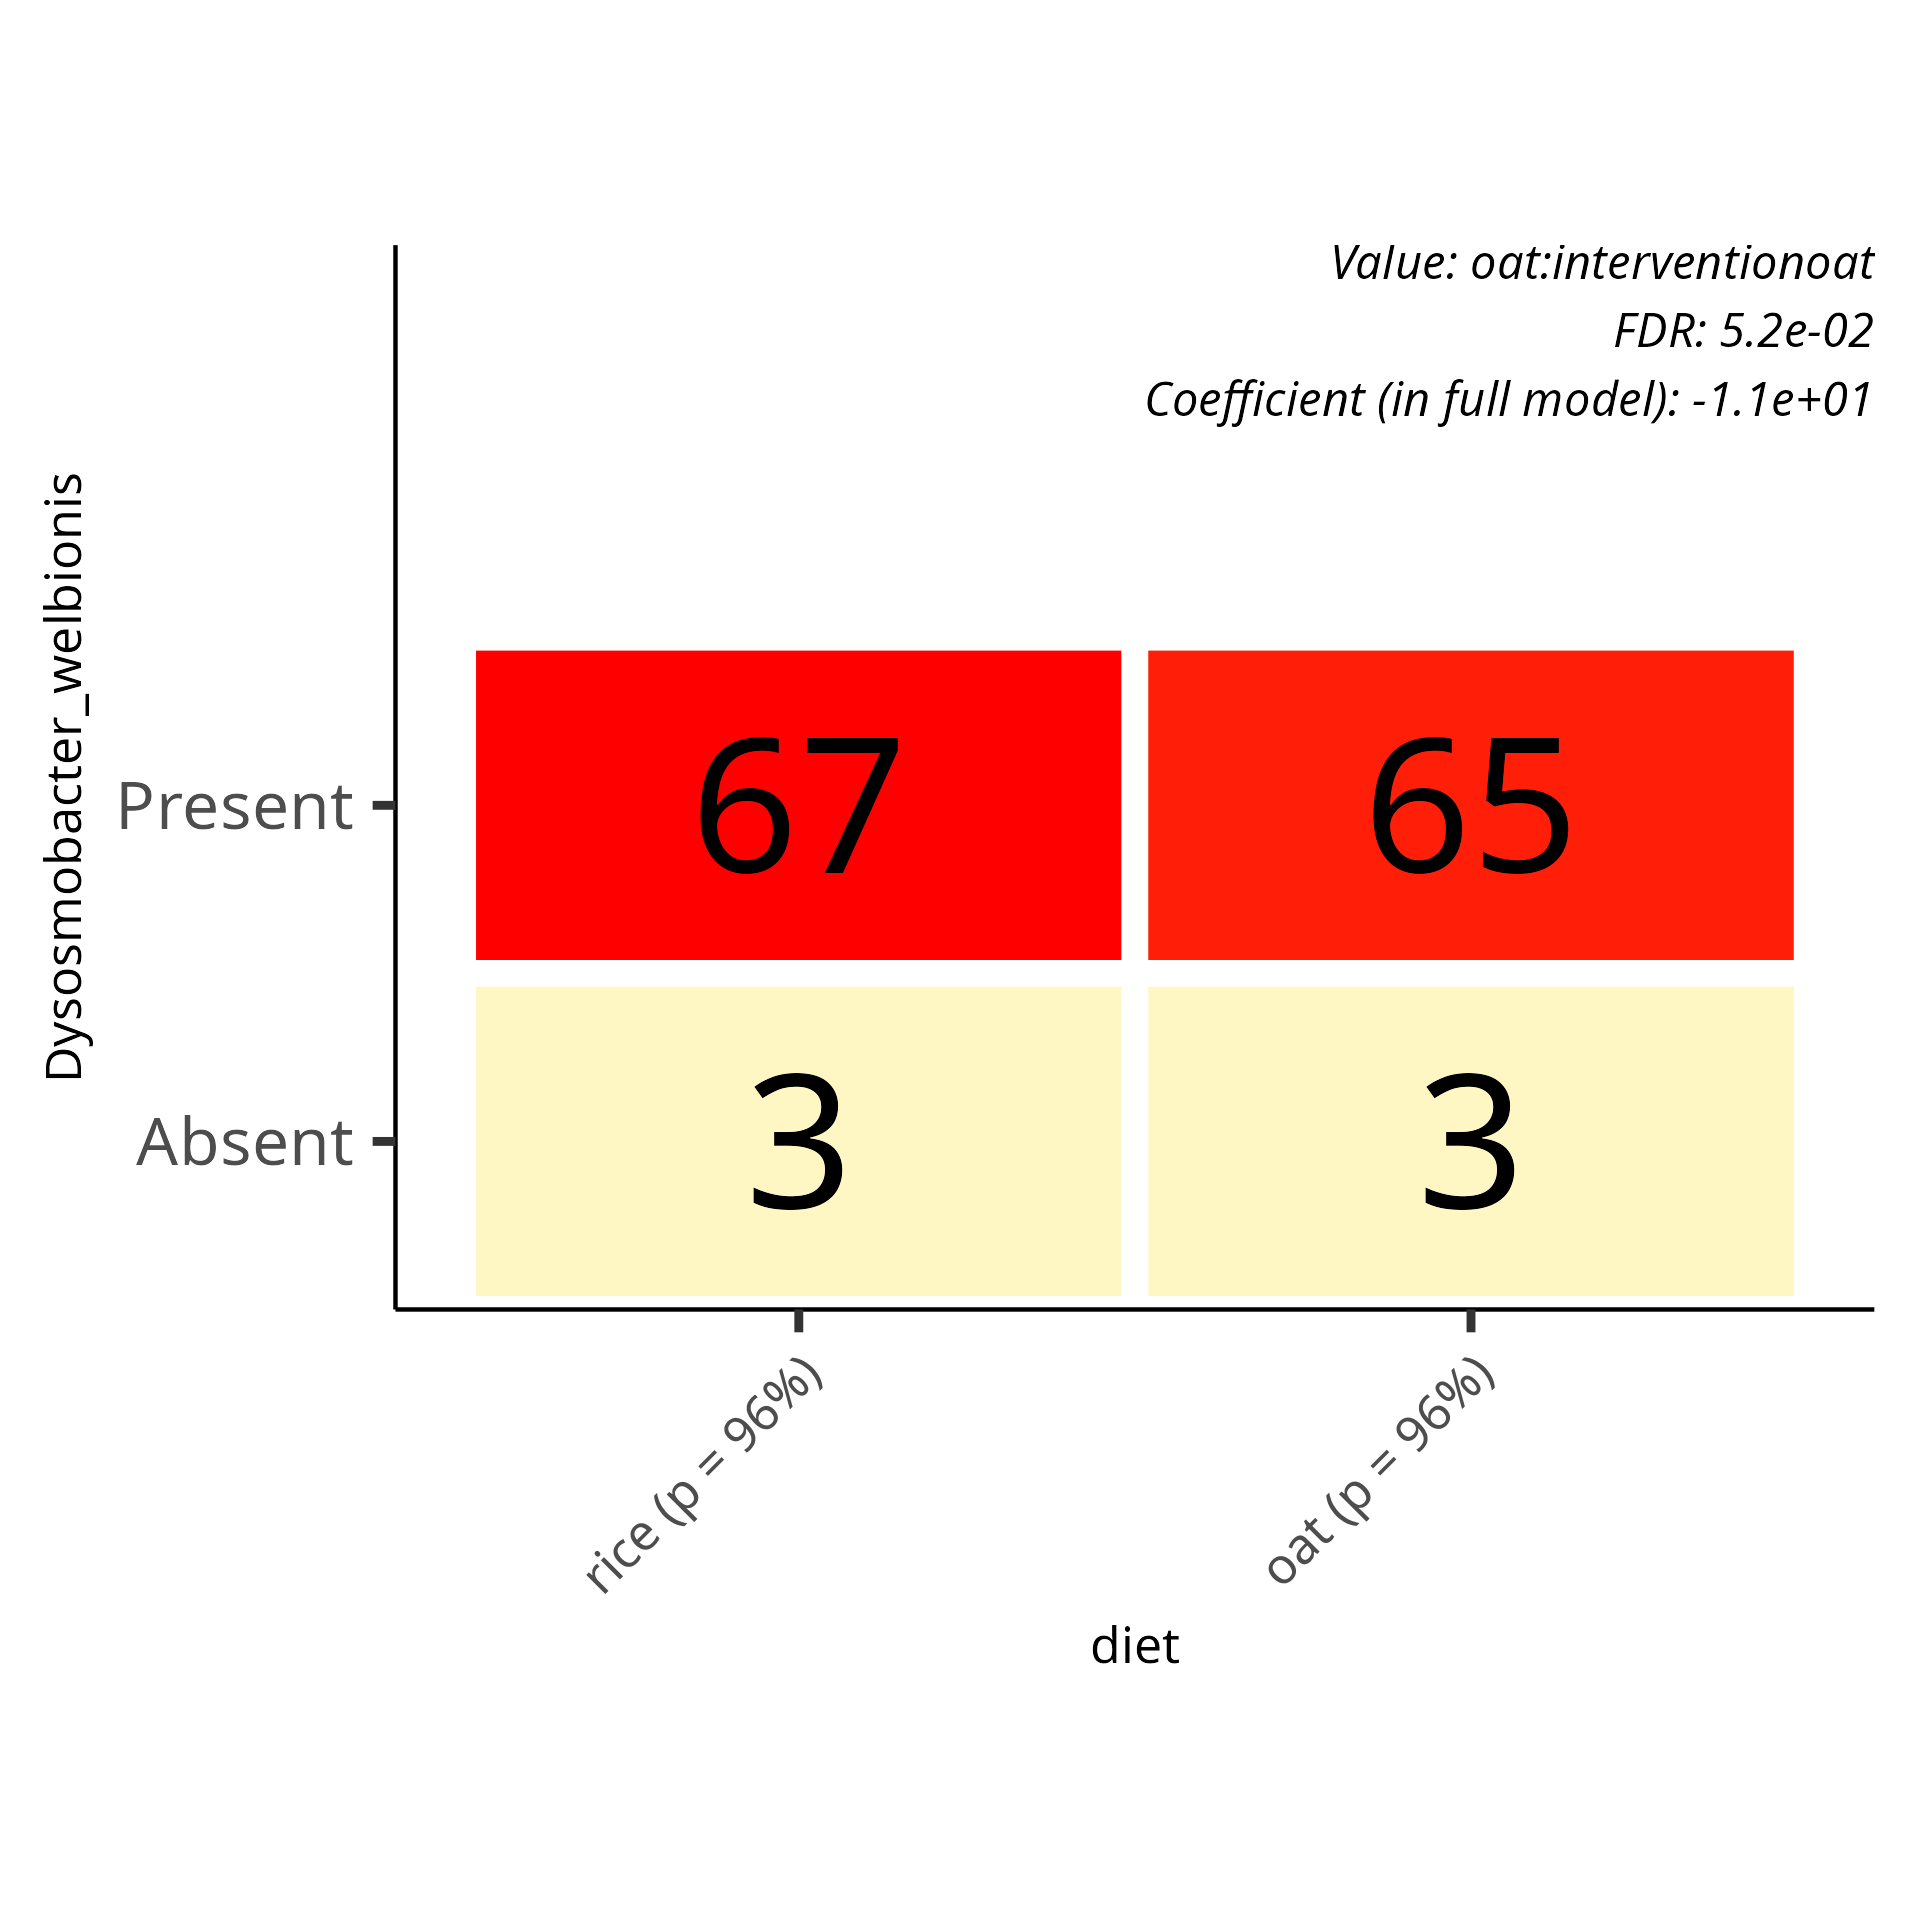
\includegraphics{../../output/daa/daa_taxa/species/figures/association_plots/diet/logistic/diet_Dysosmobacter_welbionis_logistic.png}\\
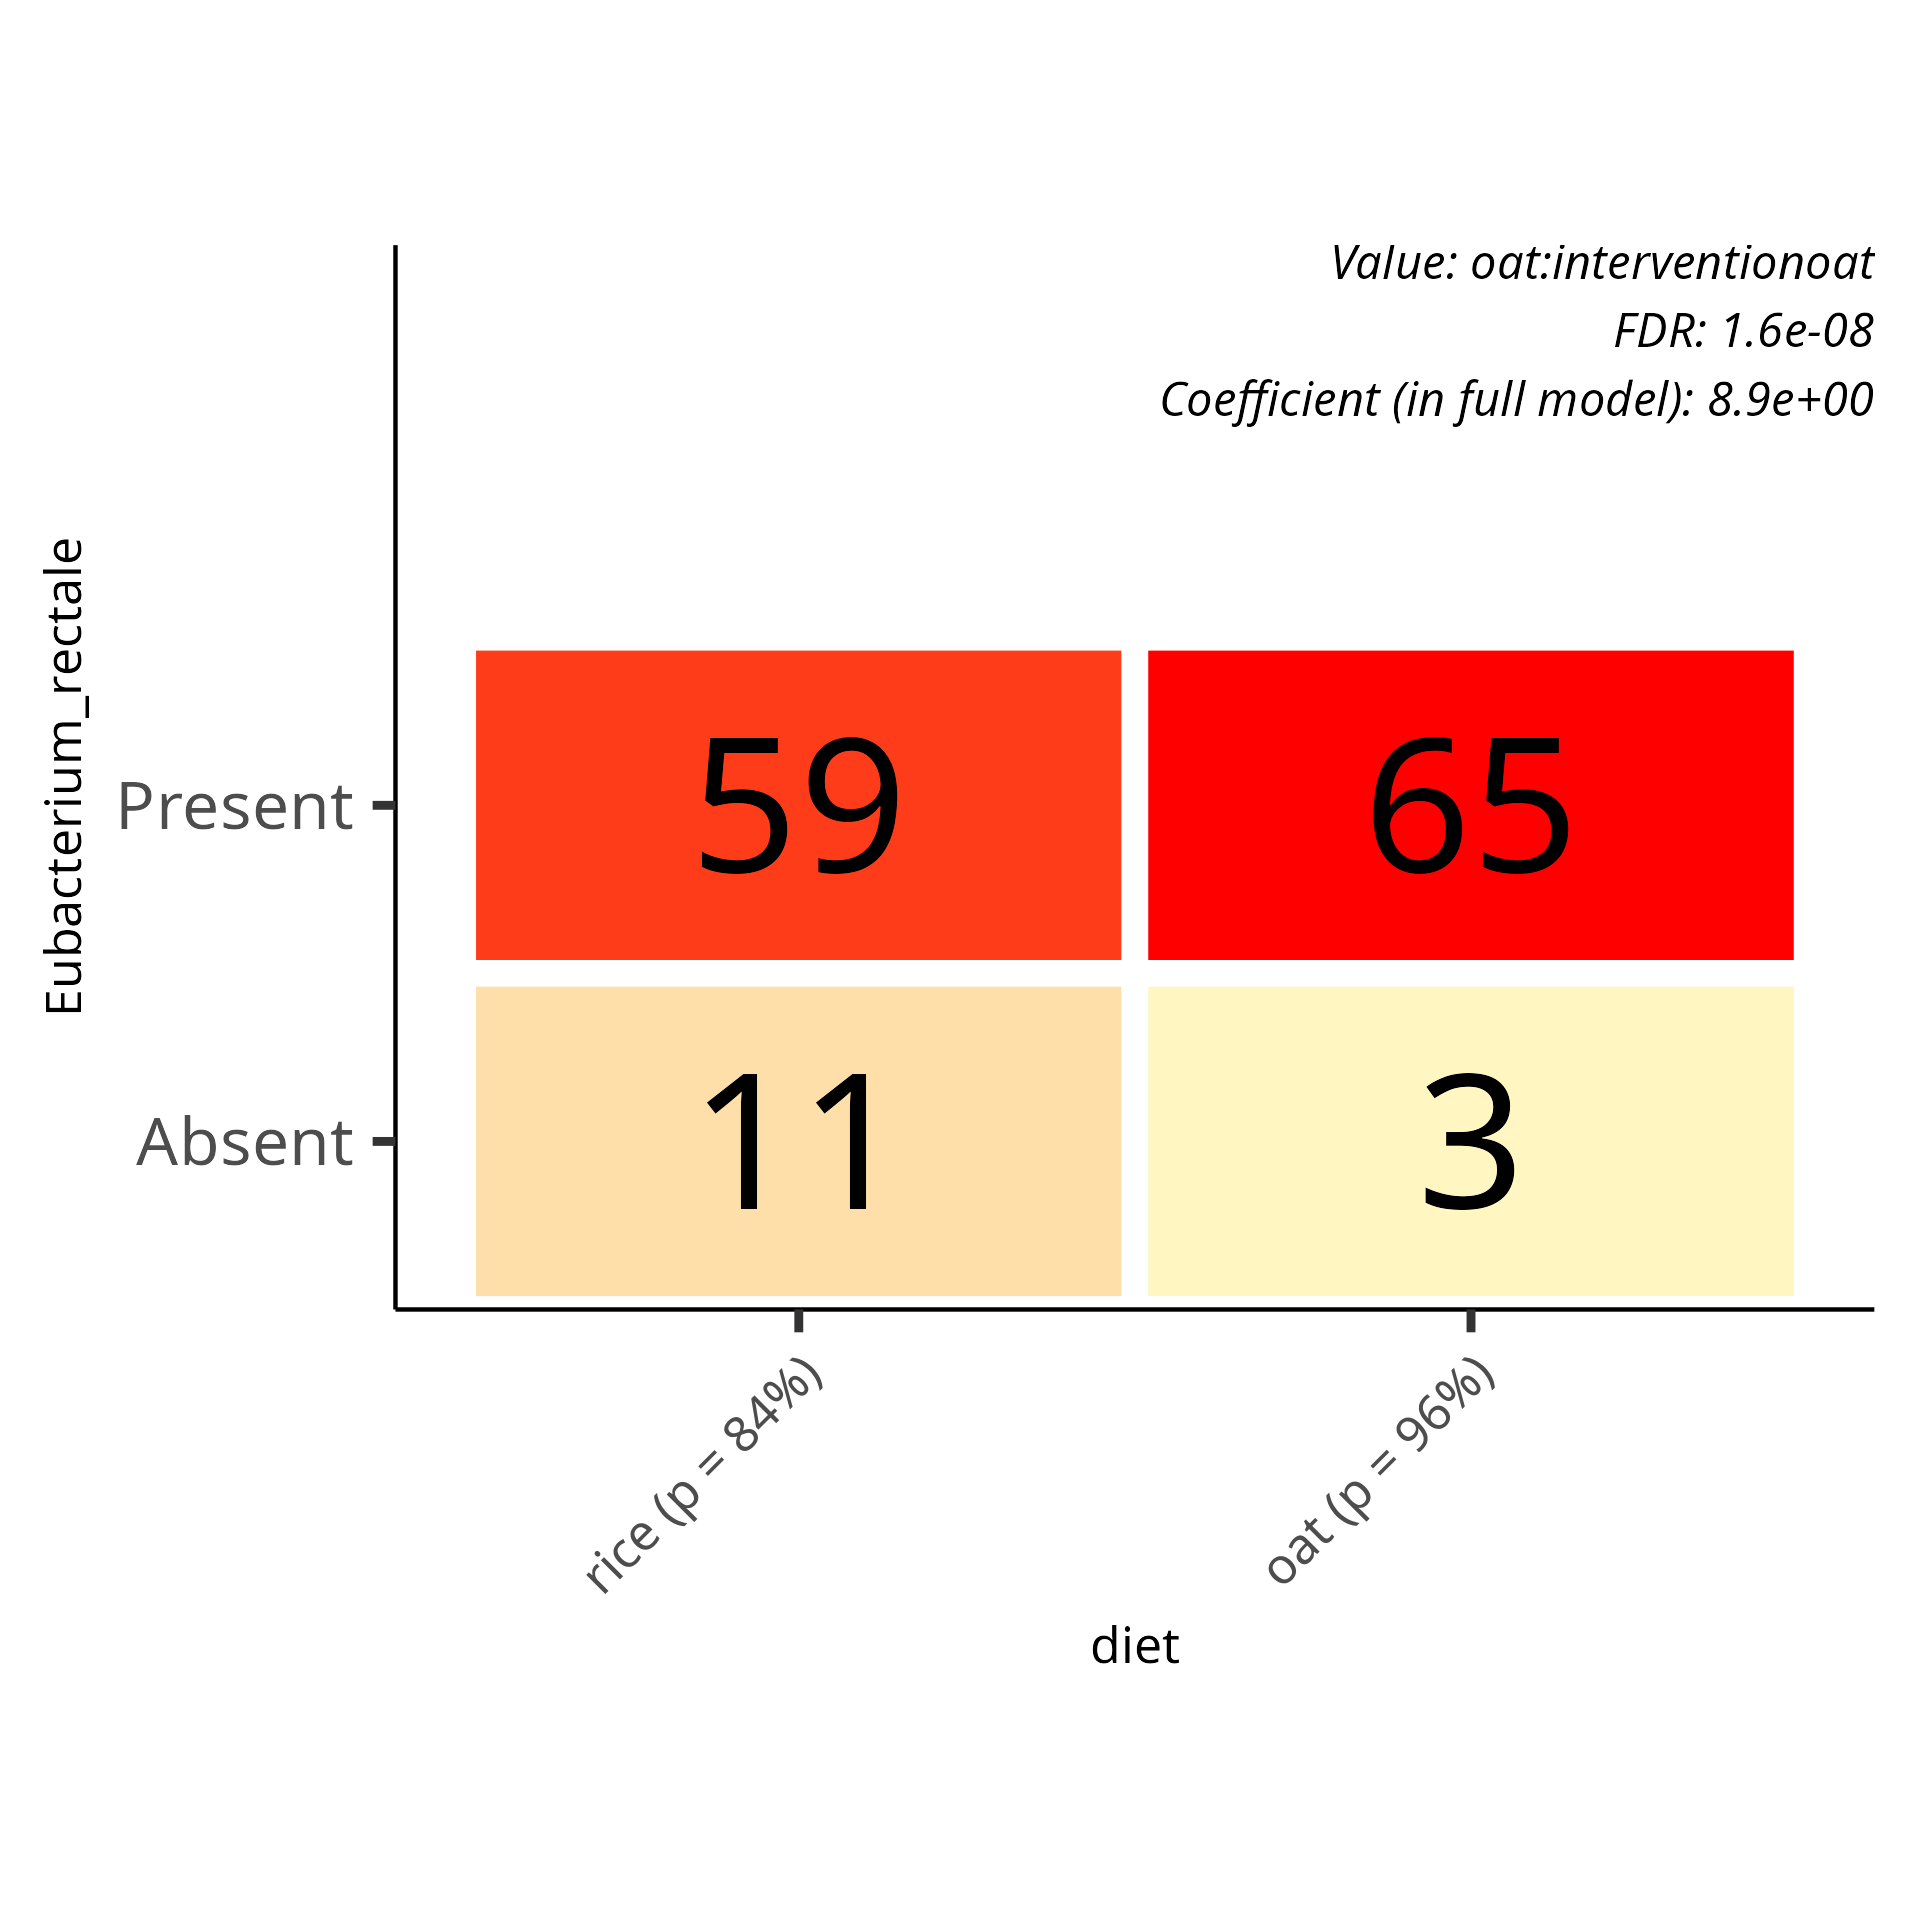
\includegraphics{../../output/daa/daa_taxa/species/figures/association_plots/diet/logistic/diet_Eubacterium_rectale_logistic.png}\\
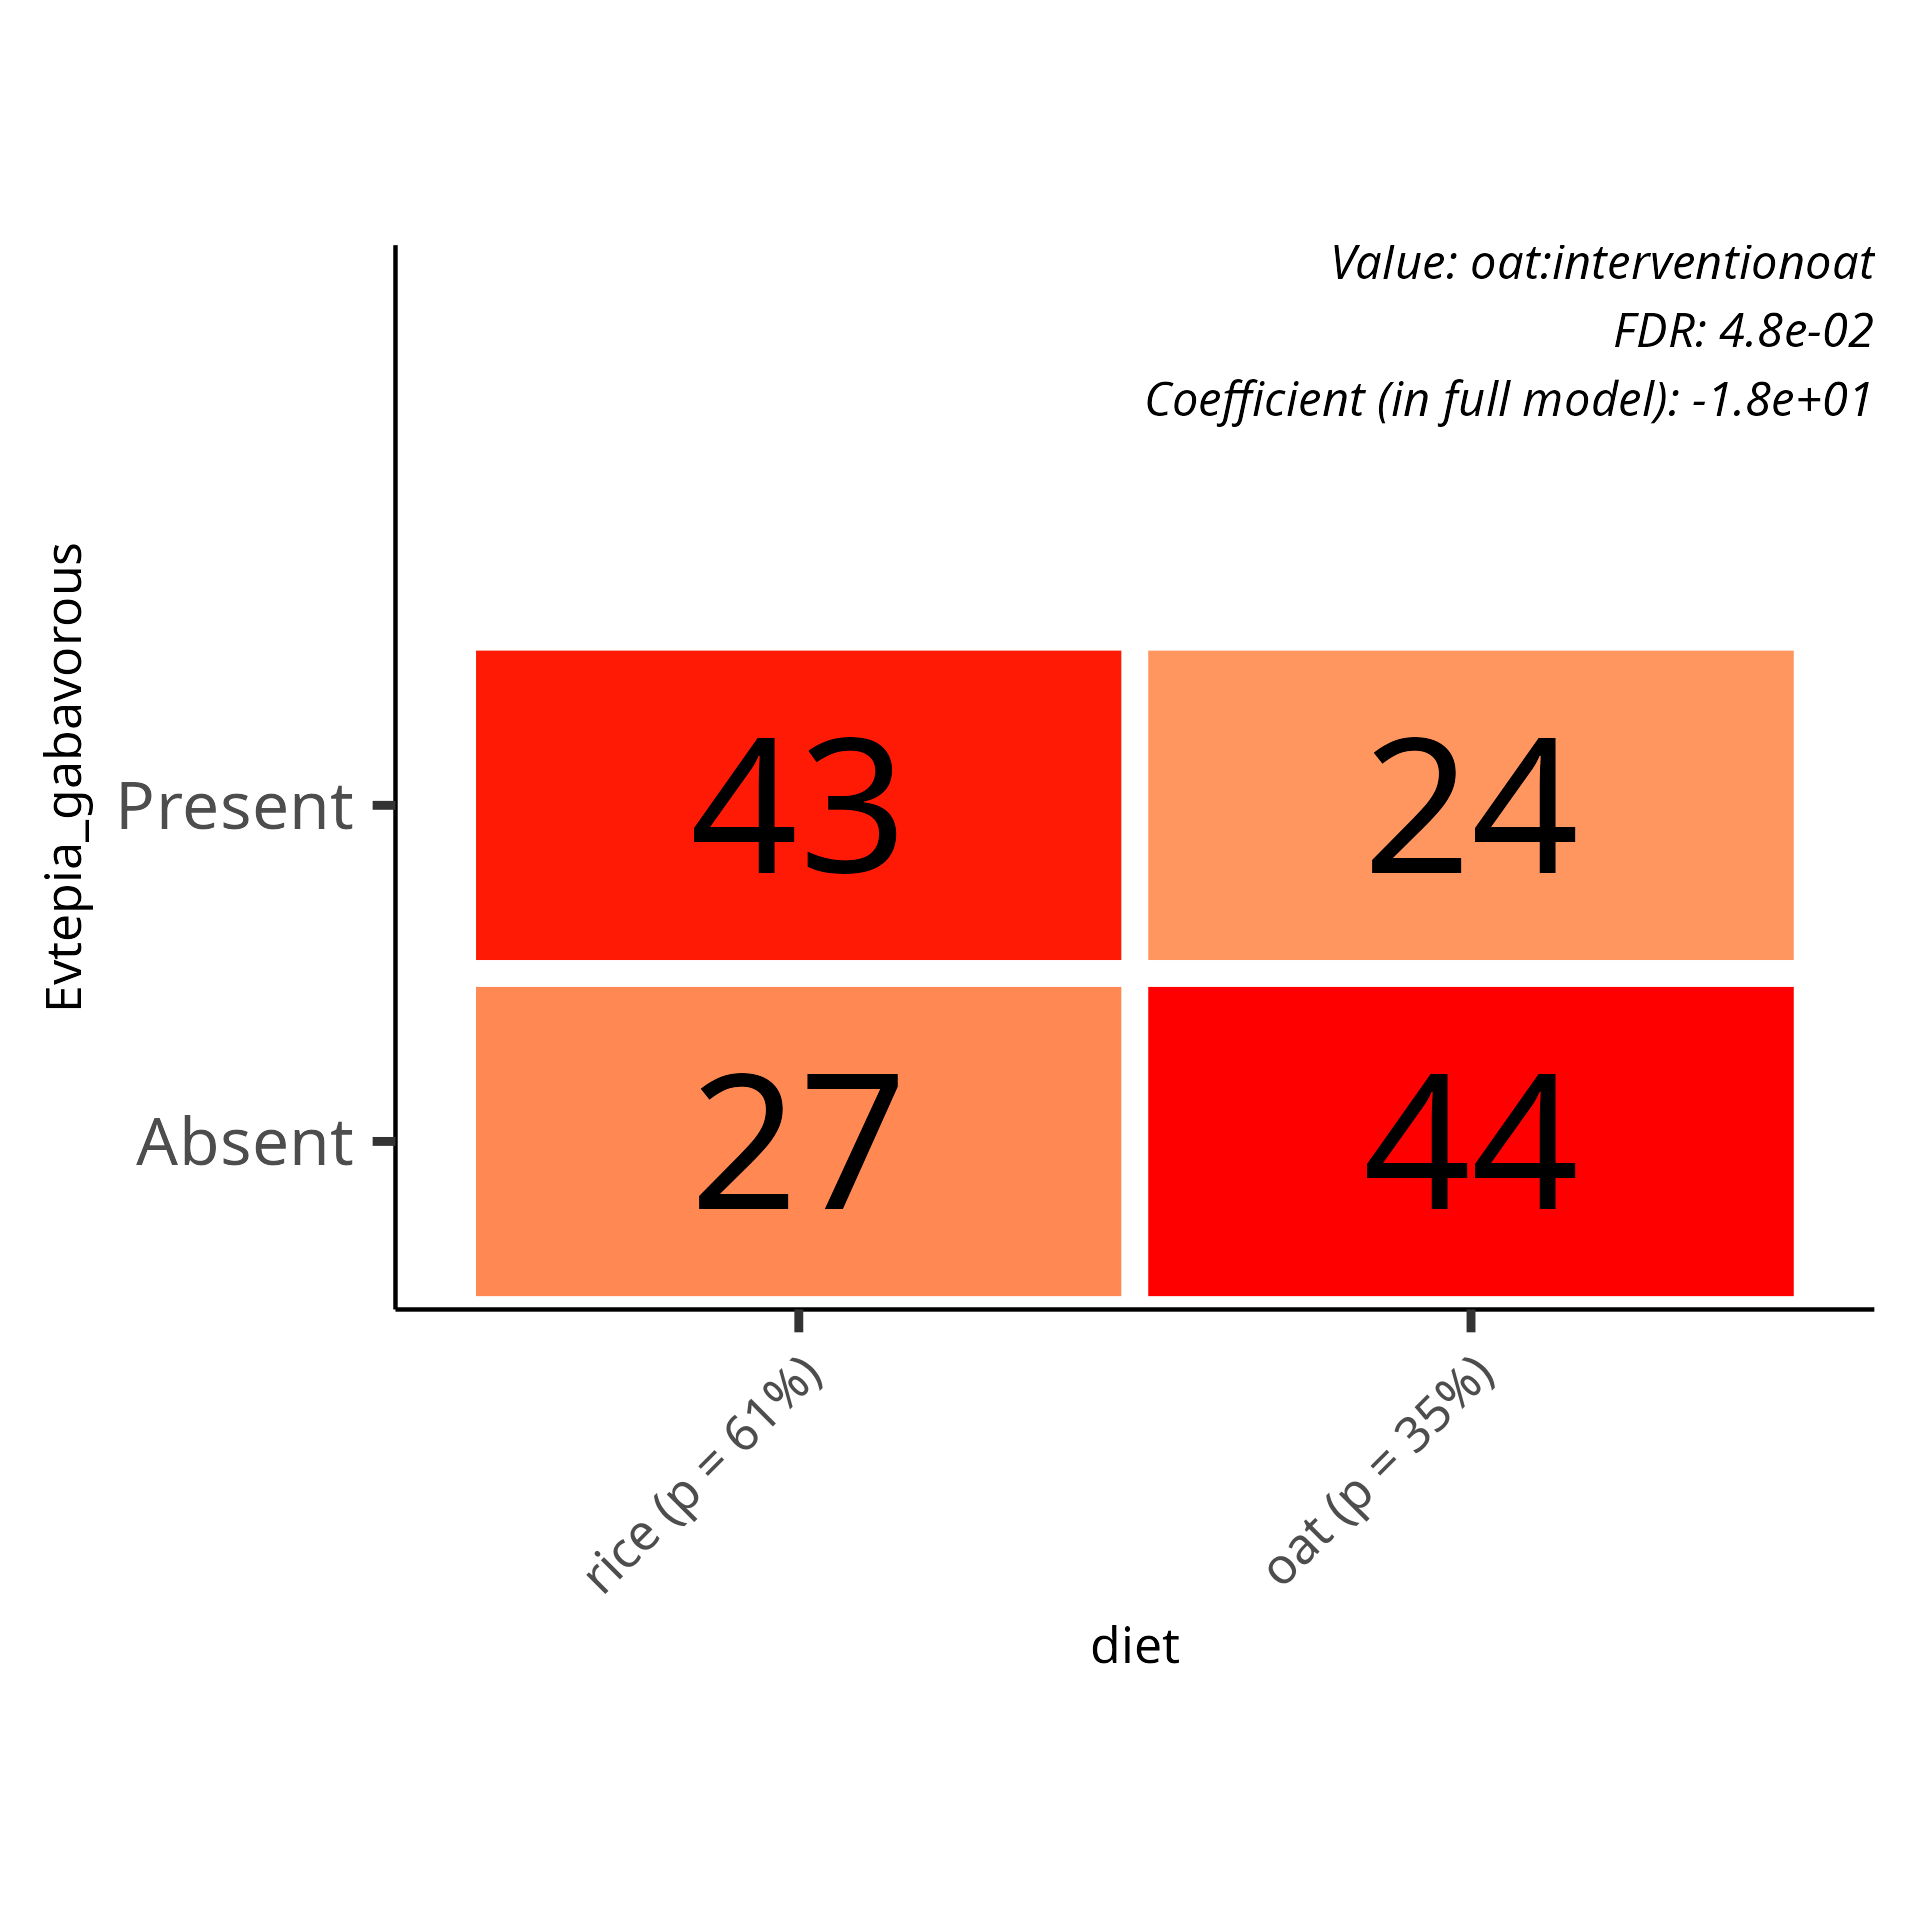
\includegraphics{../../output/daa/daa_taxa/species/figures/association_plots/diet/logistic/diet_Evtepia_gabavorous_logistic.png}\\
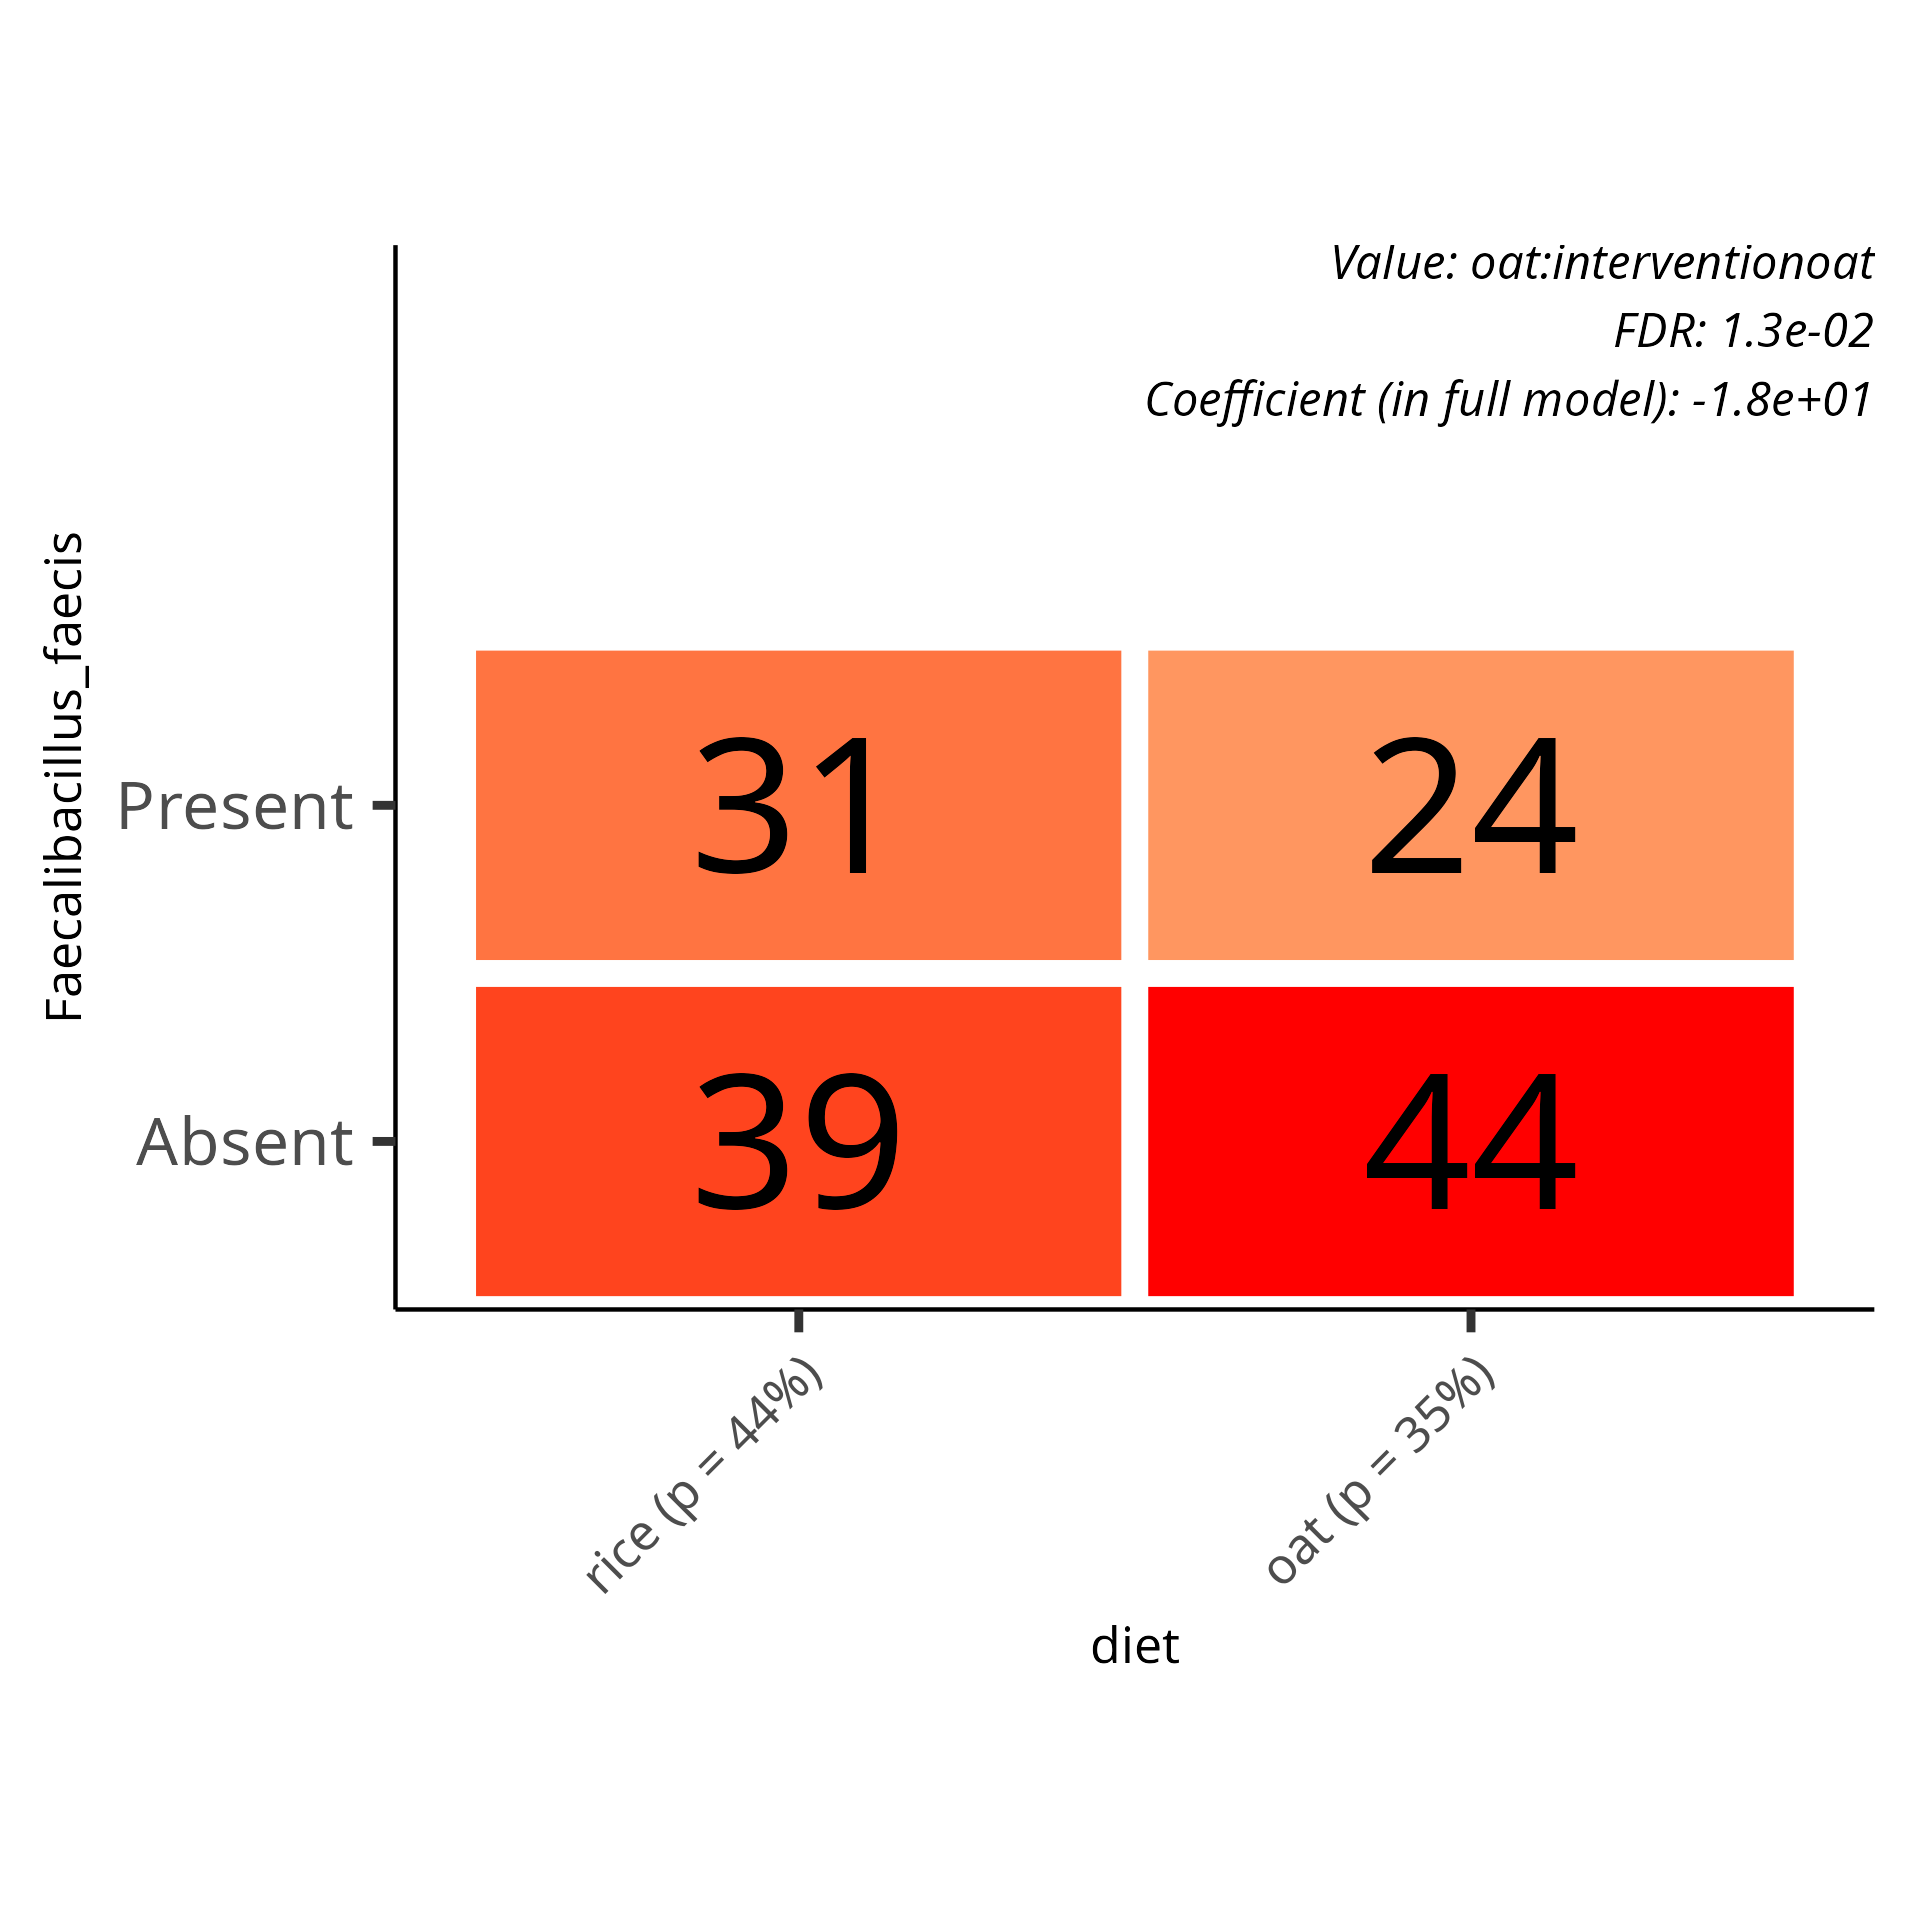
\includegraphics{../../output/daa/daa_taxa/species/figures/association_plots/diet/logistic/diet_Faecalibacillus_faecis_logistic.png}\\
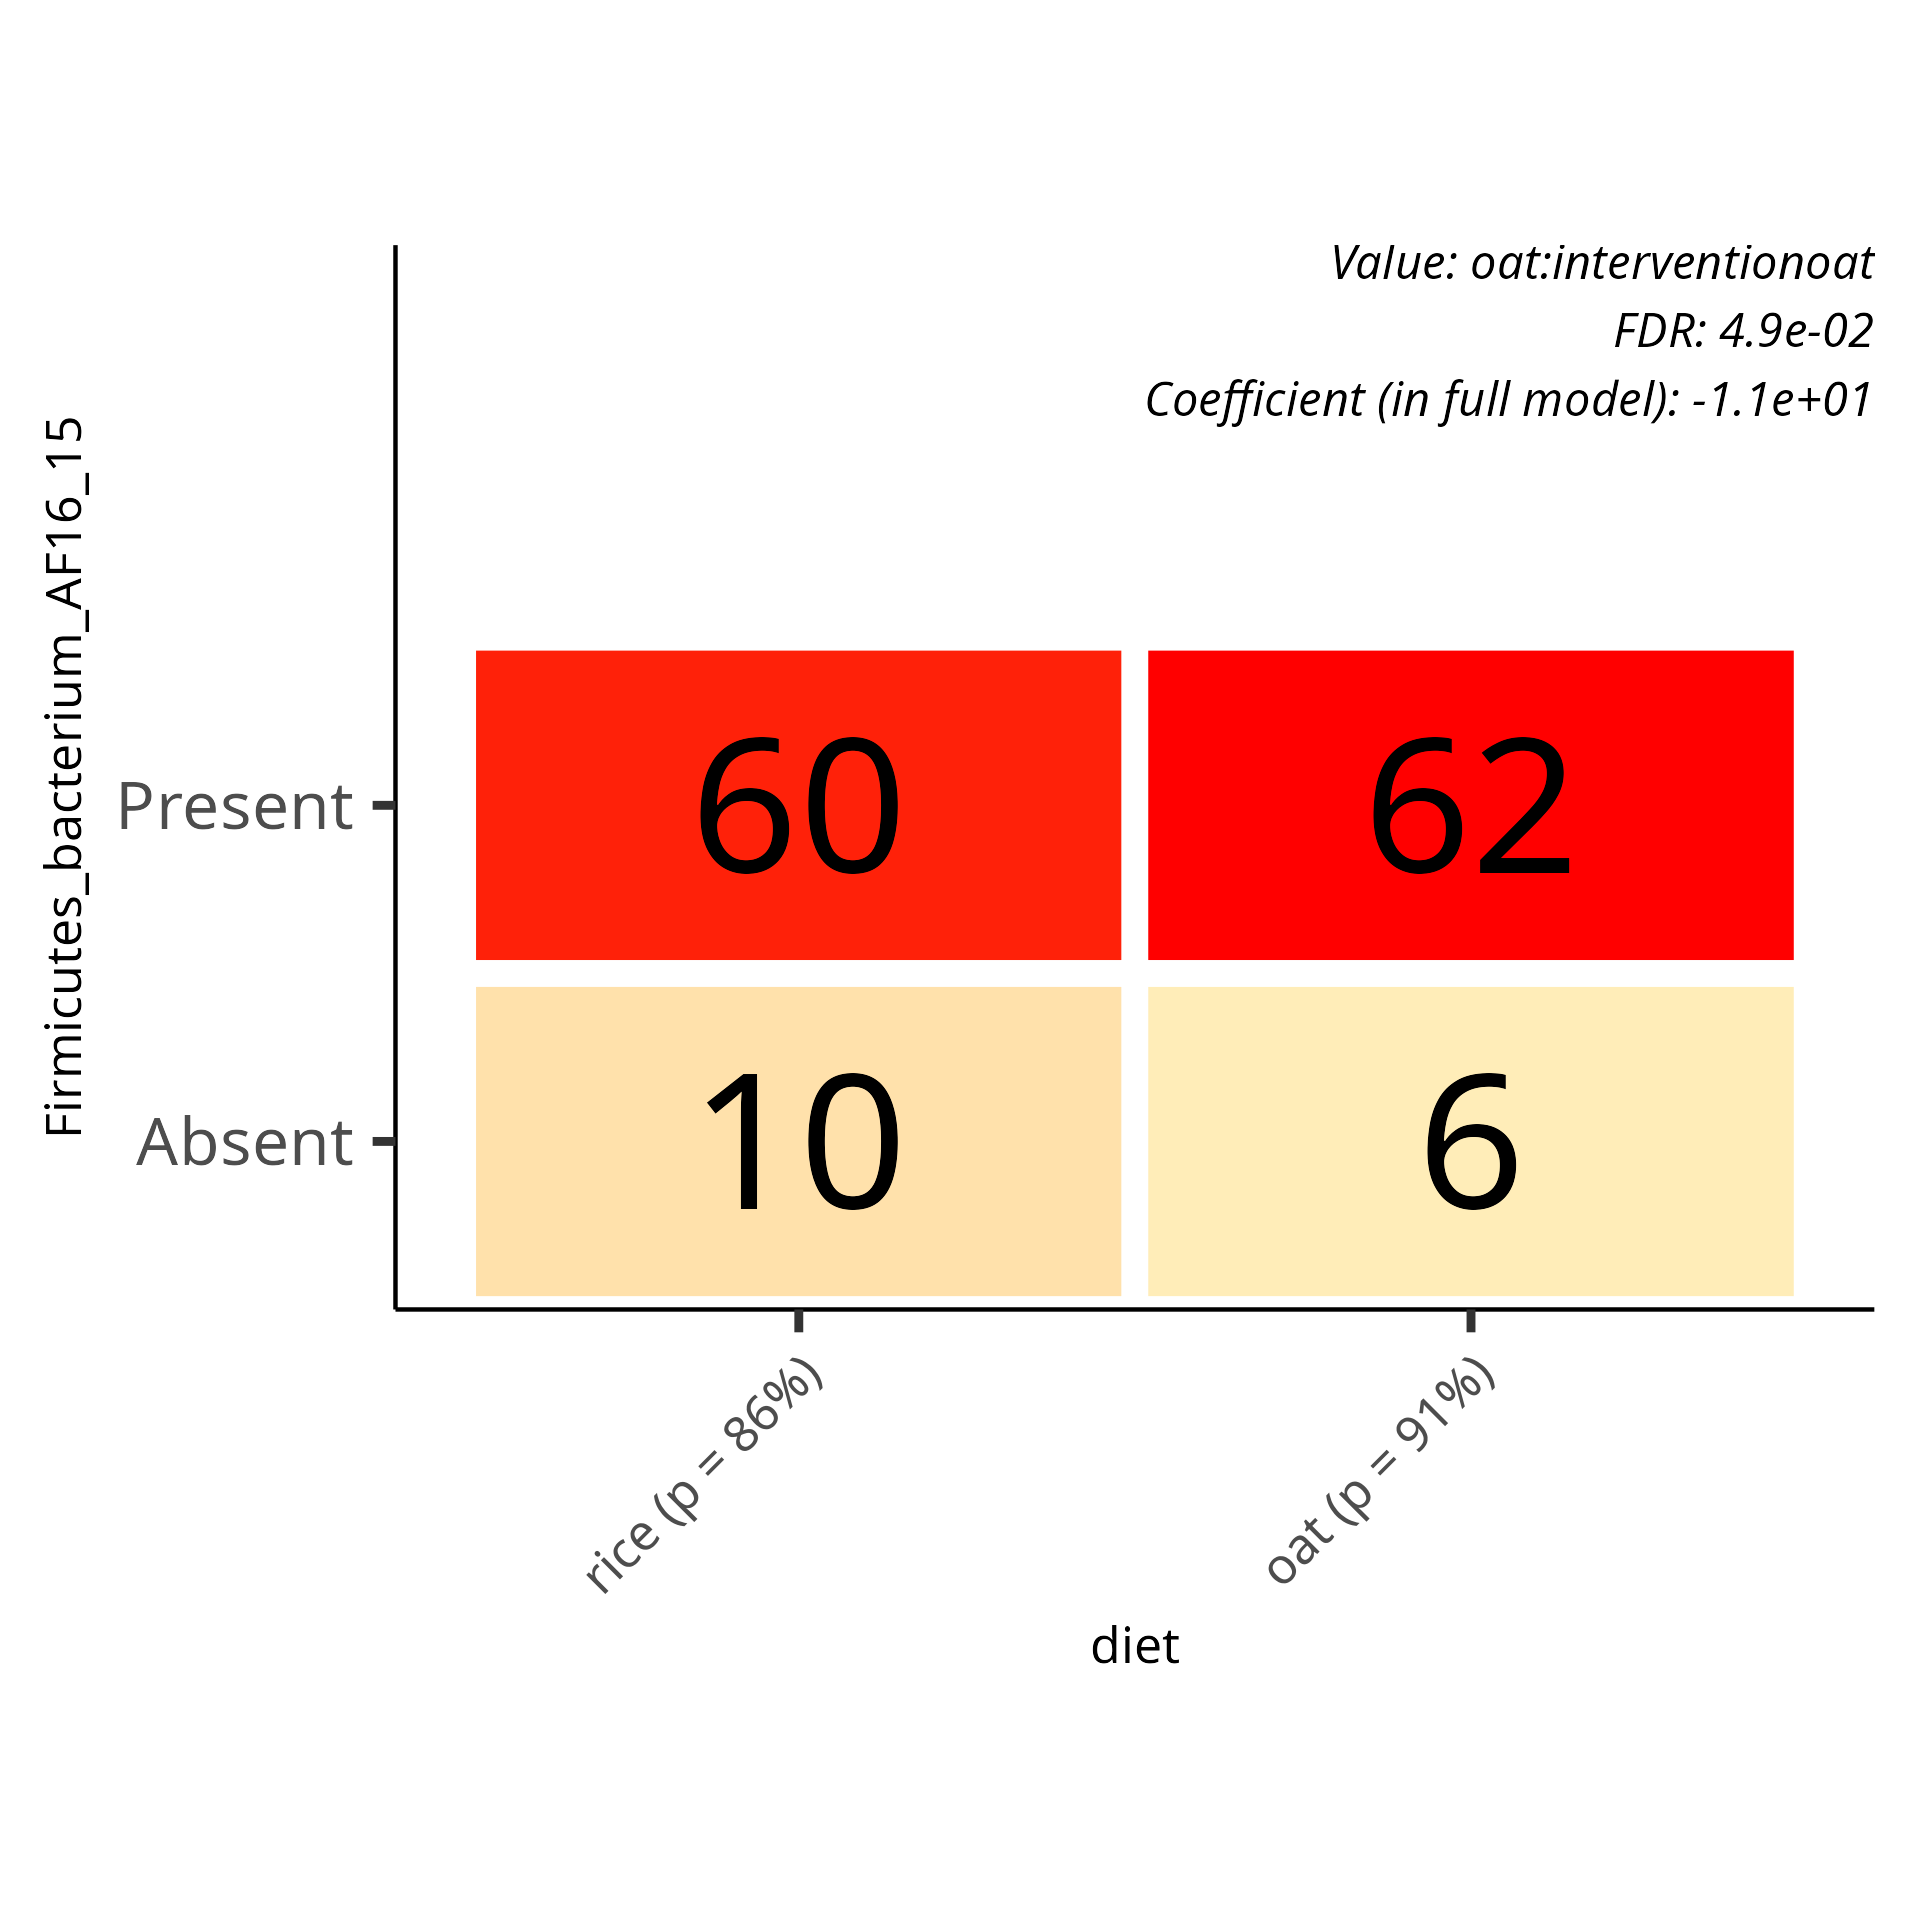
\includegraphics{../../output/daa/daa_taxa/species/figures/association_plots/diet/logistic/diet_Firmicutes_bacterium_AF16_15_logistic.png}\\
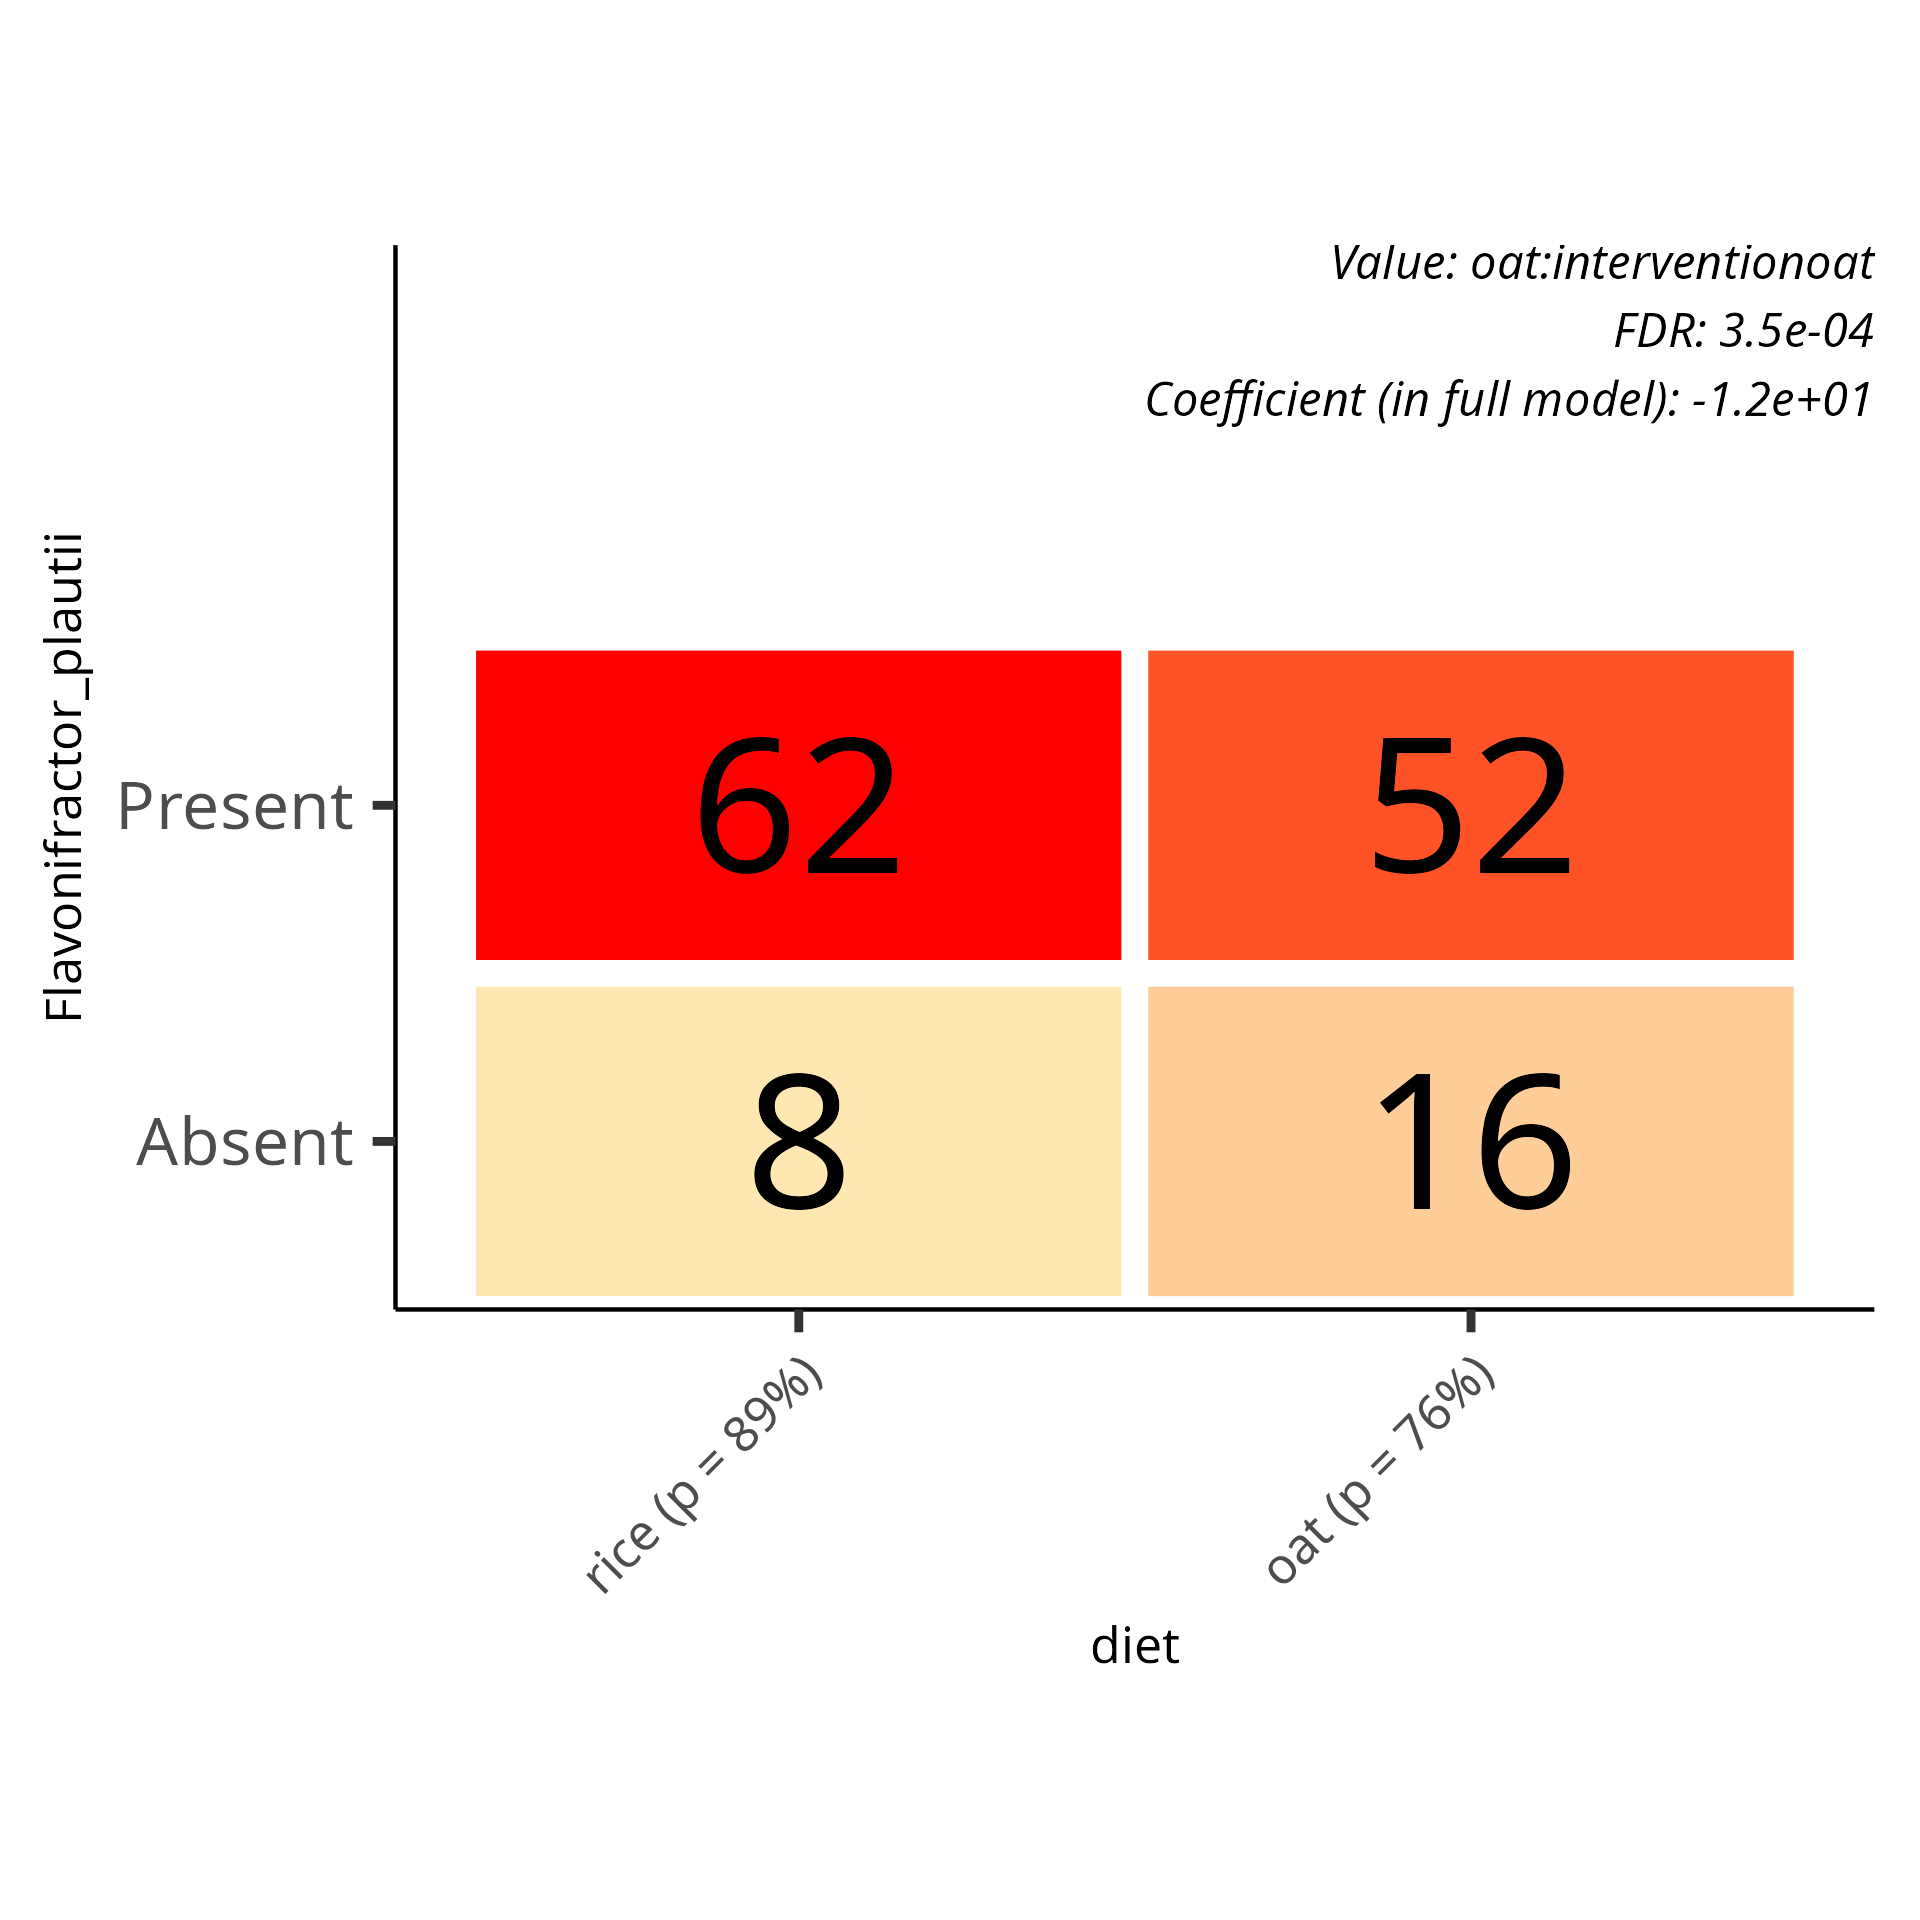
\includegraphics{../../output/daa/daa_taxa/species/figures/association_plots/diet/logistic/diet_Flavonifractor_plautii_logistic.png}\\
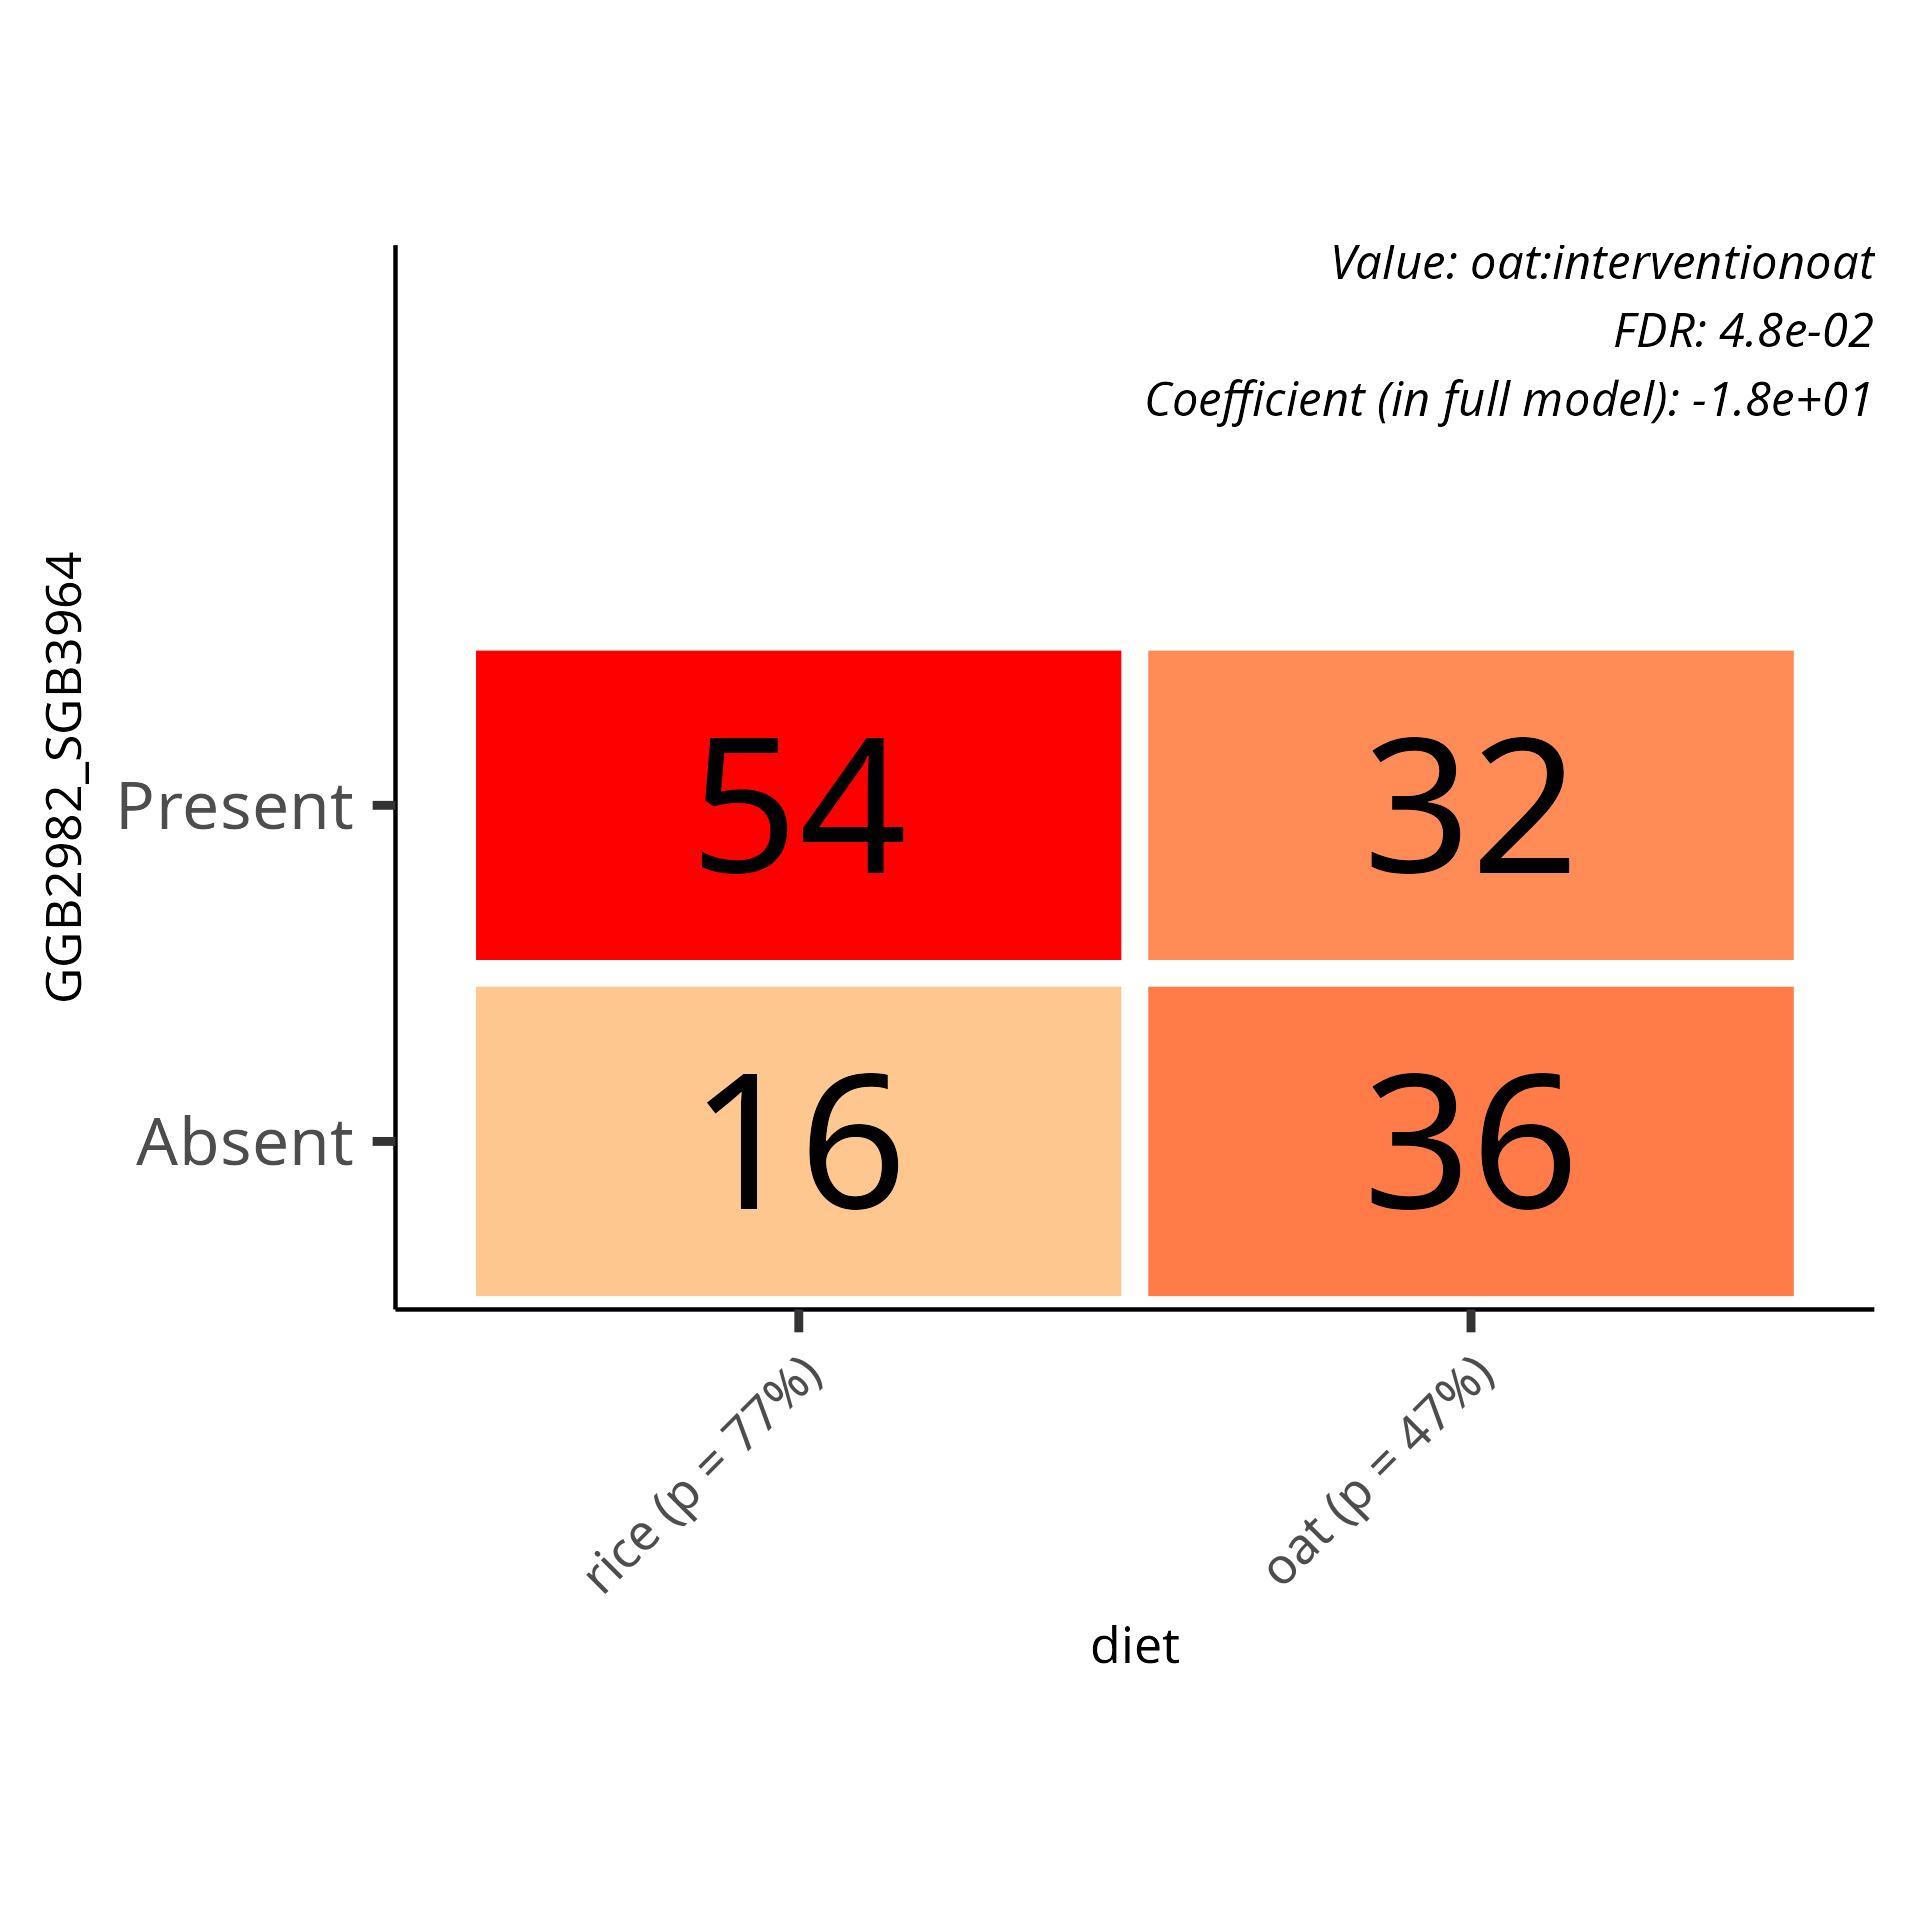
\includegraphics{../../output/daa/daa_taxa/species/figures/association_plots/diet/logistic/diet_GGB2982_SGB3964_logistic.png}\\
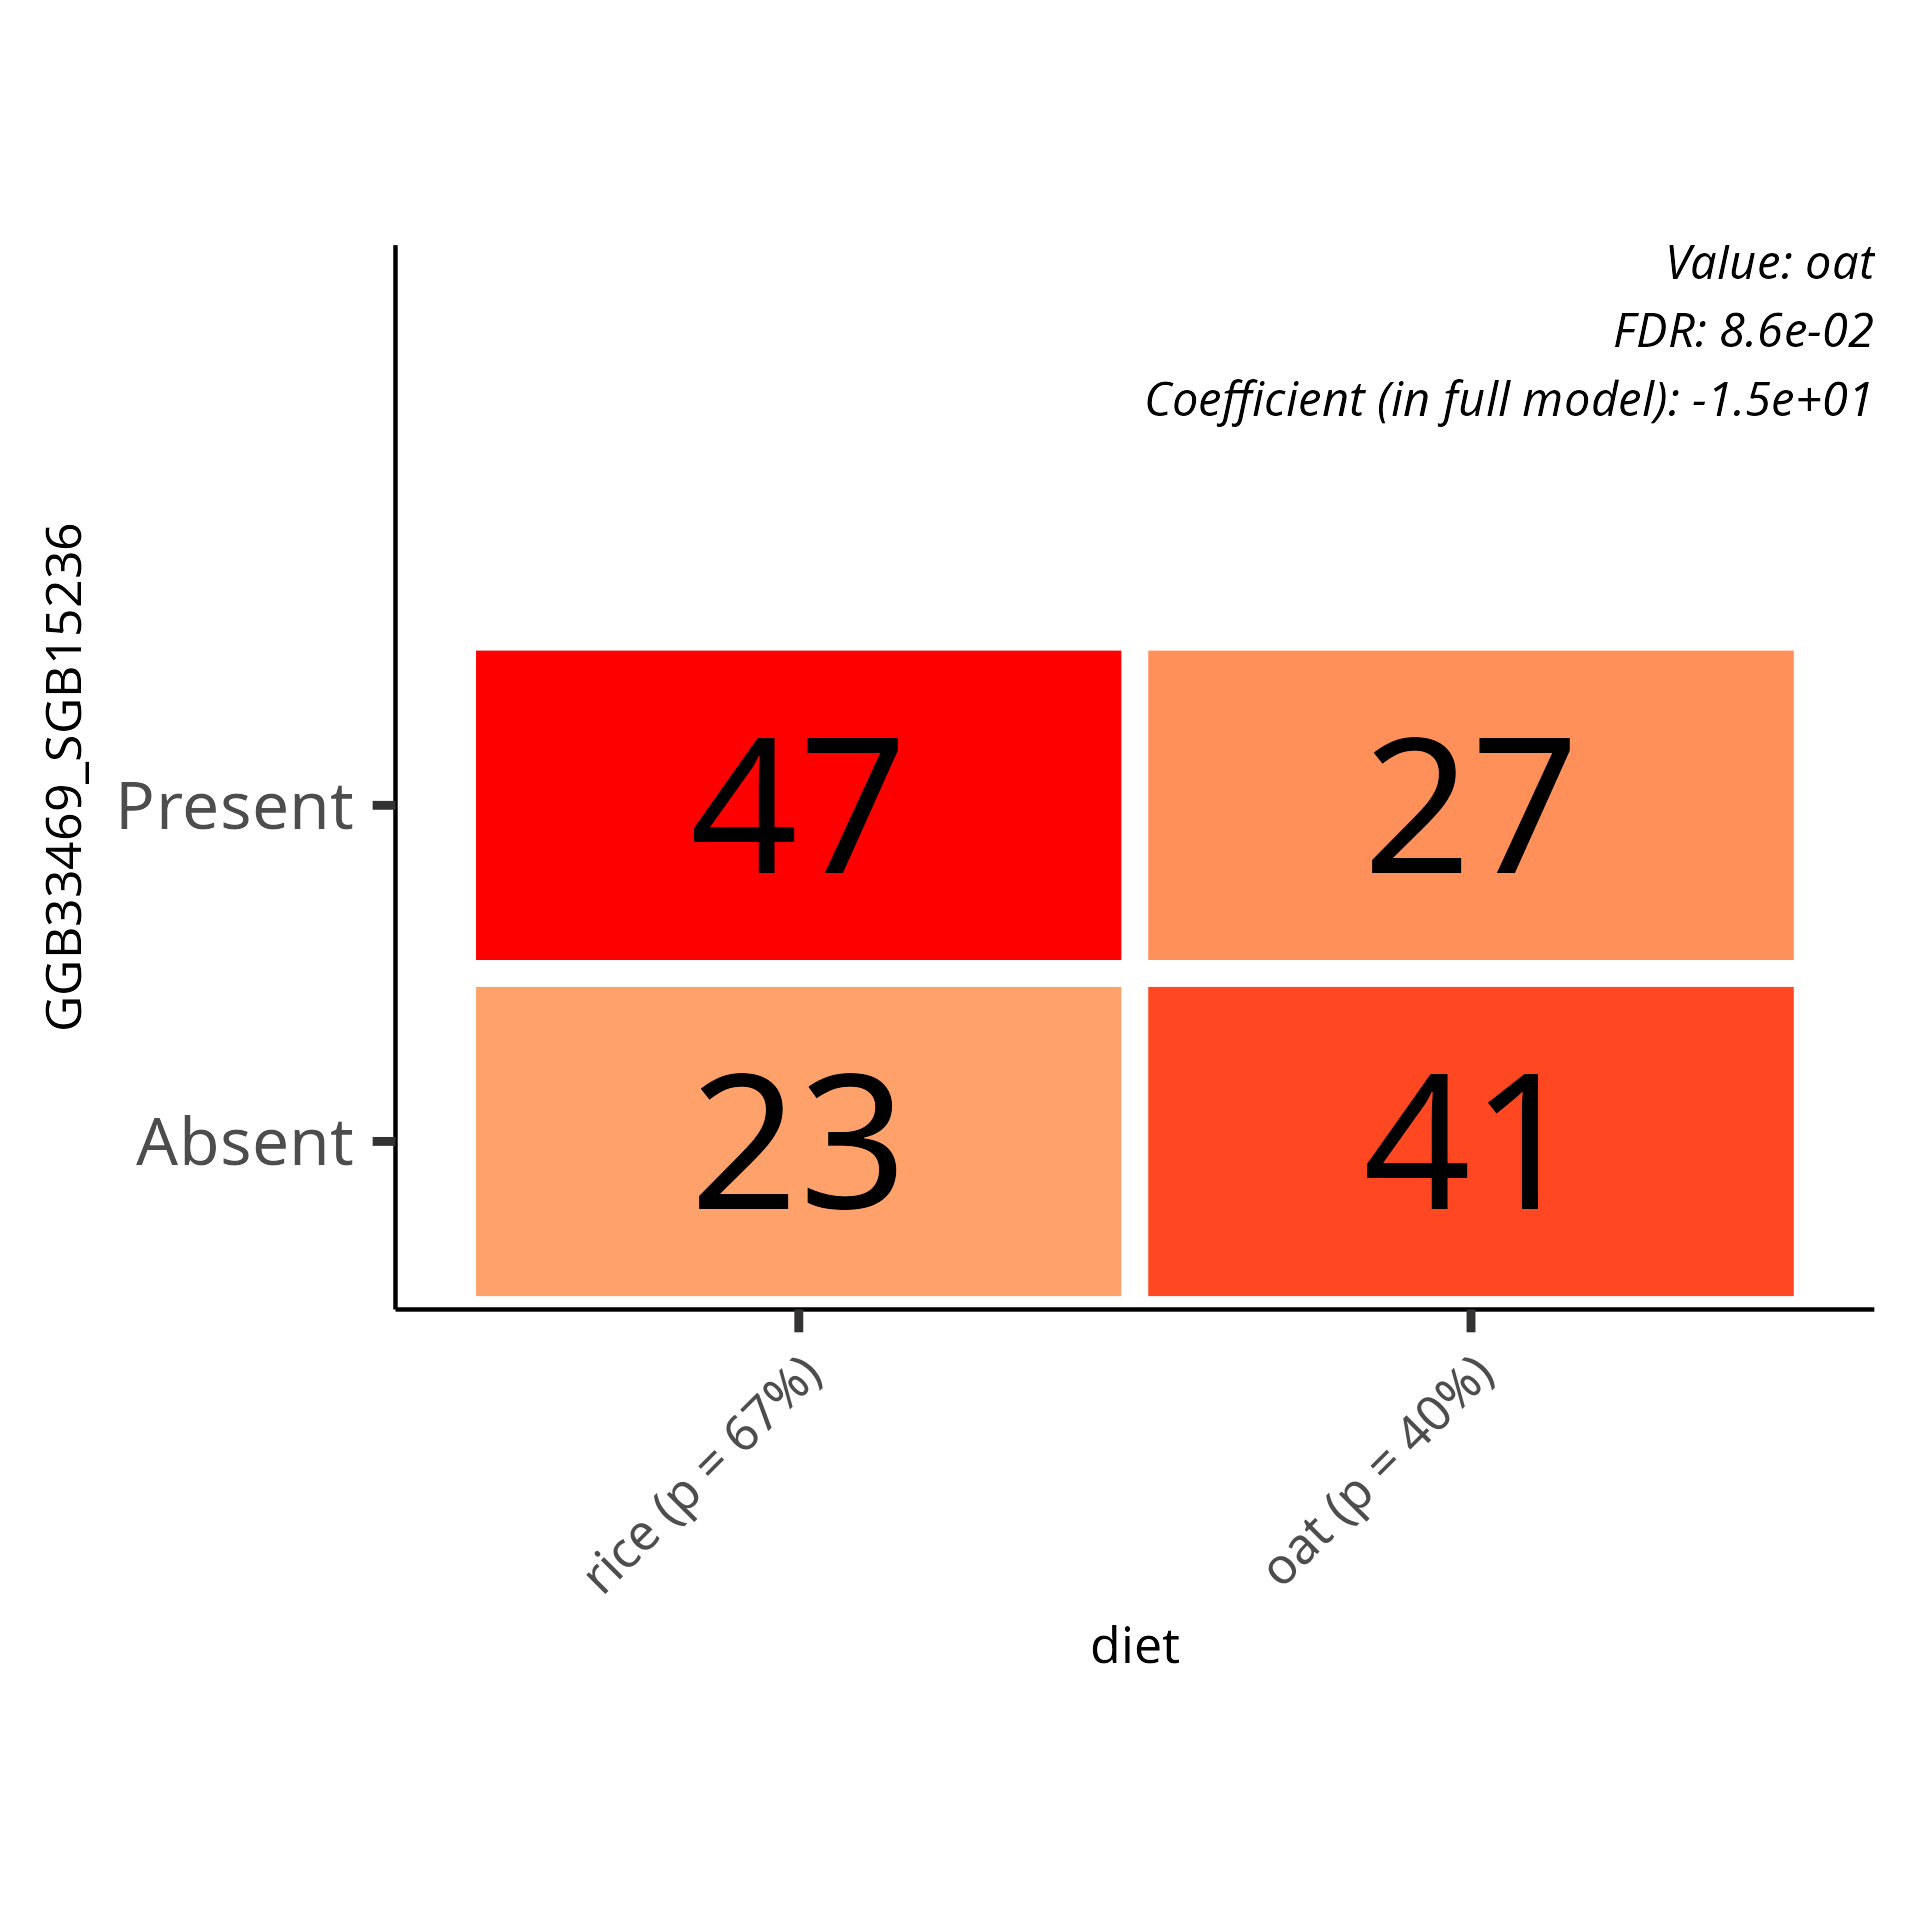
\includegraphics{../../output/daa/daa_taxa/species/figures/association_plots/diet/logistic/diet_GGB33469_SGB15236_logistic.png}\\
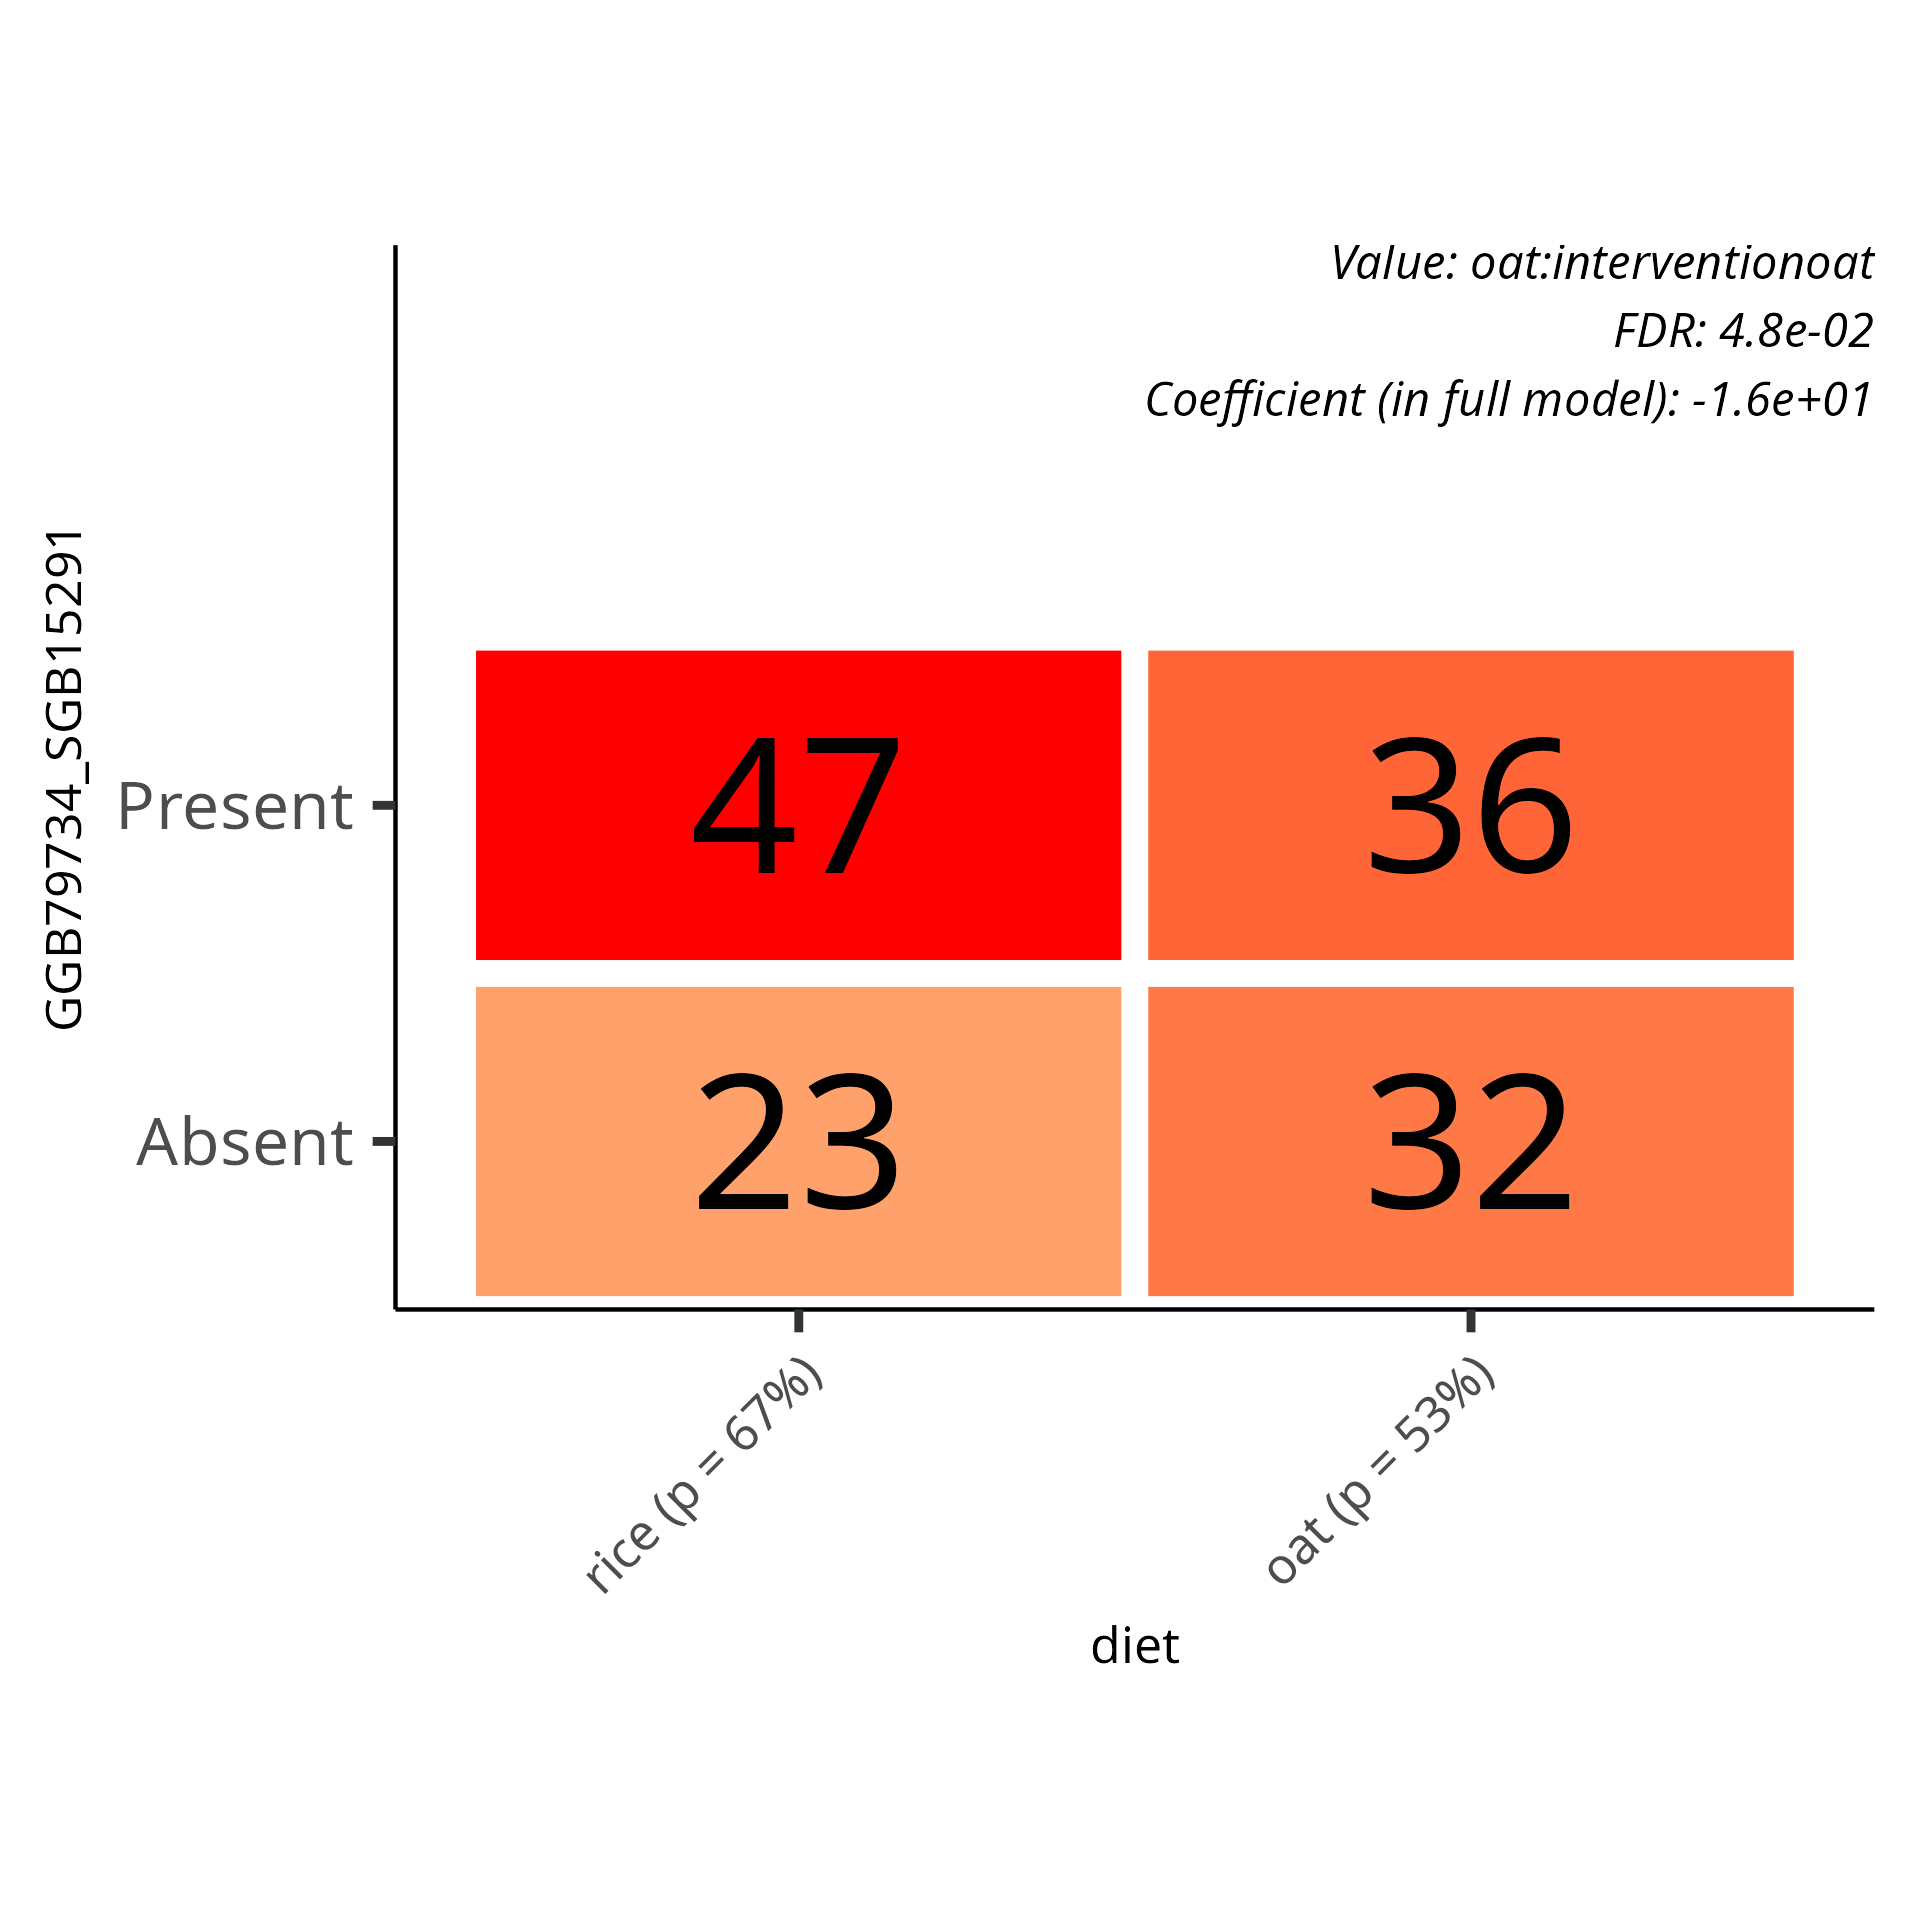
\includegraphics{../../output/daa/daa_taxa/species/figures/association_plots/diet/logistic/diet_GGB79734_SGB15291_logistic.png}\\
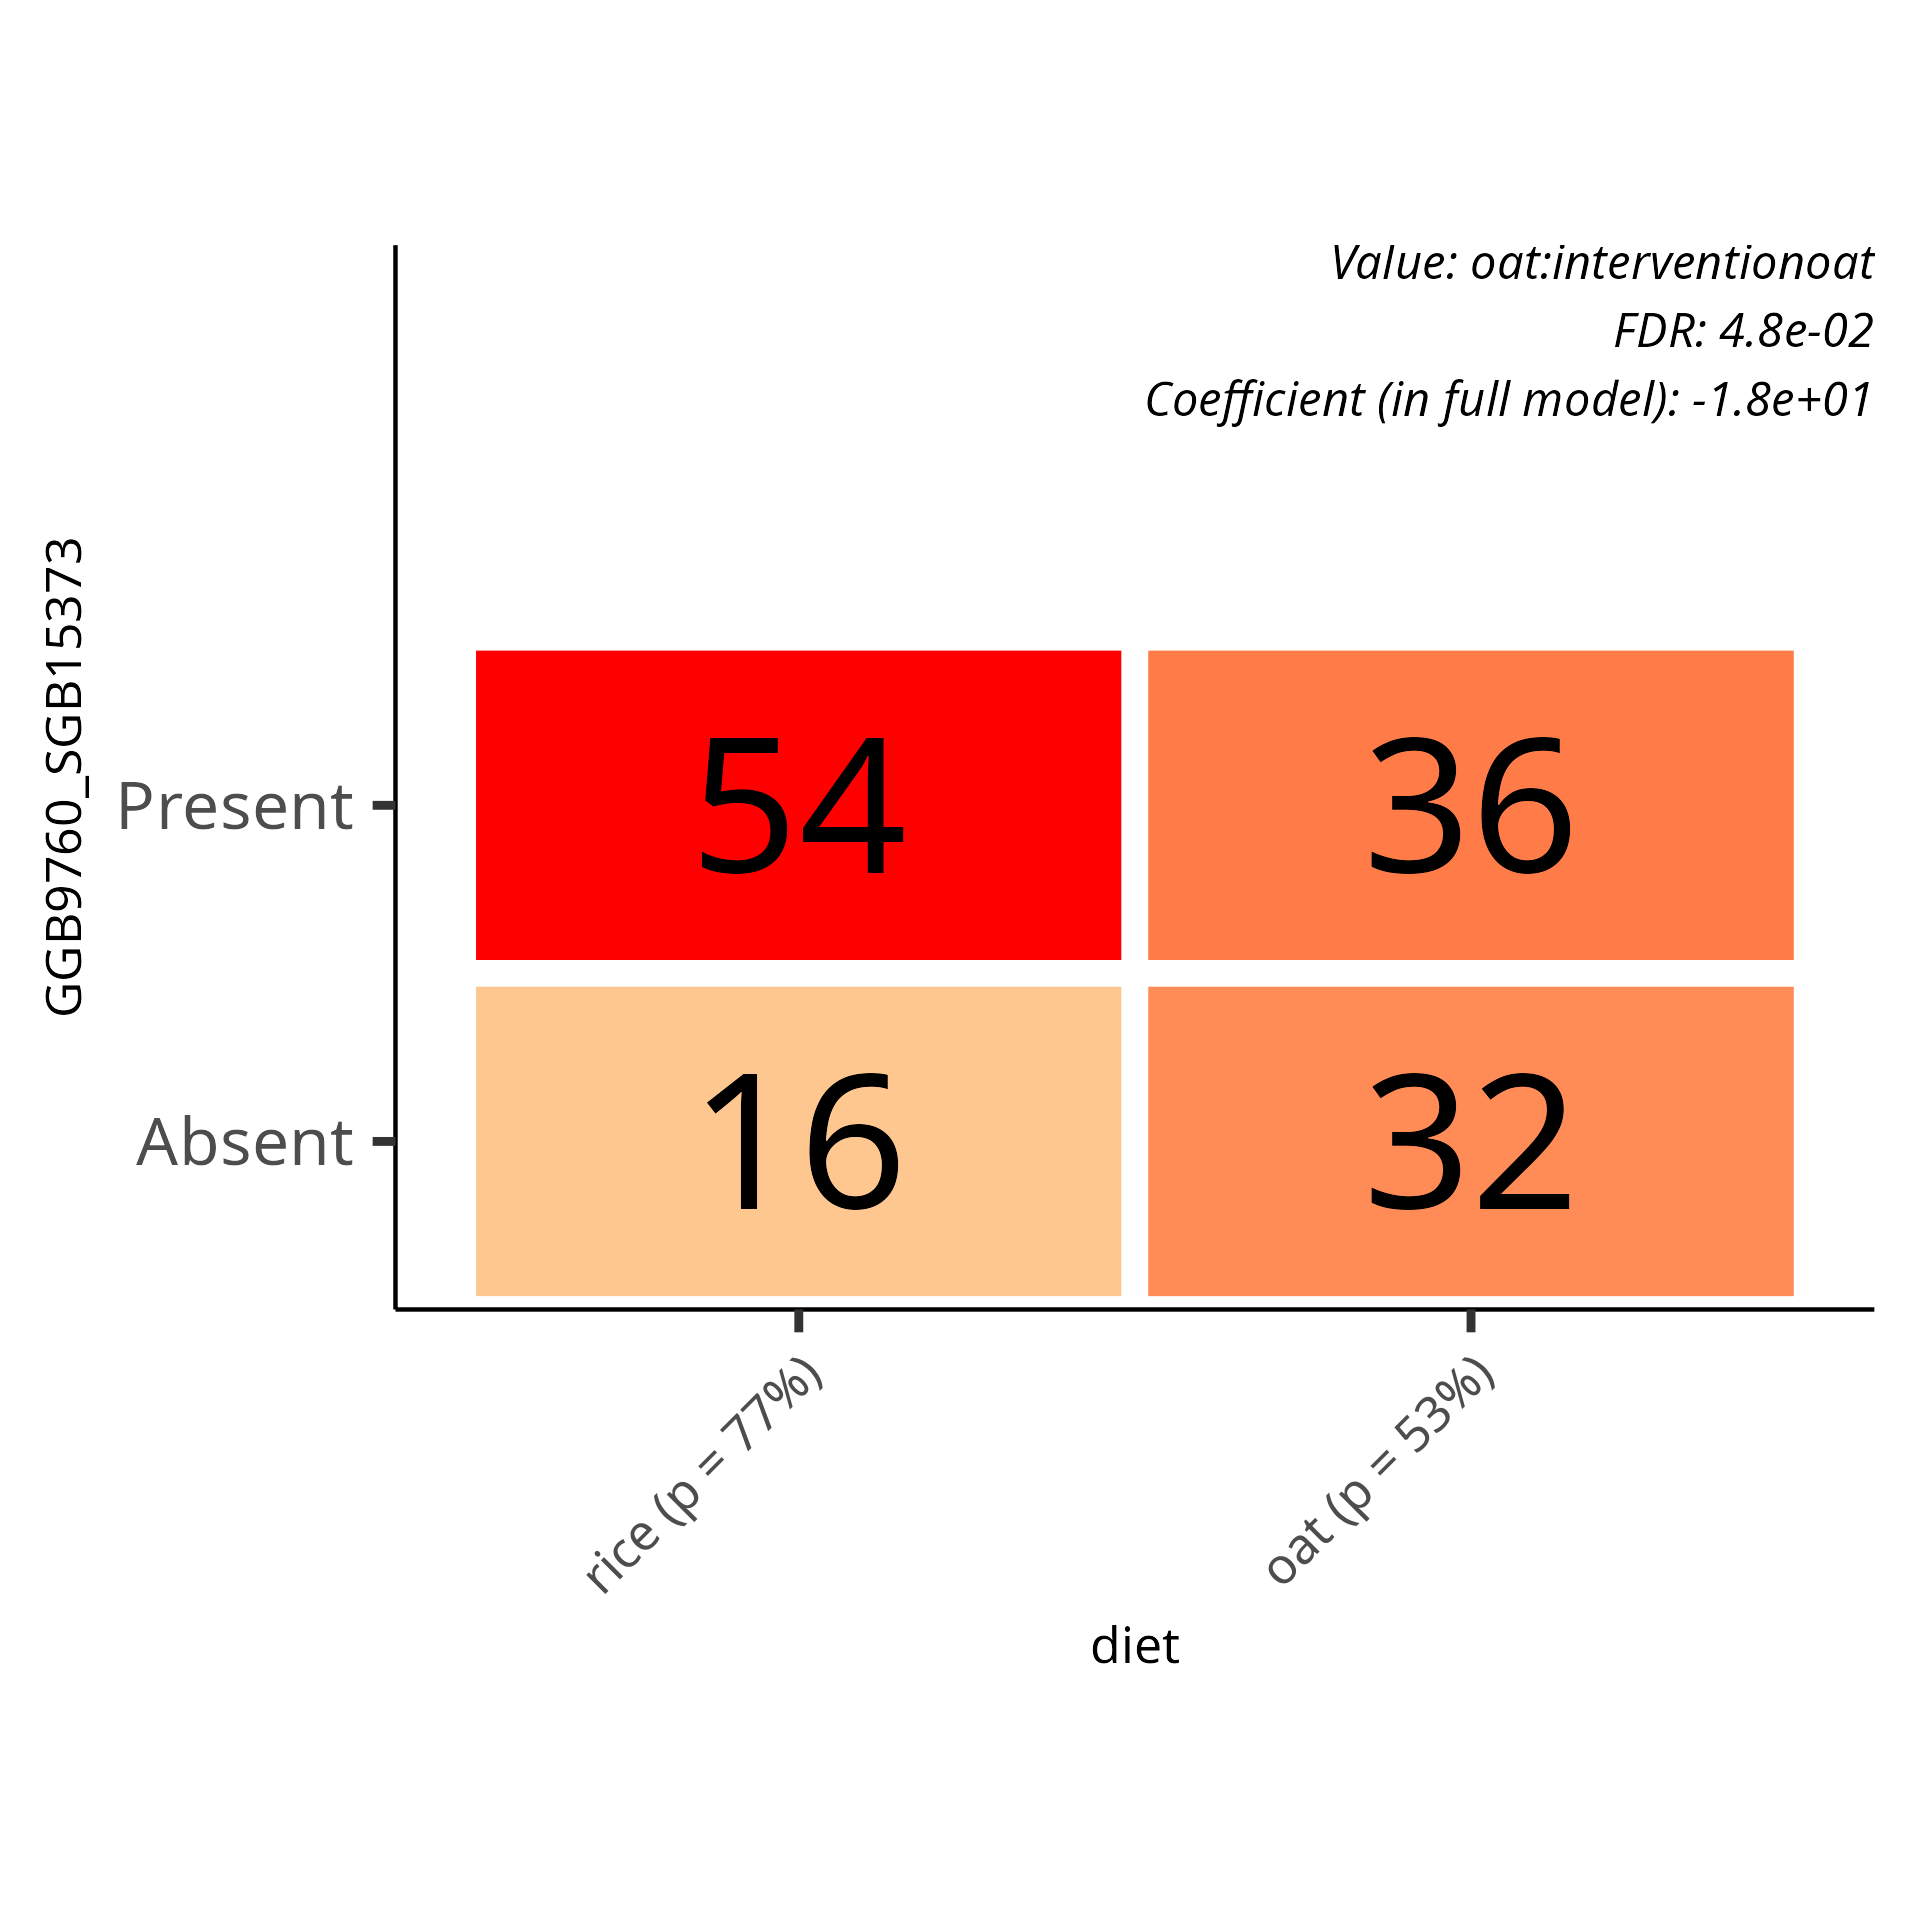
\includegraphics{../../output/daa/daa_taxa/species/figures/association_plots/diet/logistic/diet_GGB9760_SGB15373_logistic.png}\\
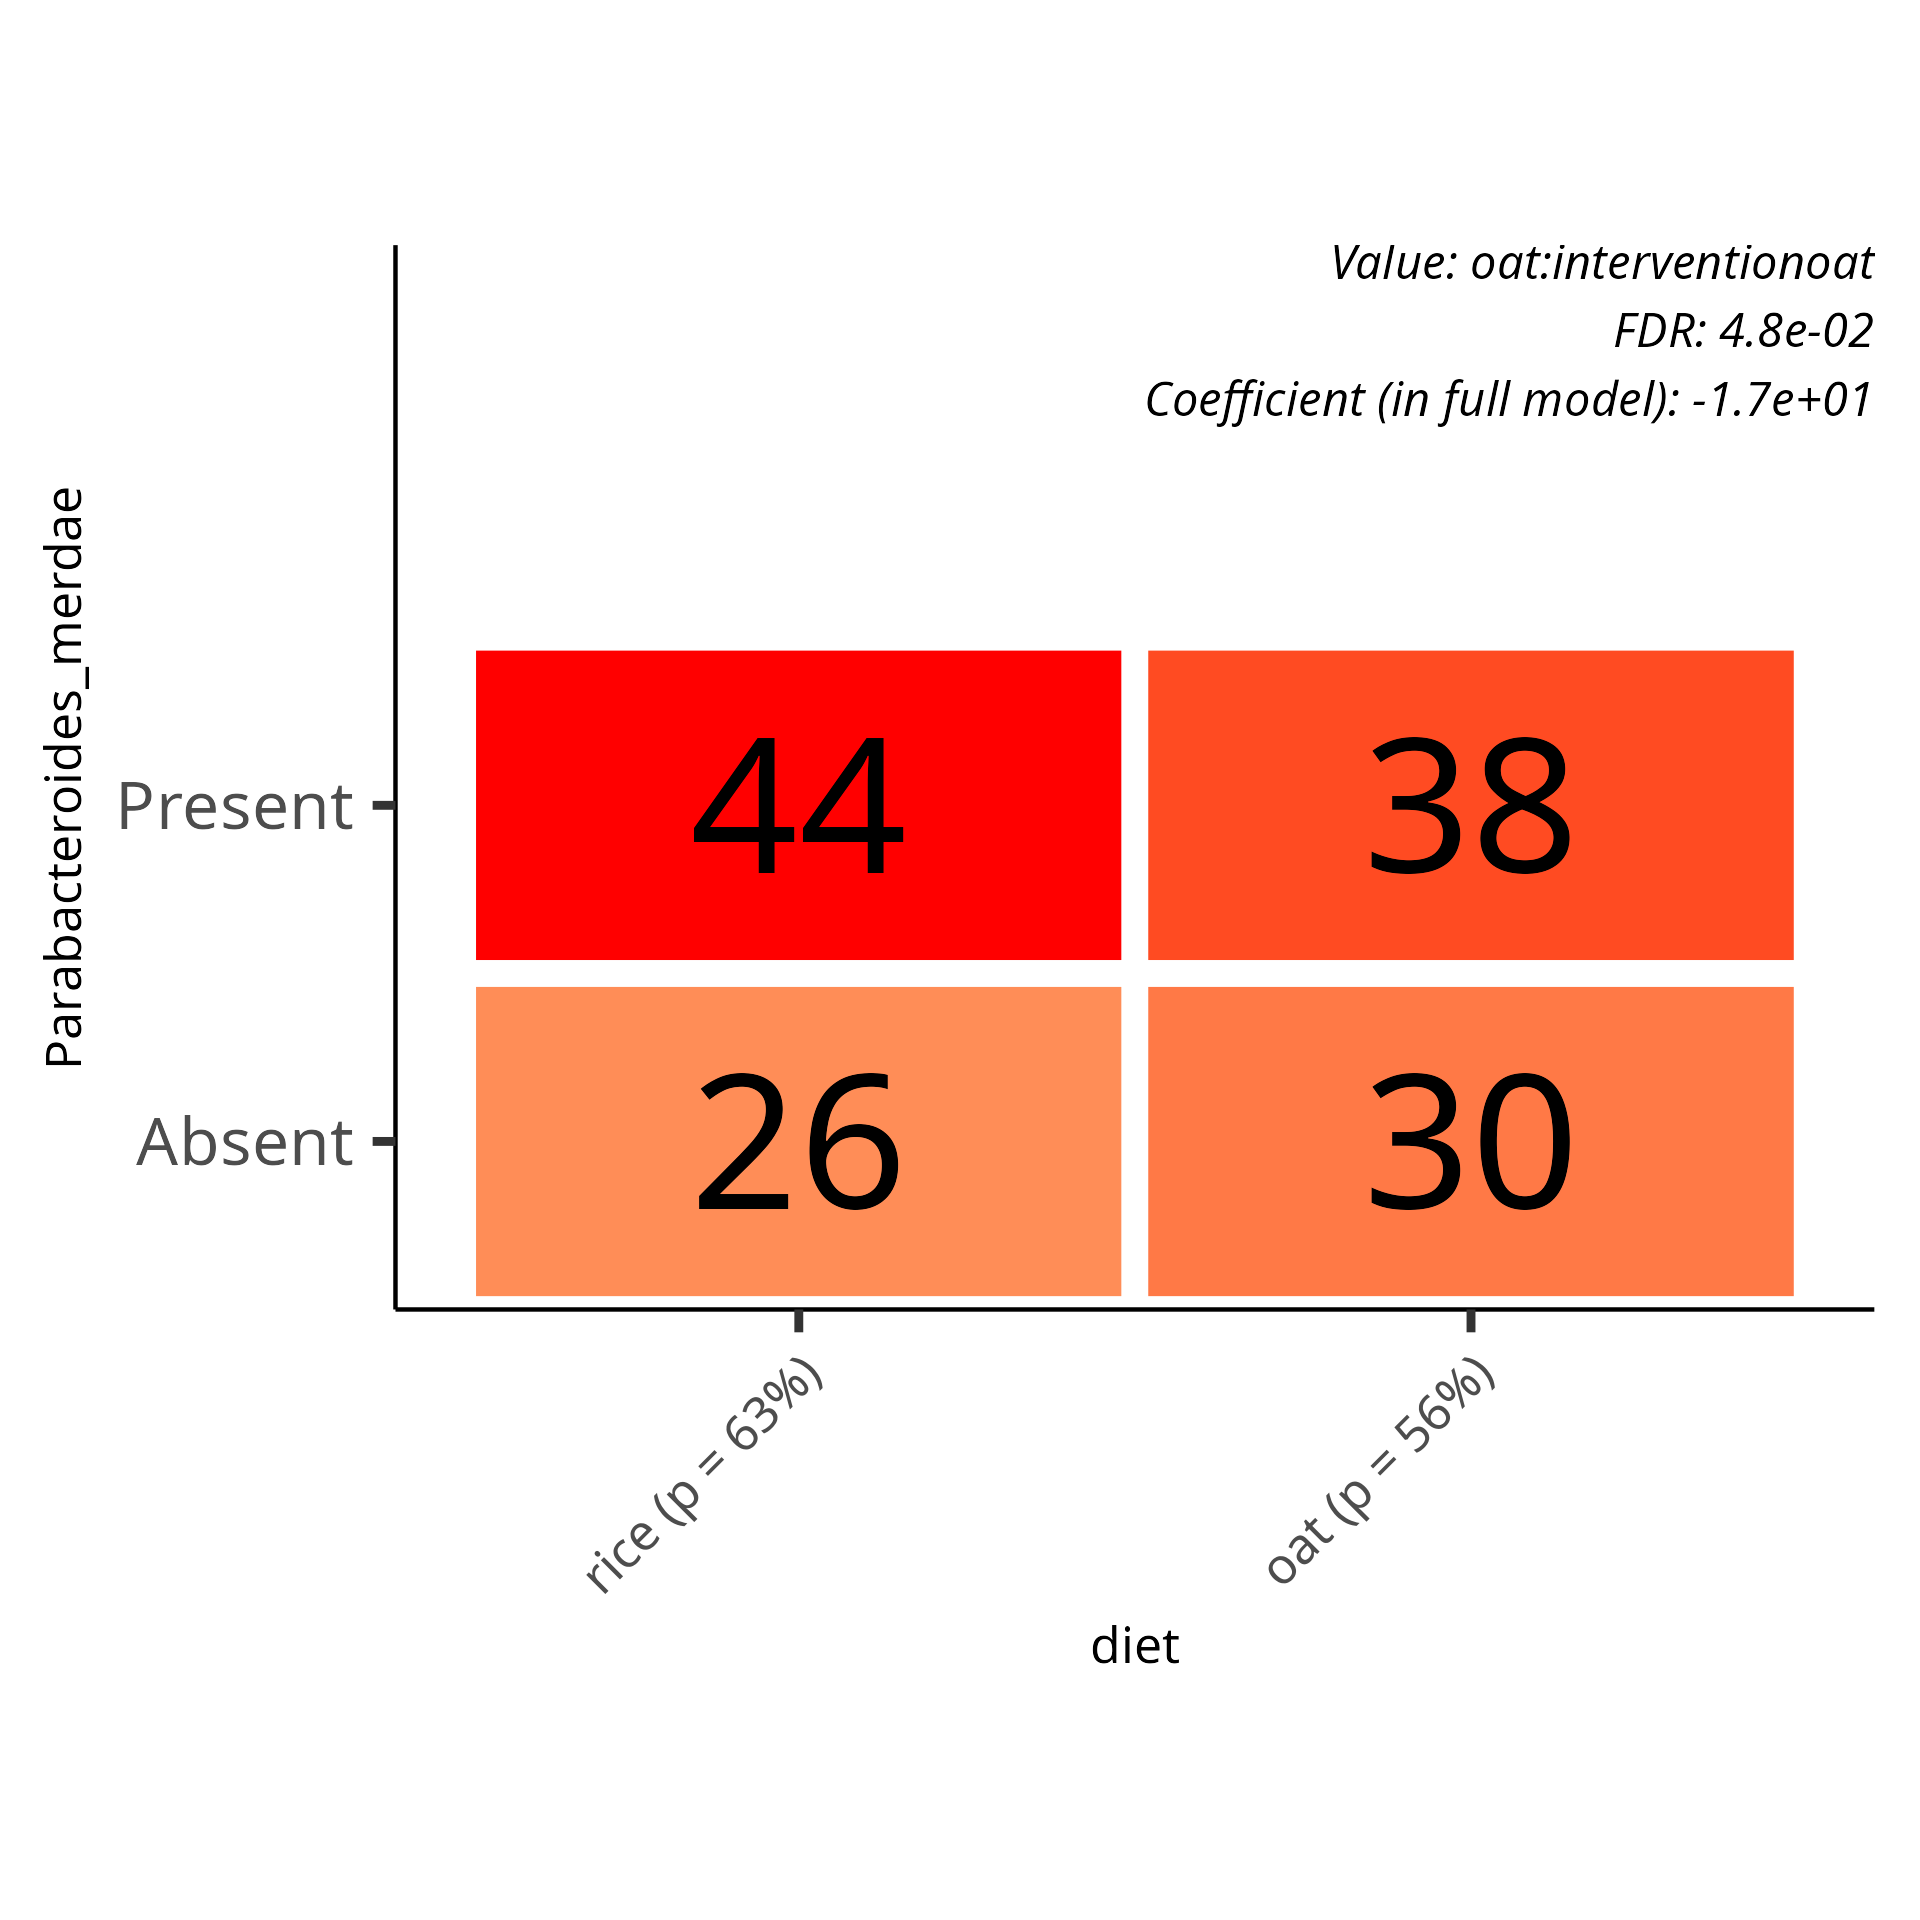
\includegraphics{../../output/daa/daa_taxa/species/figures/association_plots/diet/logistic/diet_Parabacteroides_merdae_logistic.png}\\
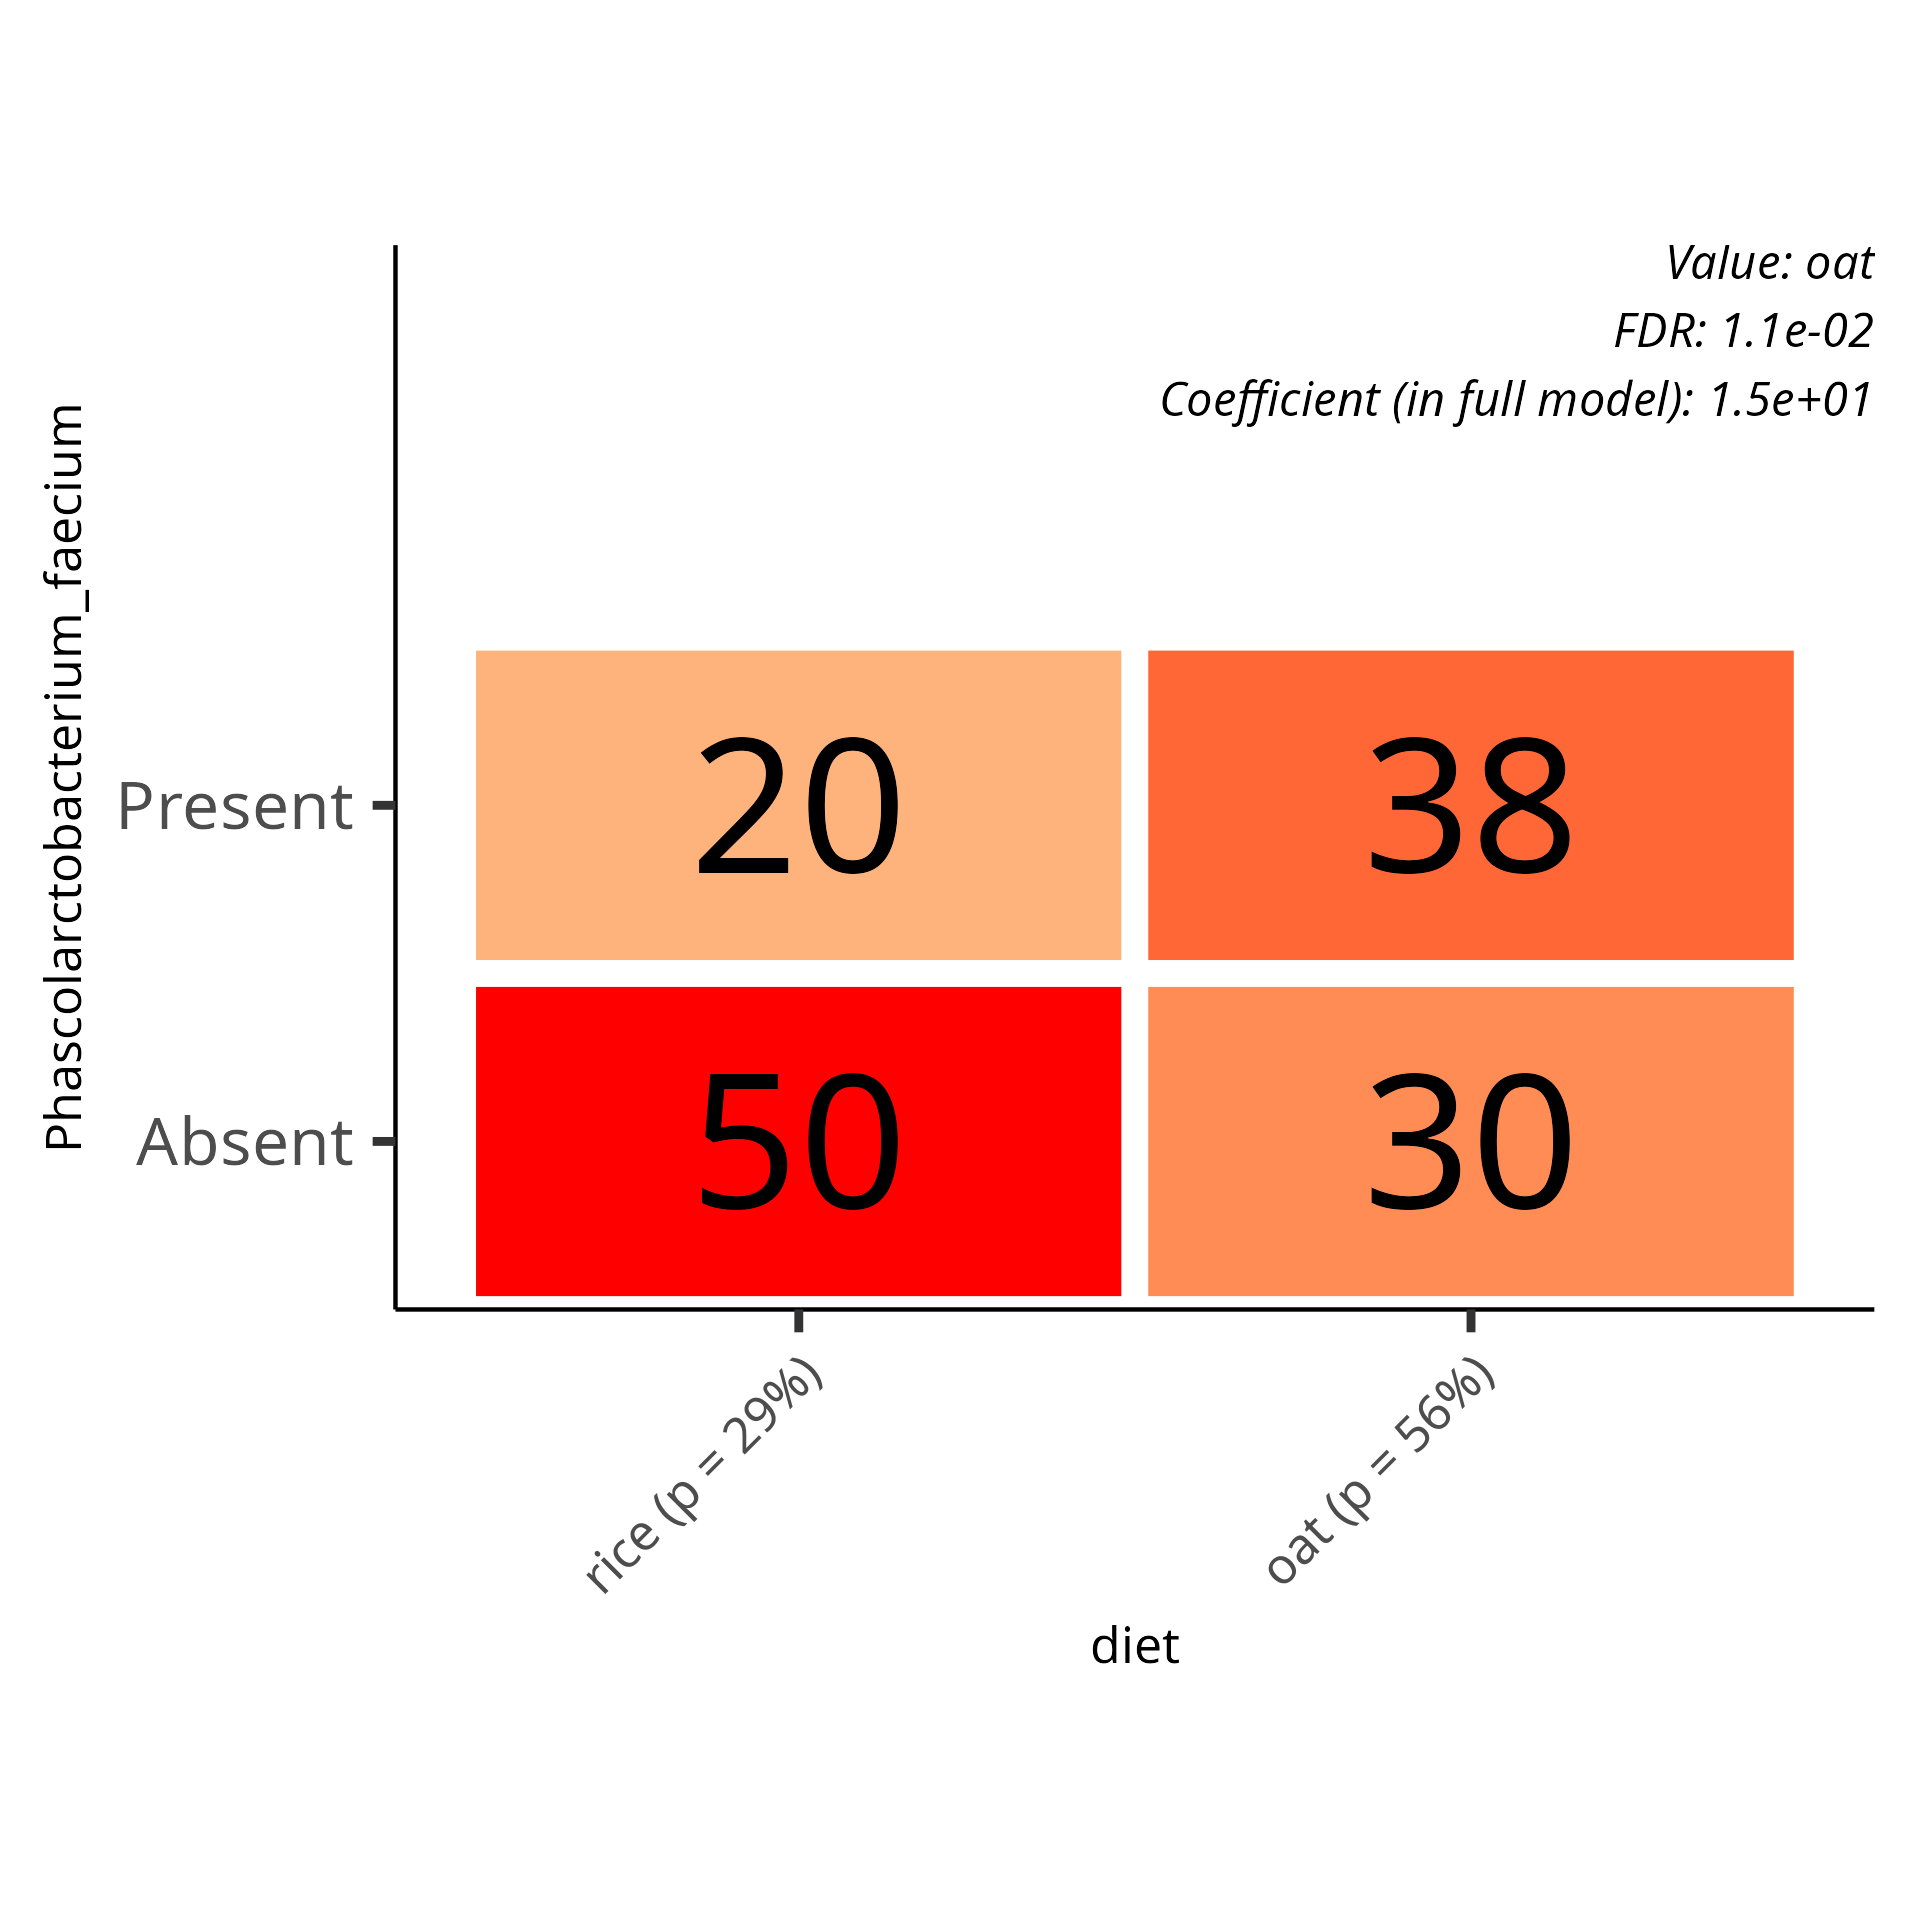
\includegraphics{../../output/daa/daa_taxa/species/figures/association_plots/diet/logistic/diet_Phascolarctobacterium_faecium_logistic.png}
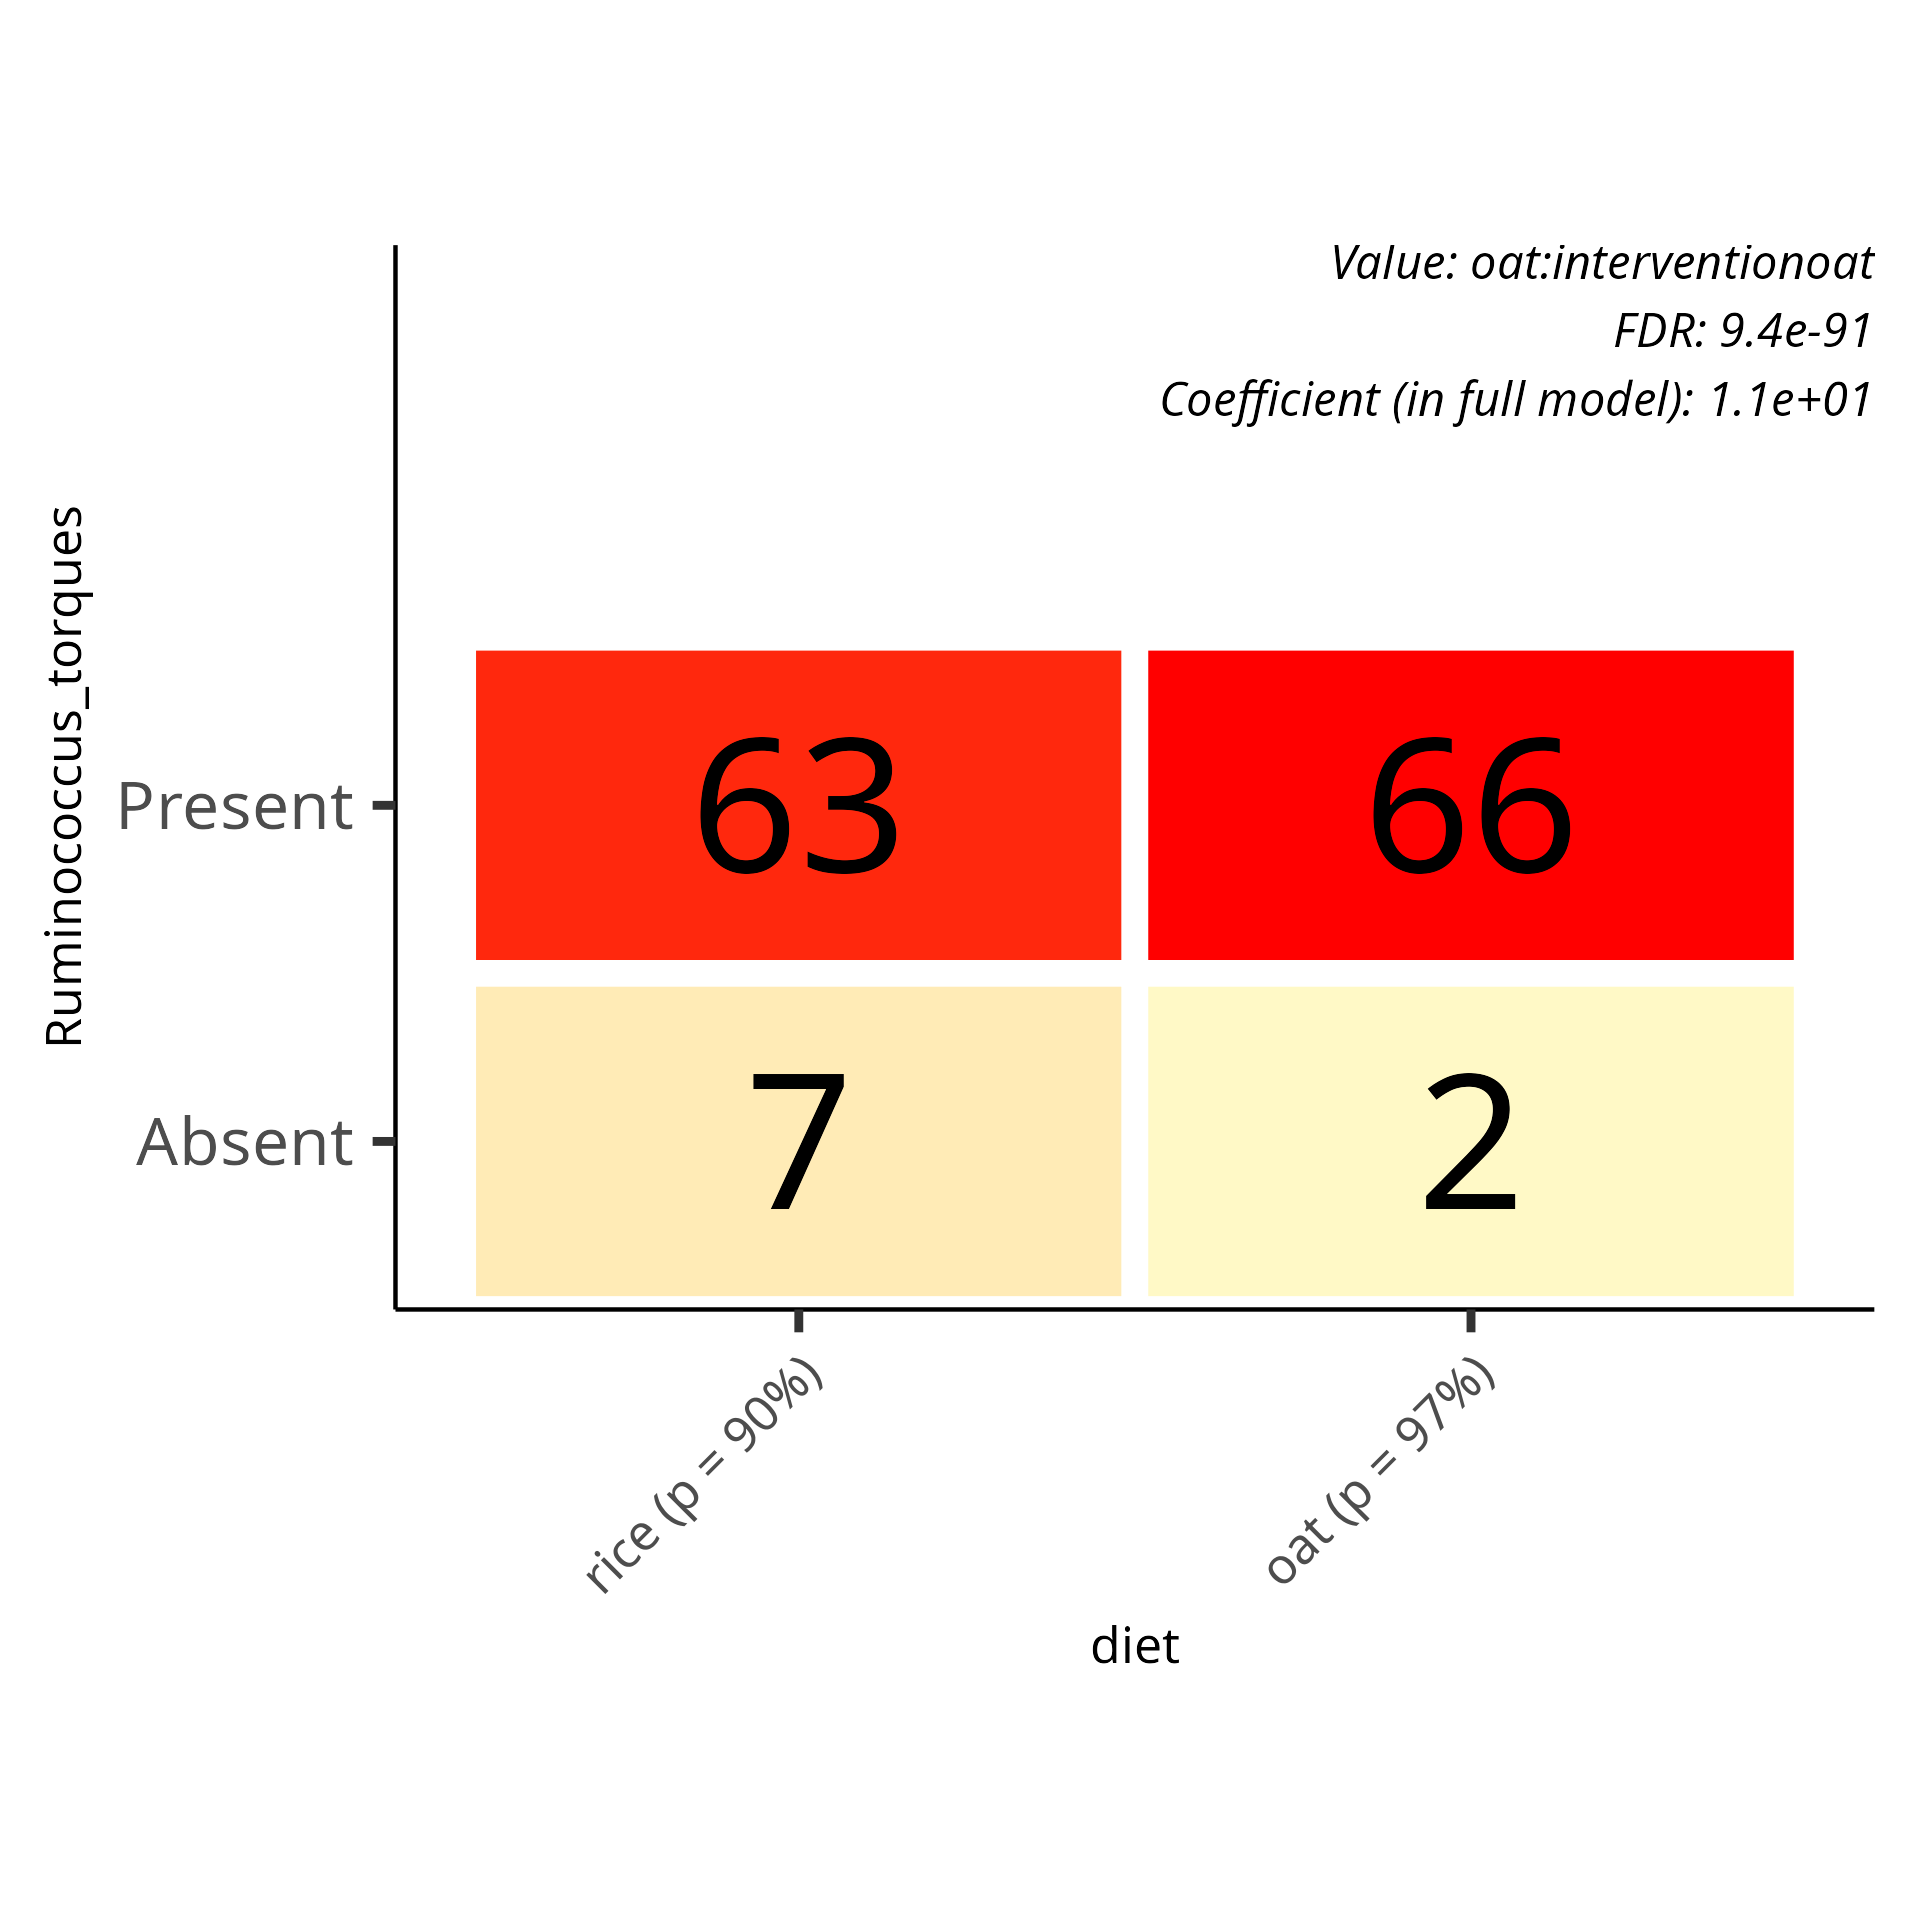
\includegraphics{../../output/daa/daa_taxa/species/figures/association_plots/diet/logistic/diet_Ruminococcus_torques_logistic.png}\\
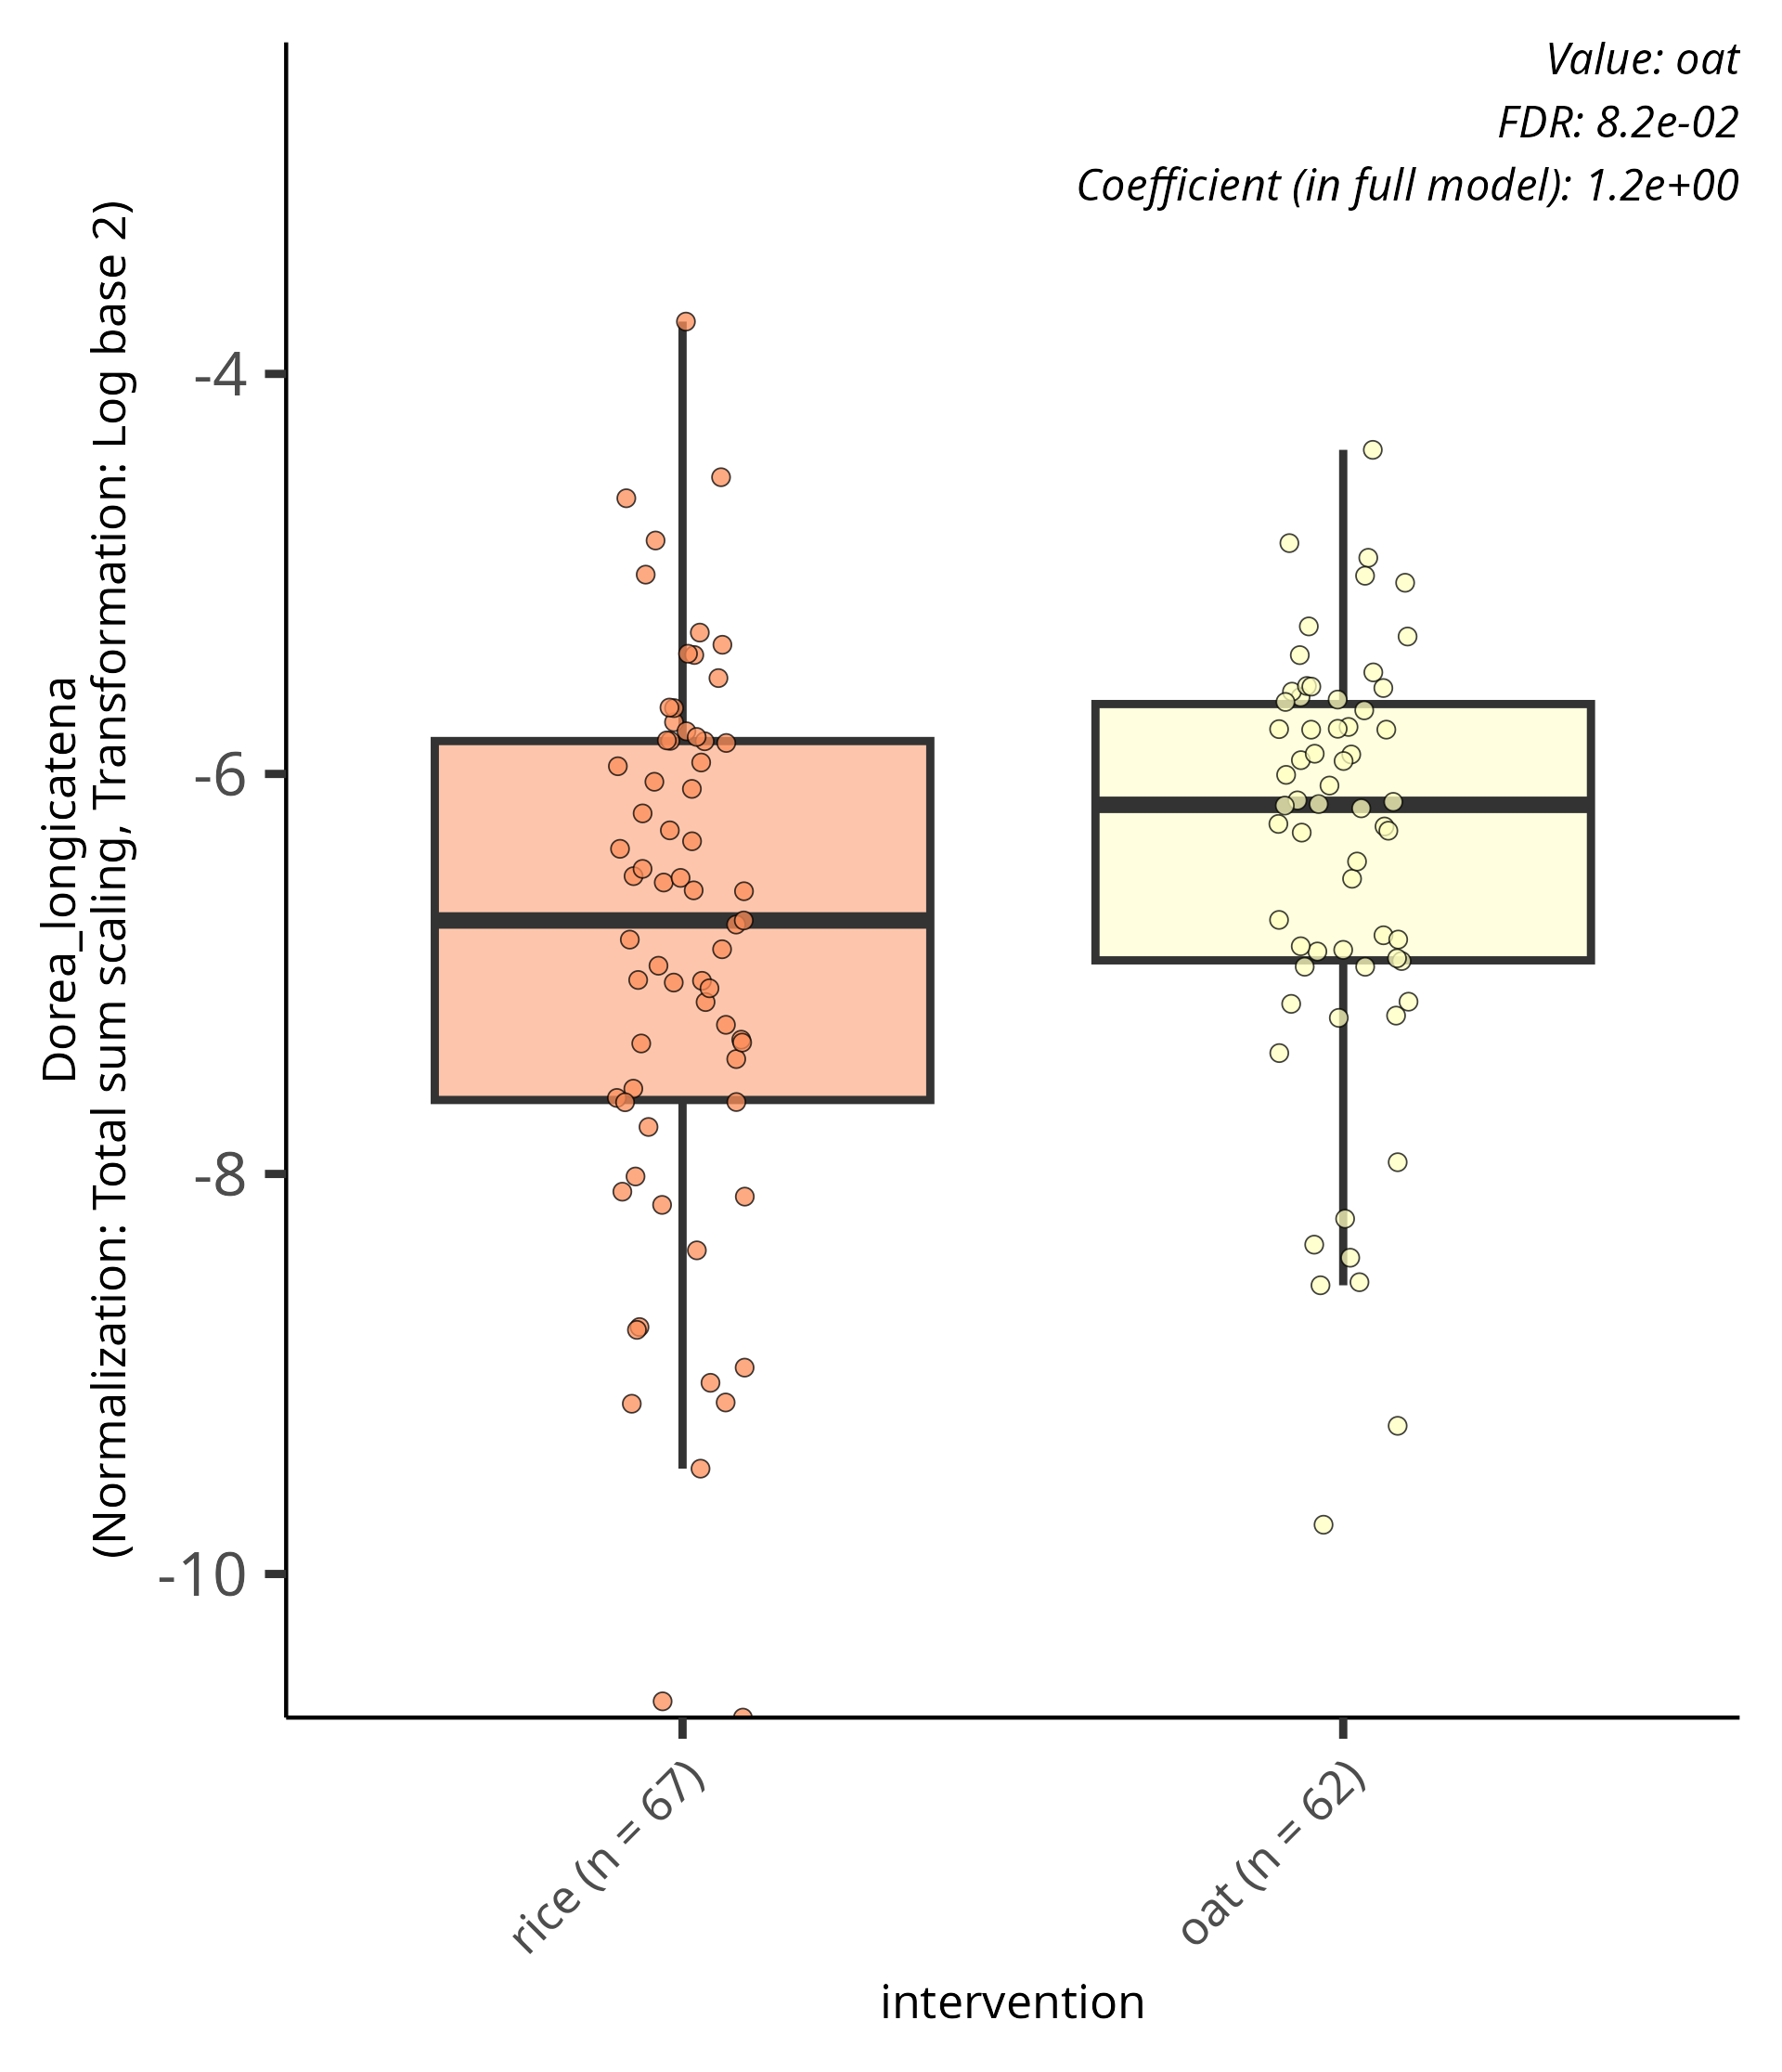
\includegraphics{../../output/daa/daa_taxa/species/figures/association_plots/intervention/linear/intervention_Dorea_longicatena_linear.png}\\
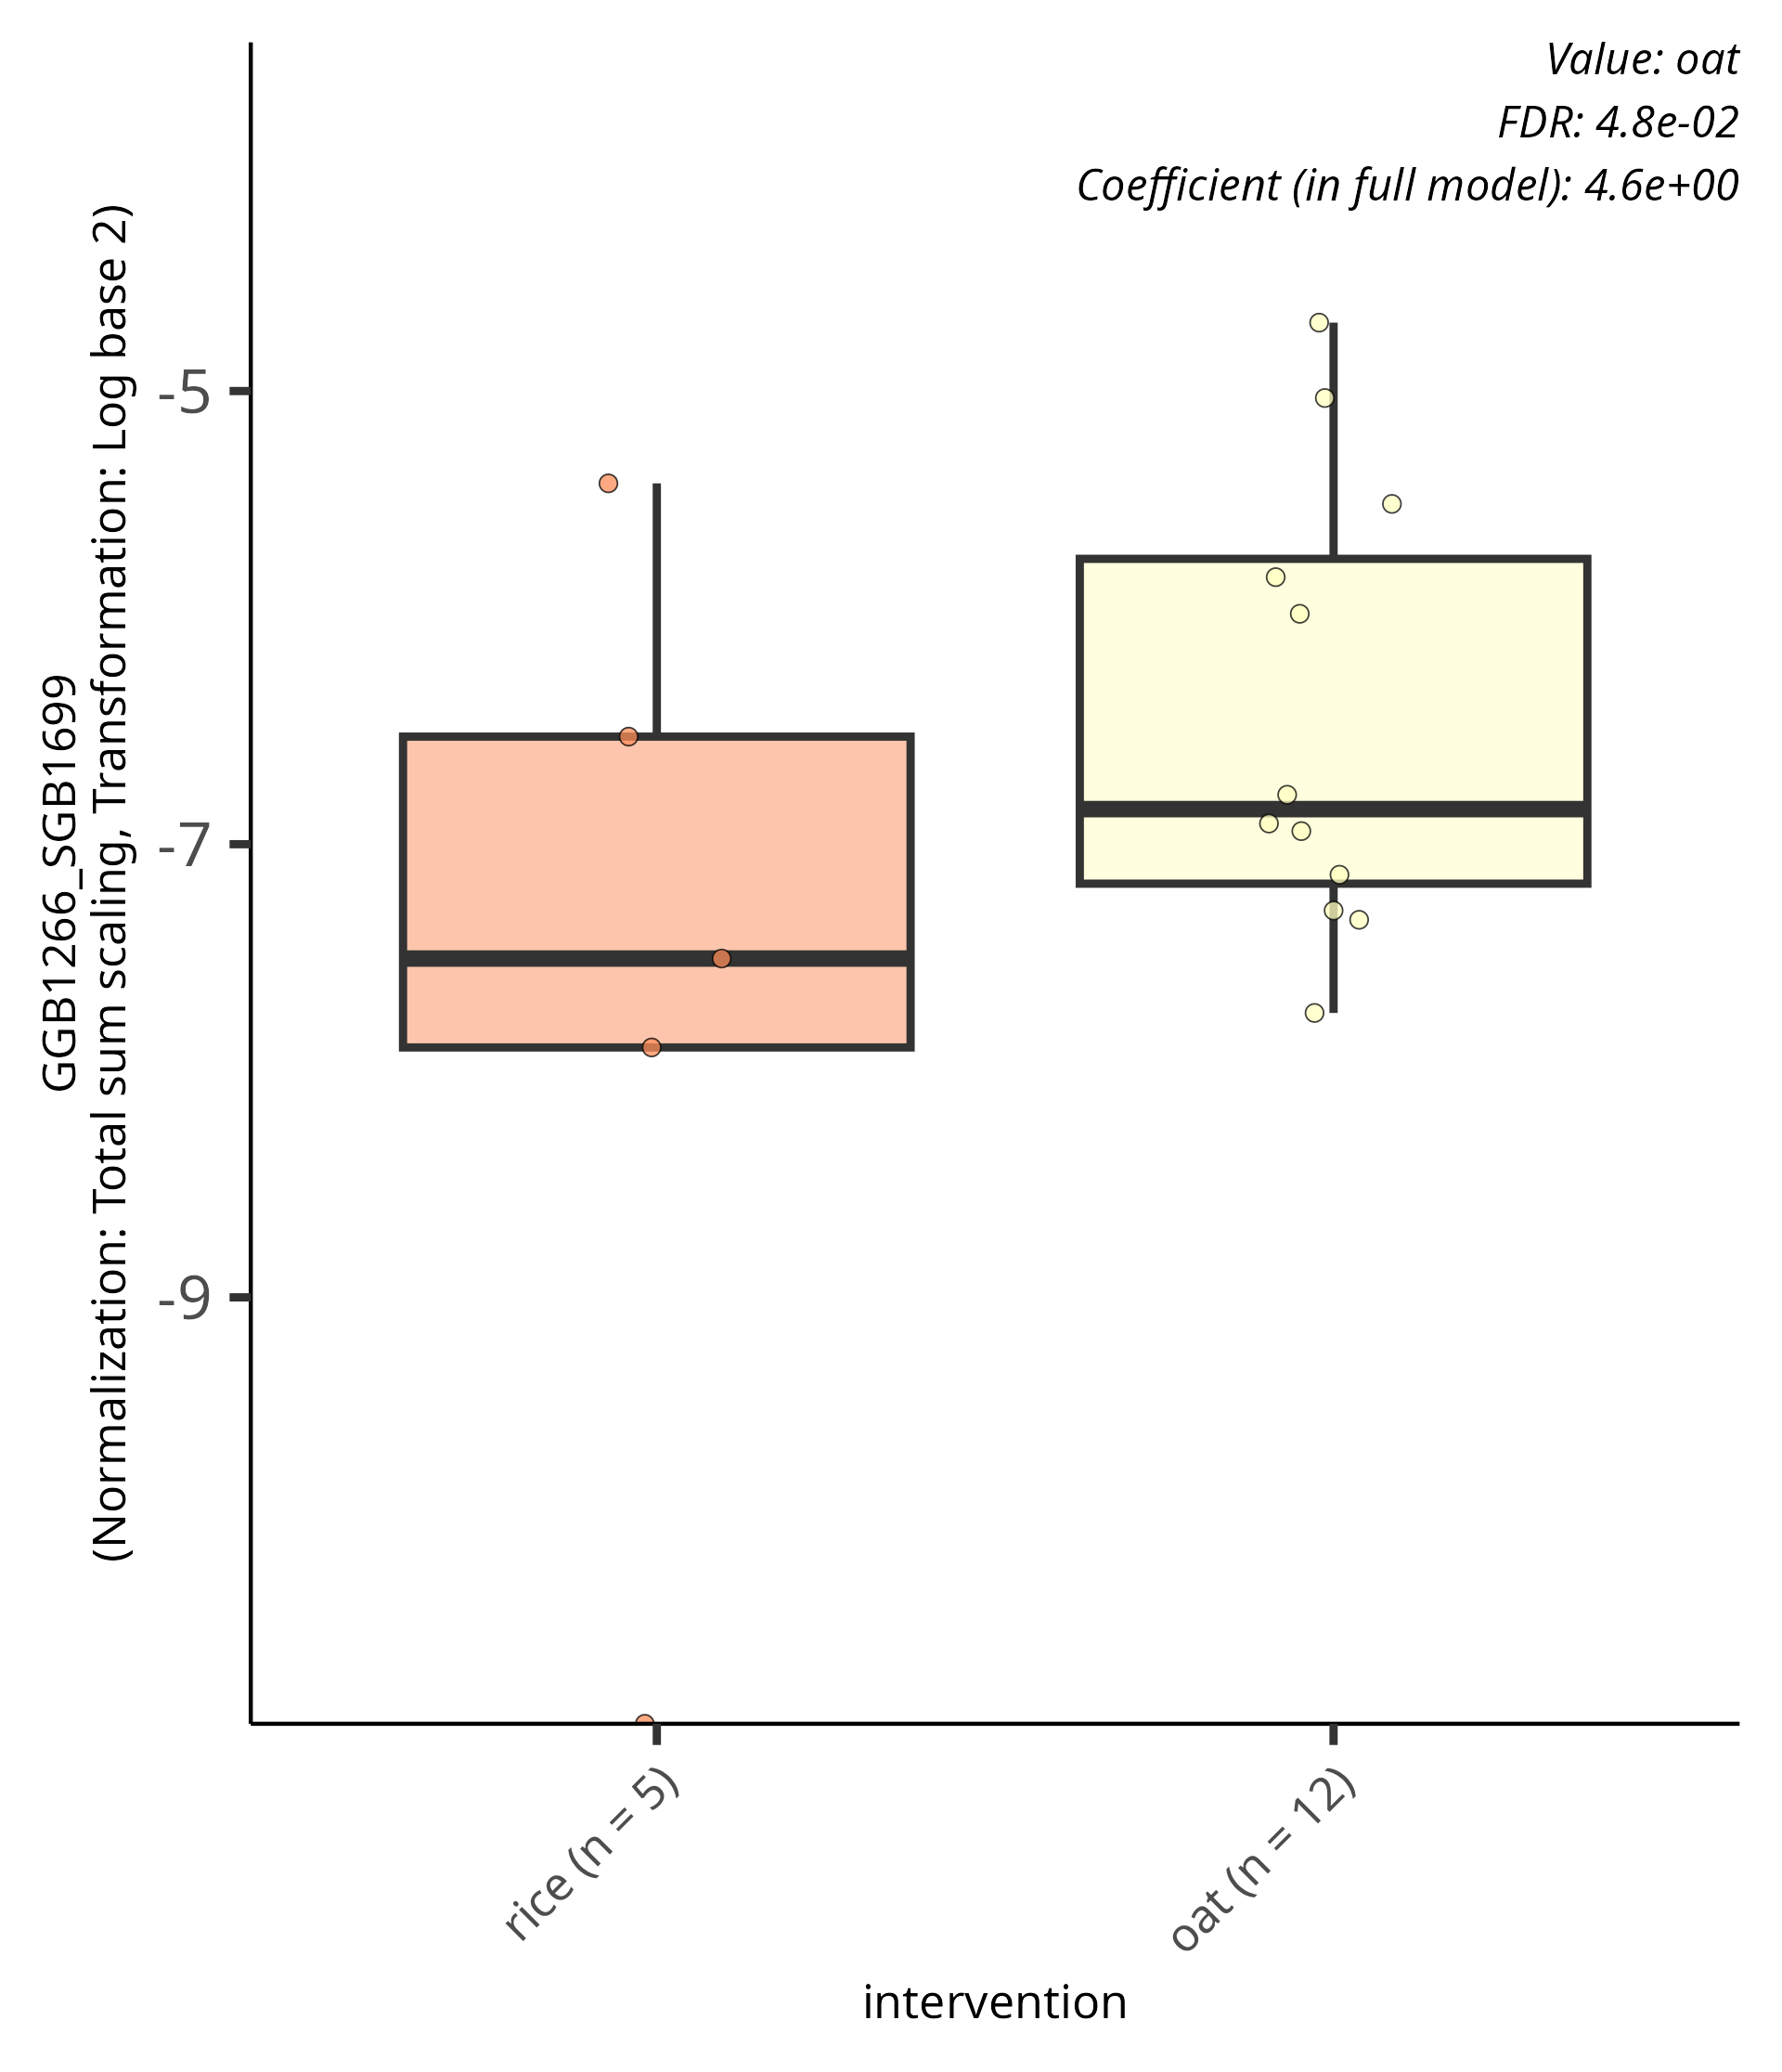
\includegraphics{../../output/daa/daa_taxa/species/figures/association_plots/intervention/linear/intervention_GGB1266_SGB1699_linear.png}\\
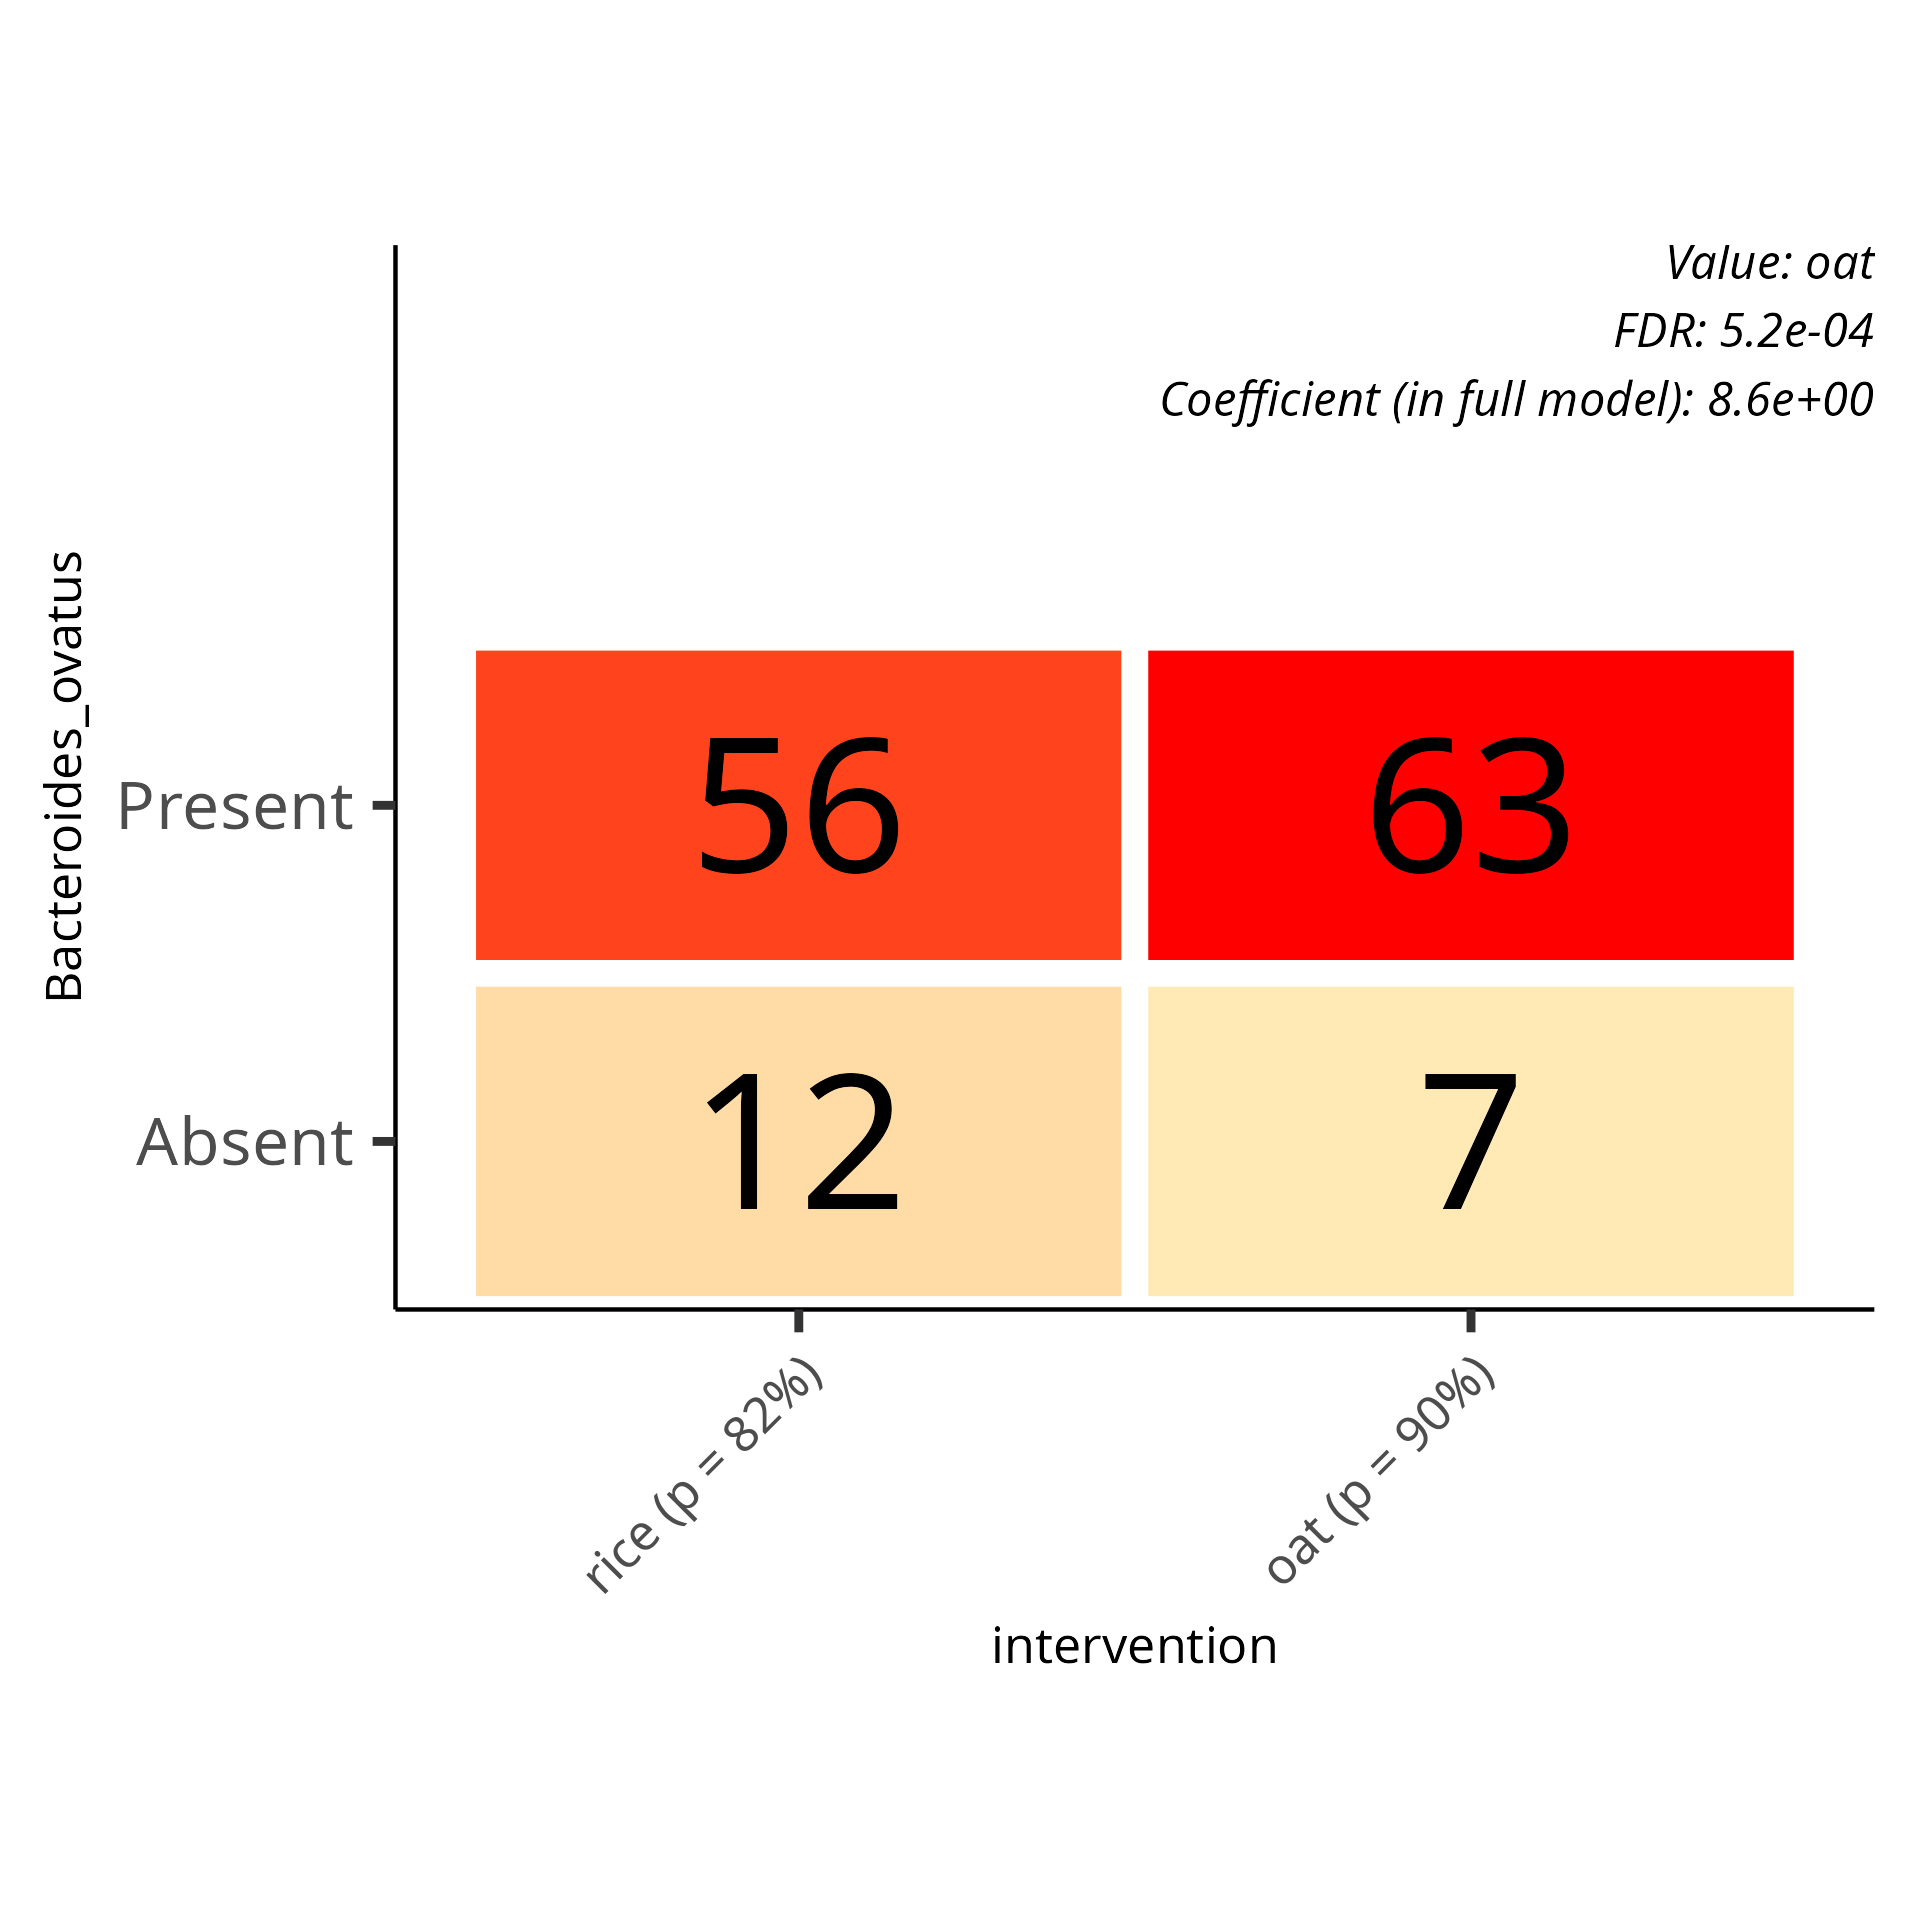
\includegraphics{../../output/daa/daa_taxa/species/figures/association_plots/intervention/logistic/intervention_Bacteroides_ovatus_logistic.png}\\
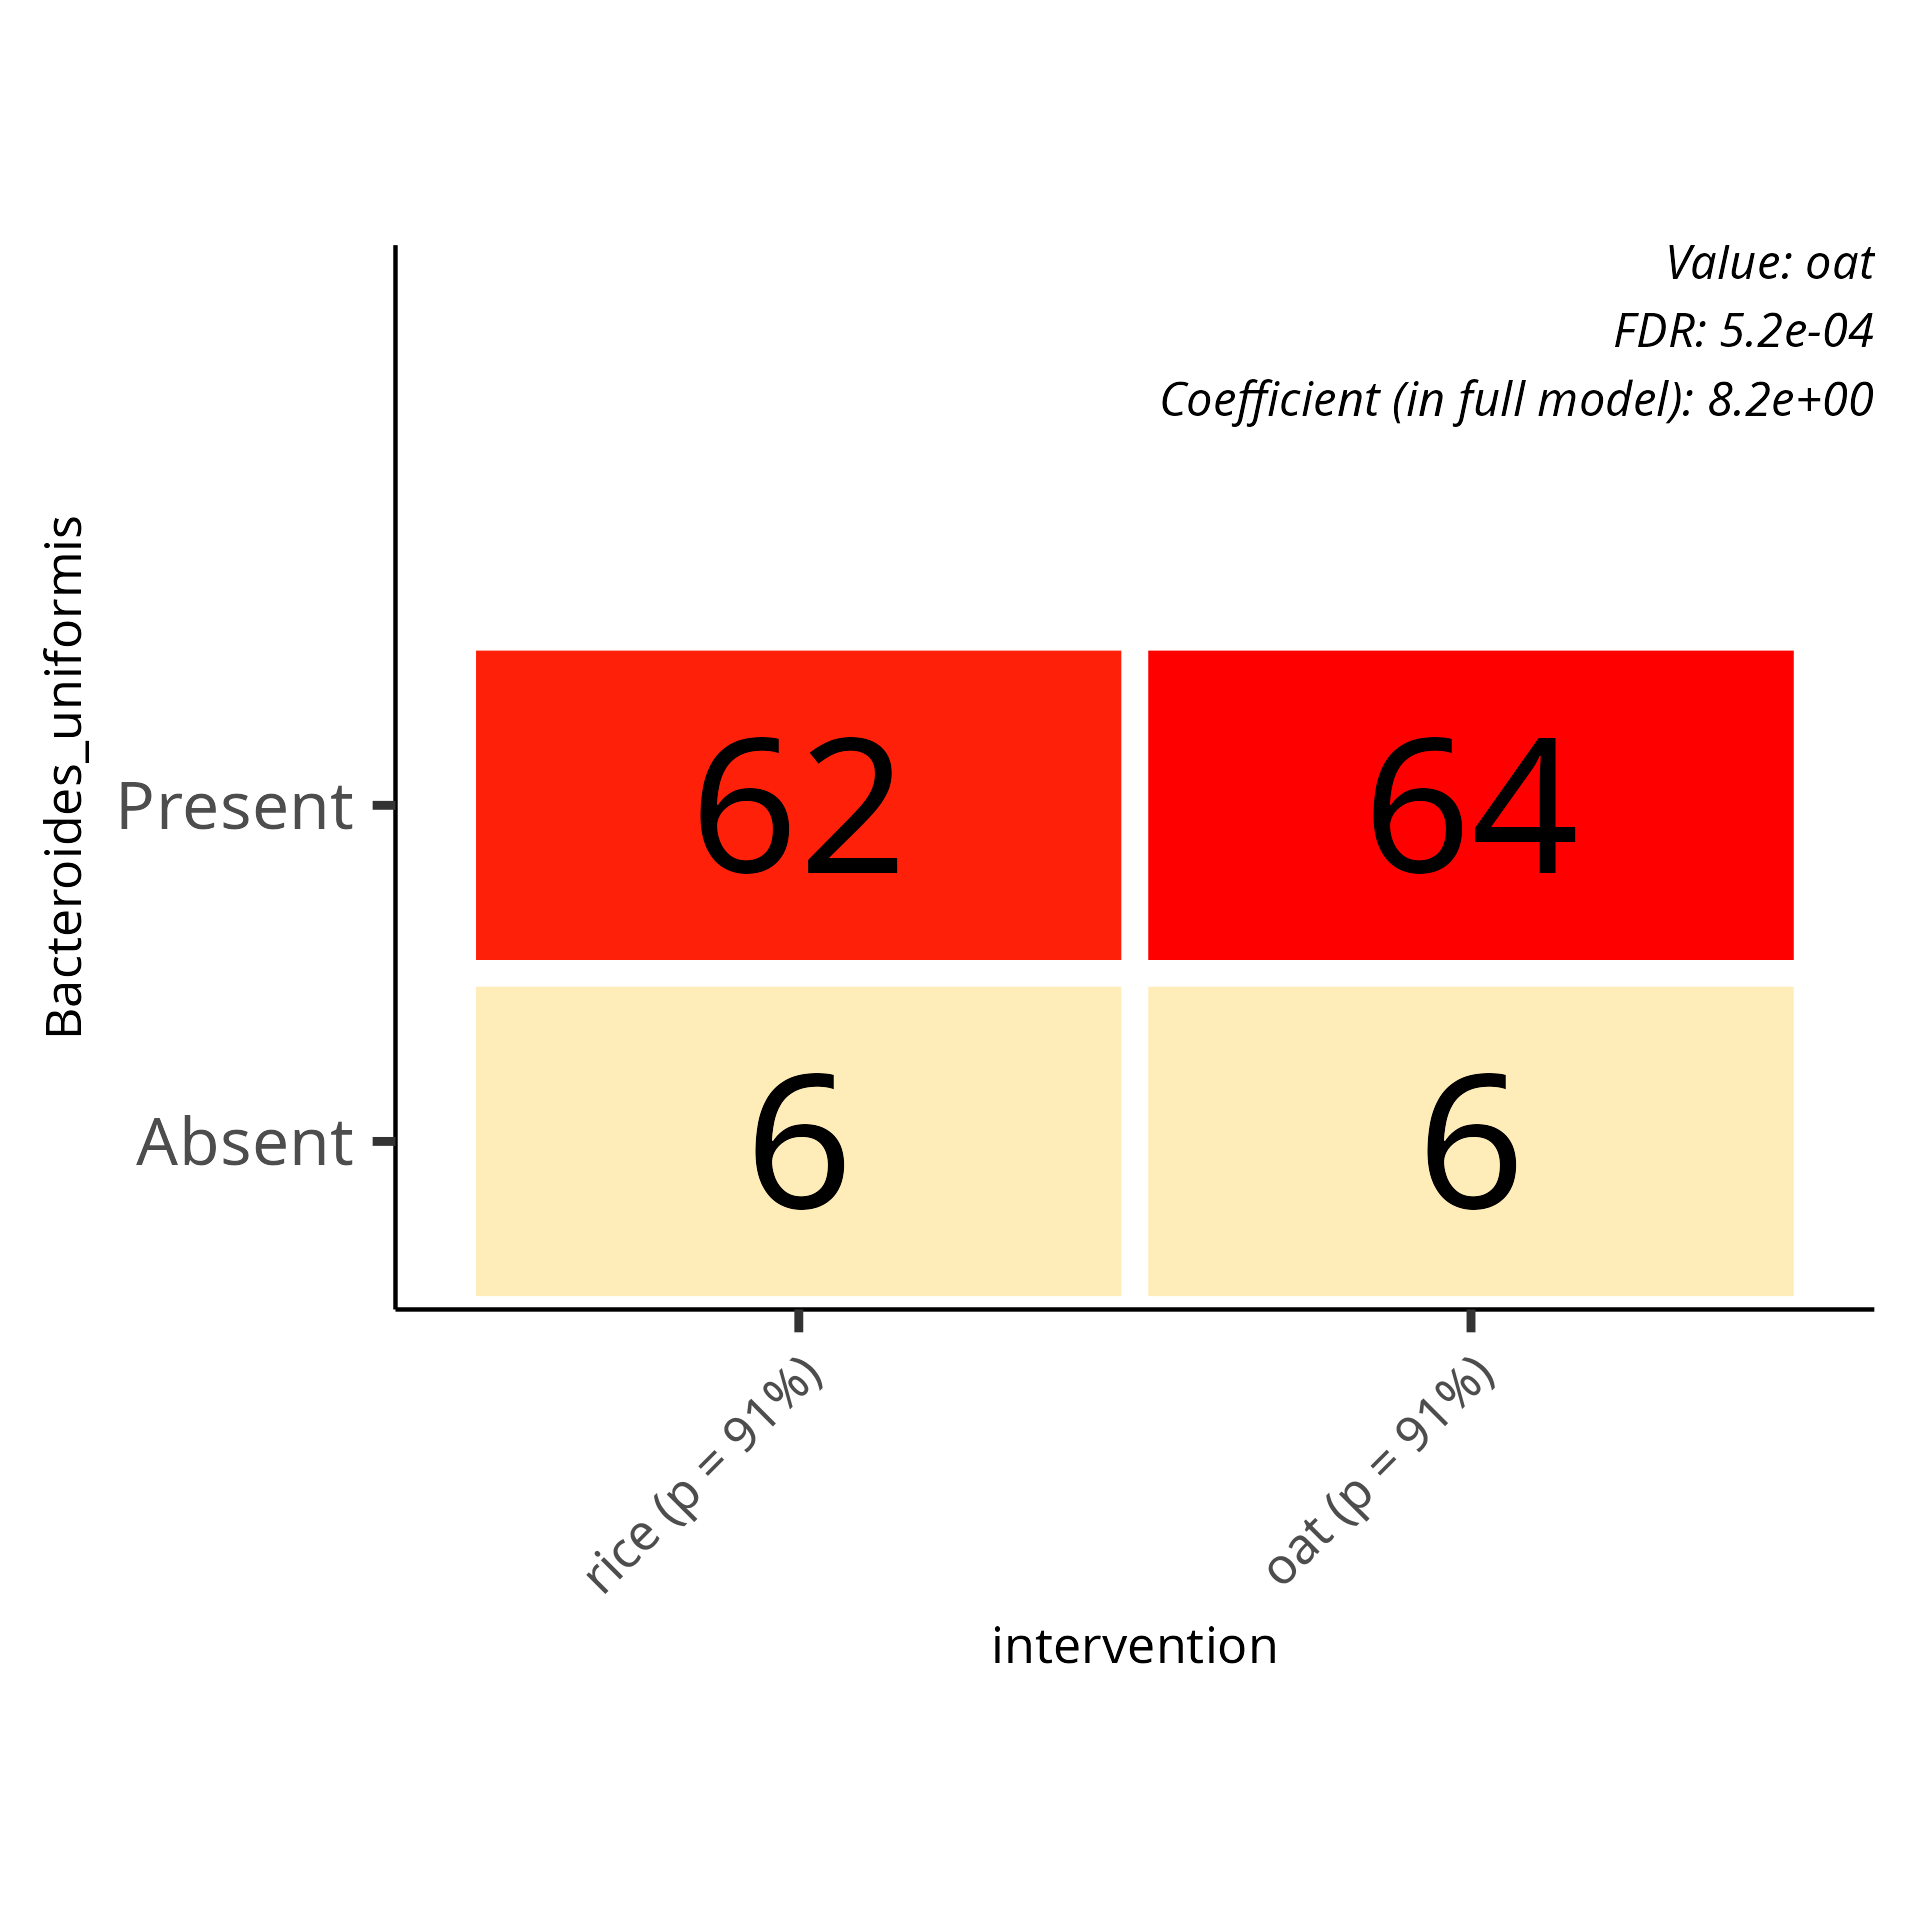
\includegraphics{../../output/daa/daa_taxa/species/figures/association_plots/intervention/logistic/intervention_Bacteroides_uniformis_logistic.png}\\
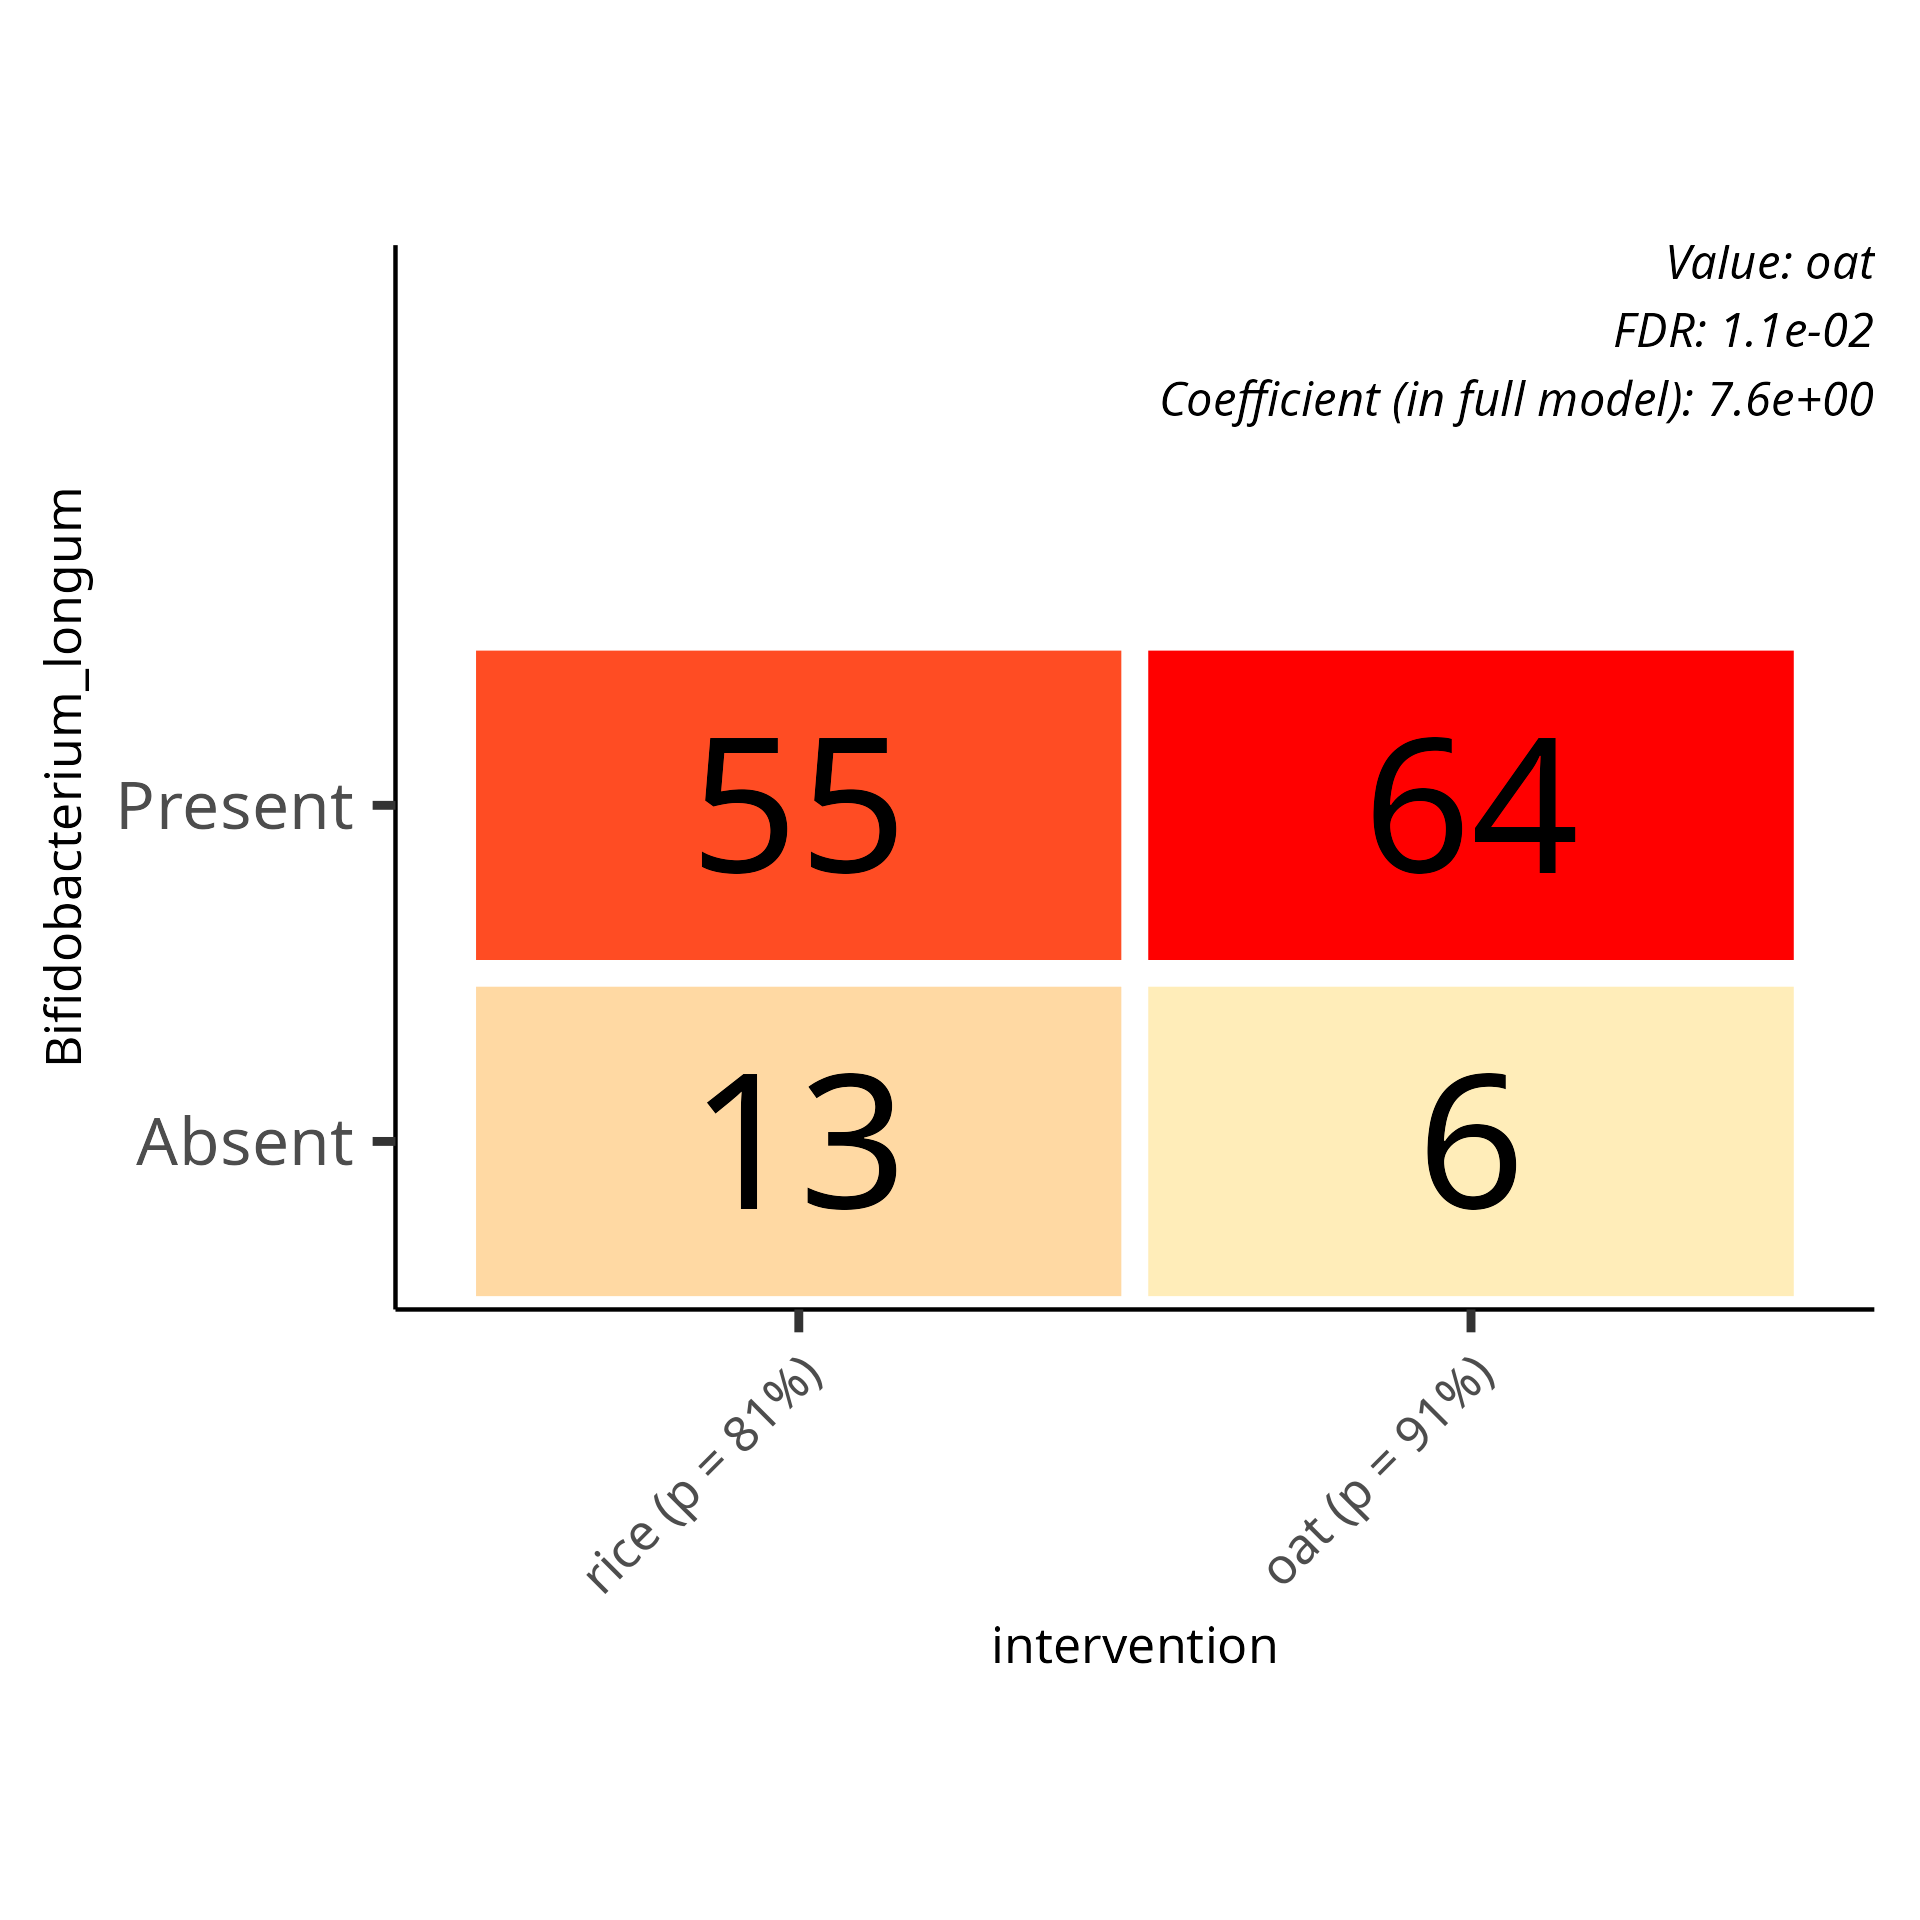
\includegraphics{../../output/daa/daa_taxa/species/figures/association_plots/intervention/logistic/intervention_Bifidobacterium_longum_logistic.png}\\
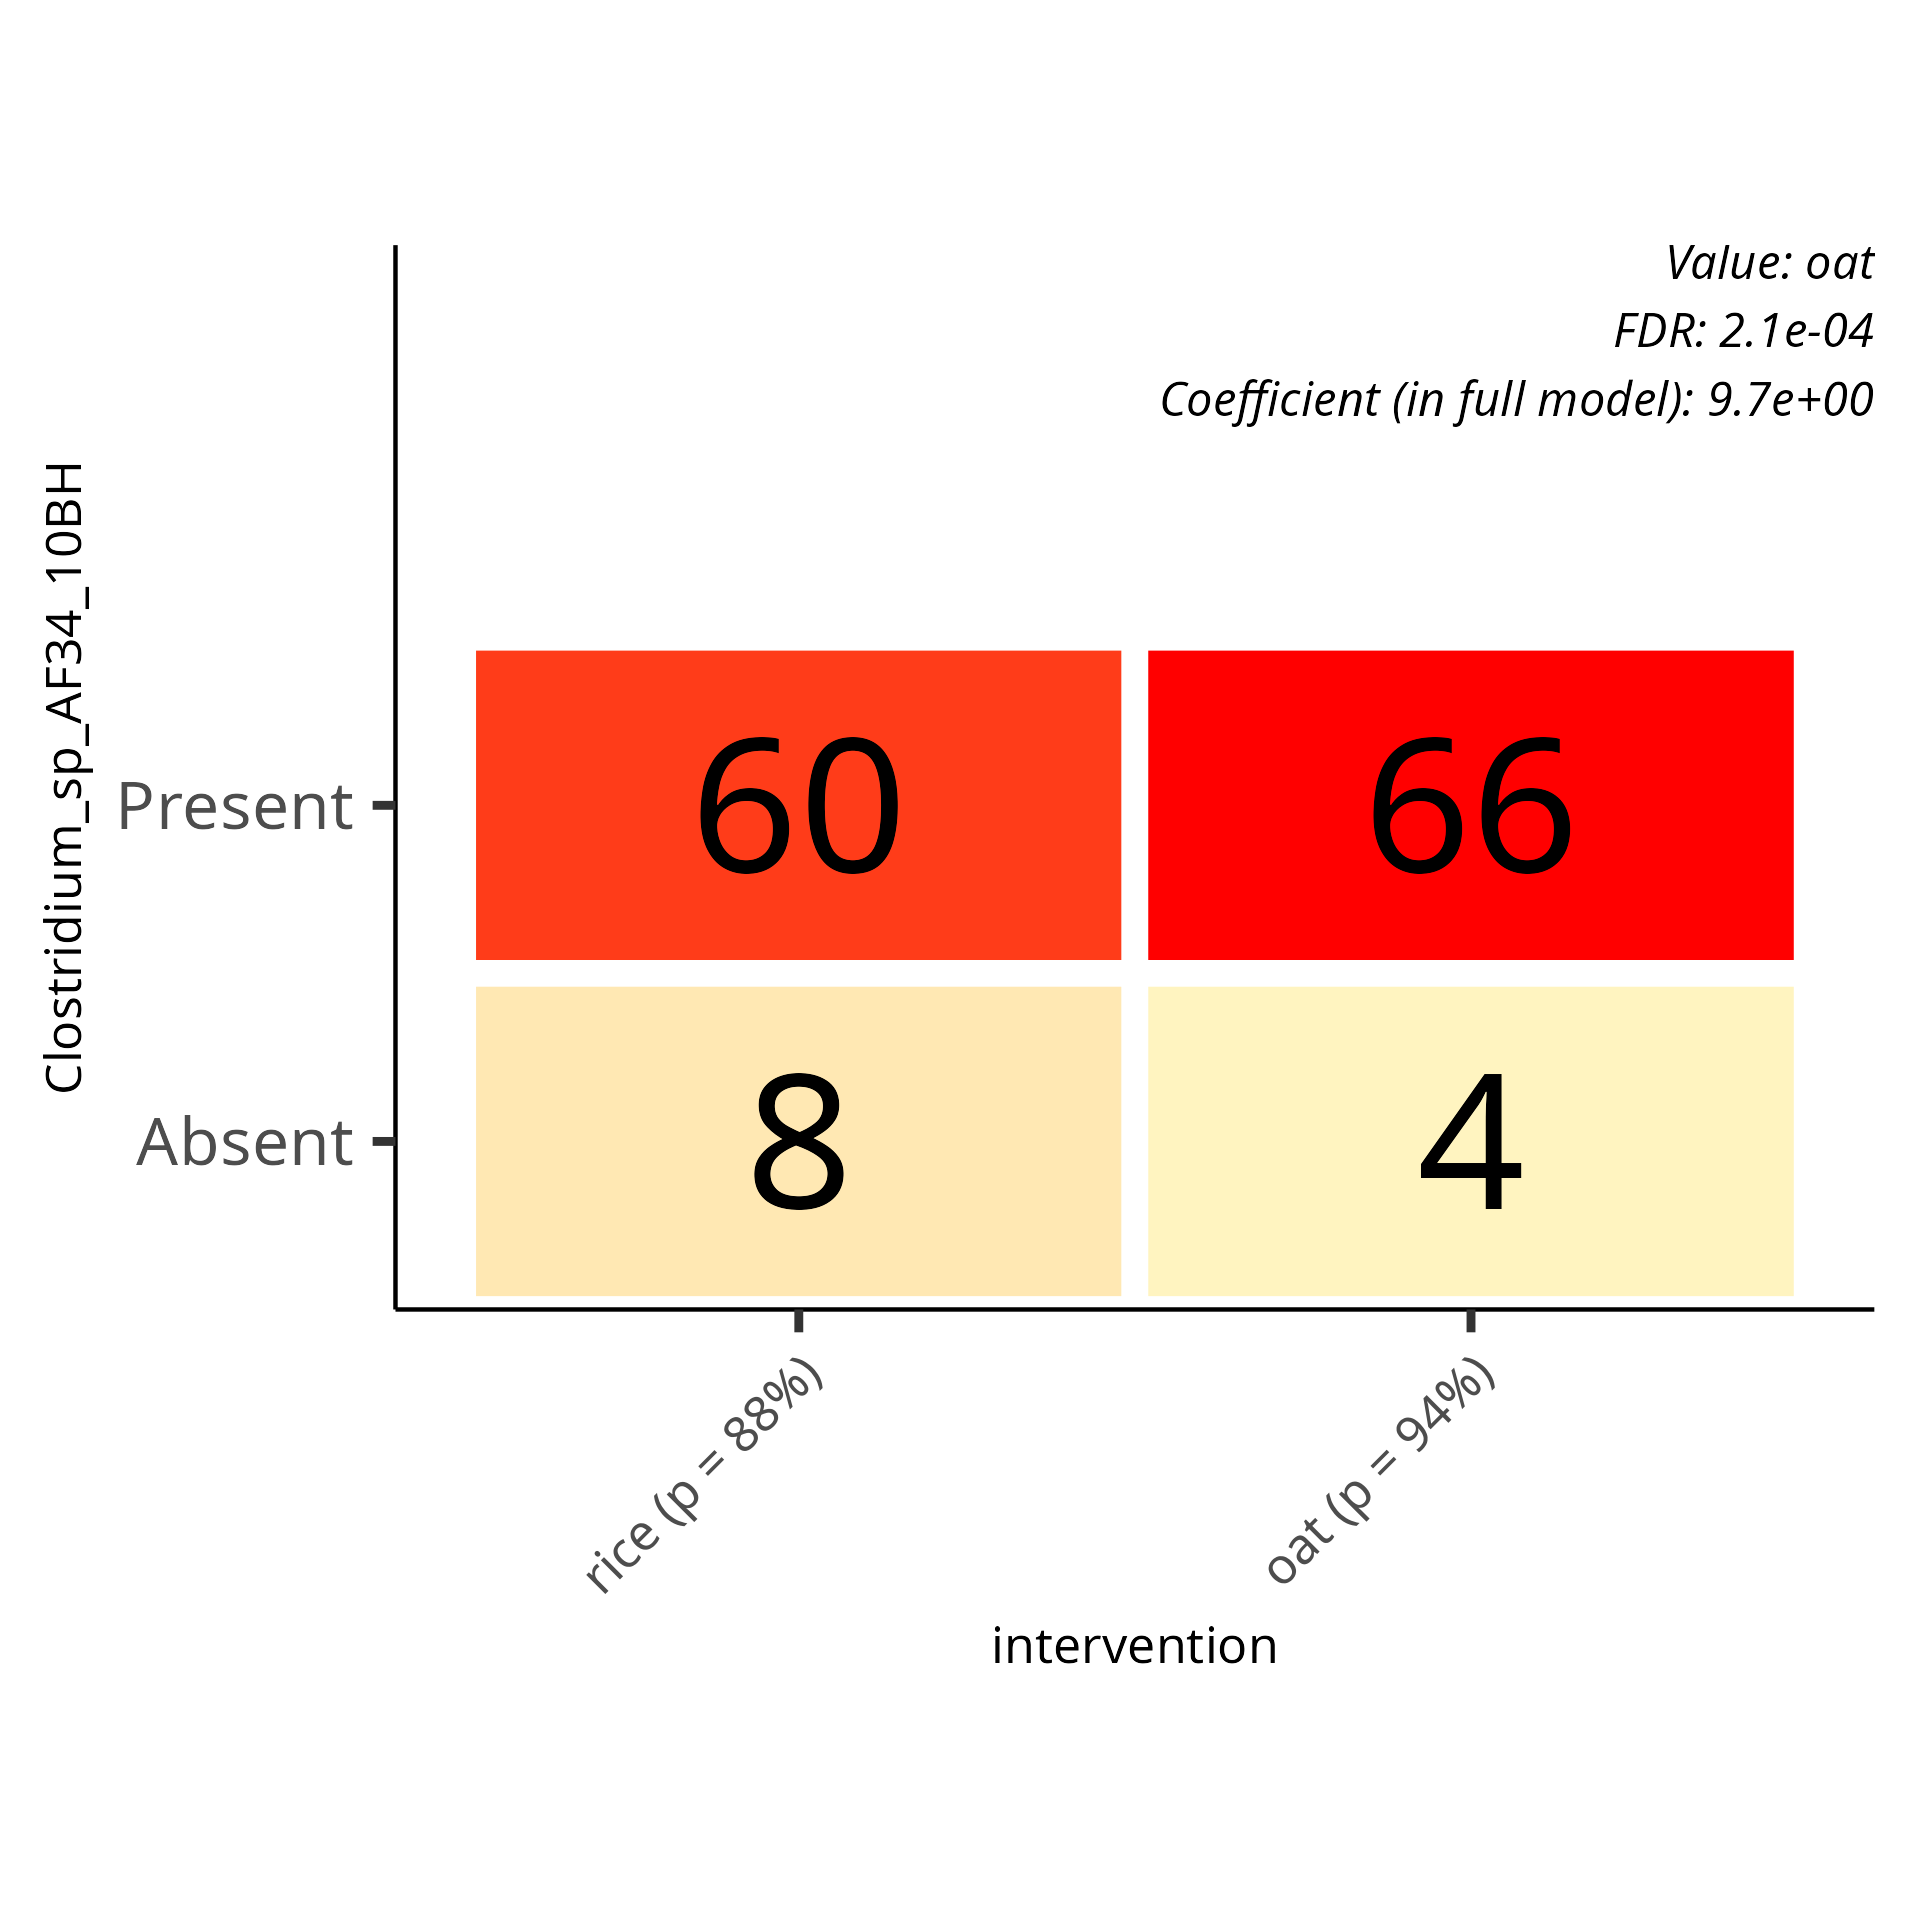
\includegraphics{../../output/daa/daa_taxa/species/figures/association_plots/intervention/logistic/intervention_Clostridium_sp_AF34_10BH_logistic.png}\\
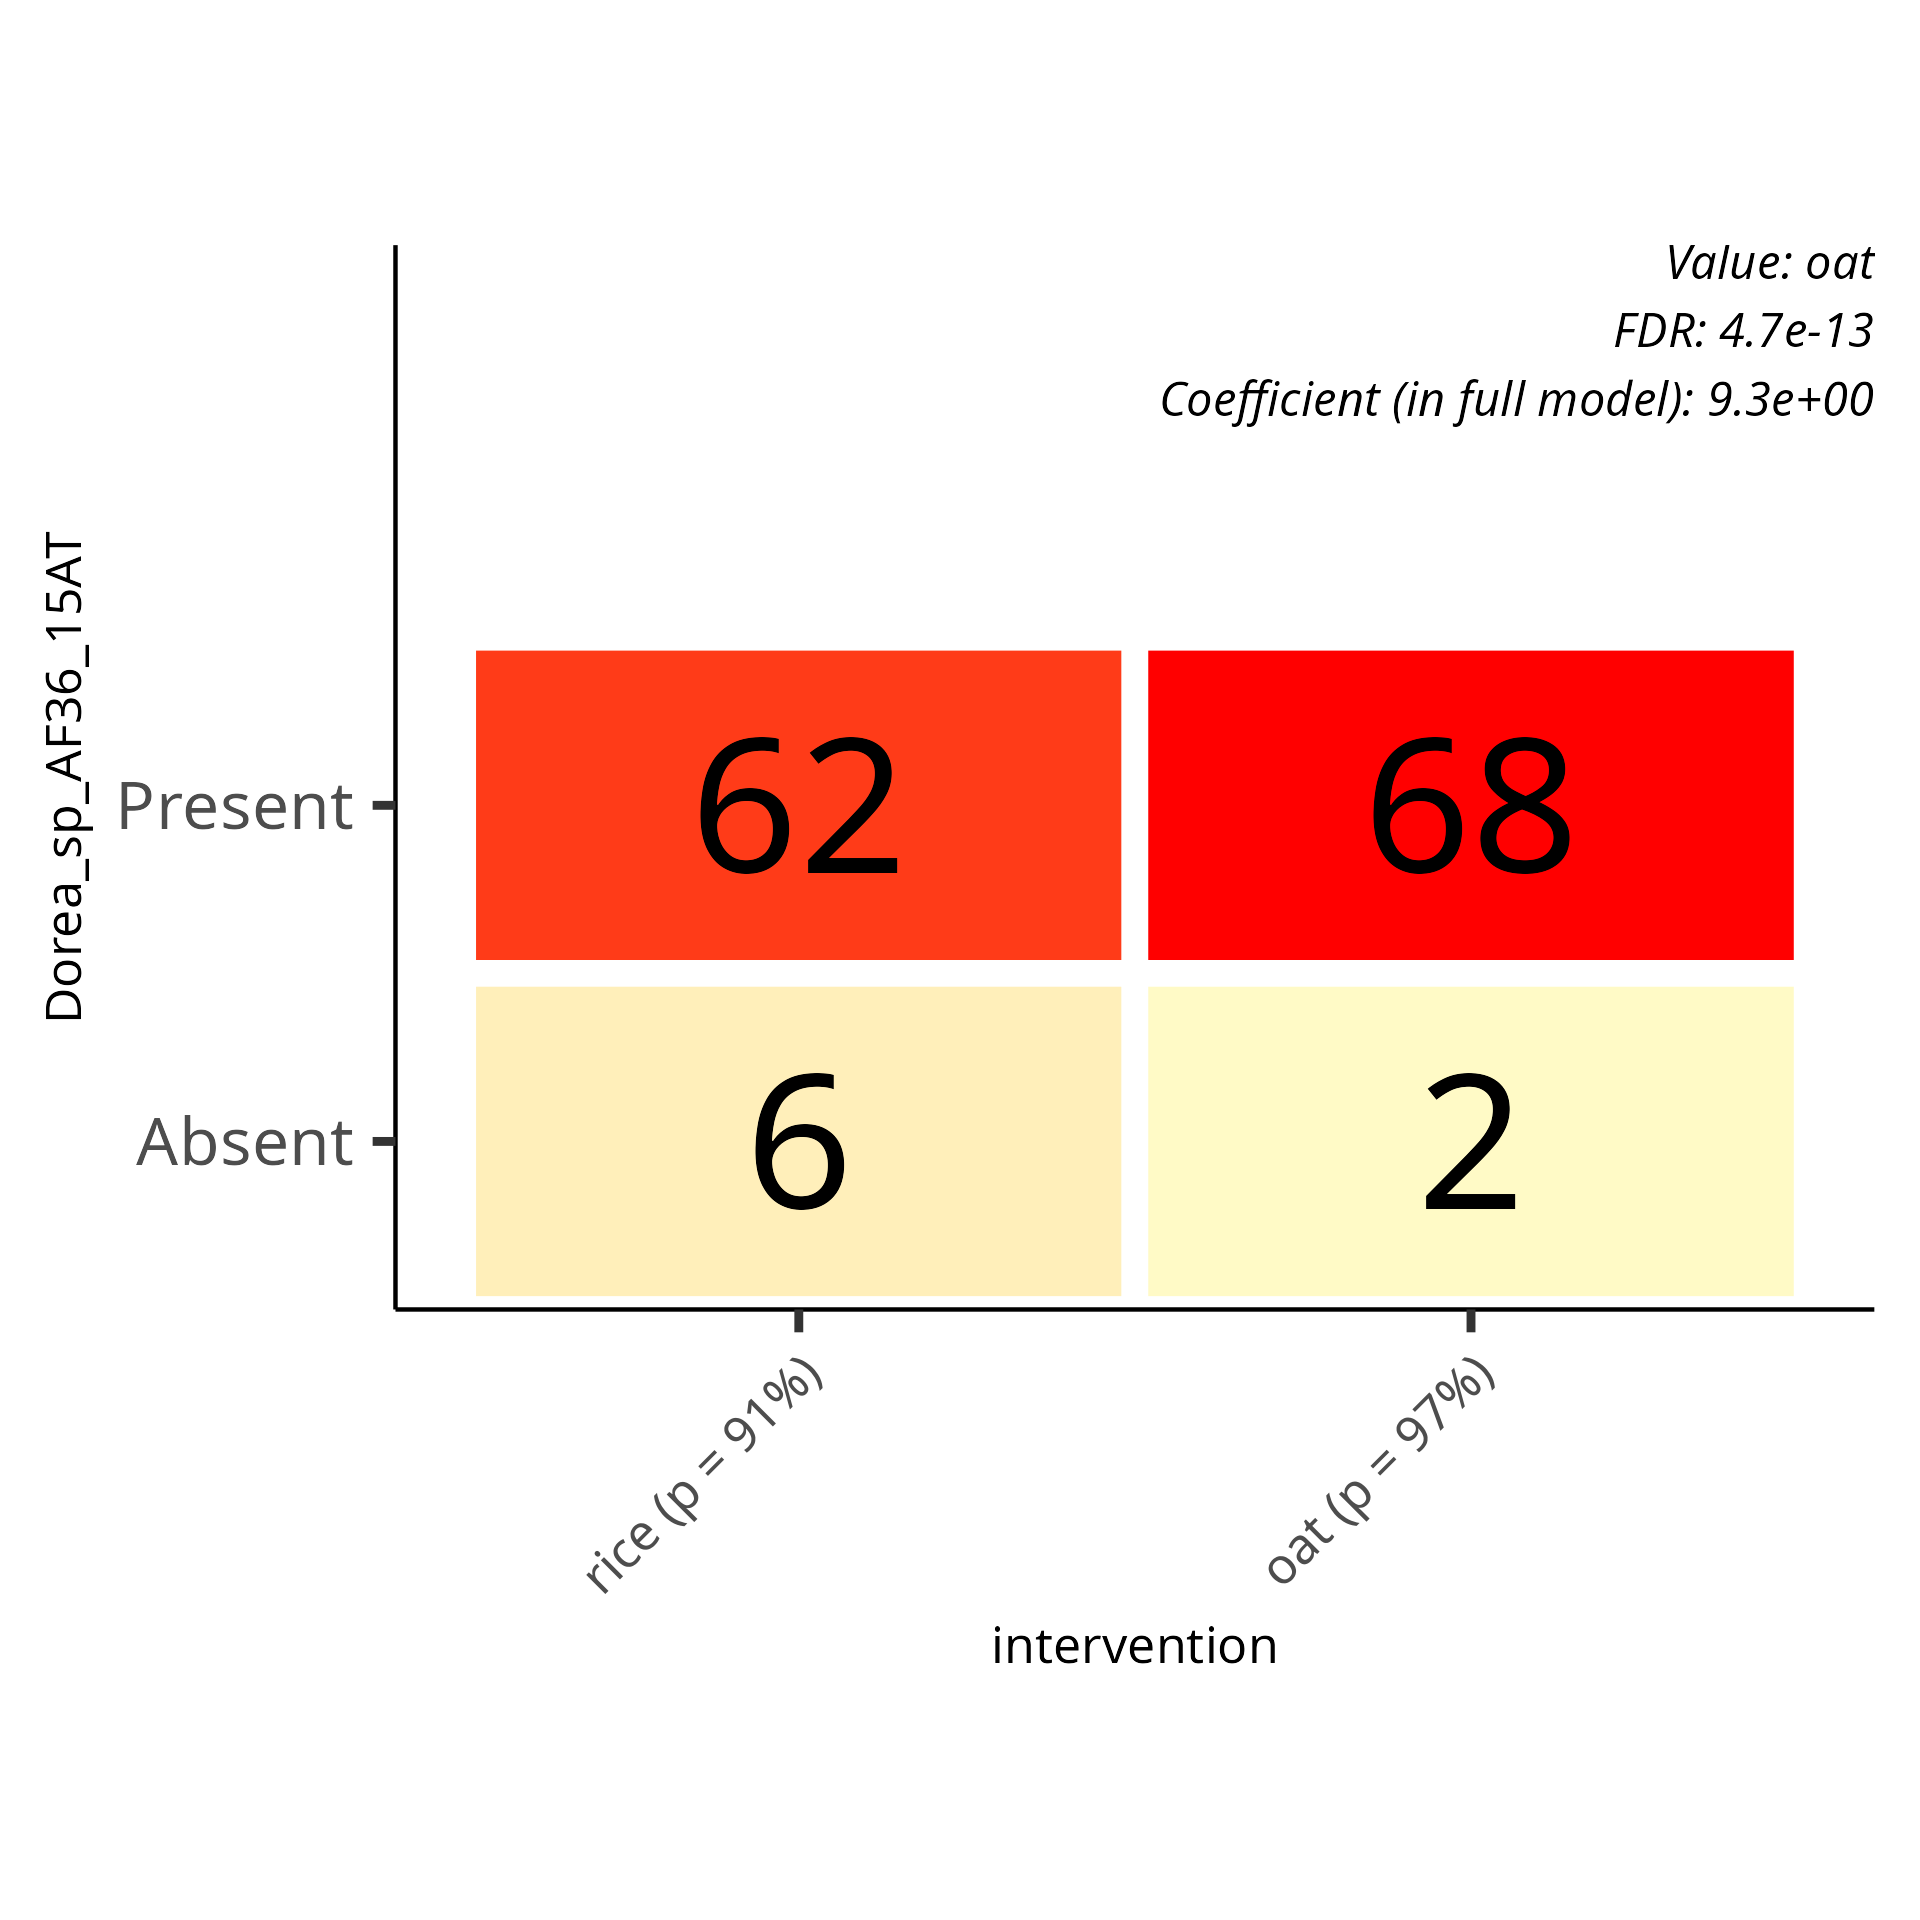
\includegraphics{../../output/daa/daa_taxa/species/figures/association_plots/intervention/logistic/intervention_Dorea_sp_AF36_15AT_logistic.png}\\
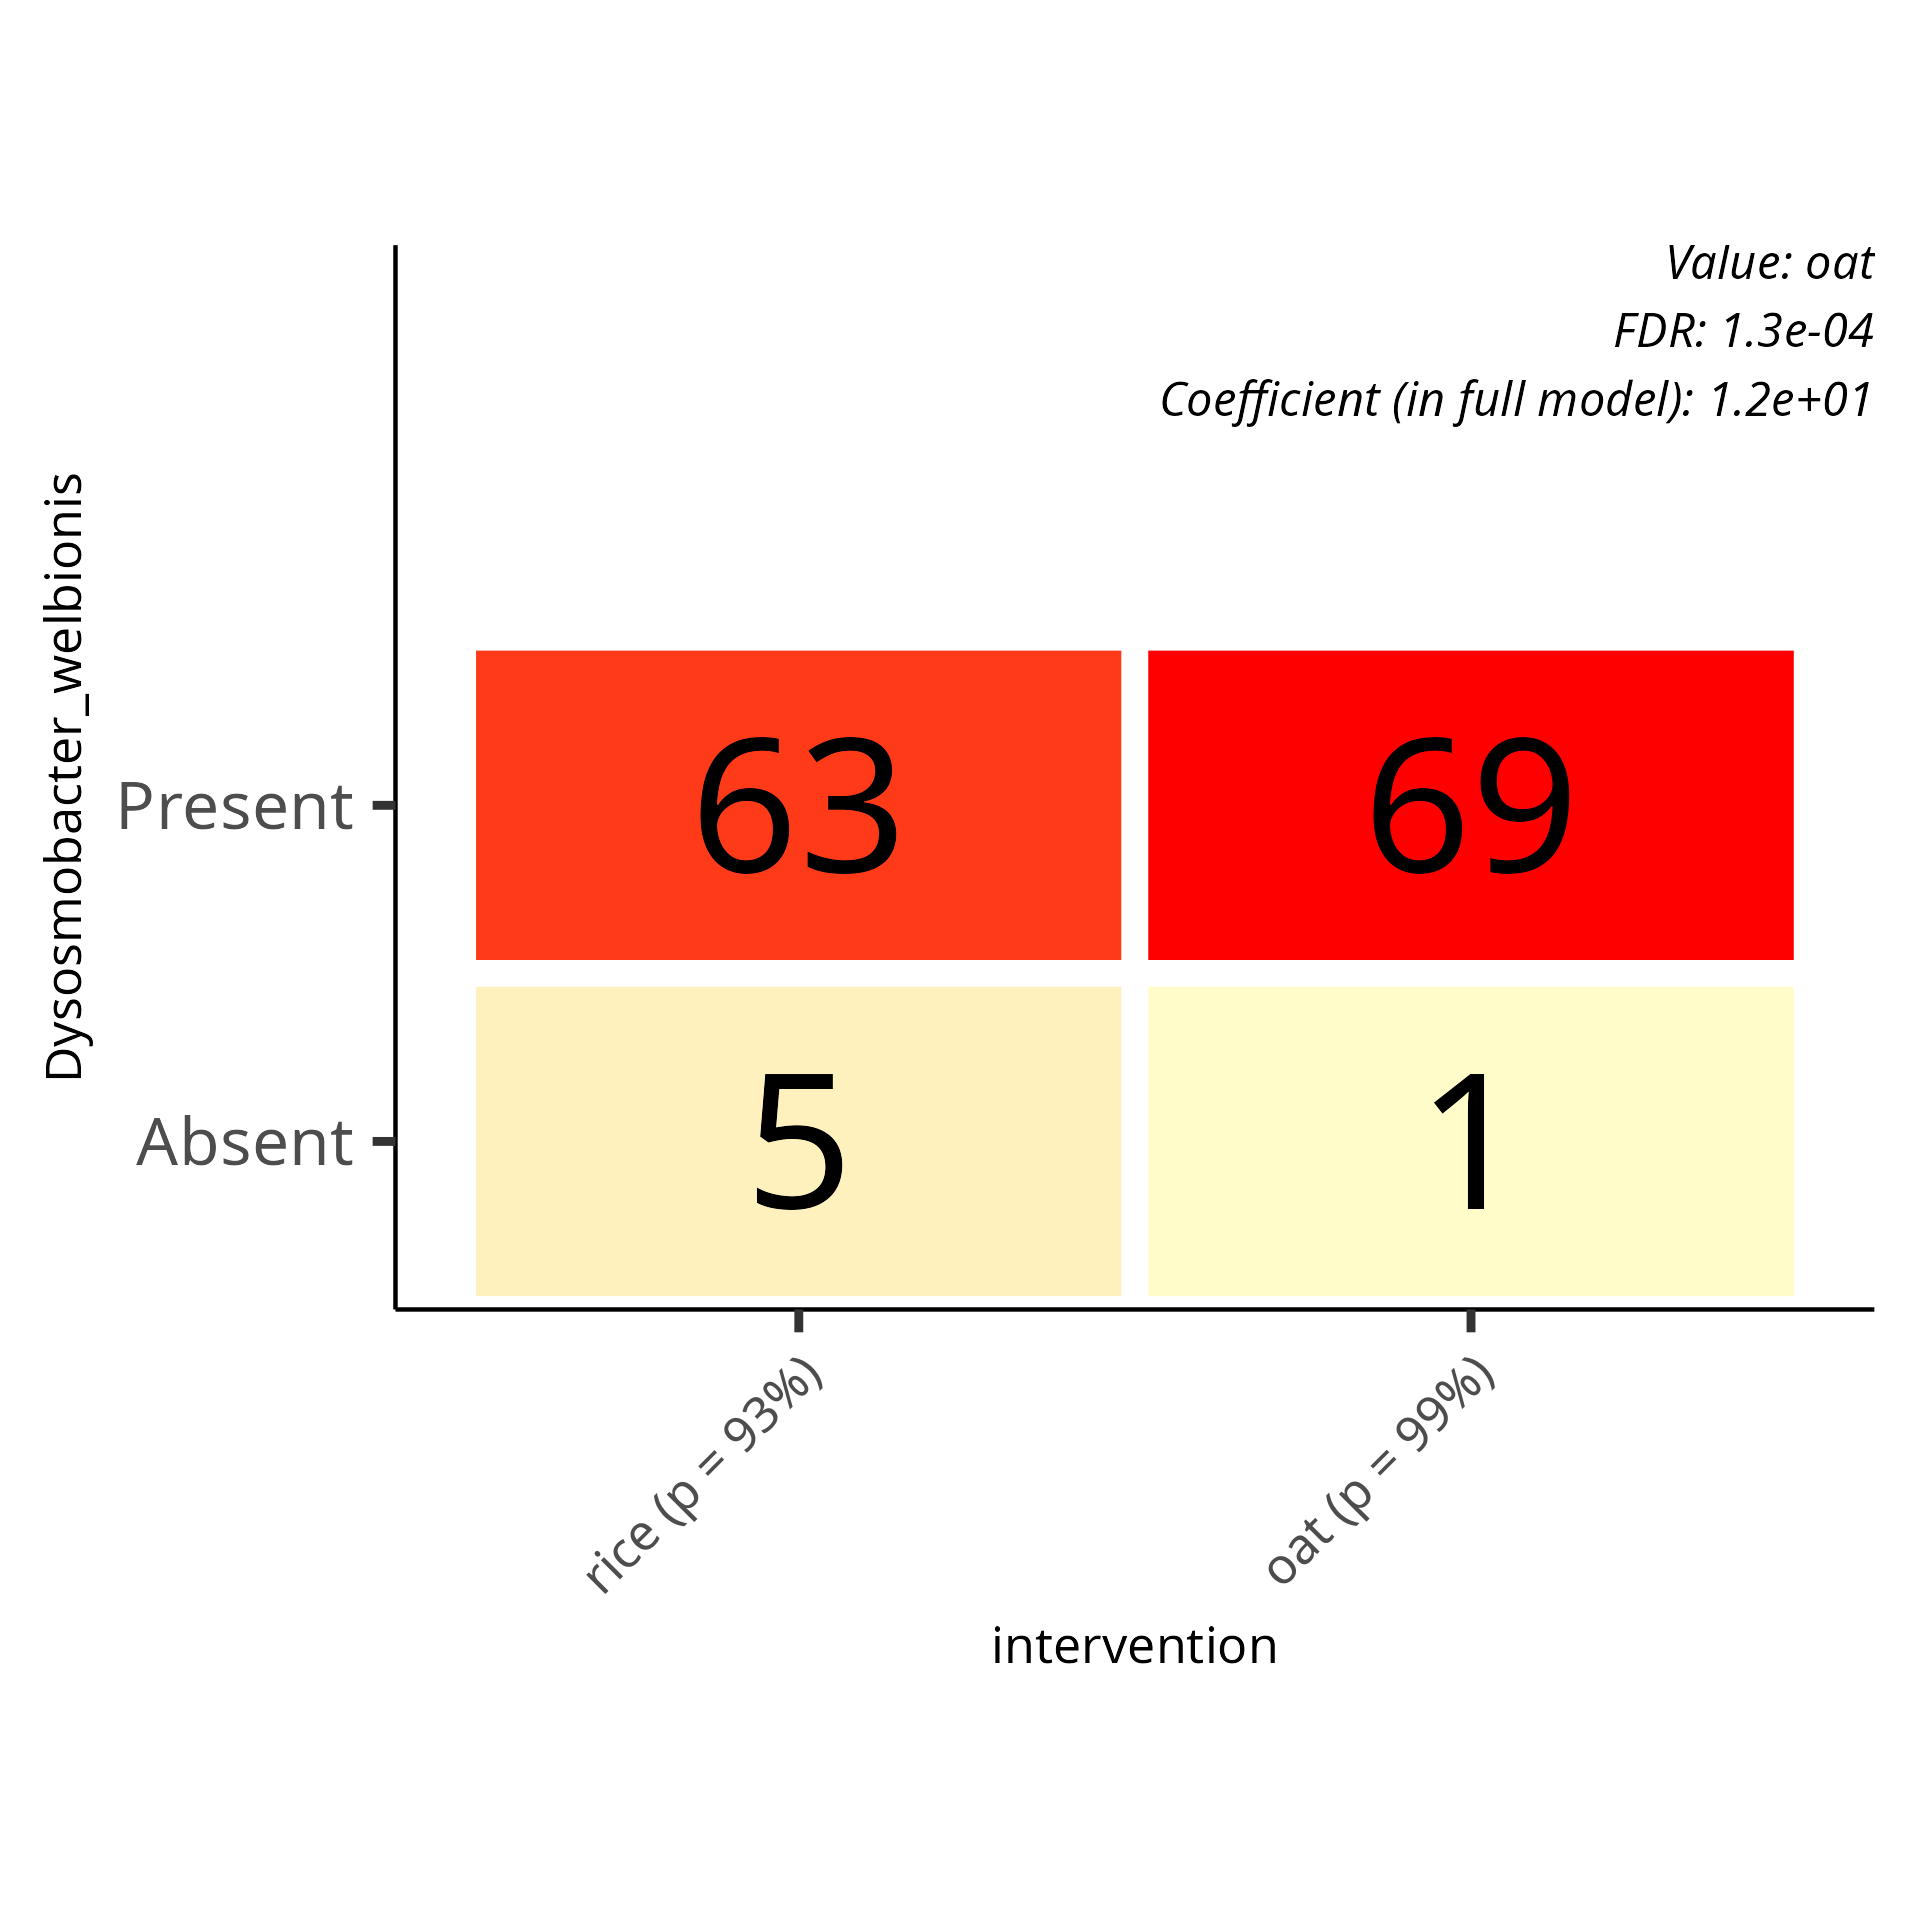
\includegraphics{../../output/daa/daa_taxa/species/figures/association_plots/intervention/logistic/intervention_Dysosmobacter_welbionis_logistic.png}\\
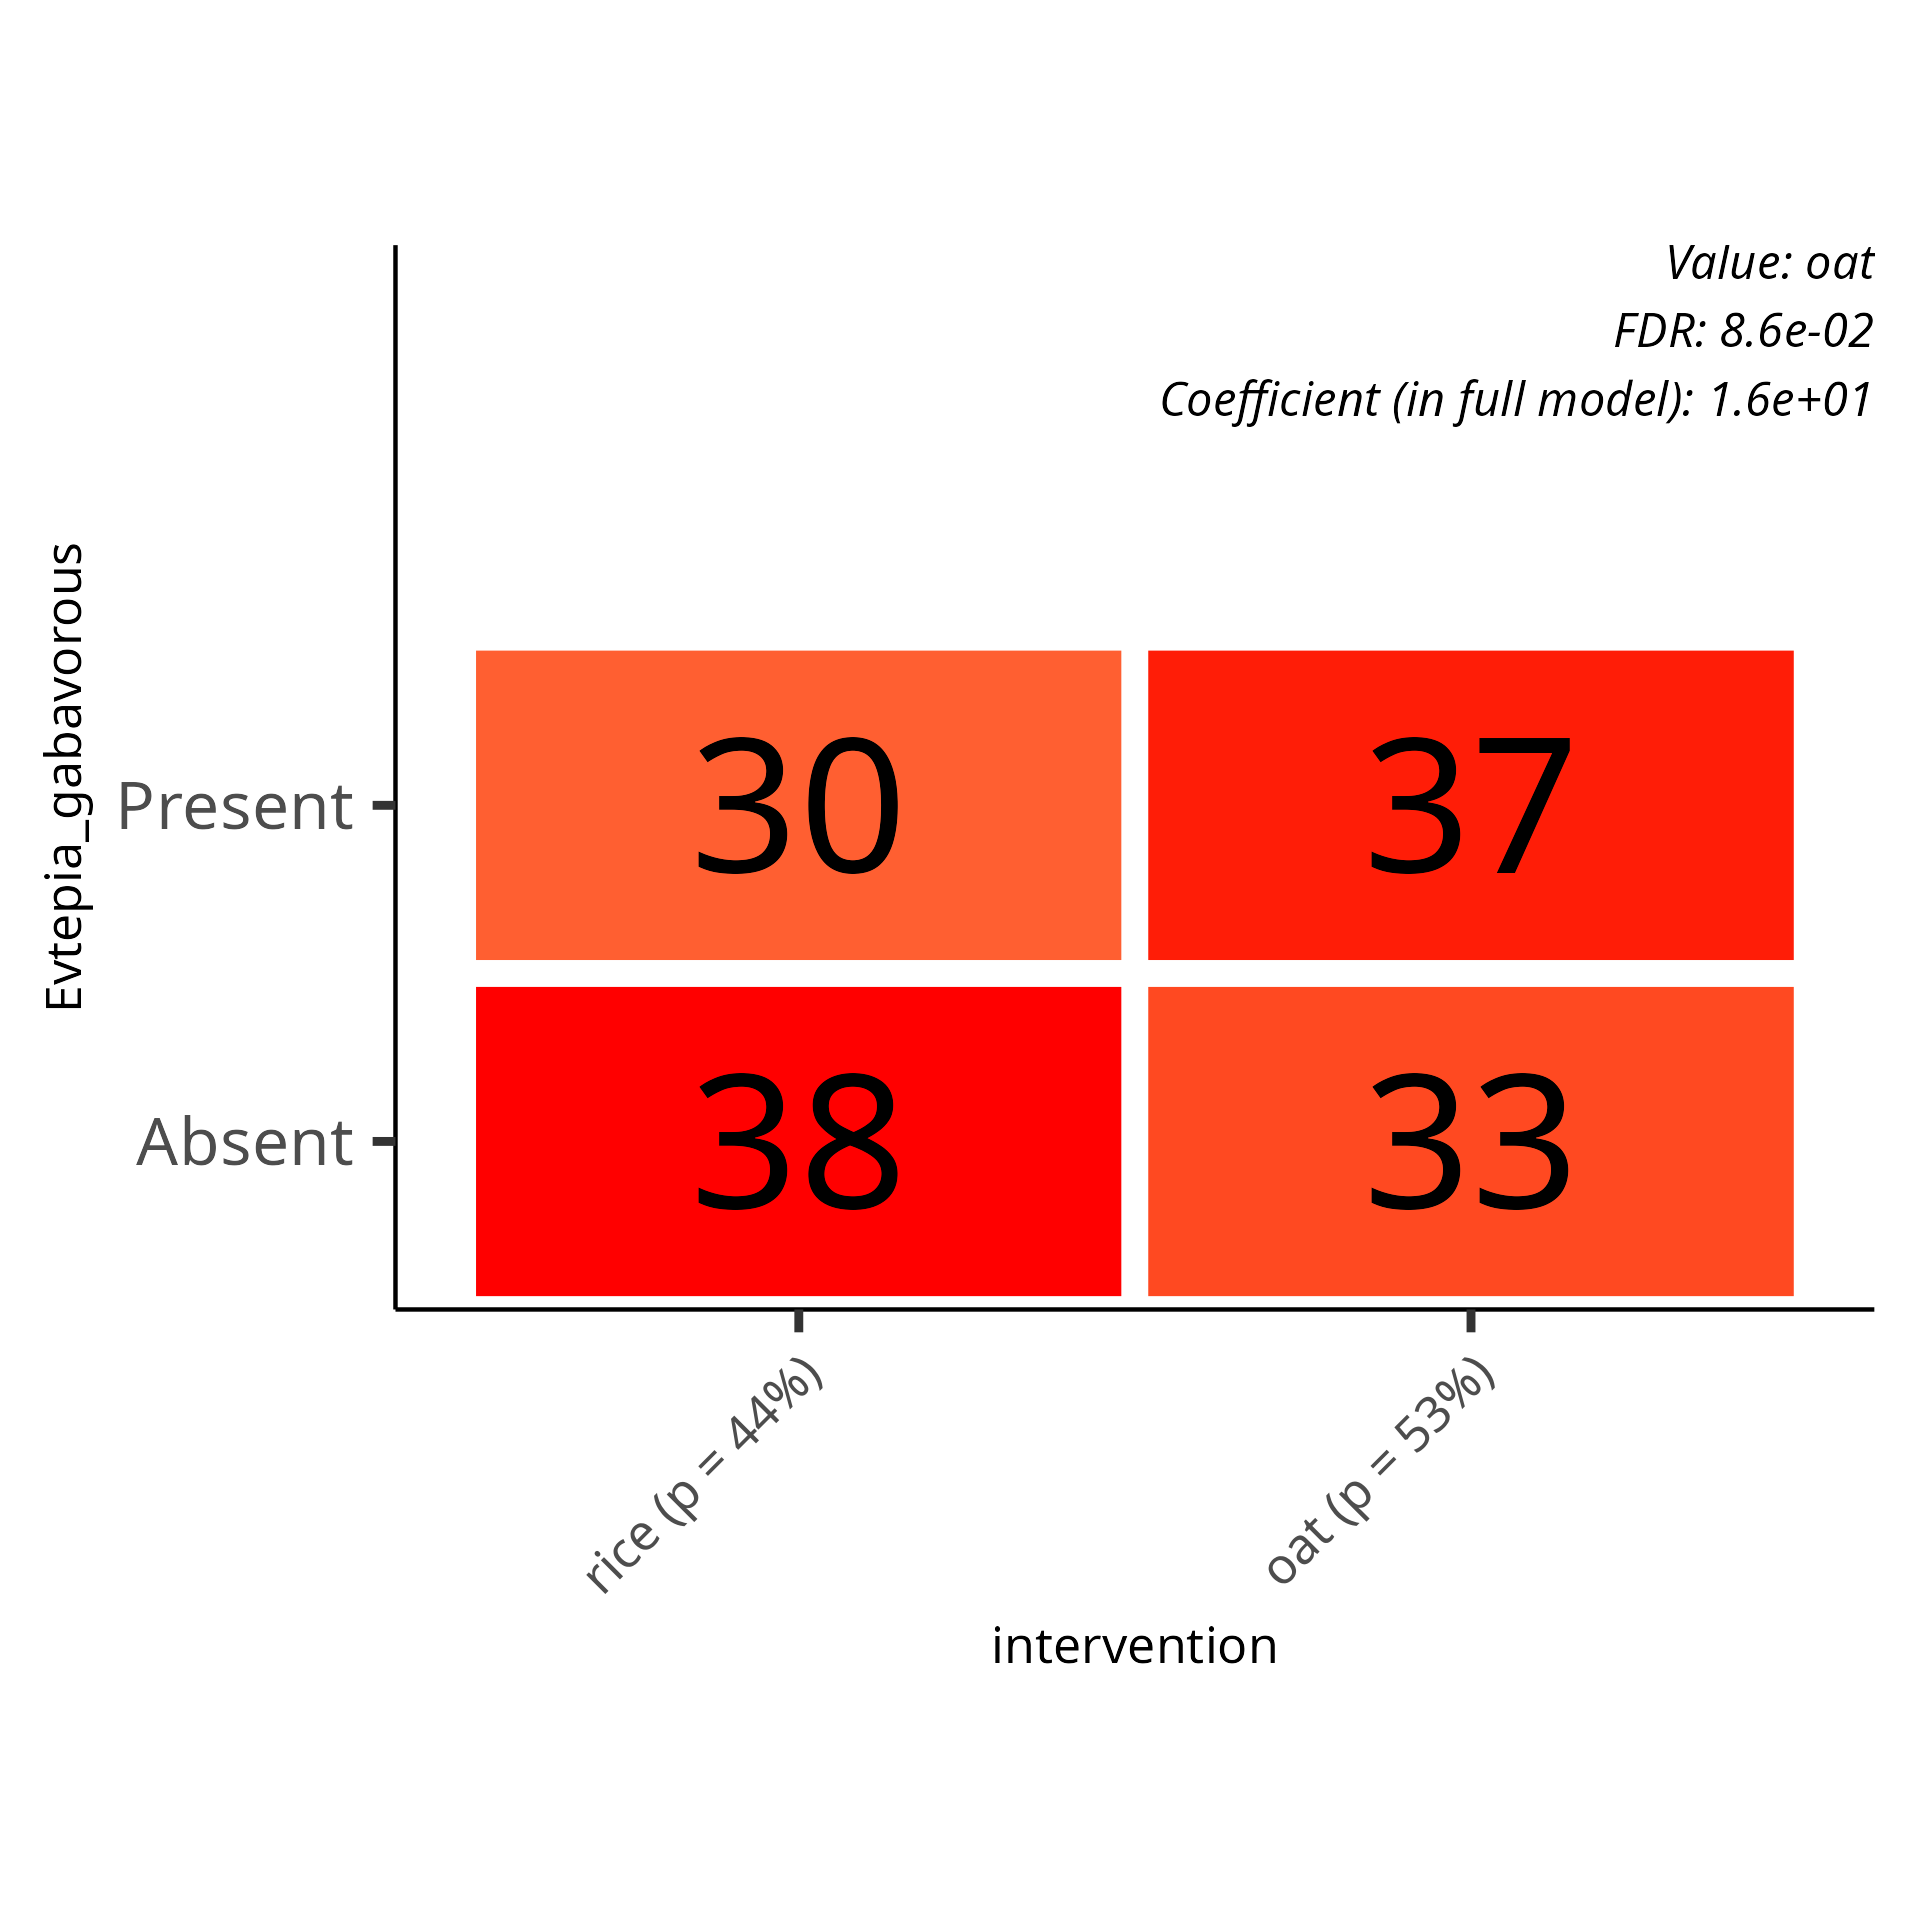
\includegraphics{../../output/daa/daa_taxa/species/figures/association_plots/intervention/logistic/intervention_Evtepia_gabavorous_logistic.png}\\
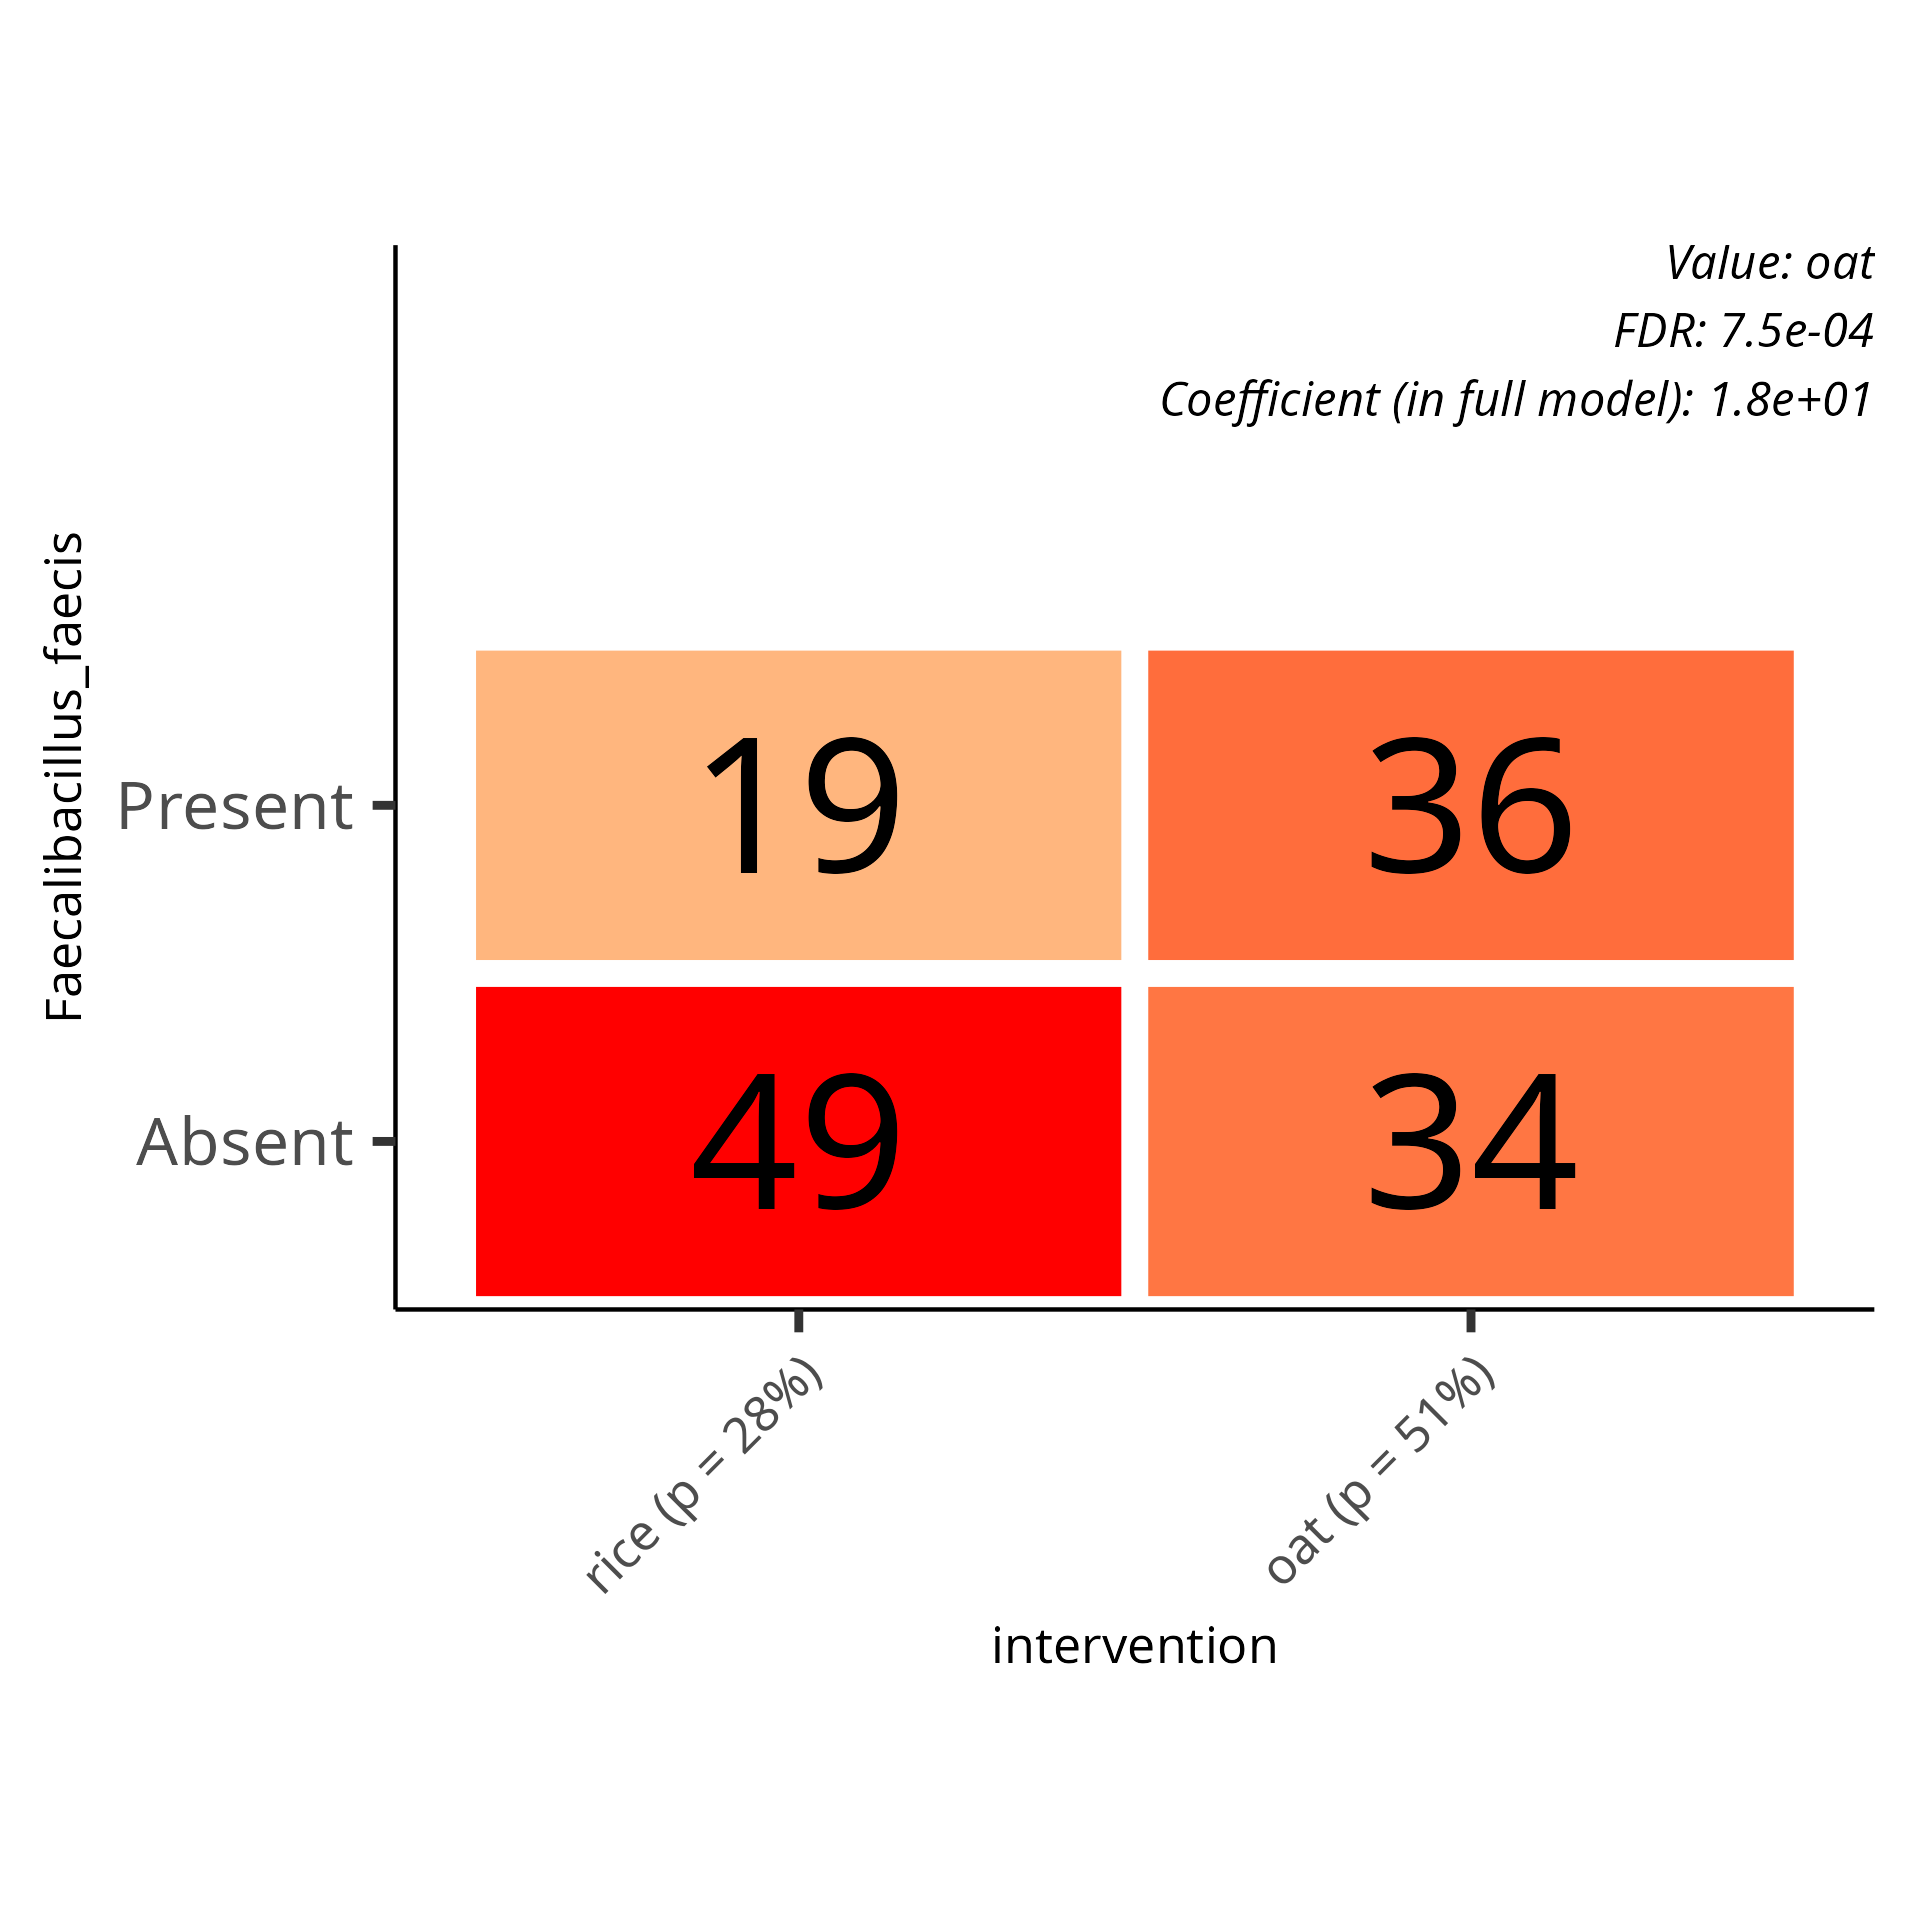
\includegraphics{../../output/daa/daa_taxa/species/figures/association_plots/intervention/logistic/intervention_Faecalibacillus_faecis_logistic.png}\\
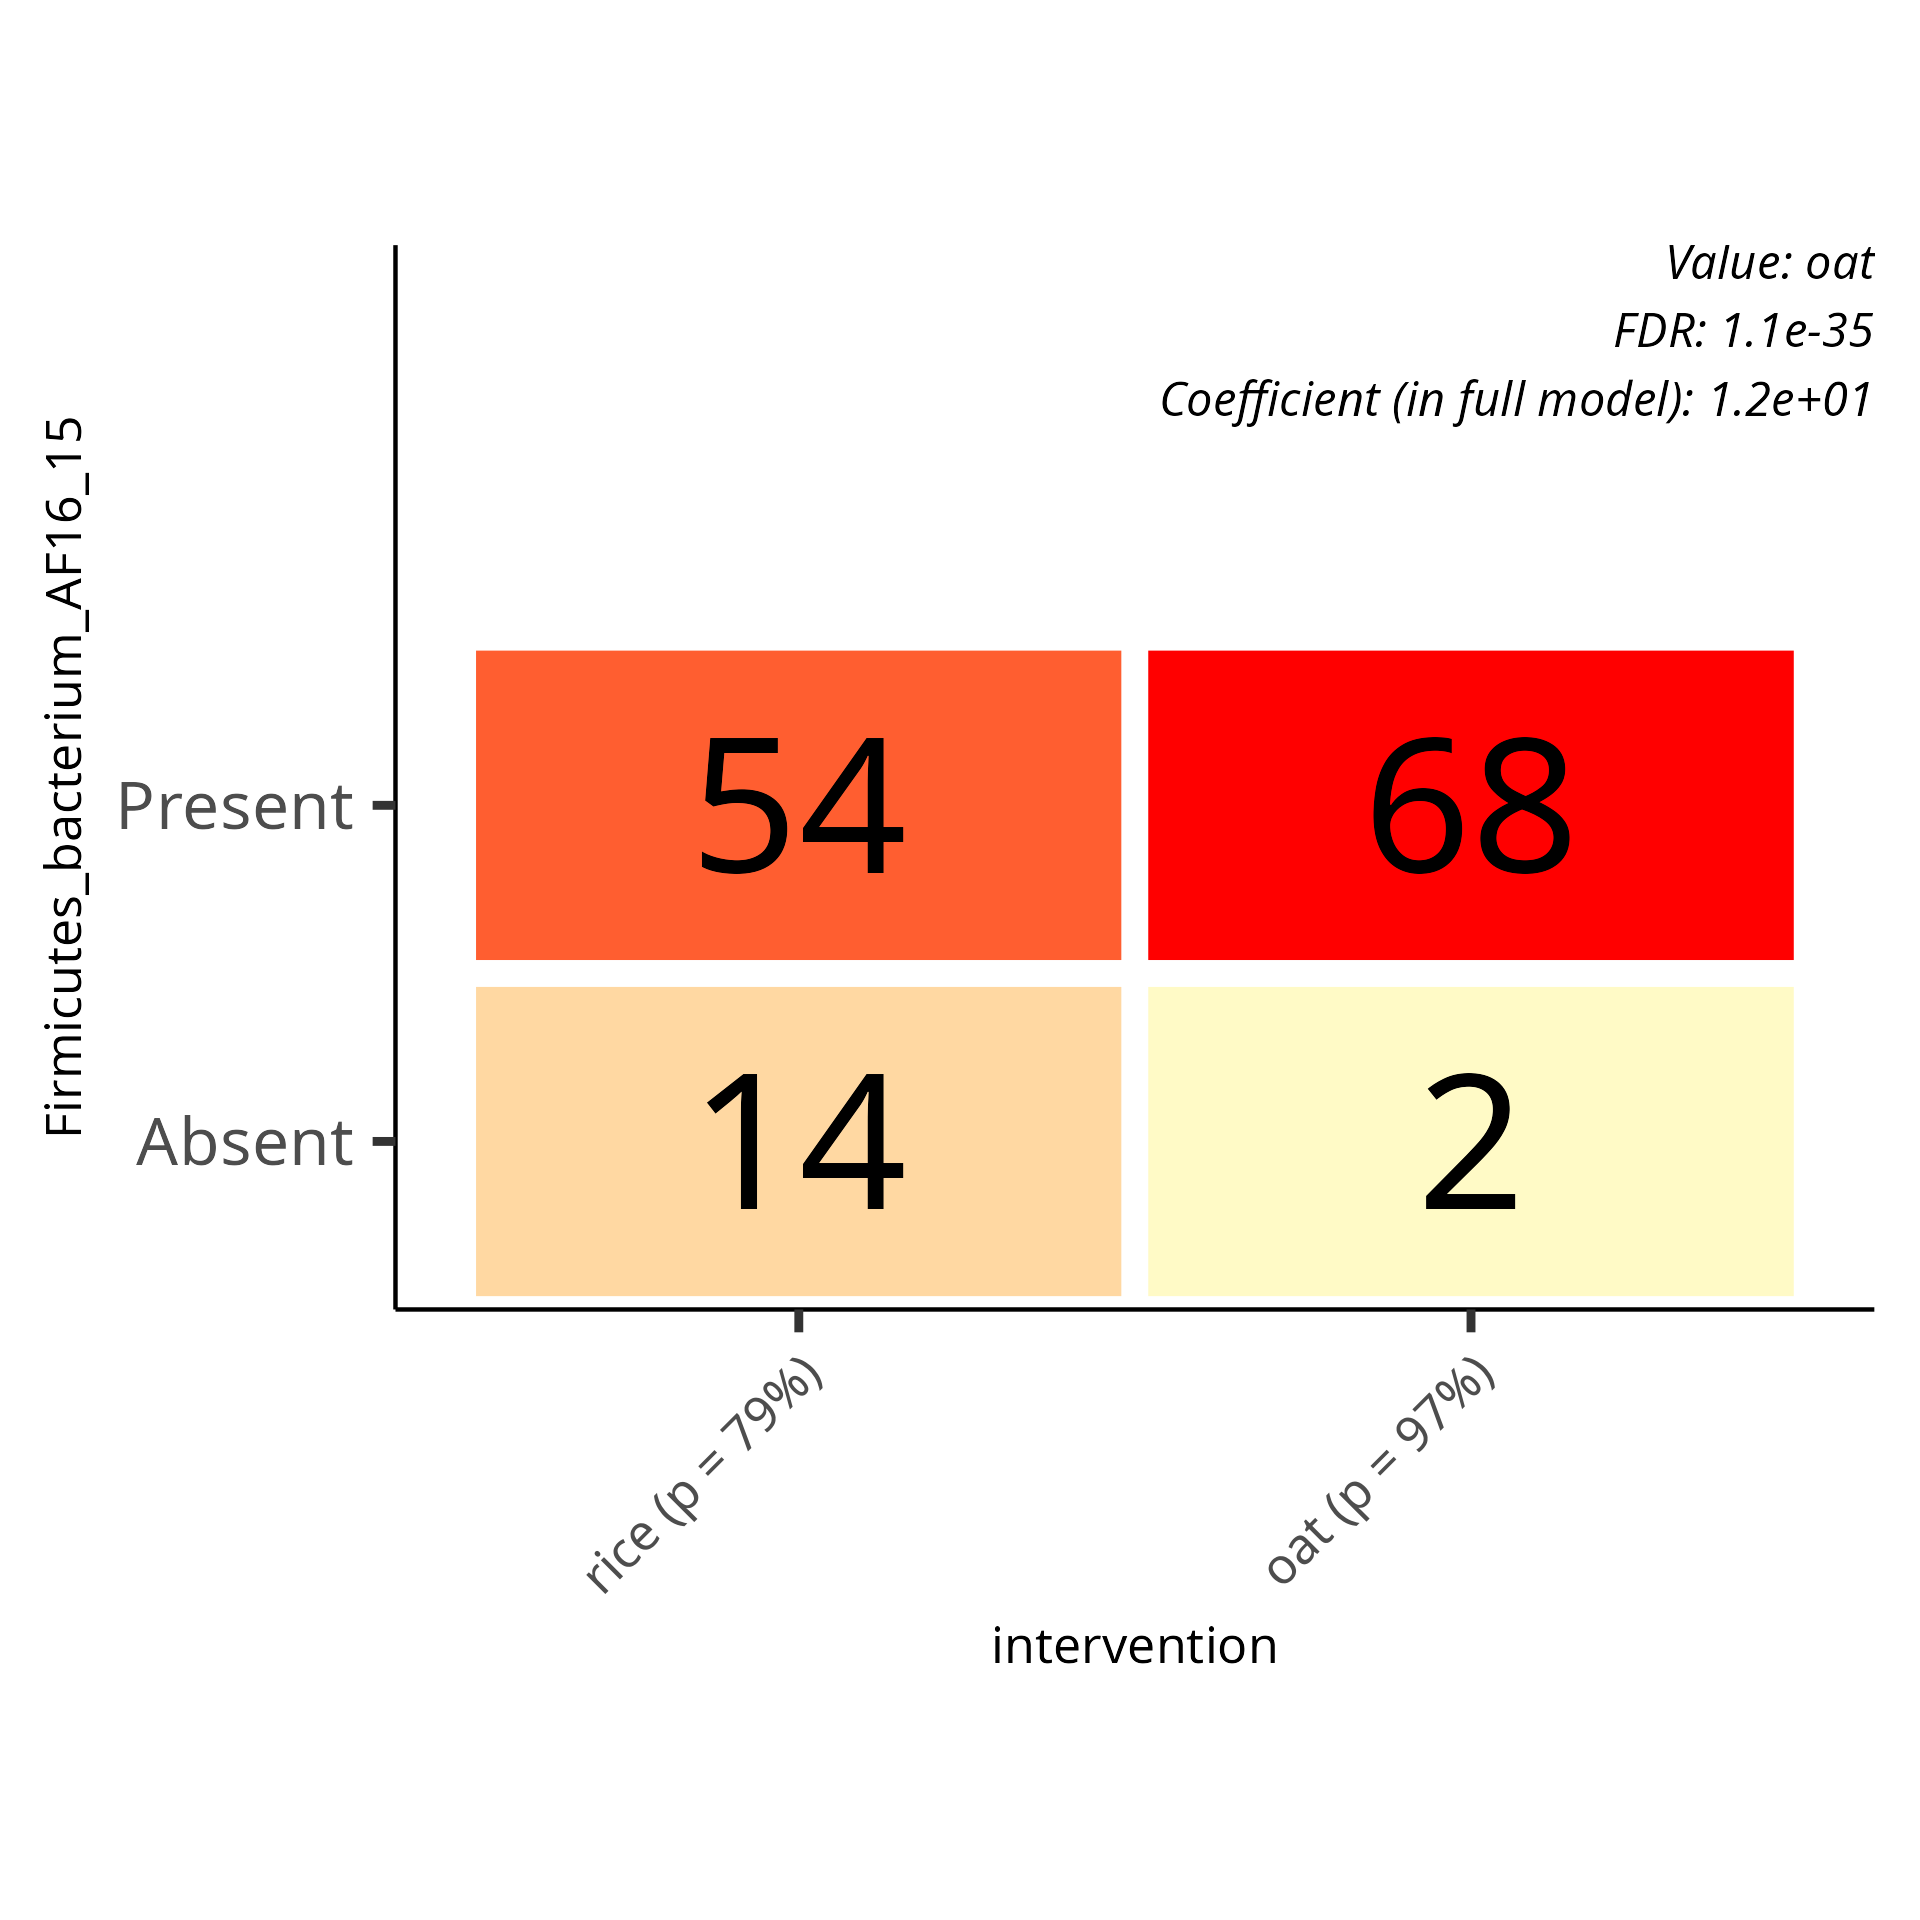
\includegraphics{../../output/daa/daa_taxa/species/figures/association_plots/intervention/logistic/intervention_Firmicutes_bacterium_AF16_15_logistic.png}\\
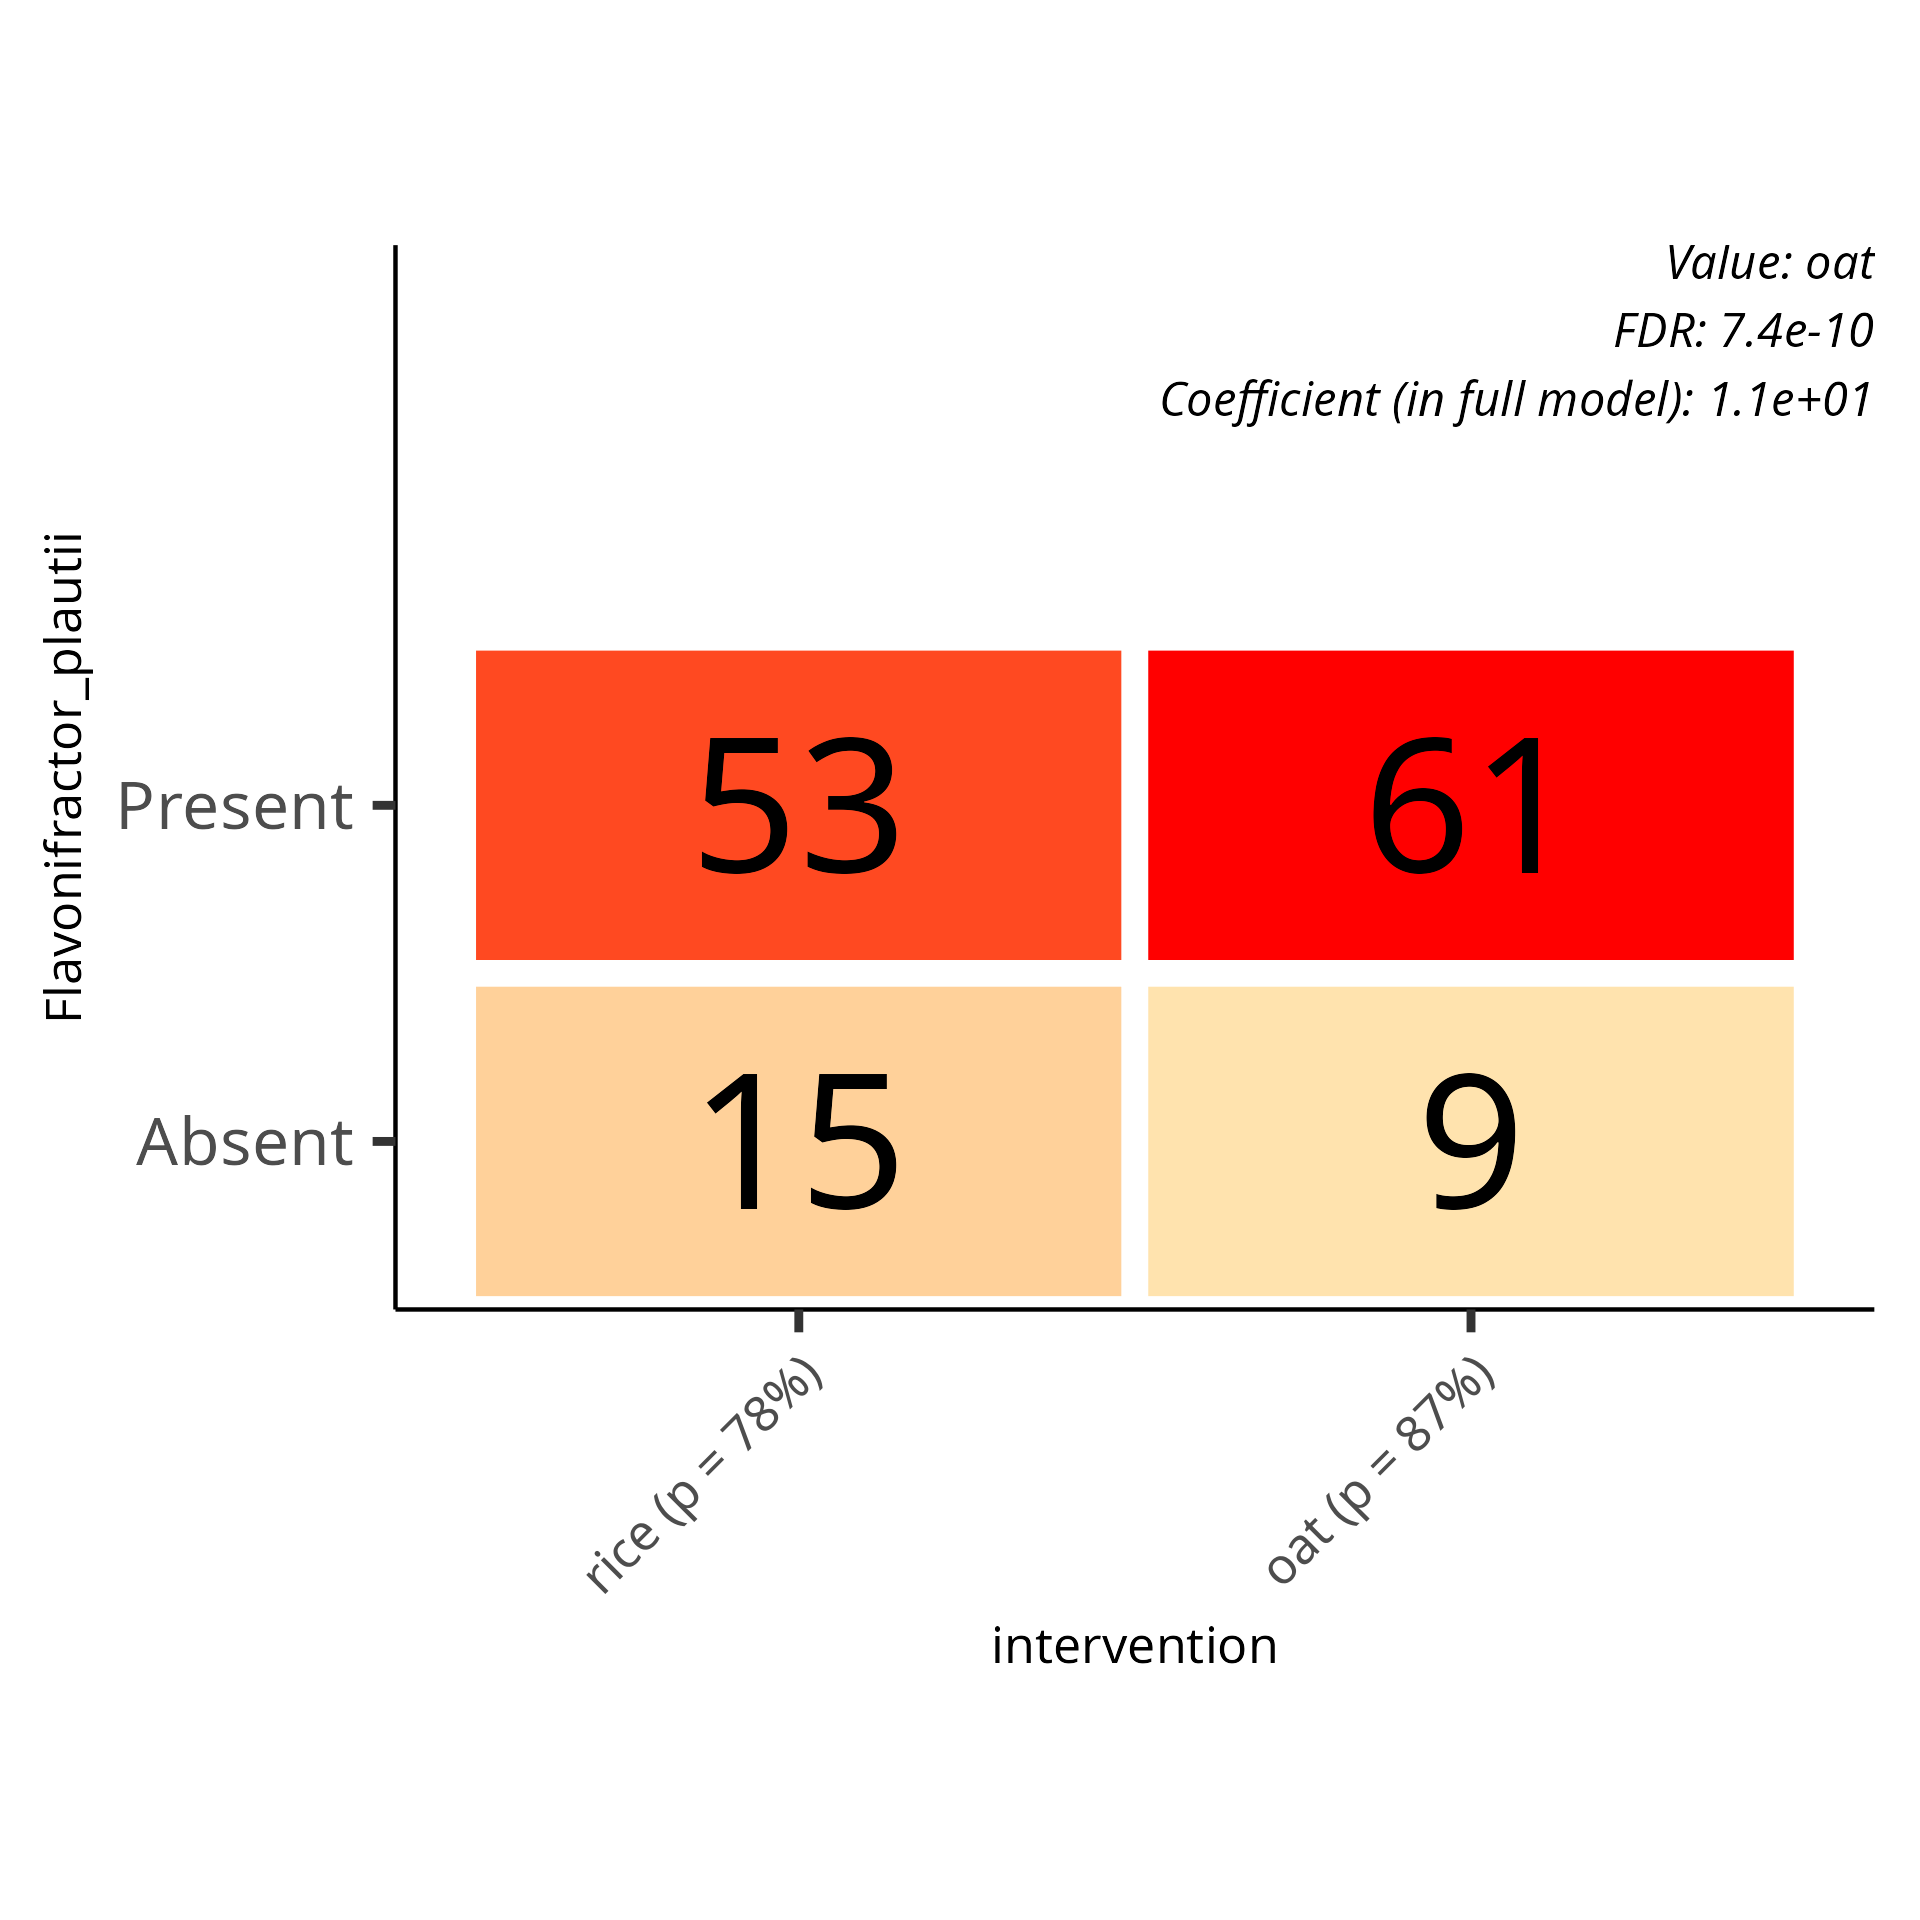
\includegraphics{../../output/daa/daa_taxa/species/figures/association_plots/intervention/logistic/intervention_Flavonifractor_plautii_logistic.png}\\
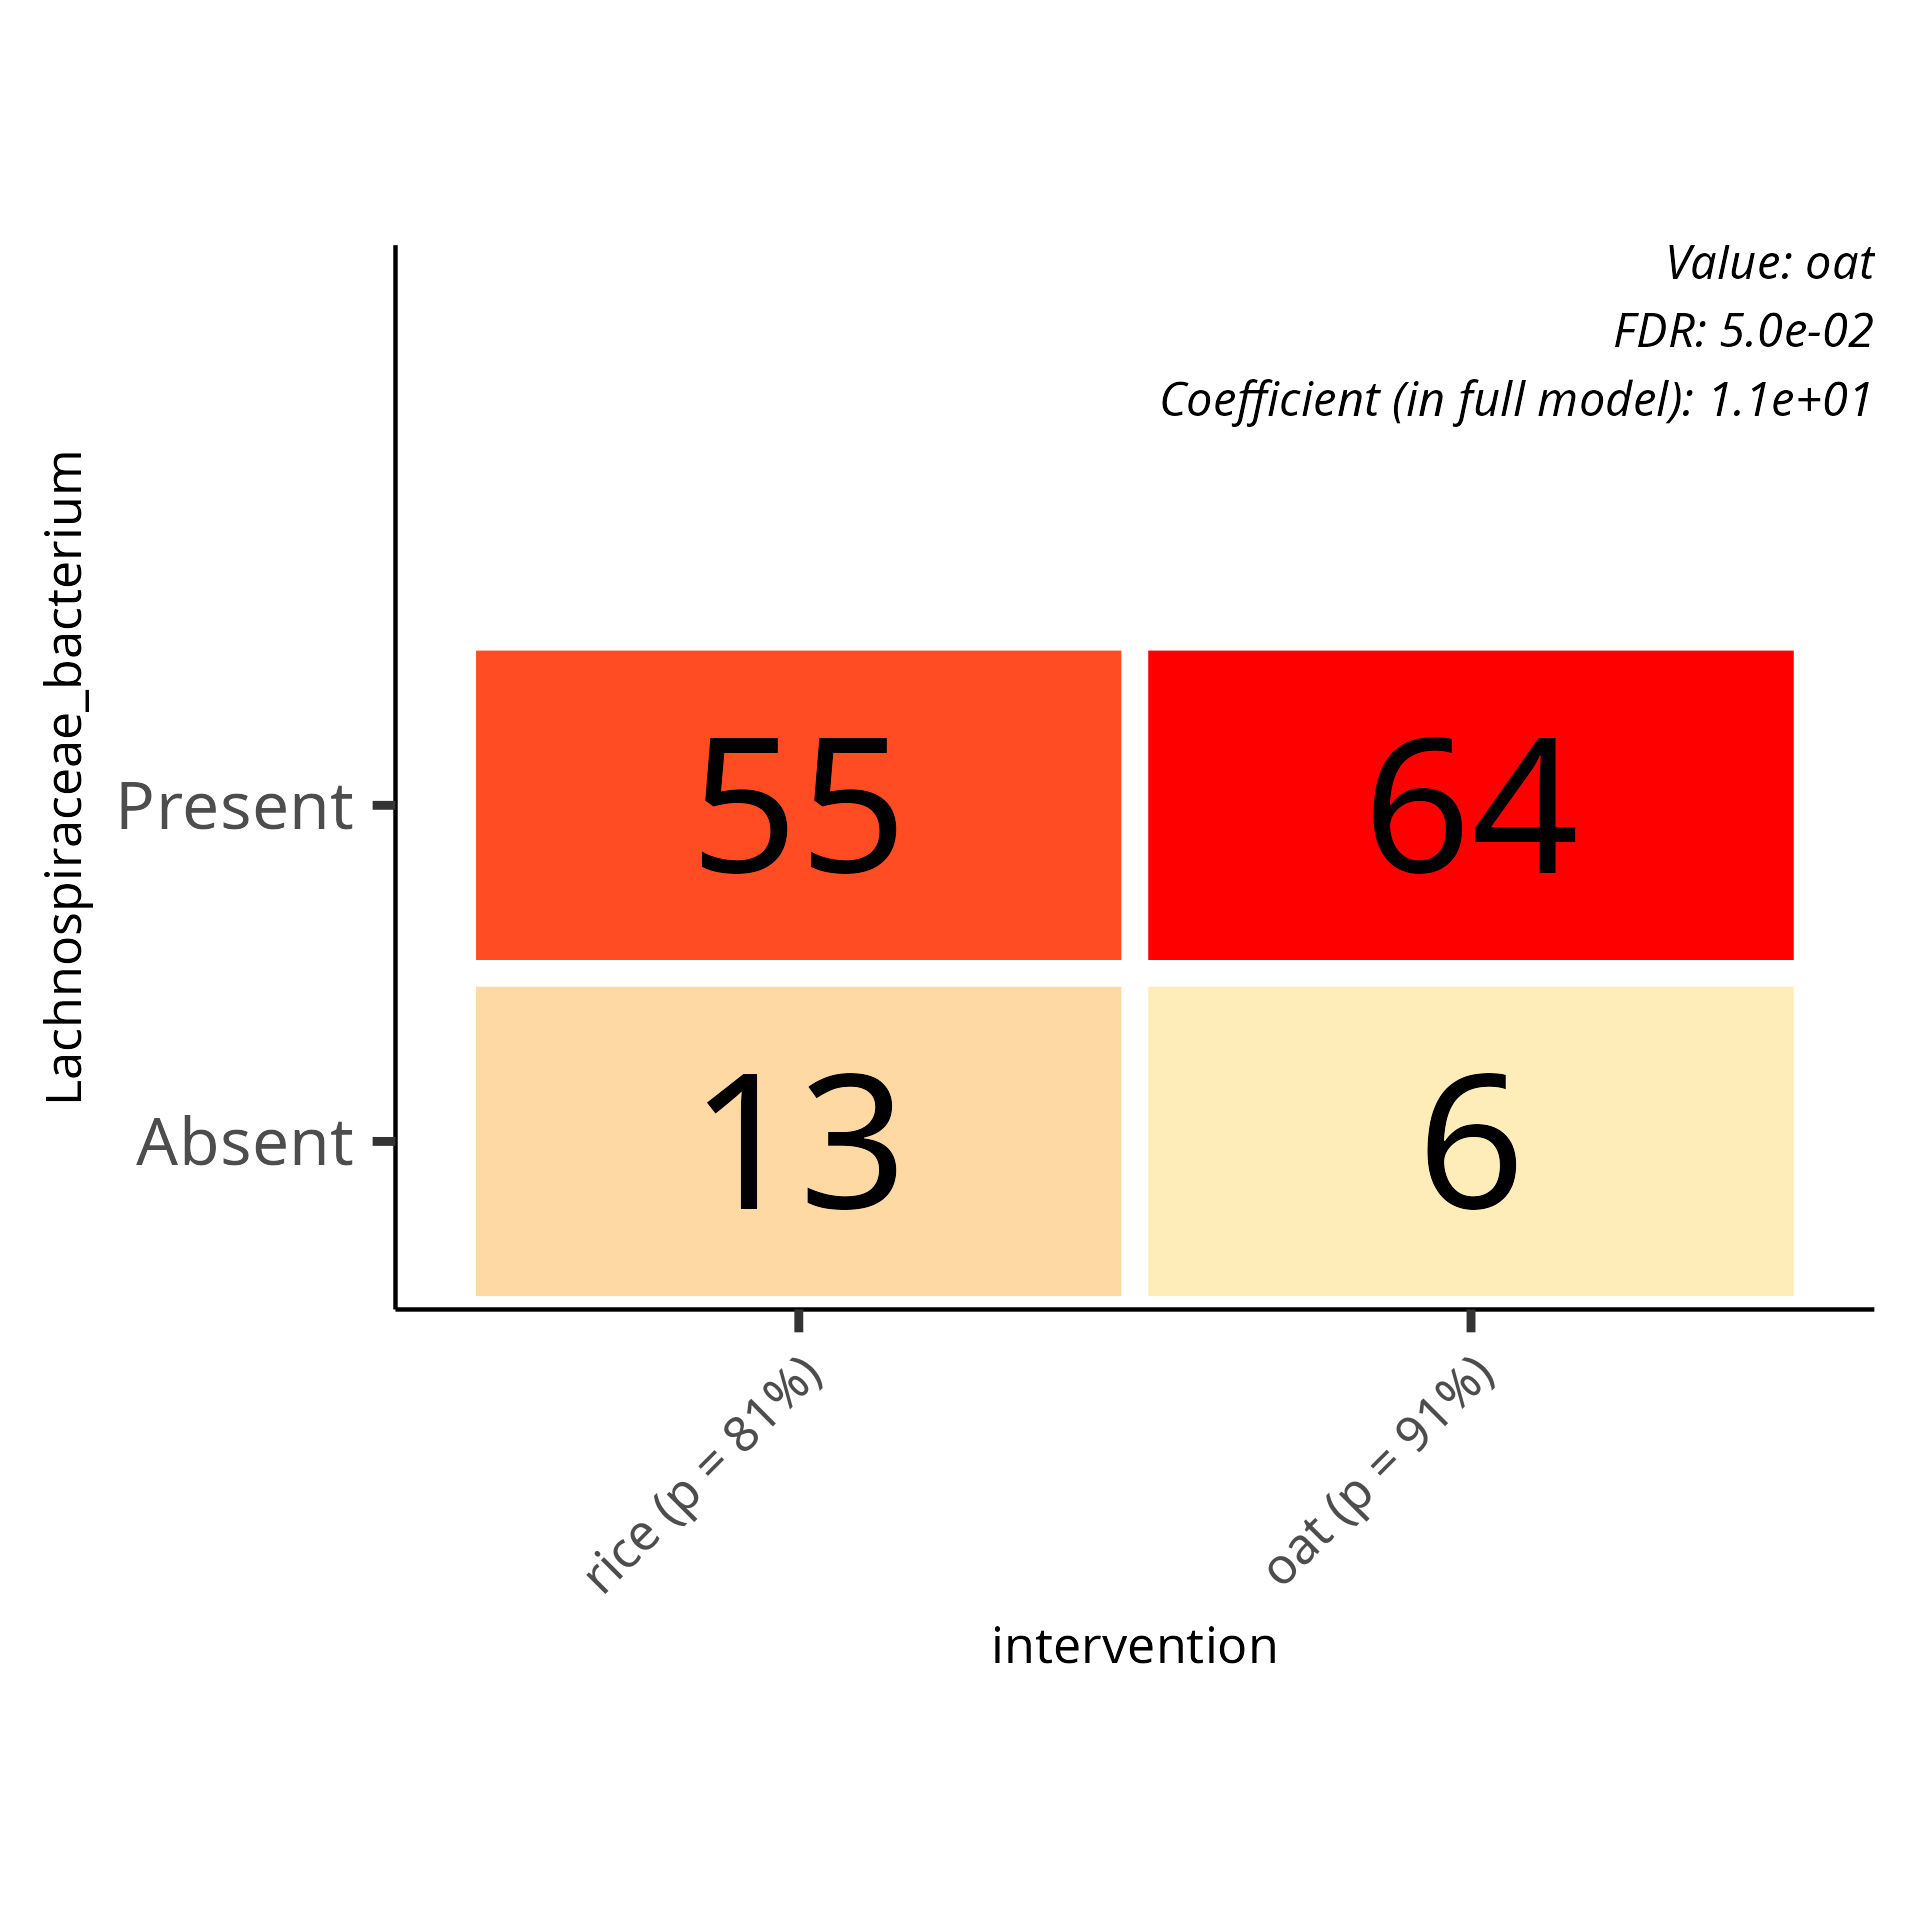
\includegraphics{../../output/daa/daa_taxa/species/figures/association_plots/intervention/logistic/intervention_Lachnospiraceae_bacterium_logistic.png}

\subsubsection{Associations-family}\label{associations-family}

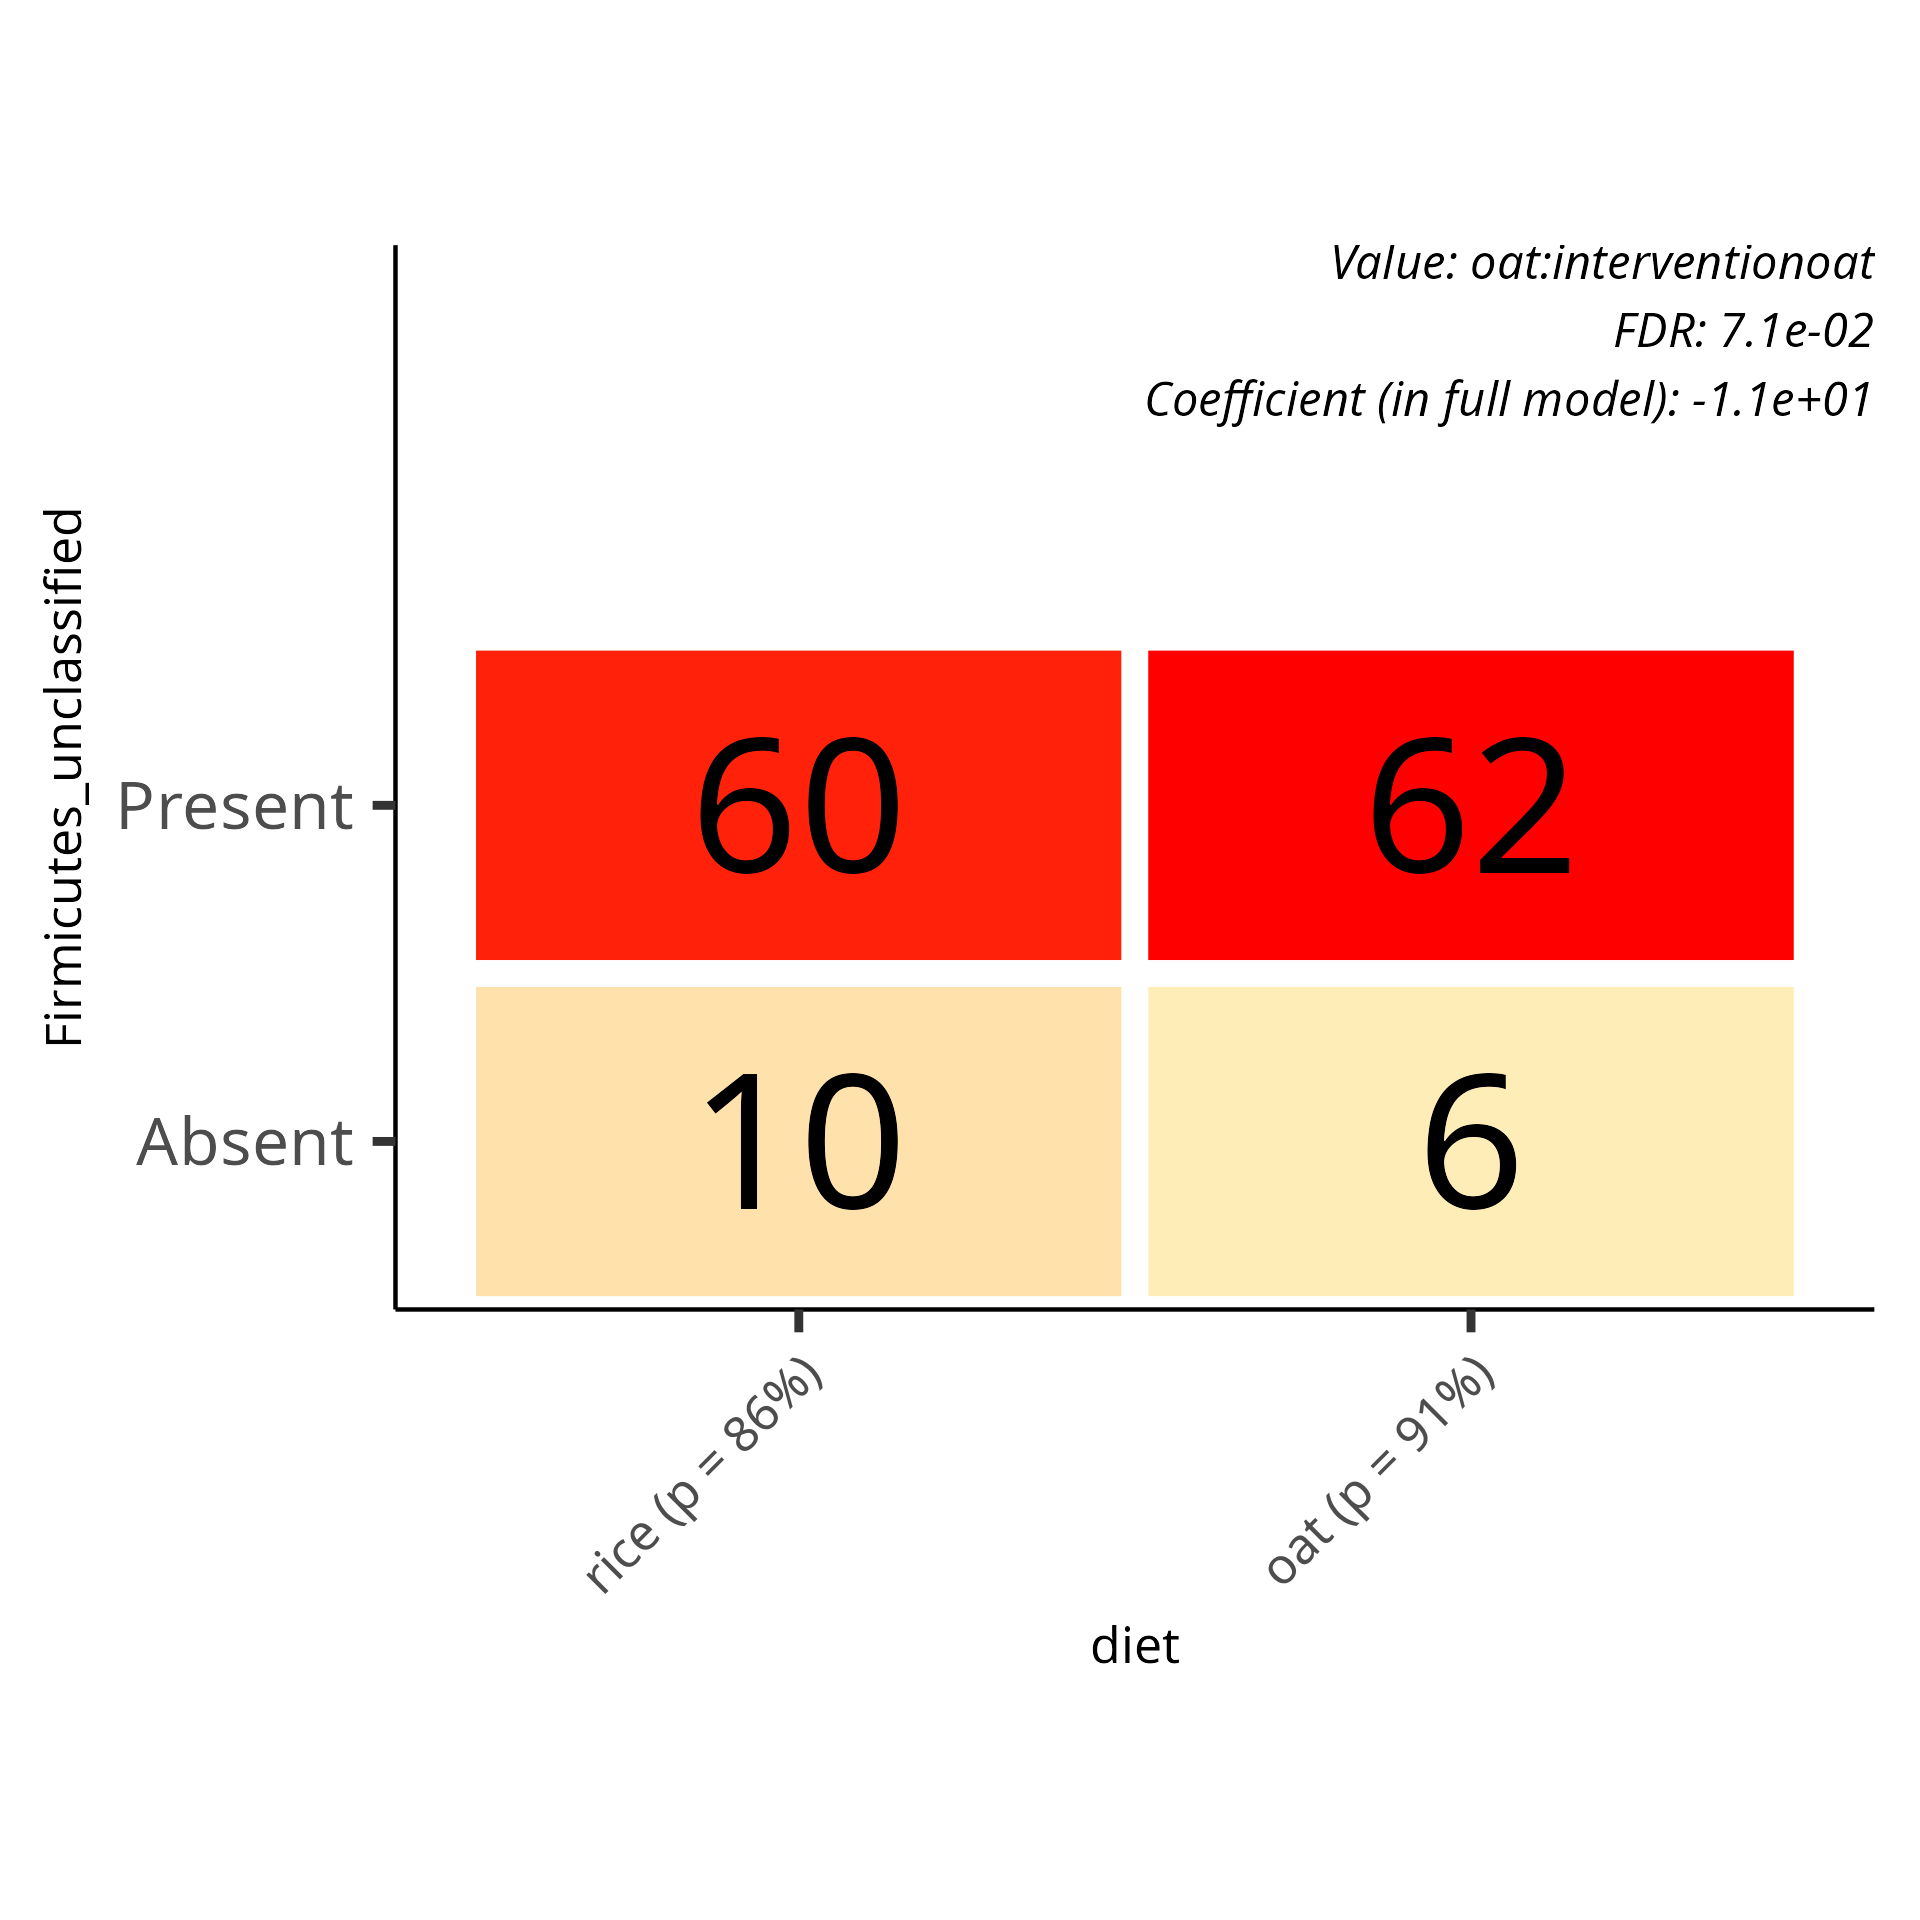
\includegraphics{../../output/daa/daa_taxa/family/figures/association_plots/diet/logistic/diet_Firmicutes_unclassified_logistic.png}\\
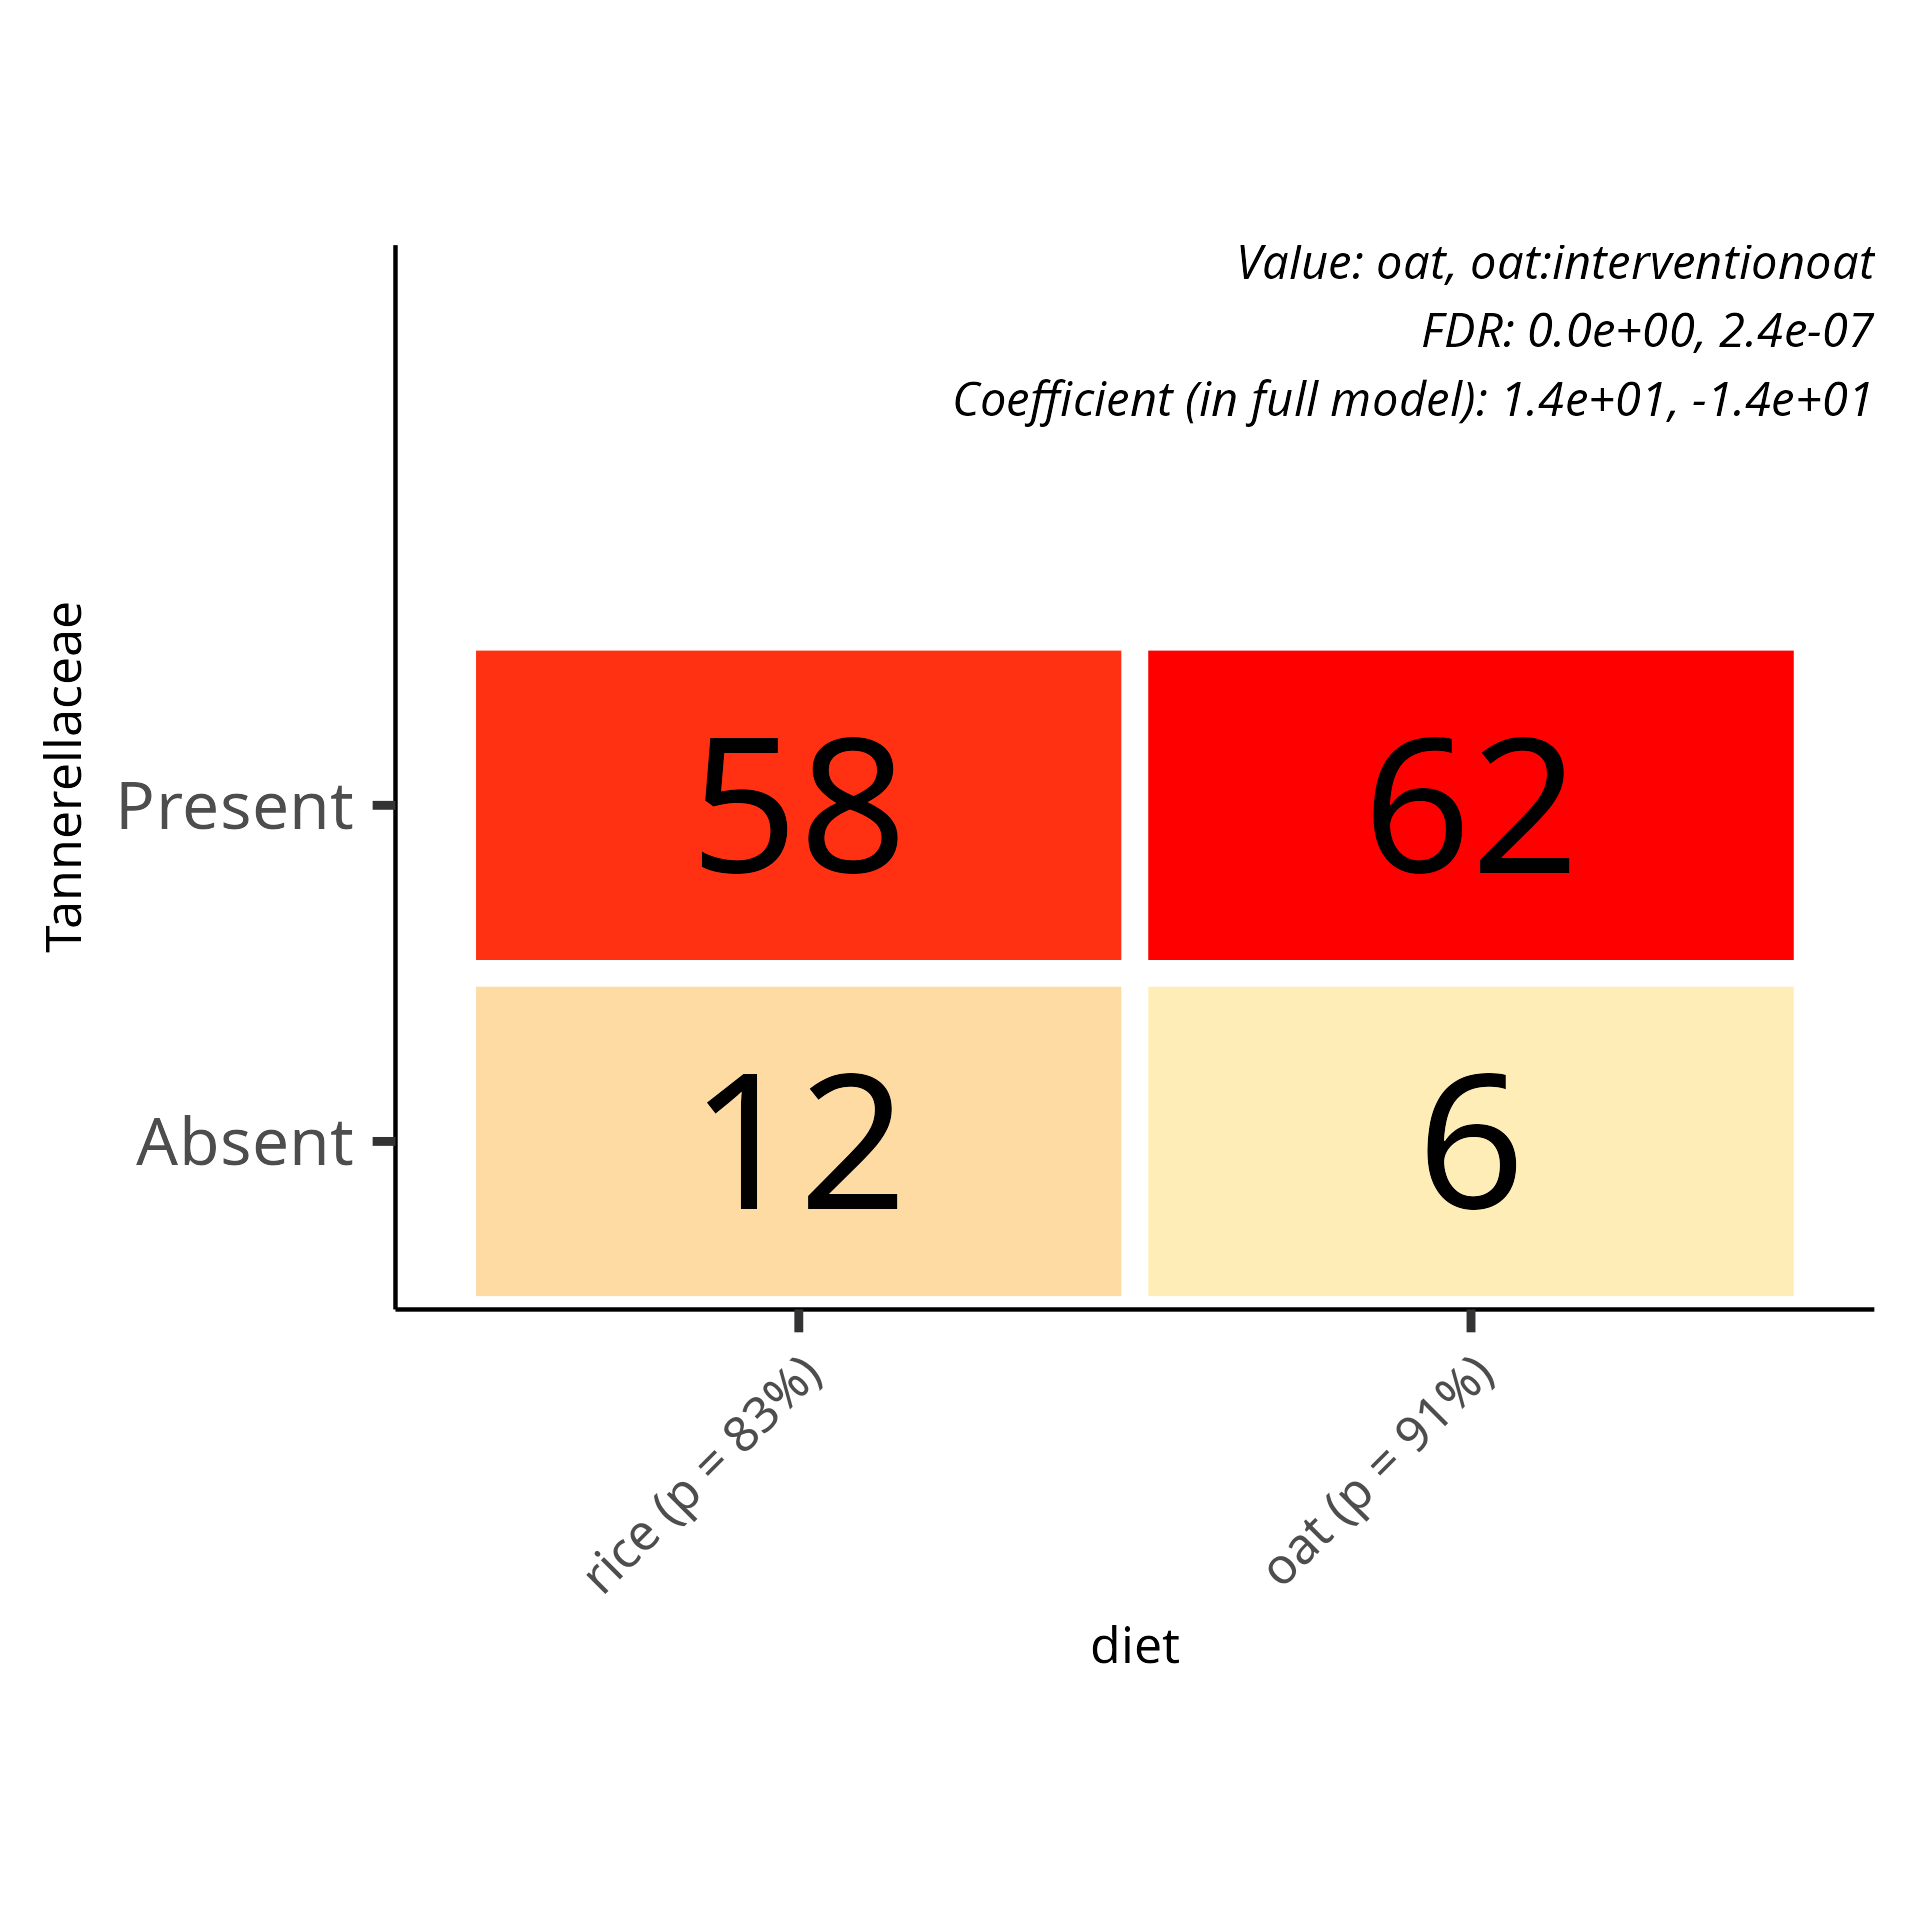
\includegraphics{../../output/daa/daa_taxa/family/figures/association_plots/diet/logistic/diet_Tannerellaceae_logistic.png}\\
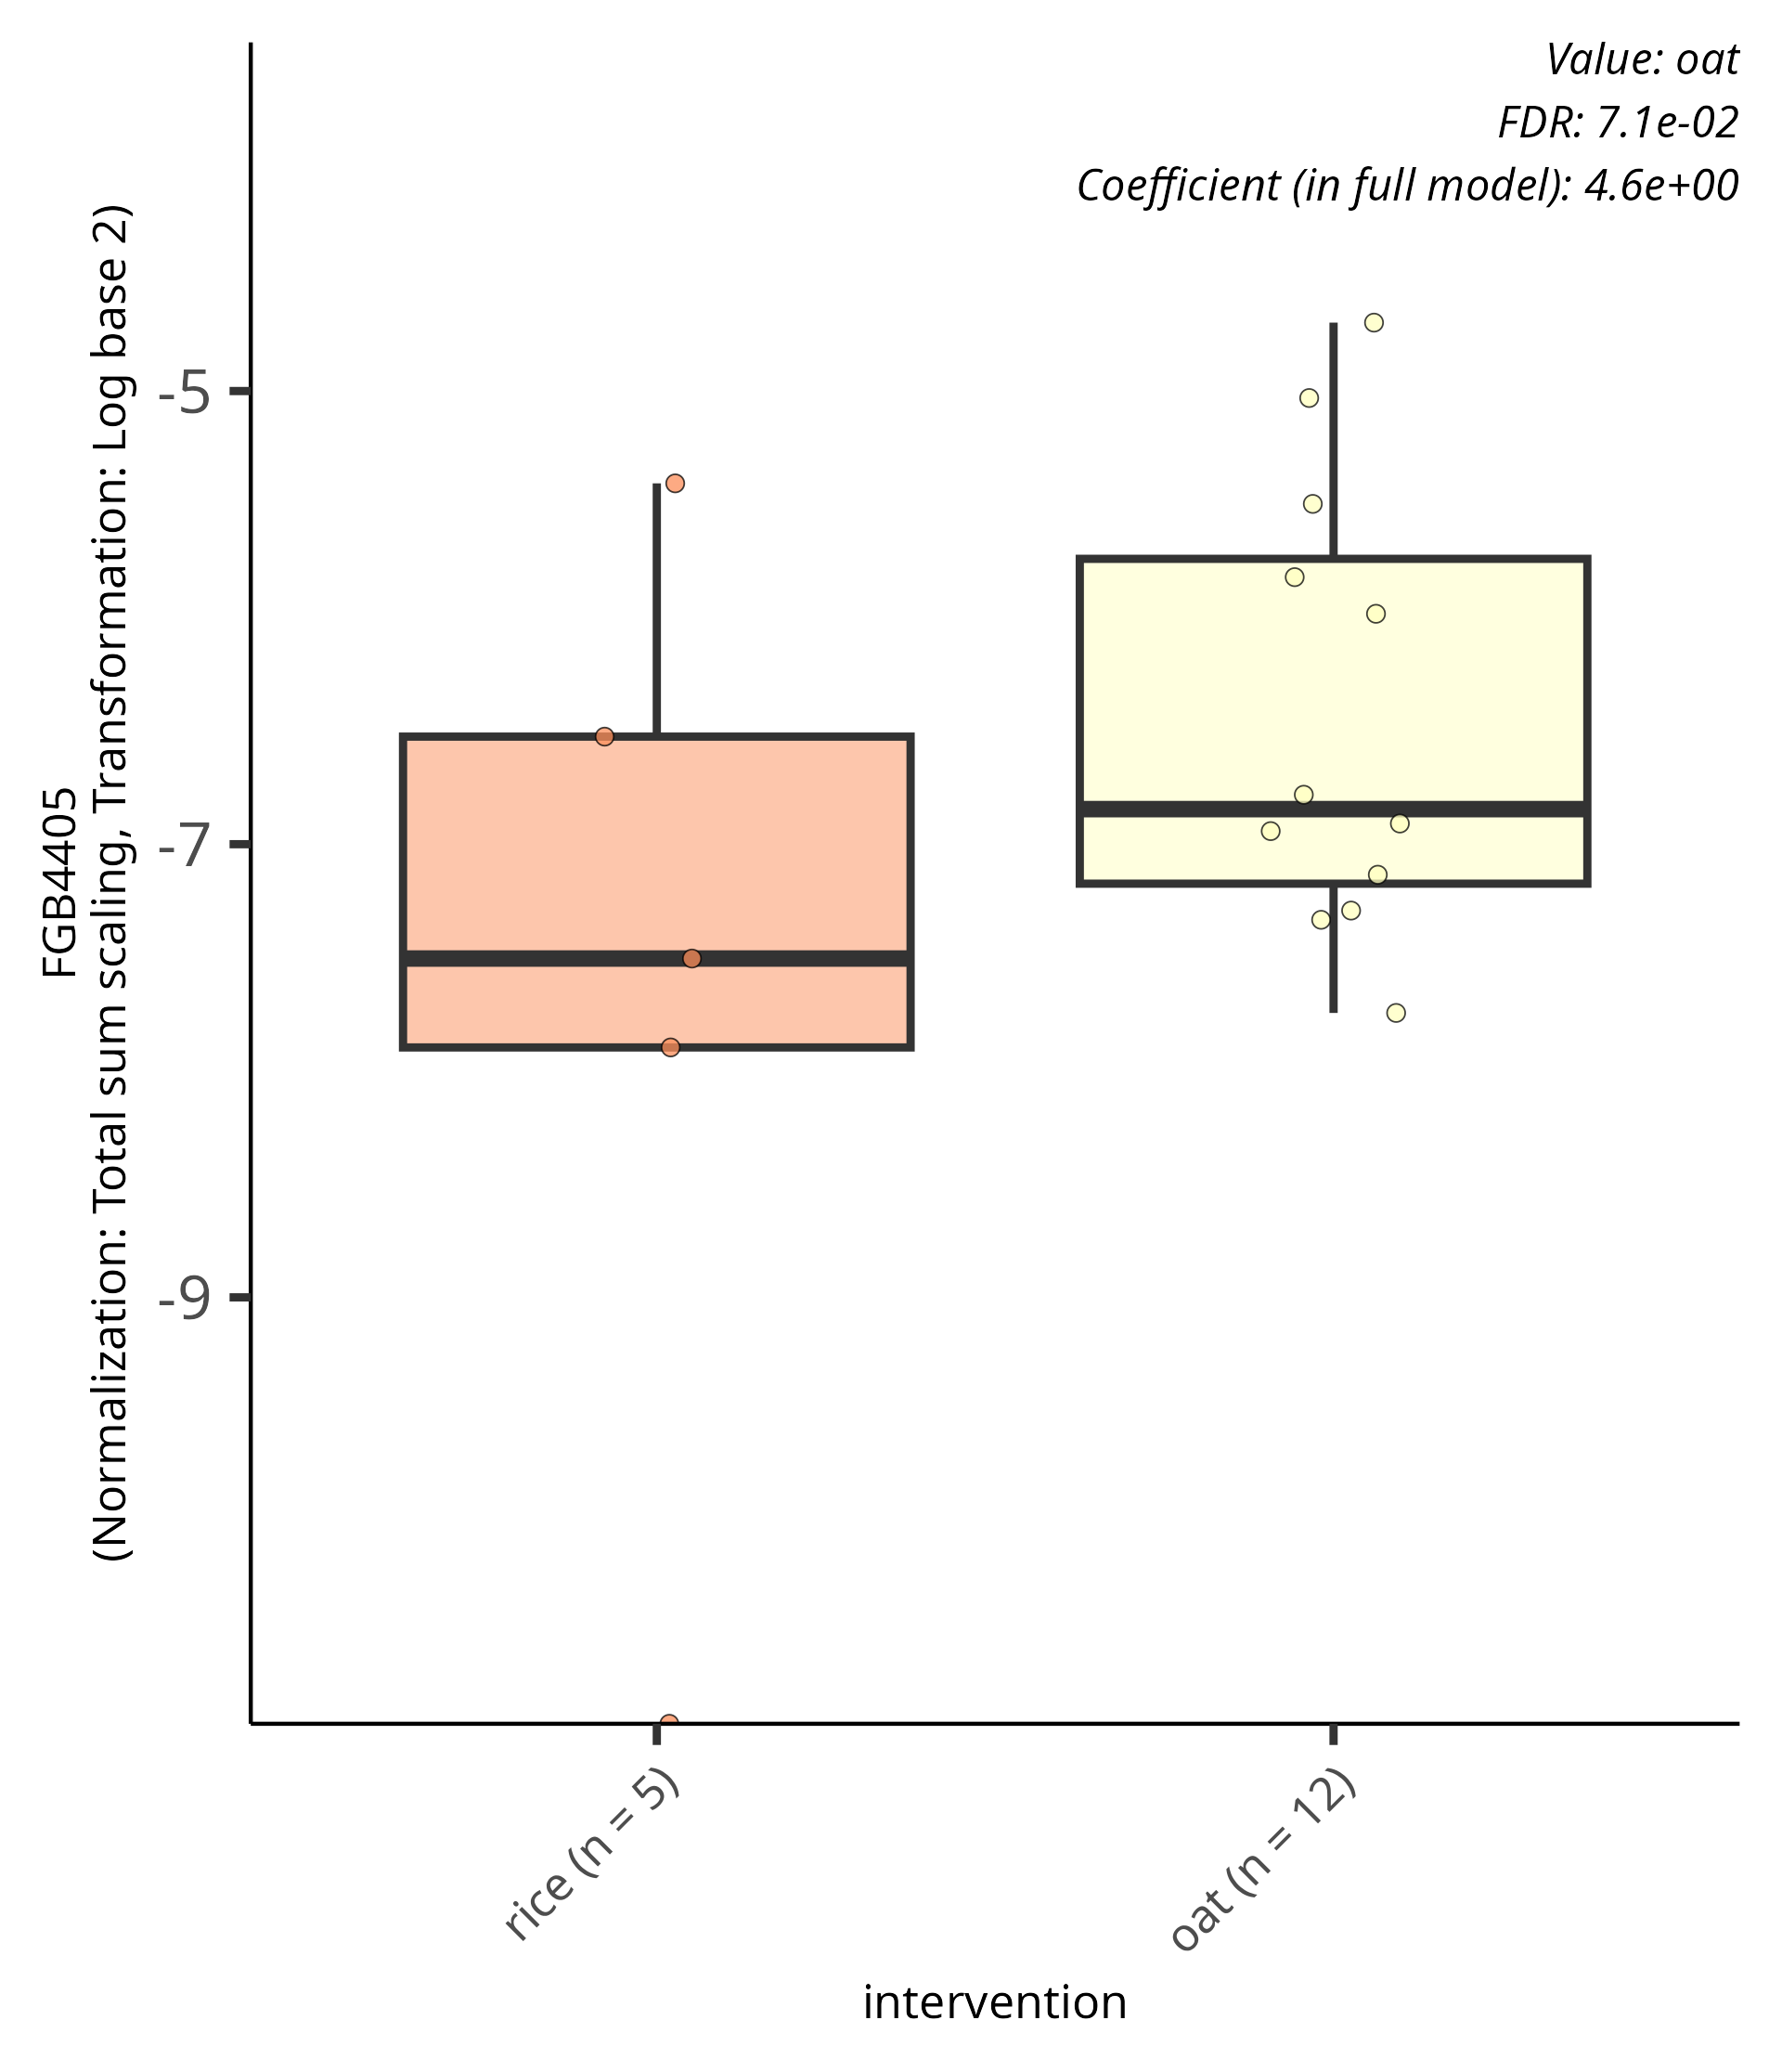
\includegraphics{../../output/daa/daa_taxa/family/figures/association_plots/intervention/linear/intervention_FGB4405_linear.png}\\
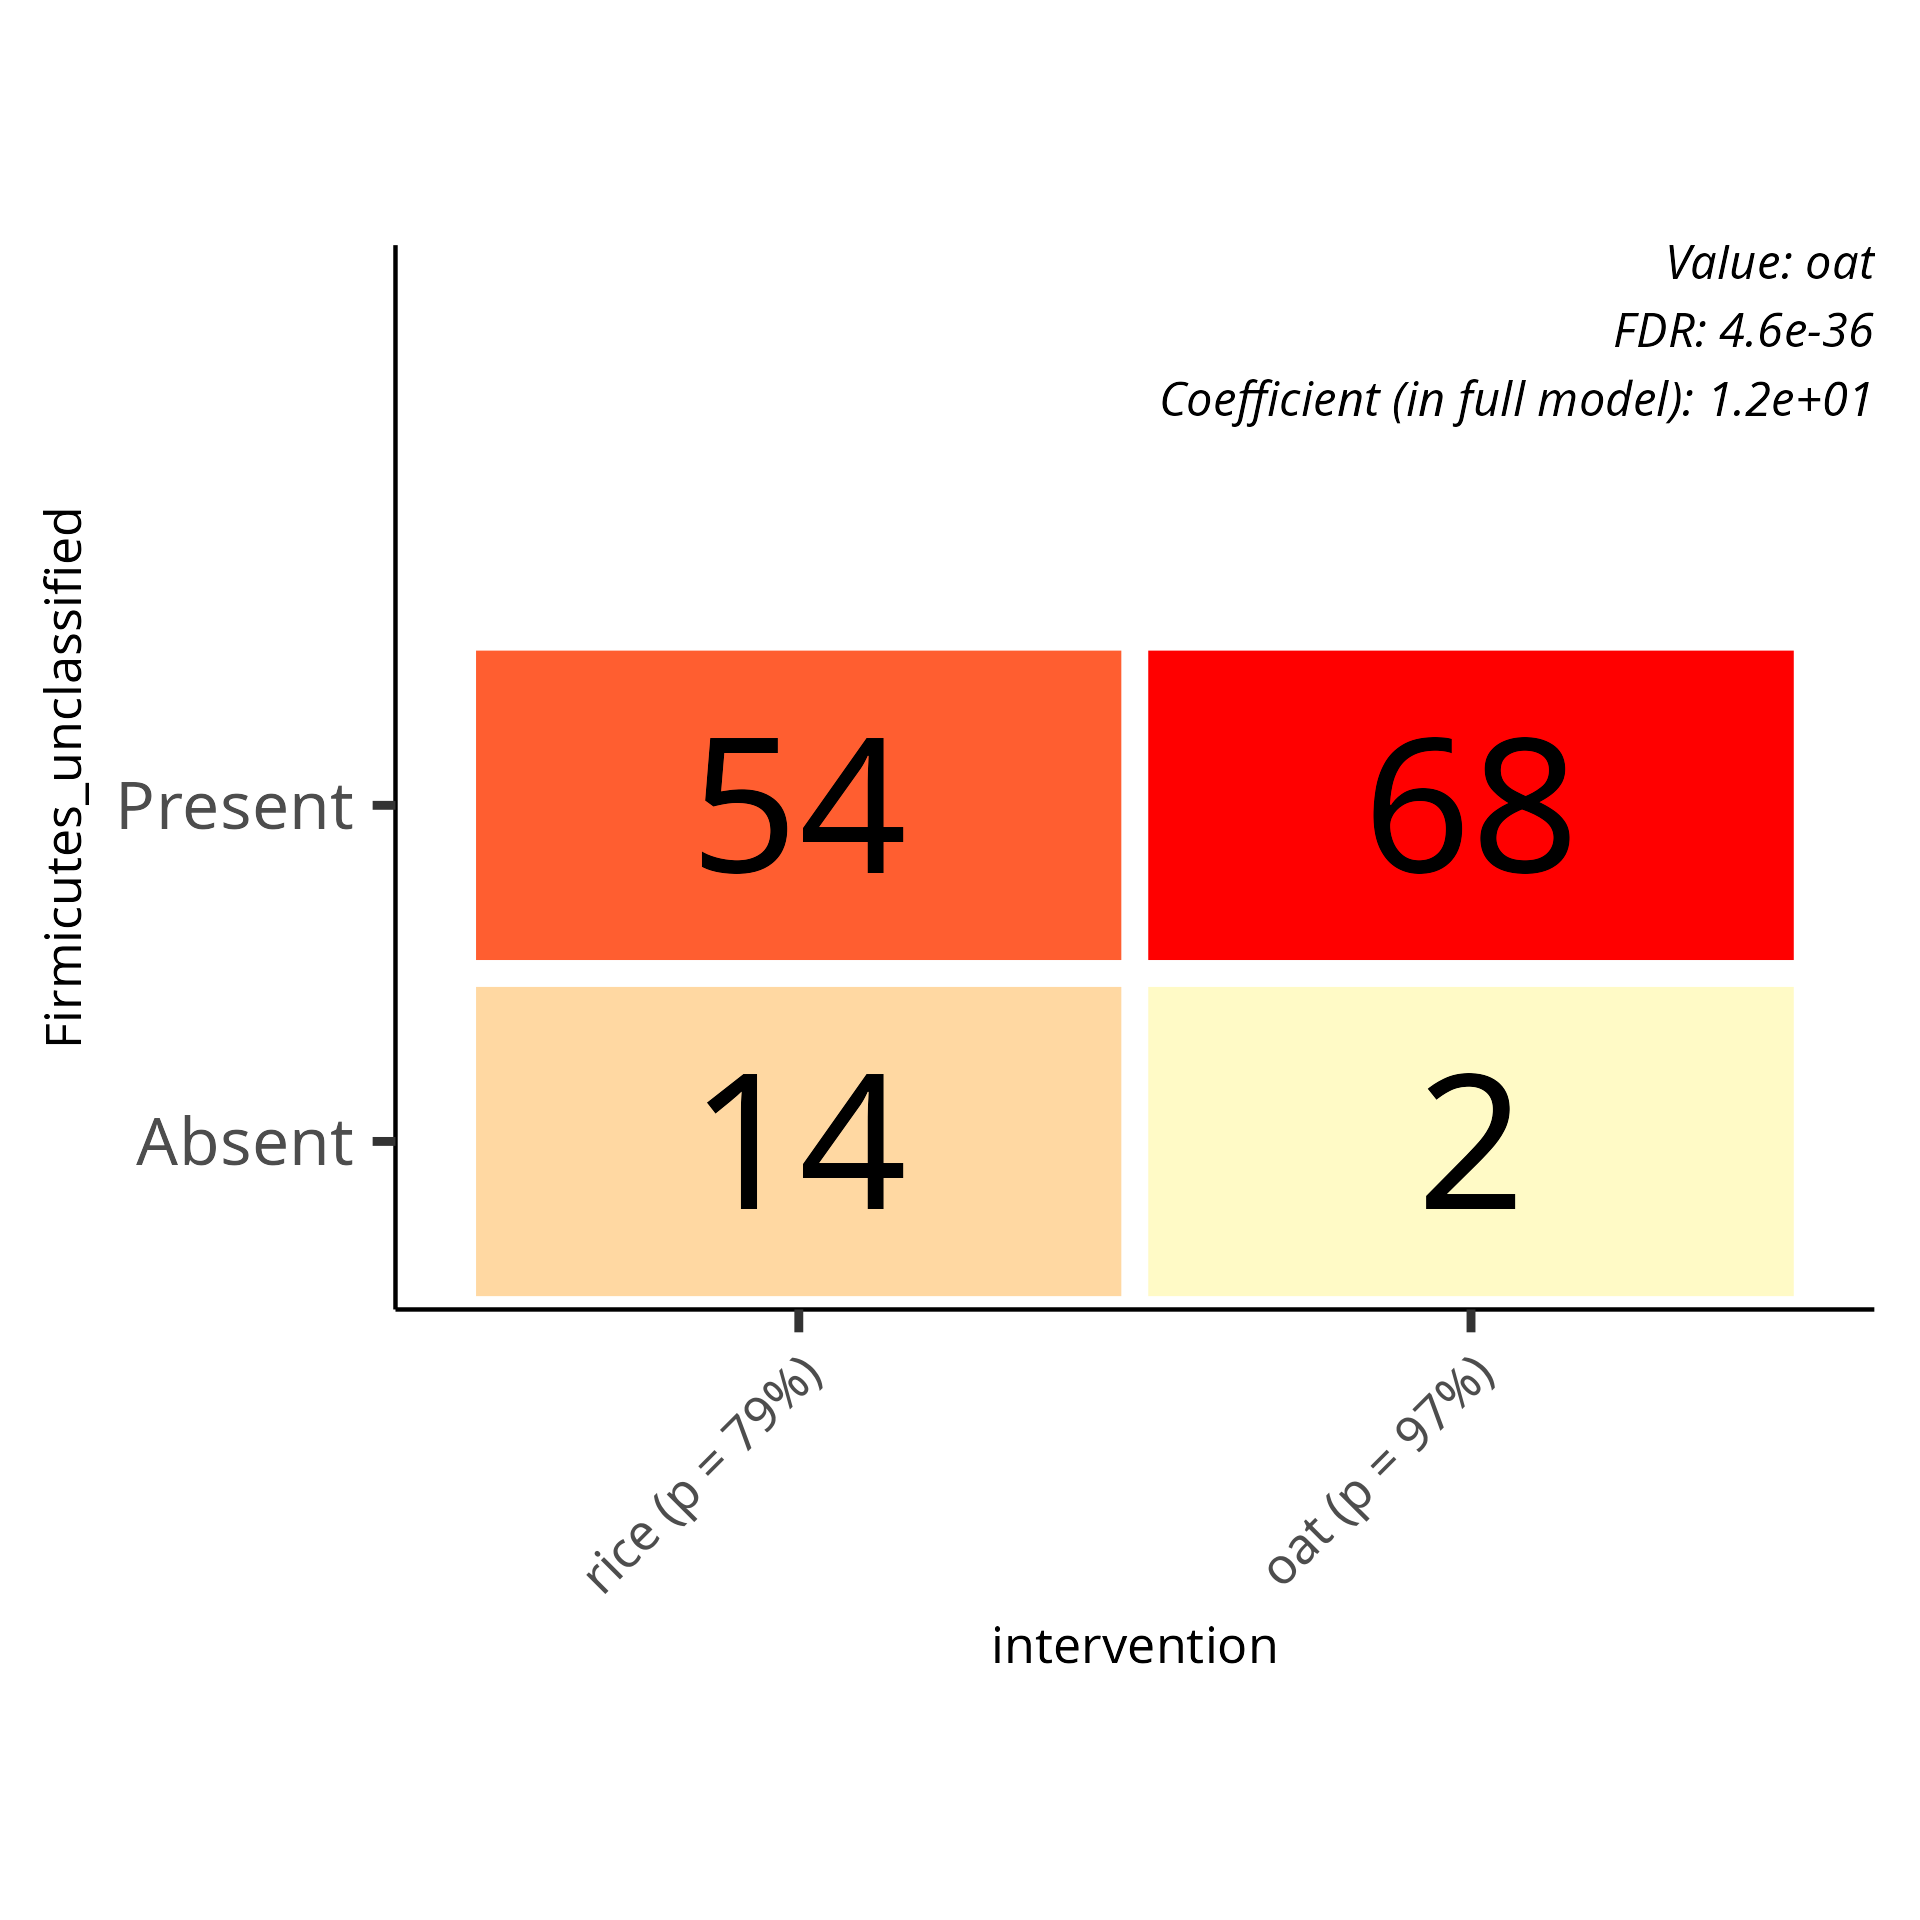
\includegraphics{../../output/daa/daa_taxa/family/figures/association_plots/intervention/logistic/intervention_Firmicutes_unclassified_logistic.png}

\subsubsection{Associations-genus}\label{associations-genus}

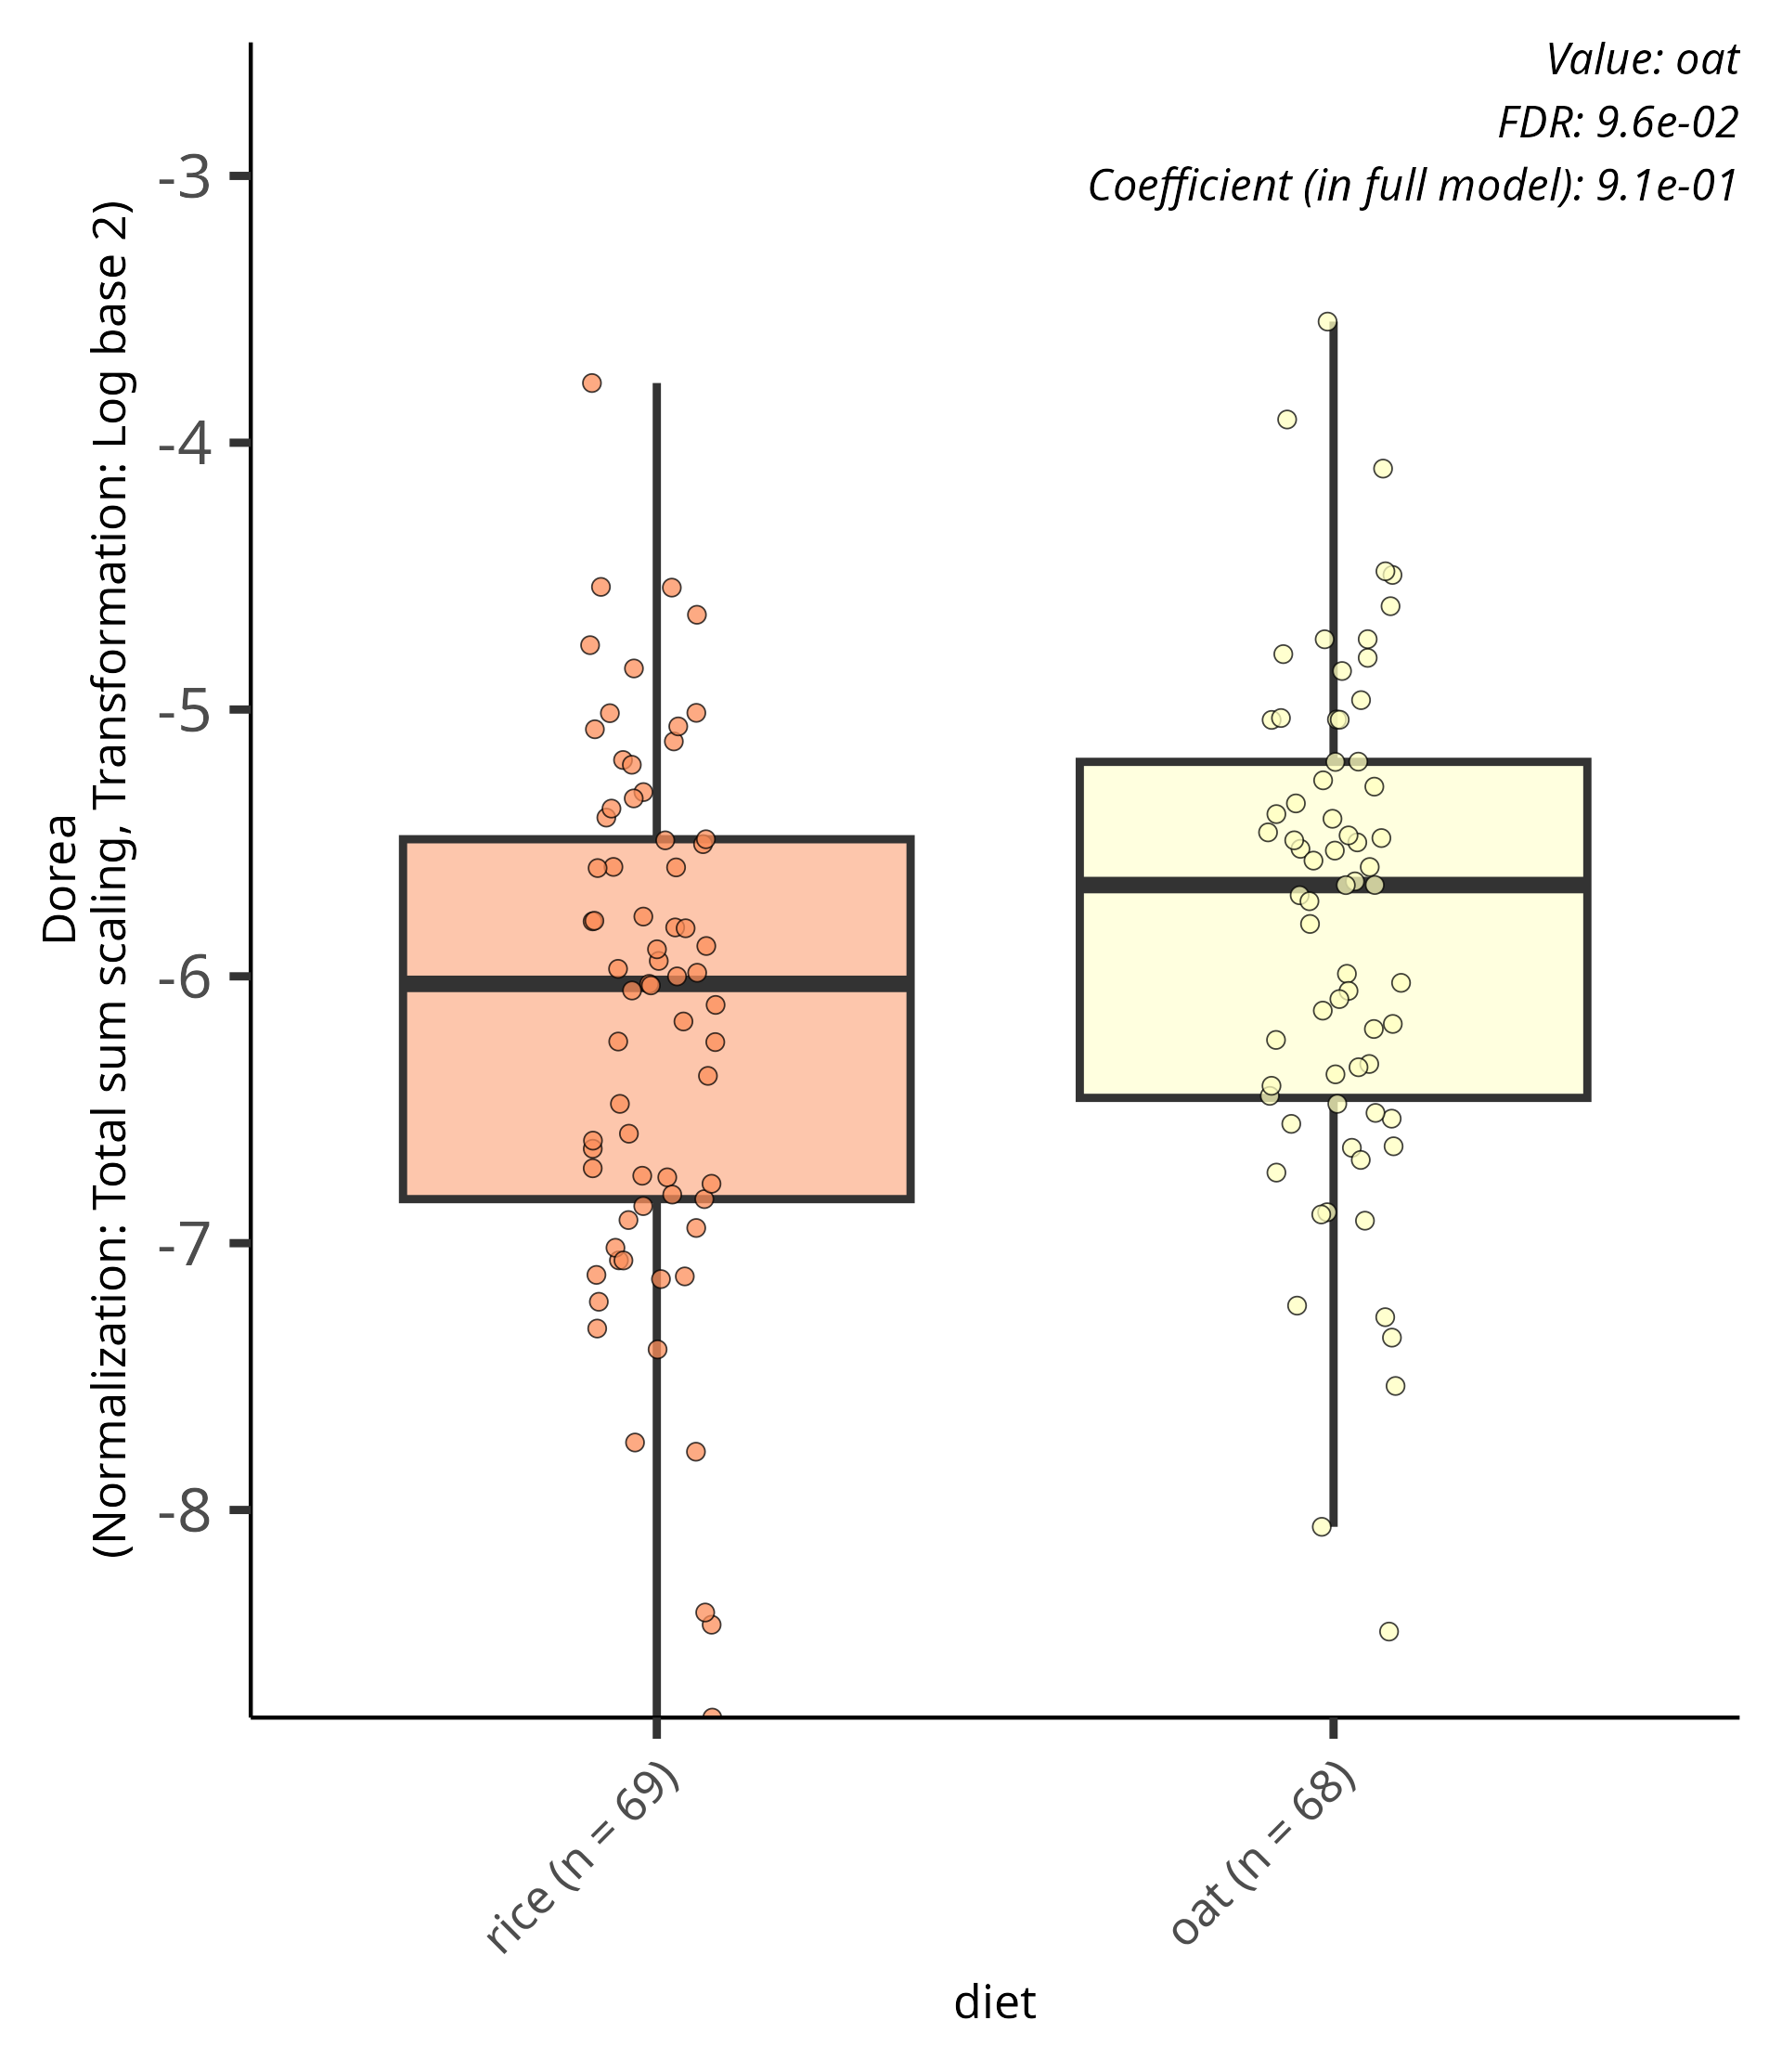
\includegraphics{../../output/daa/daa_taxa/genus/figures/association_plots/diet/linear/diet_Dorea_linear.png}\\
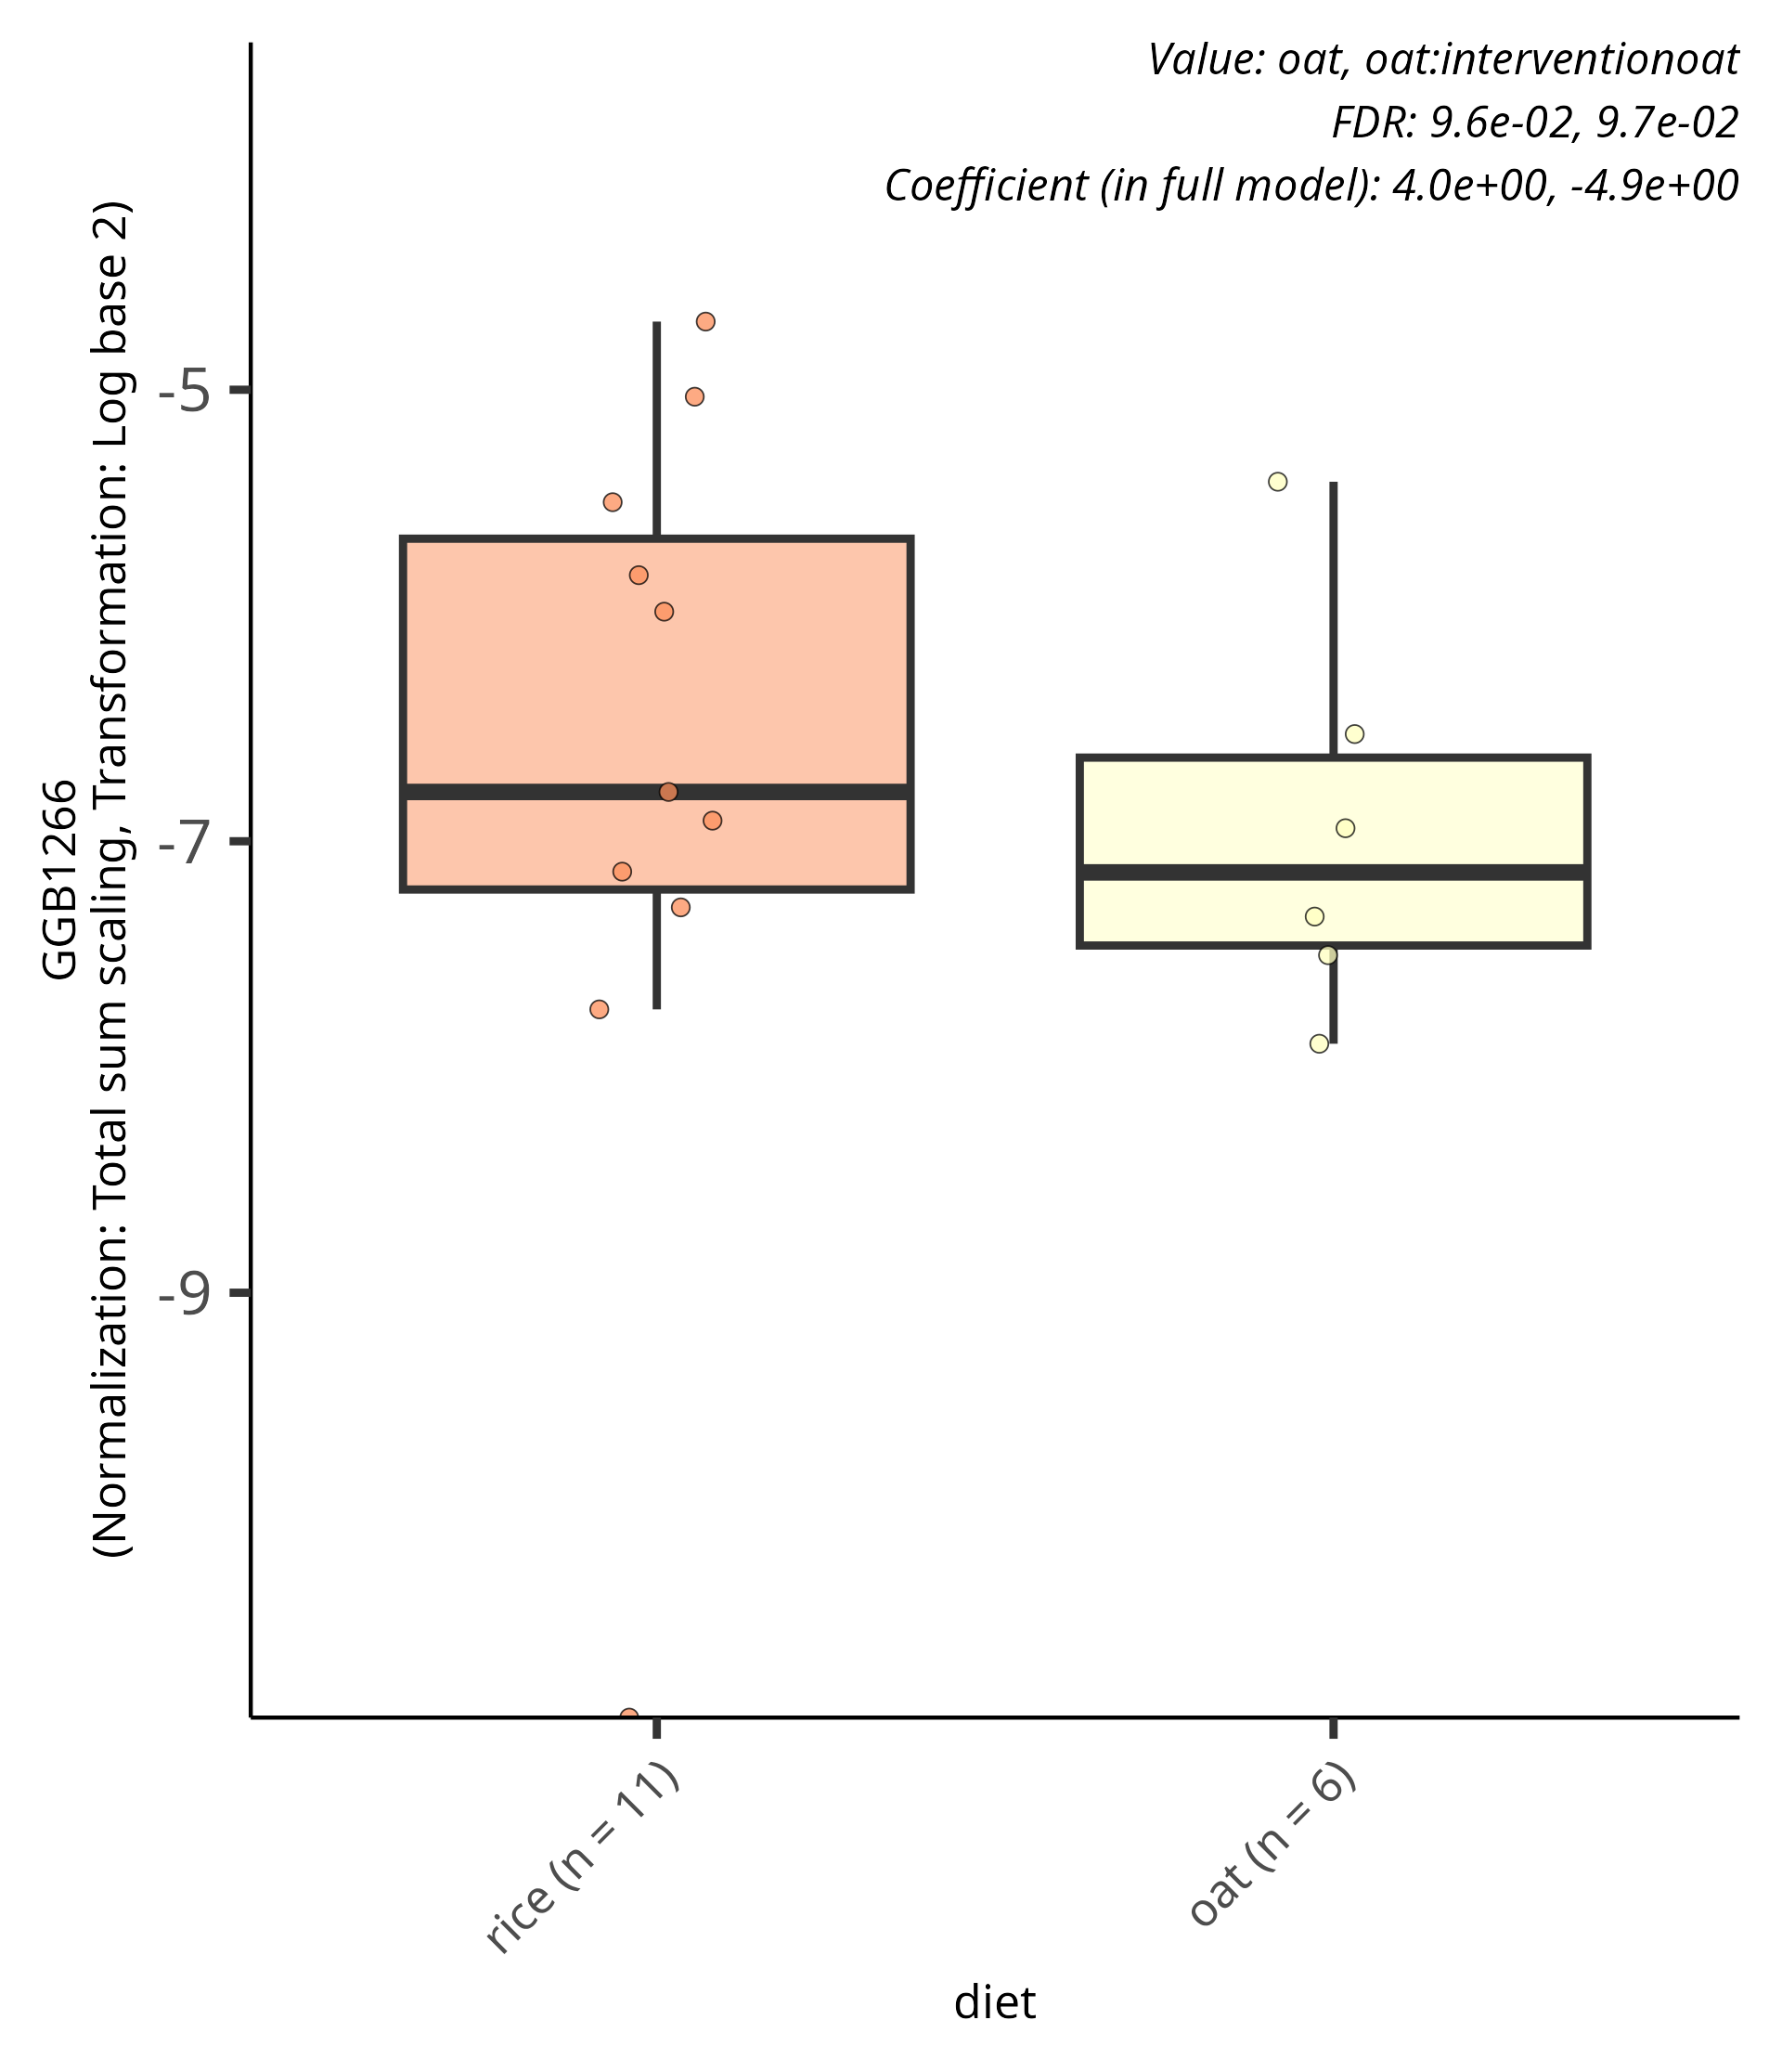
\includegraphics{../../output/daa/daa_taxa/genus/figures/association_plots/diet/linear/diet_GGB1266_linear.png}\\
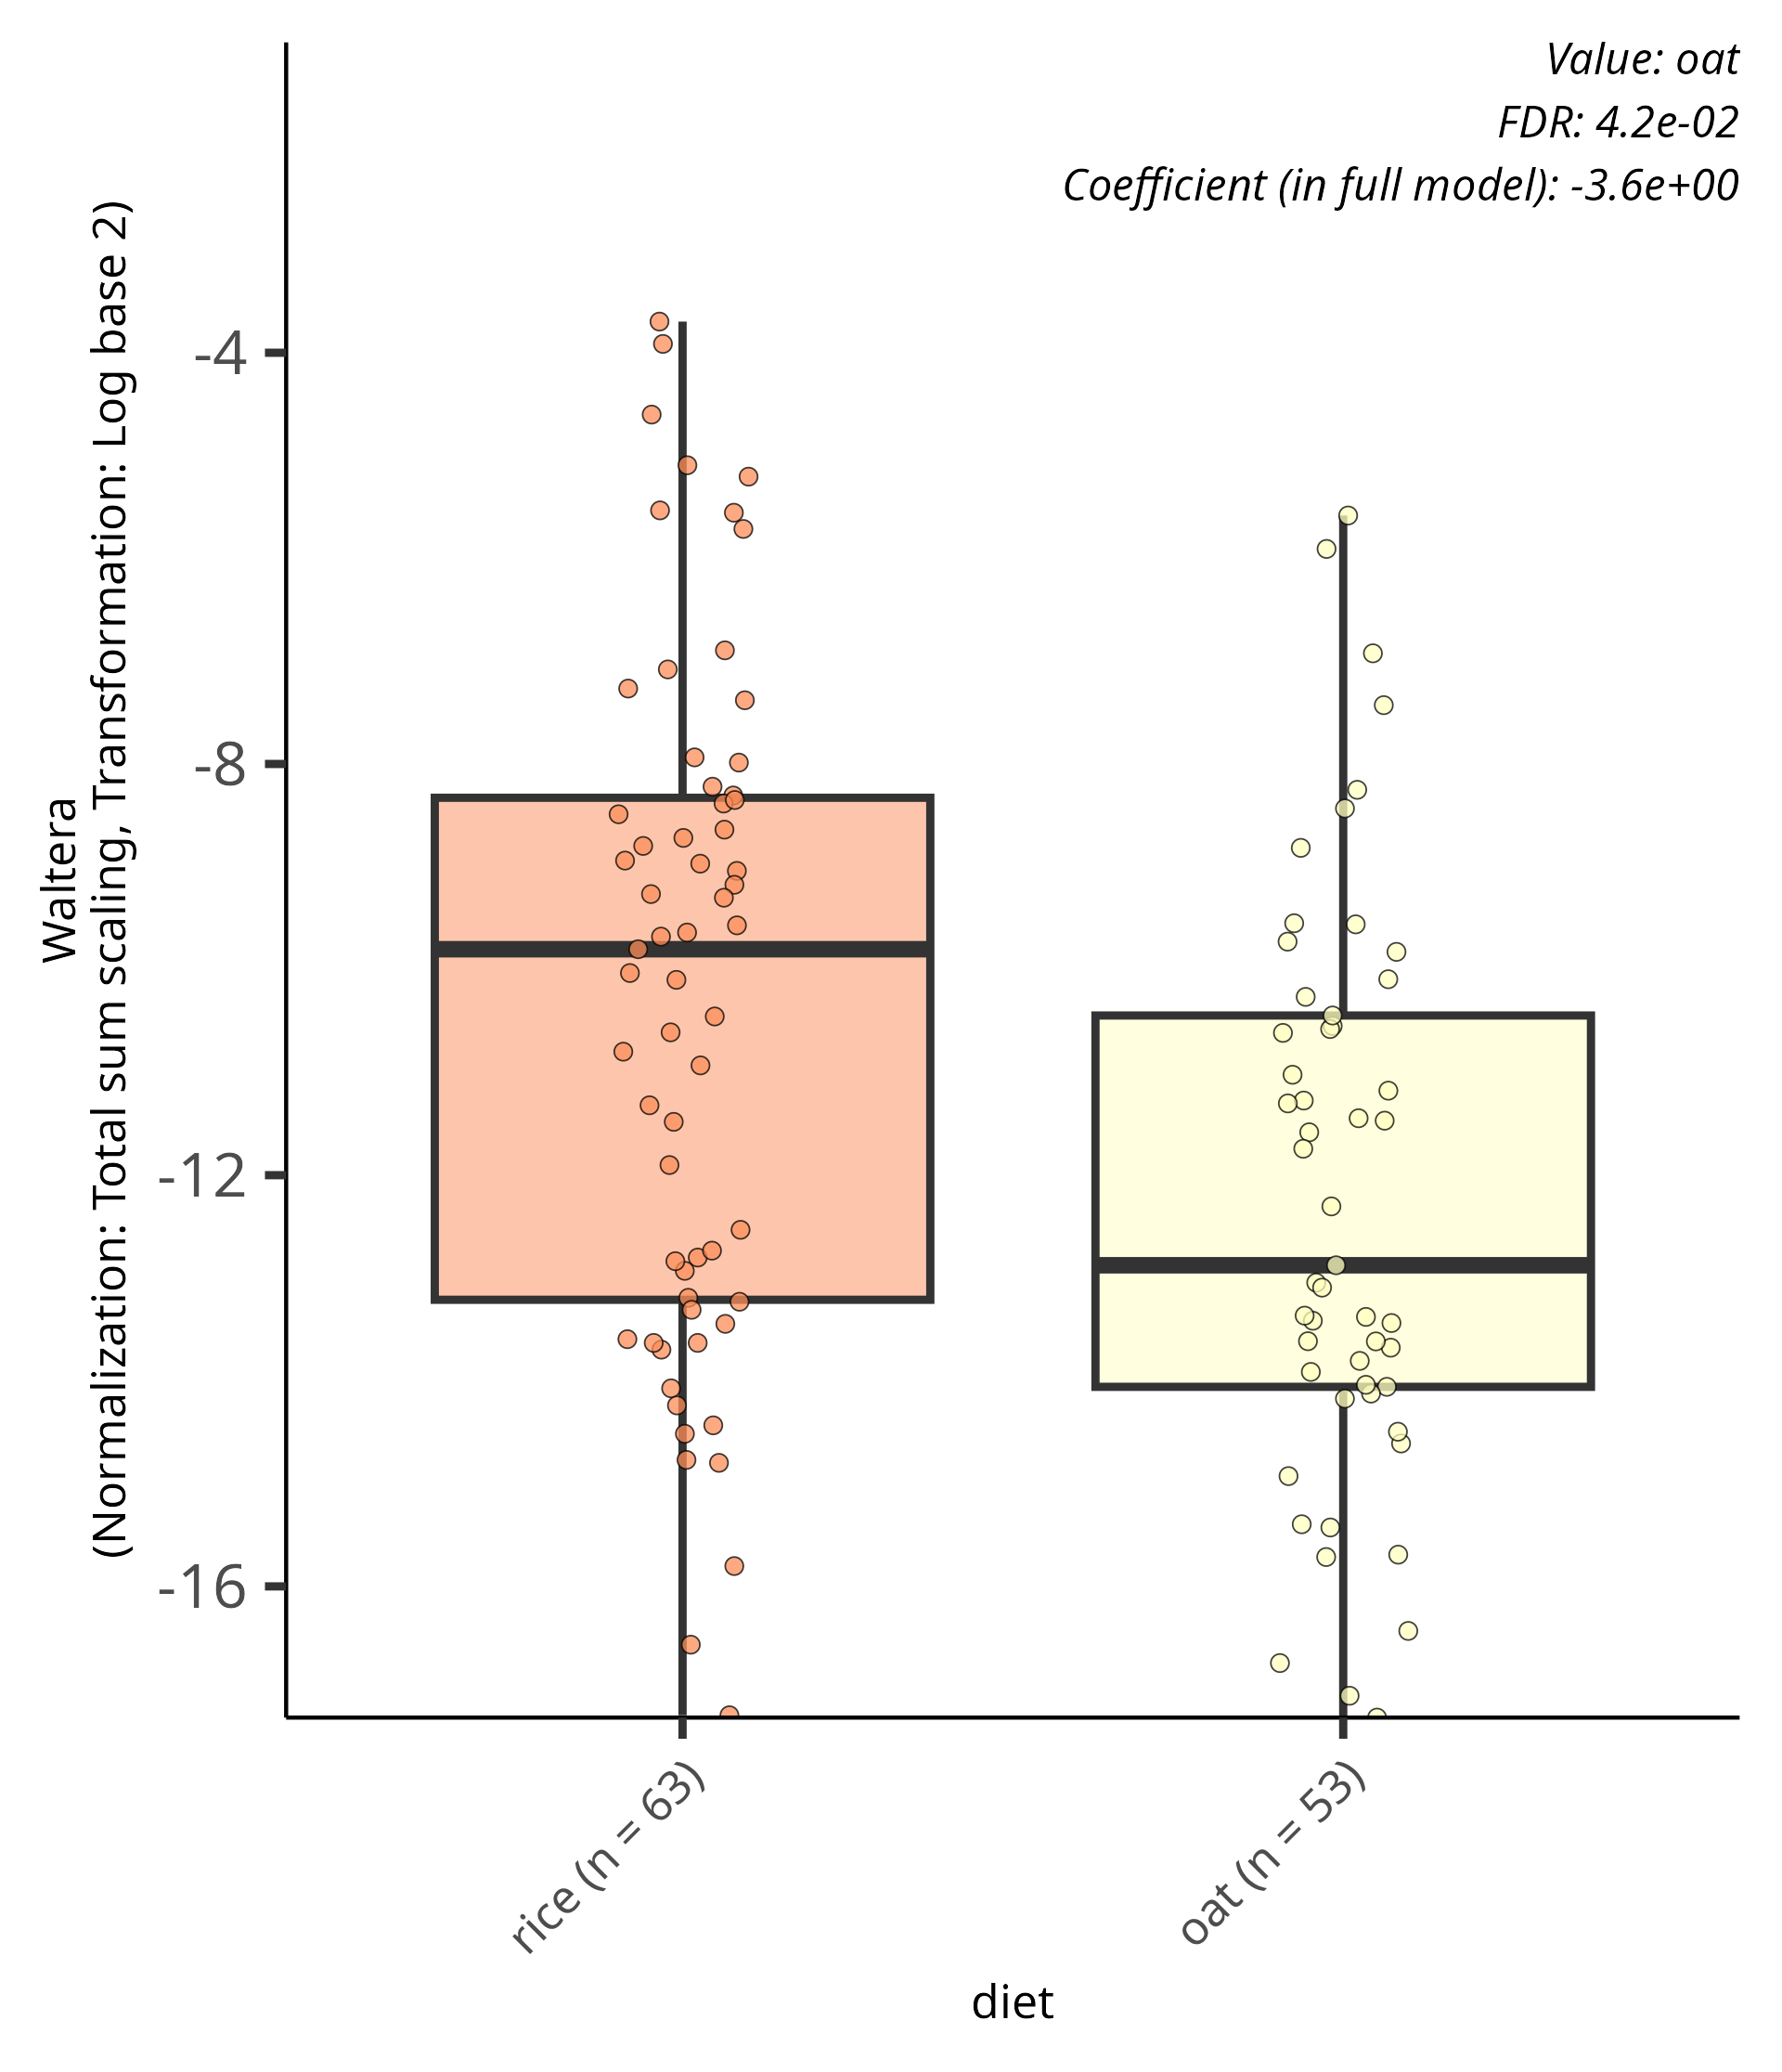
\includegraphics{../../output/daa/daa_taxa/genus/figures/association_plots/diet/linear/diet_Waltera_linear.png}\\
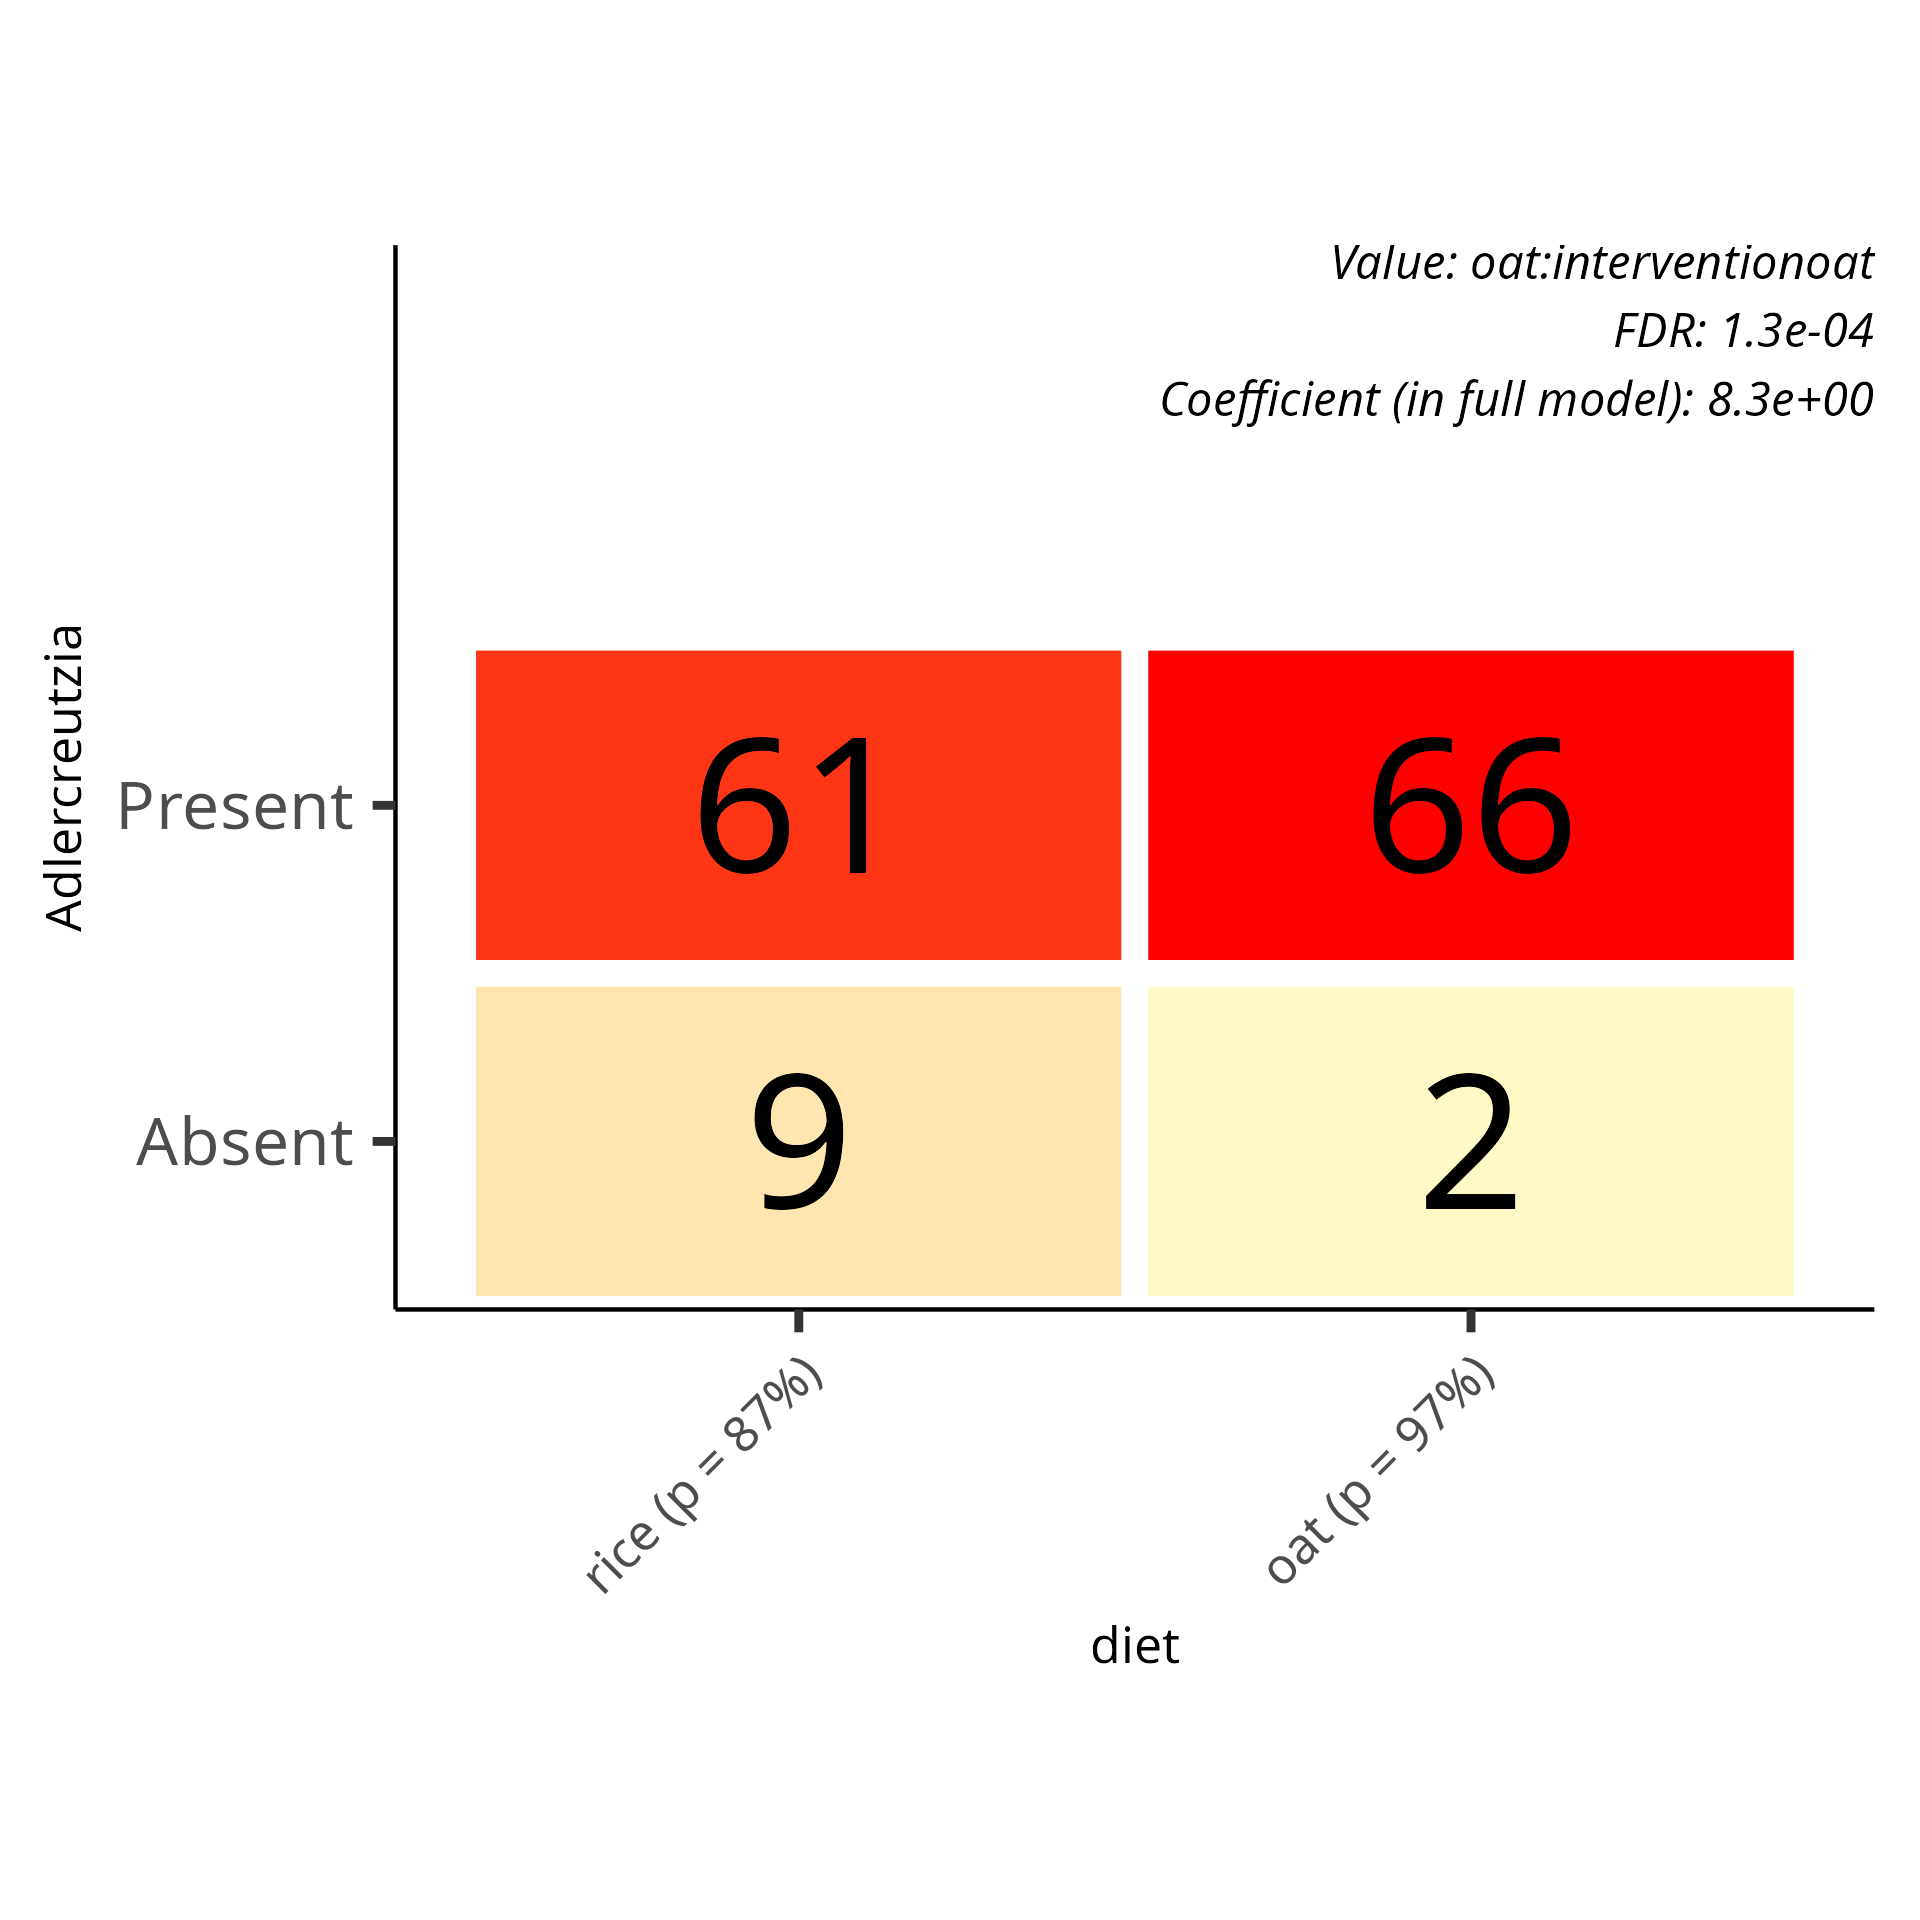
\includegraphics{../../output/daa/daa_taxa/genus/figures/association_plots/diet/logistic/diet_Adlercreutzia_logistic.png}\\
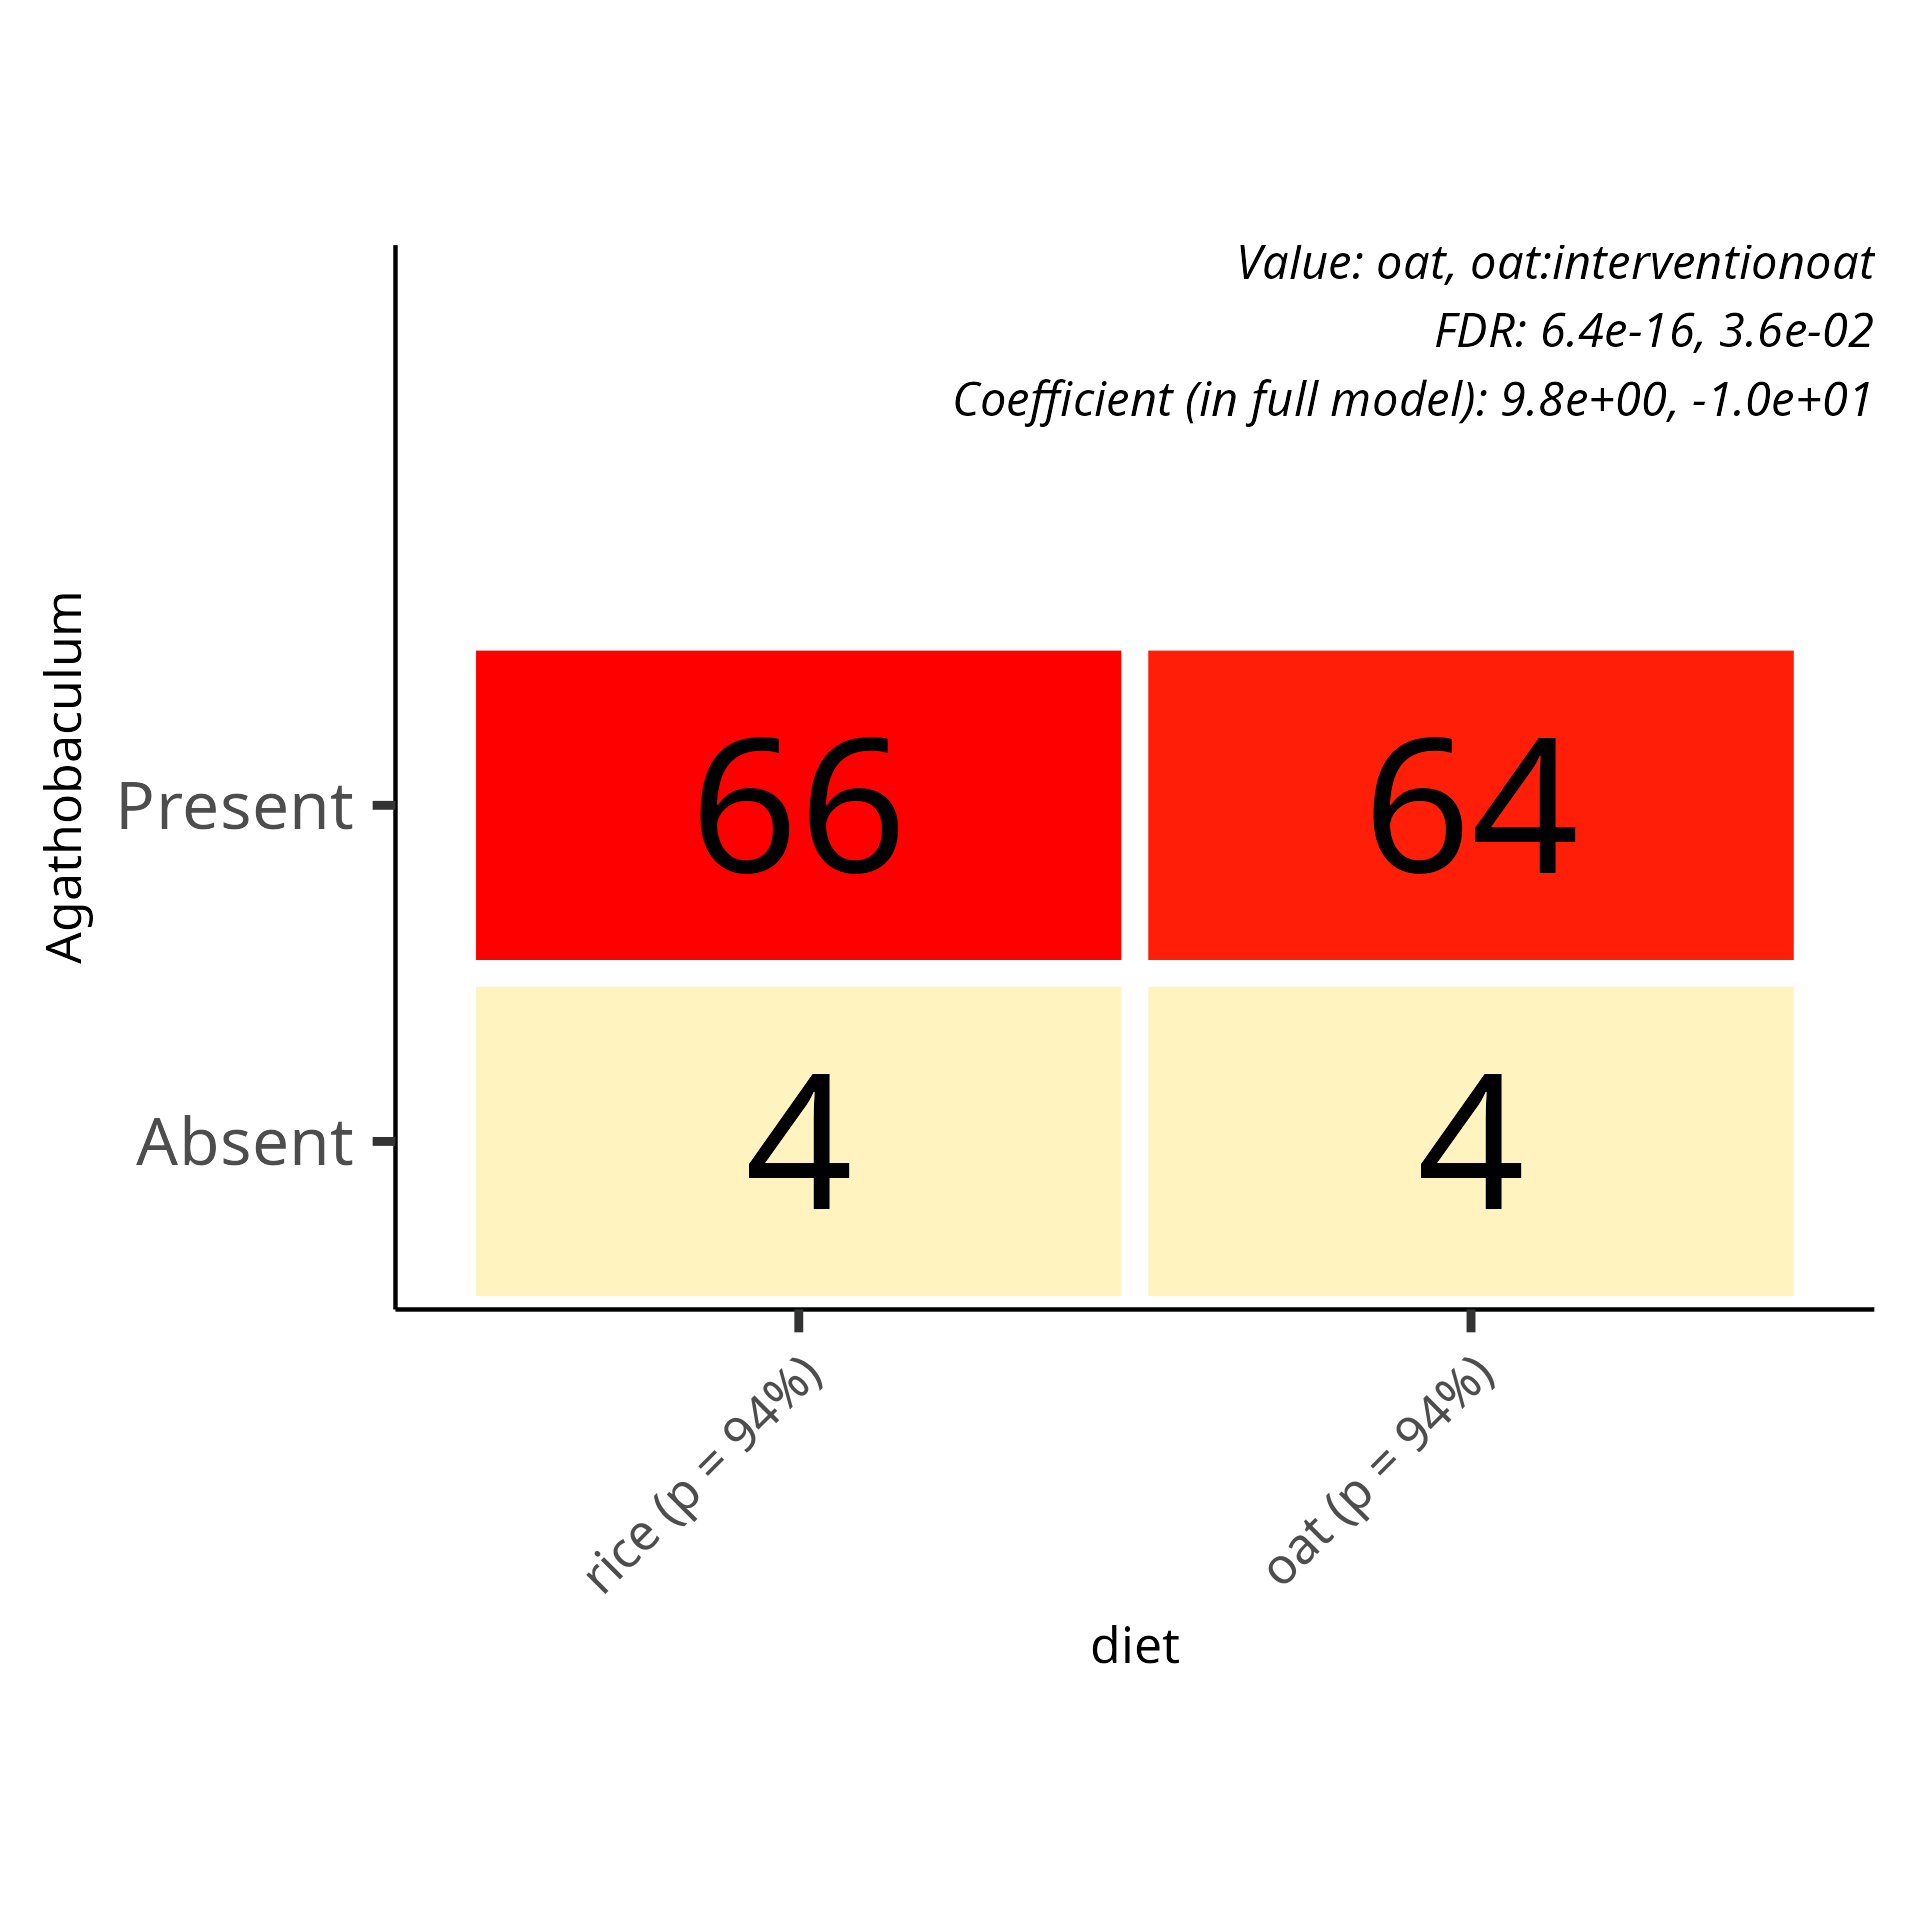
\includegraphics{../../output/daa/daa_taxa/genus/figures/association_plots/diet/logistic/diet_Agathobaculum_logistic.png}\\
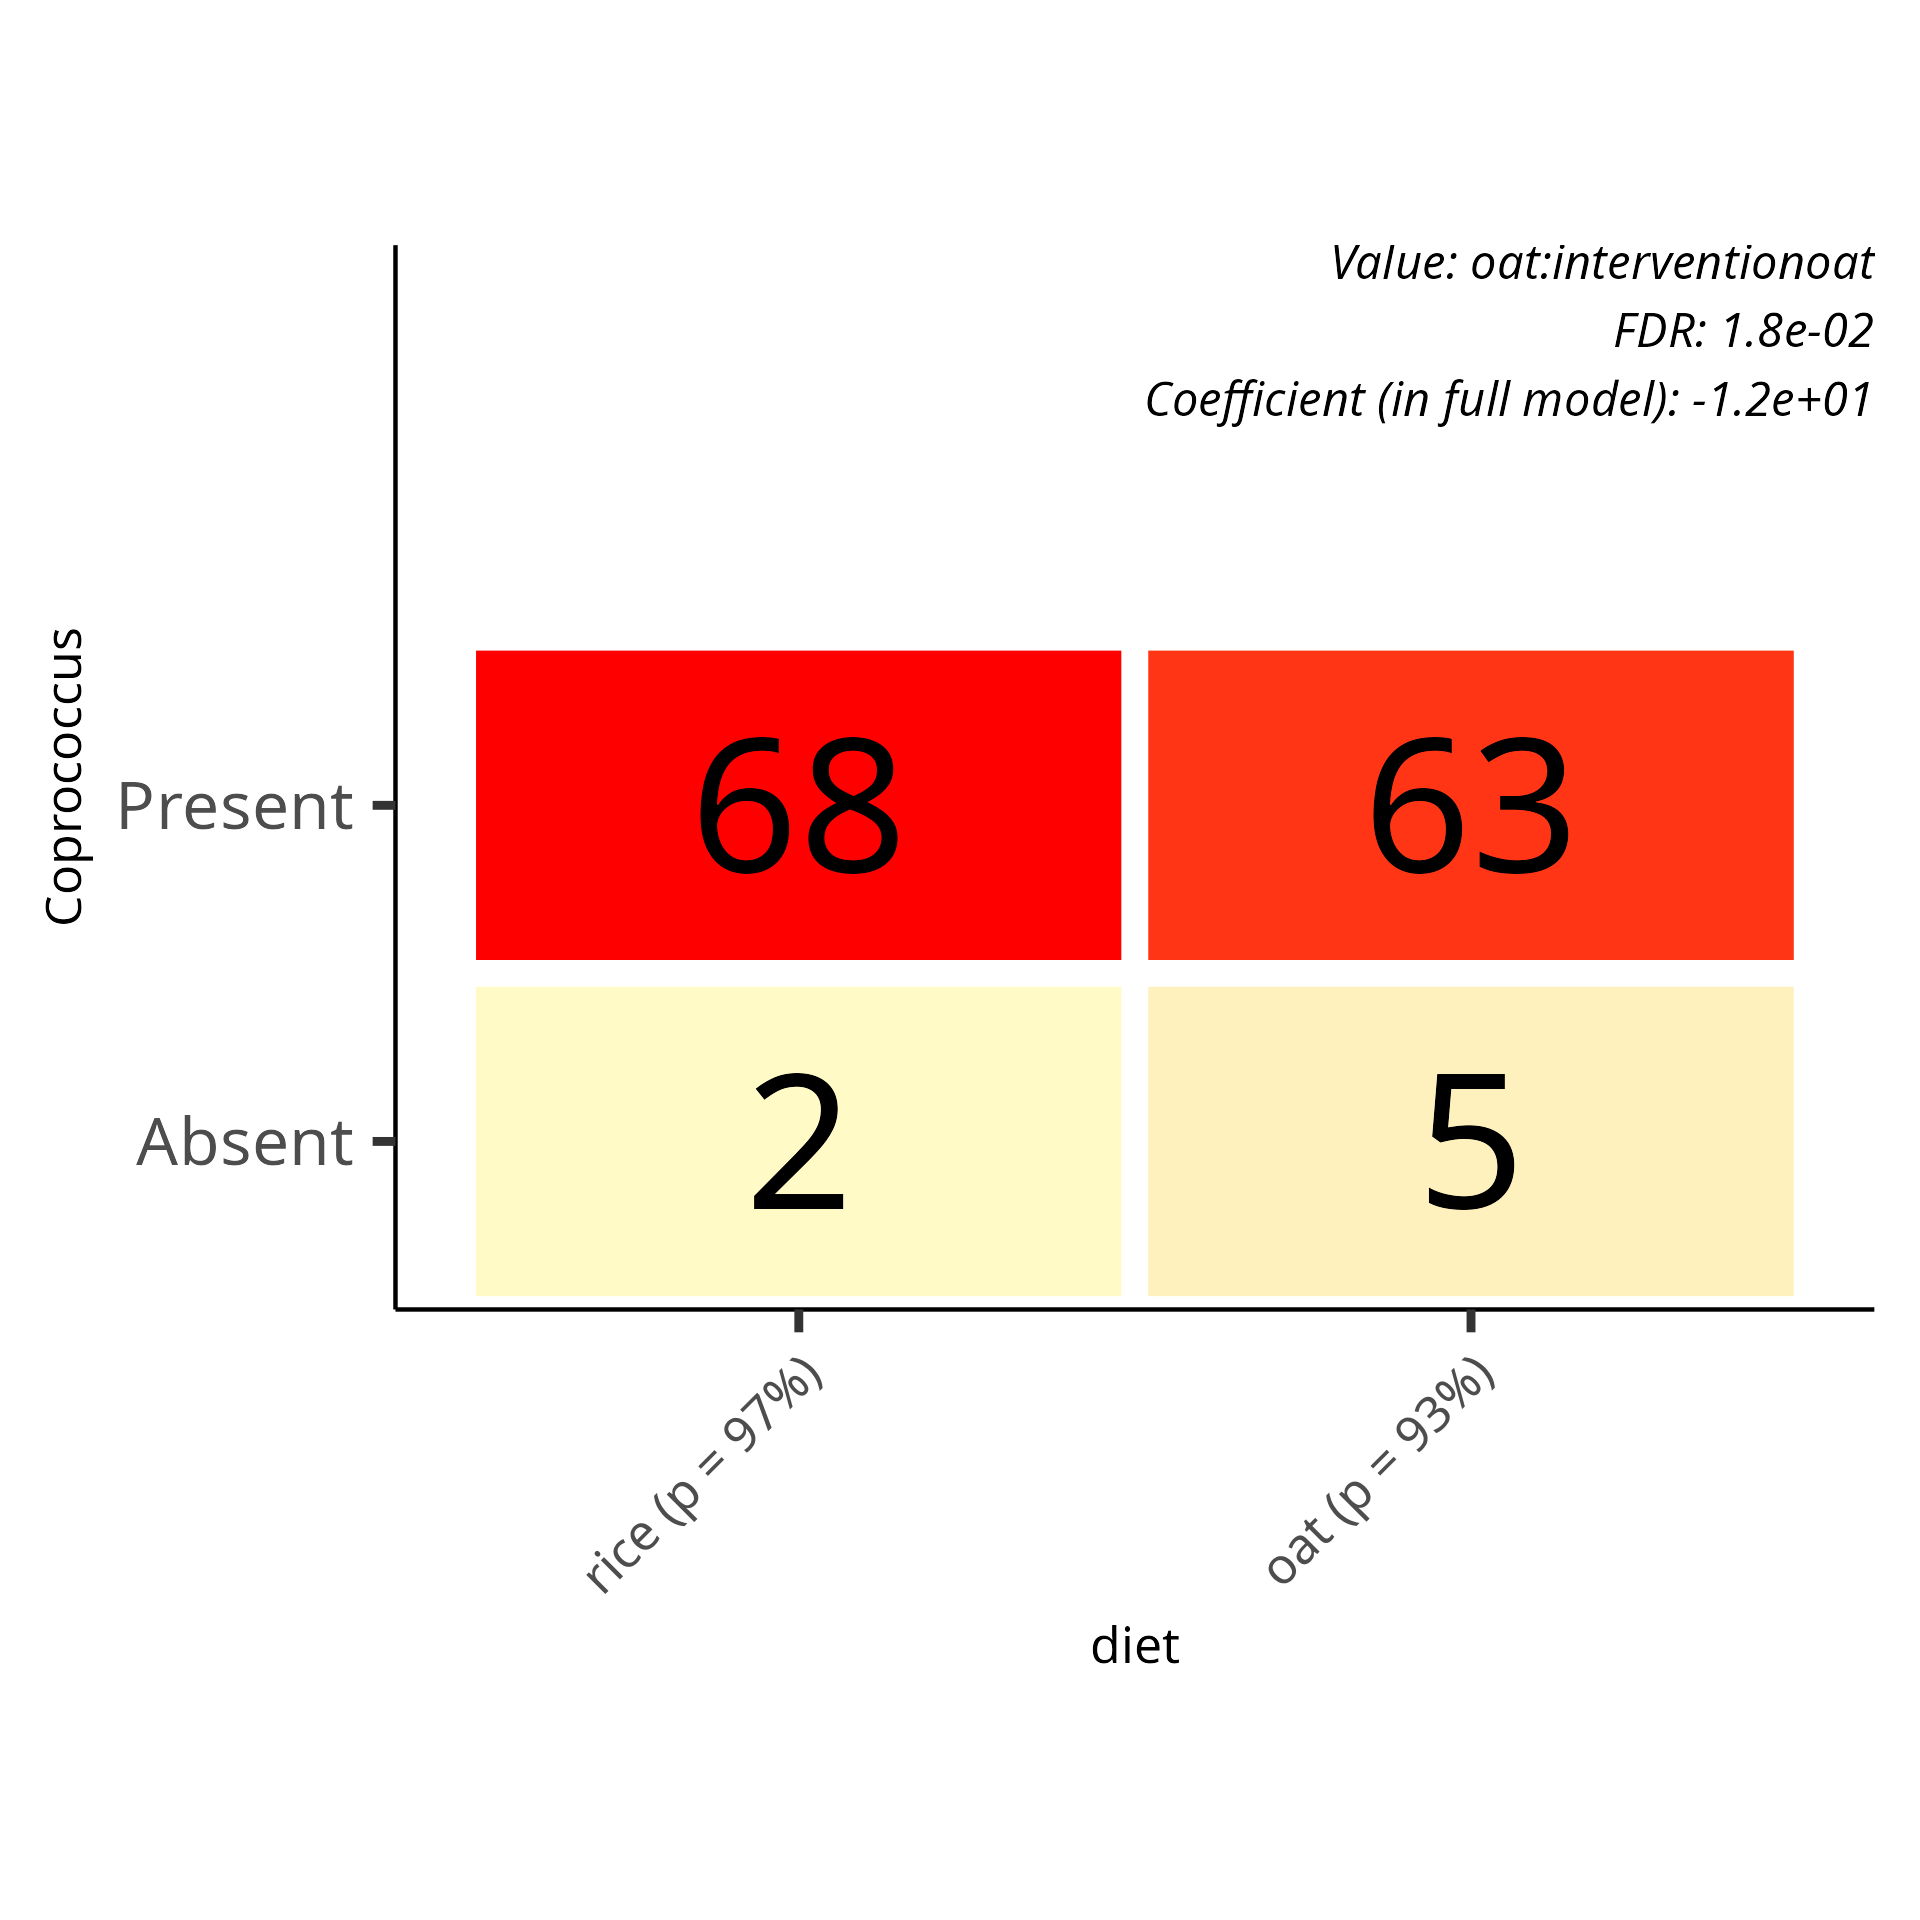
\includegraphics{../../output/daa/daa_taxa/genus/figures/association_plots/diet/logistic/diet_Coprococcus_logistic.png}\\
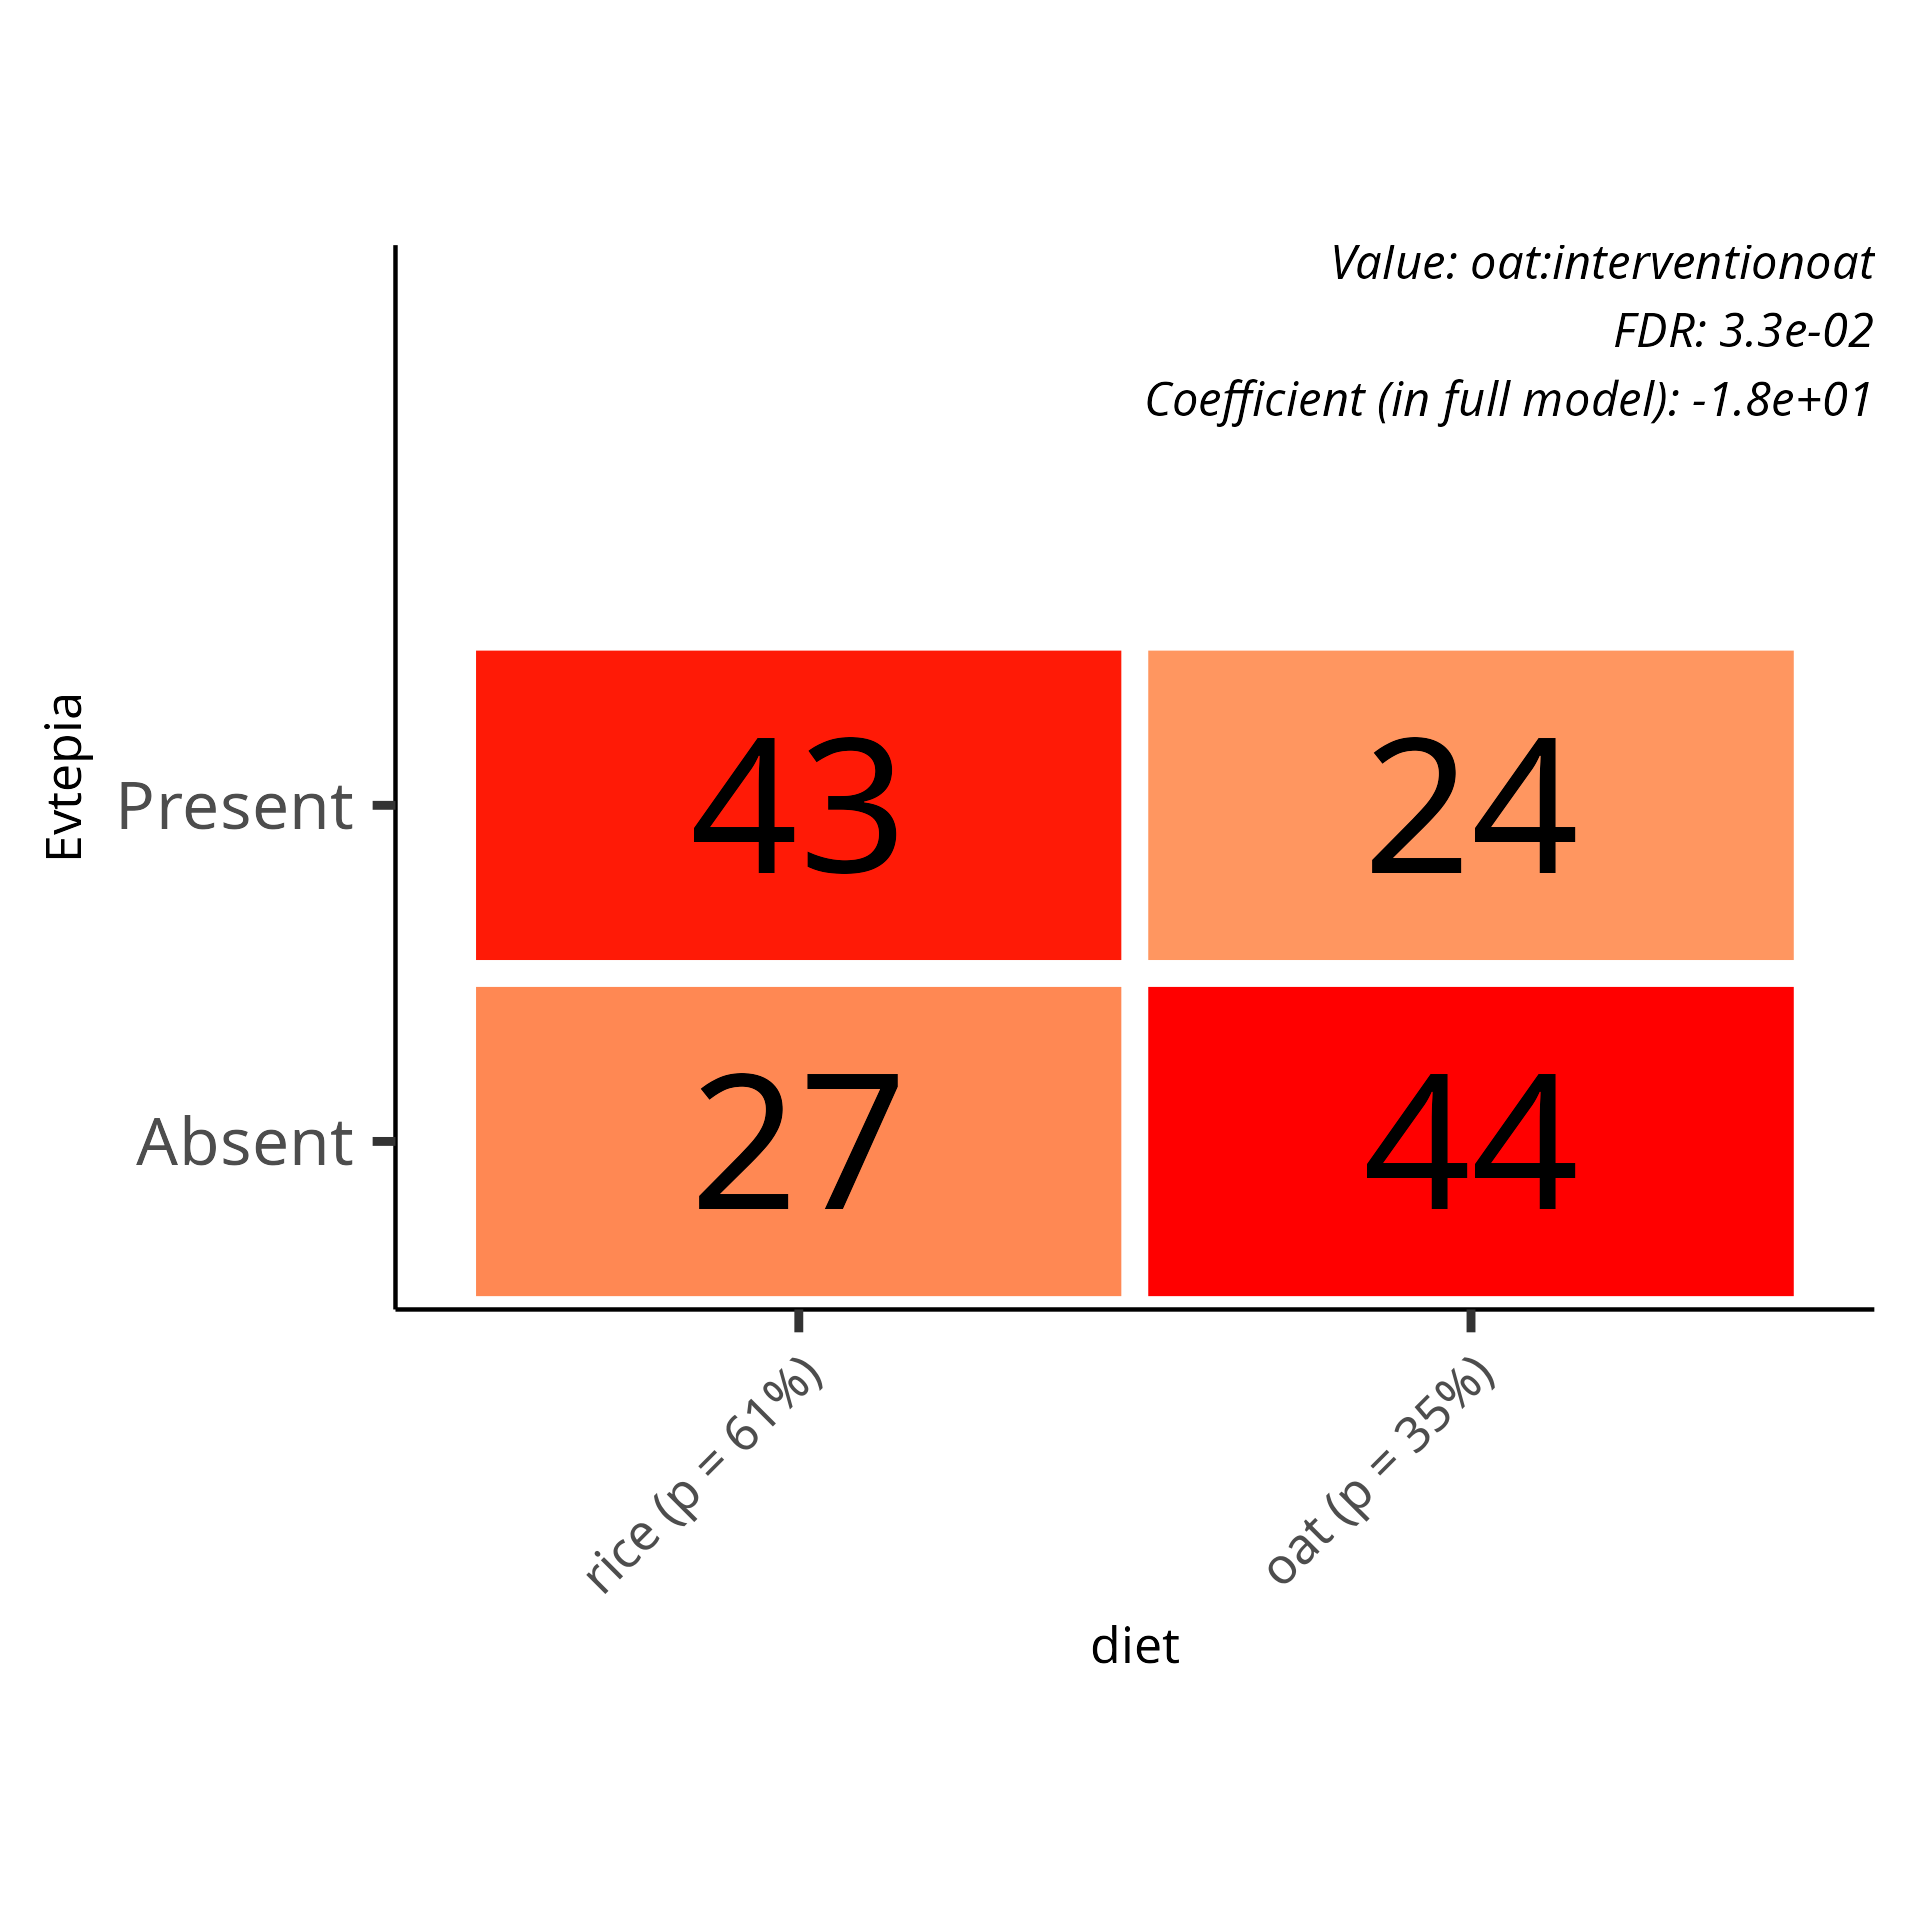
\includegraphics{../../output/daa/daa_taxa/genus/figures/association_plots/diet/logistic/diet_Evtepia_logistic.png}\\
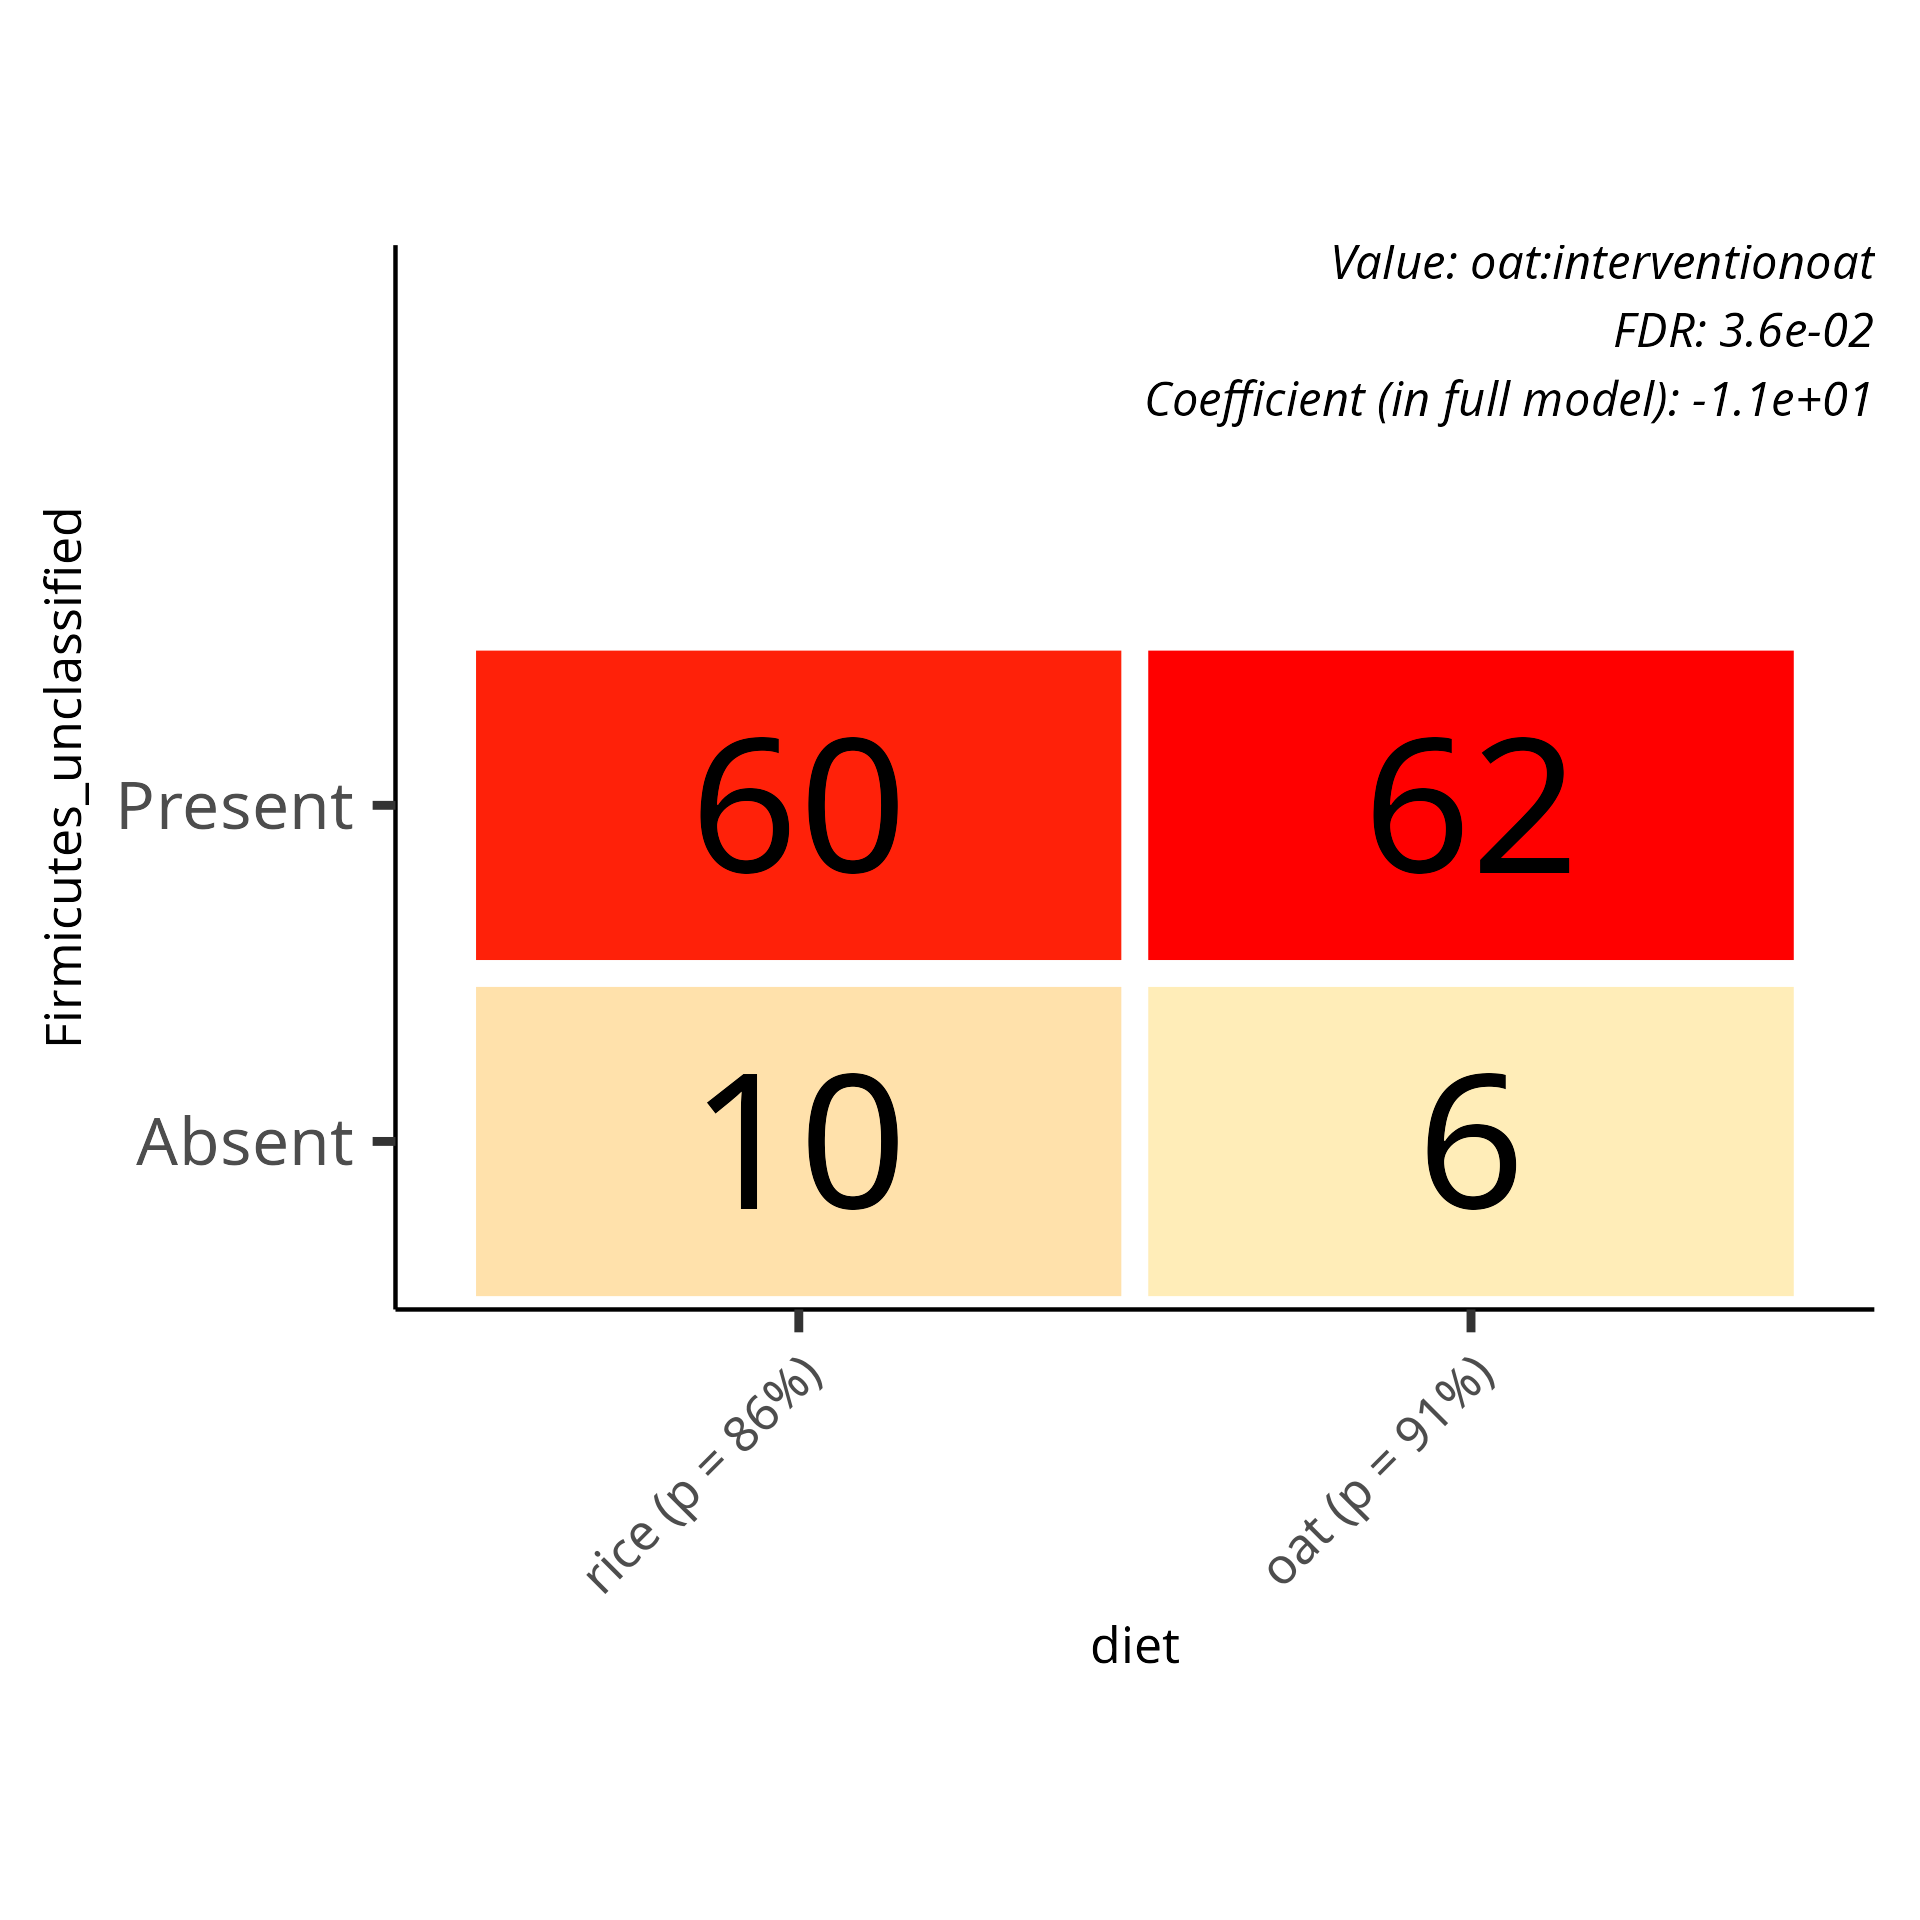
\includegraphics{../../output/daa/daa_taxa/genus/figures/association_plots/diet/logistic/diet_Firmicutes_unclassified_logistic.png}\\
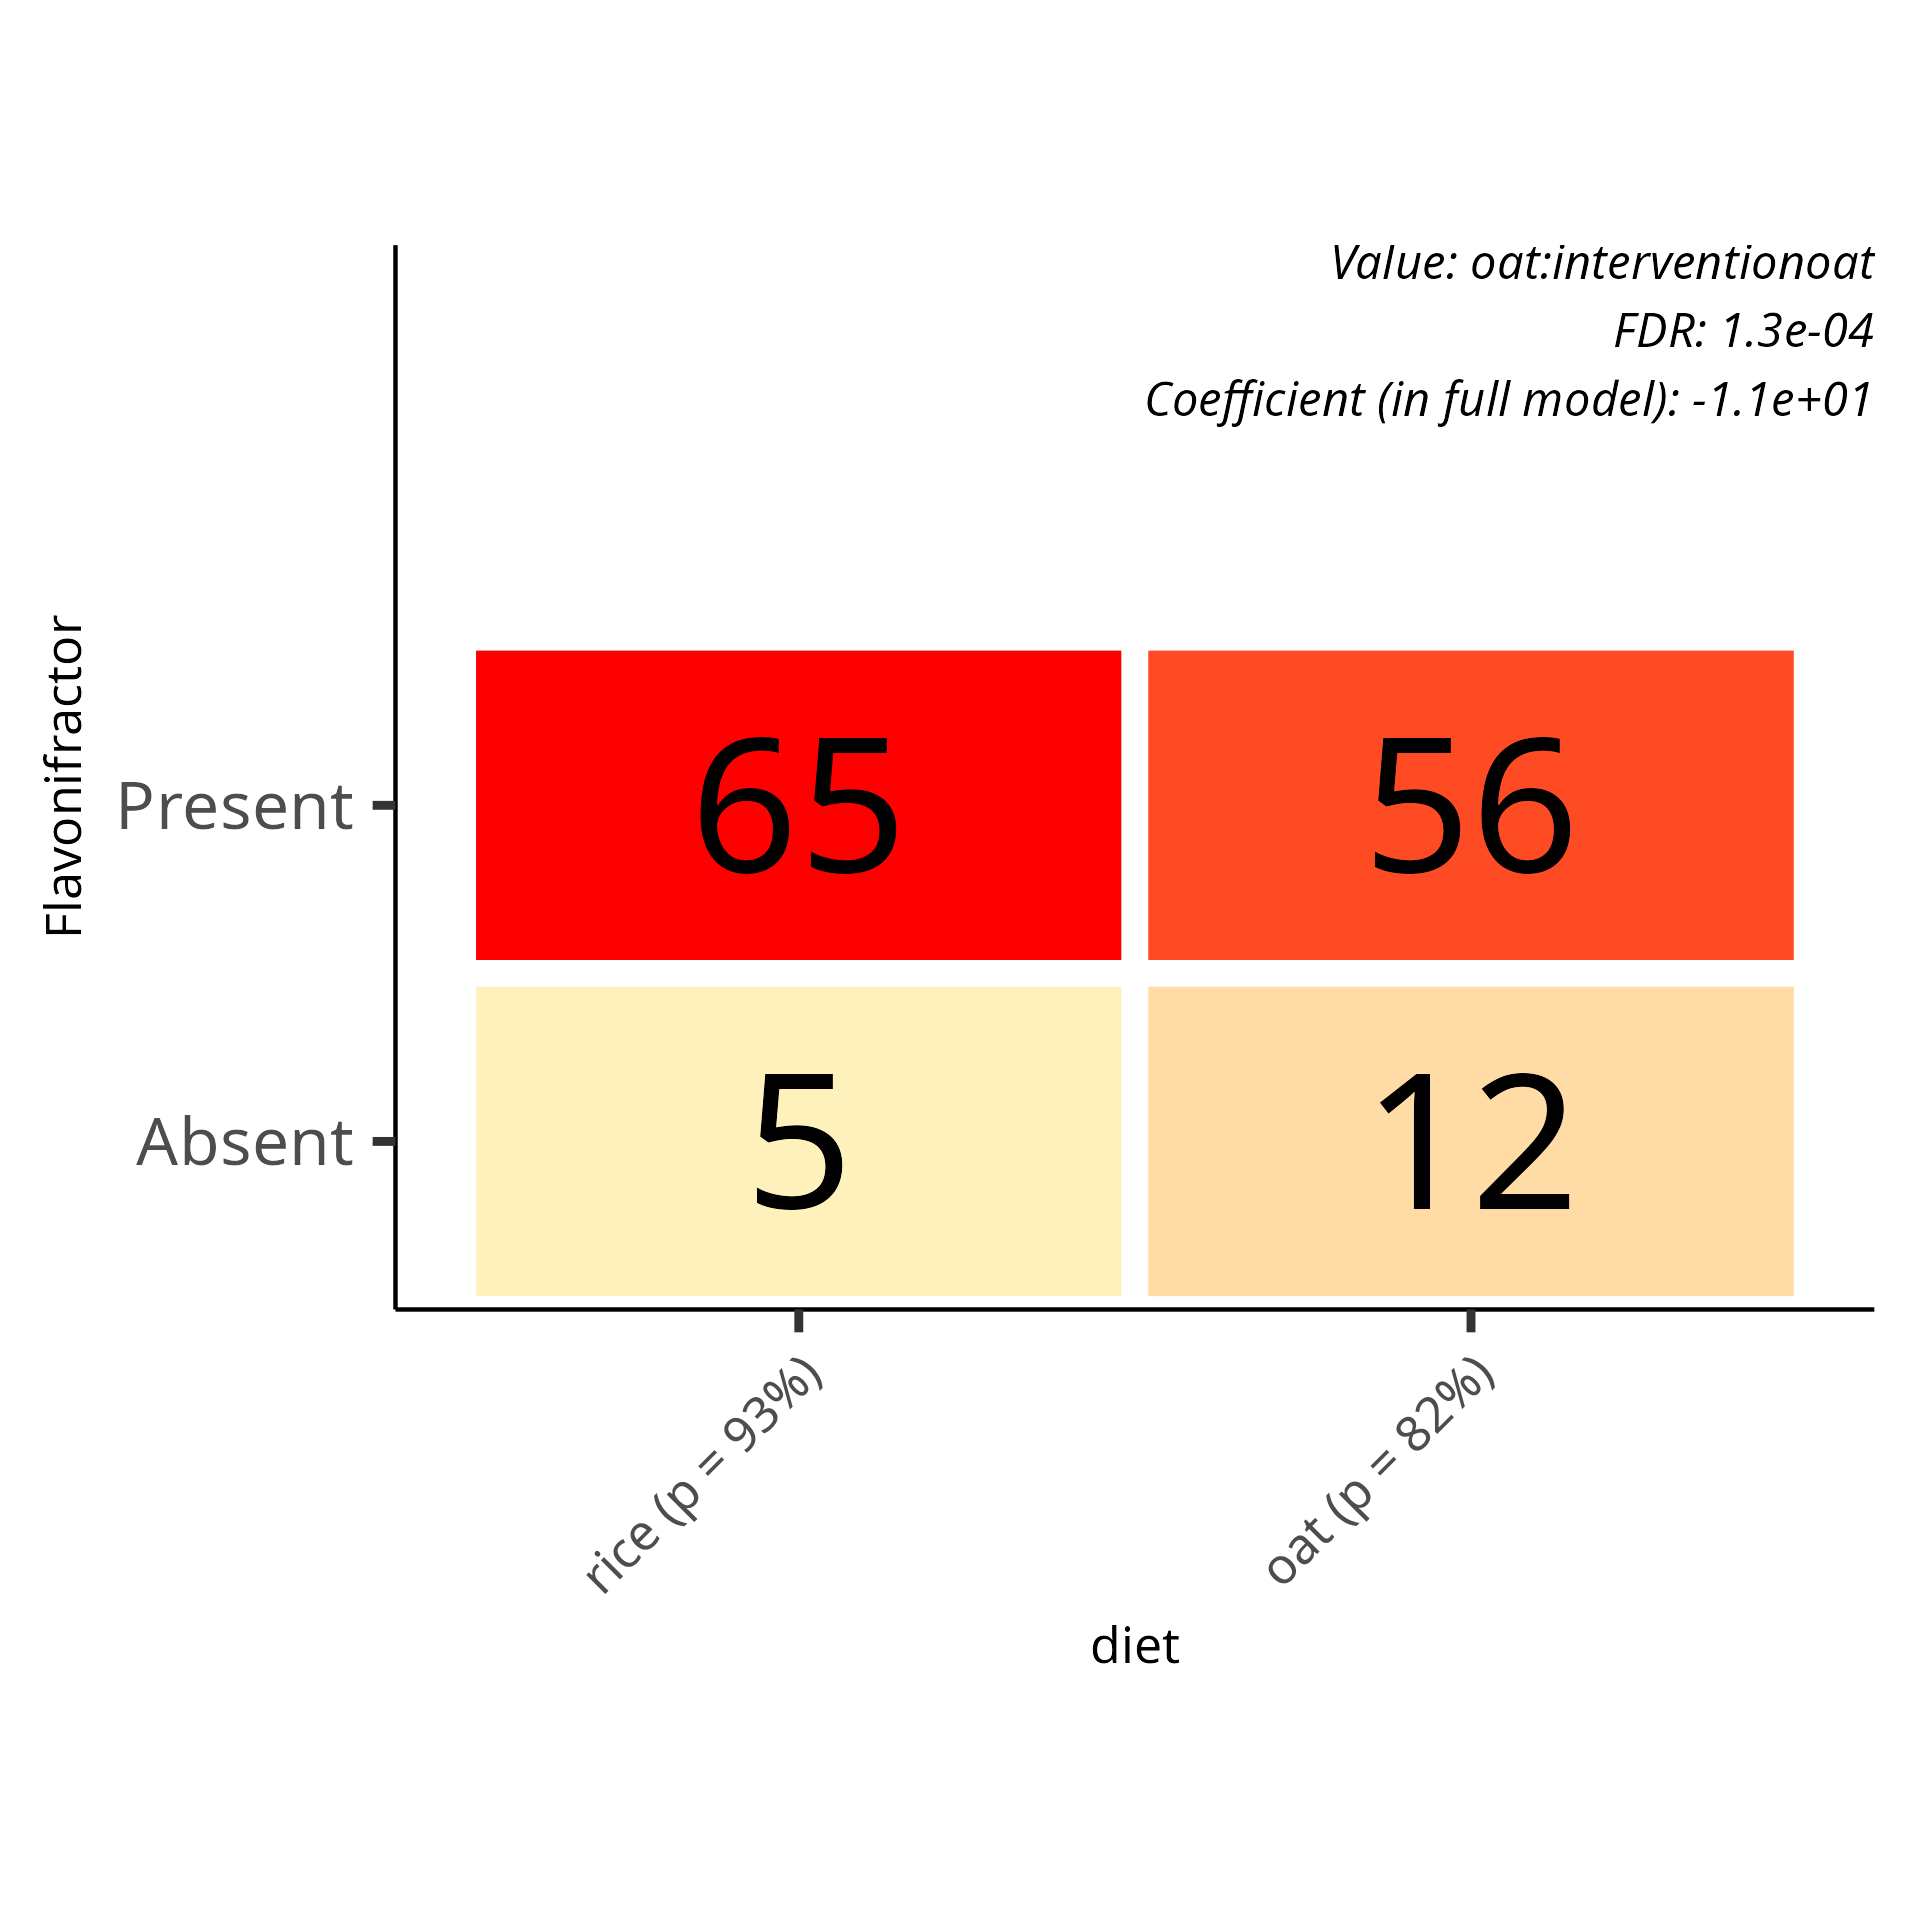
\includegraphics{../../output/daa/daa_taxa/genus/figures/association_plots/diet/logistic/diet_Flavonifractor_logistic.png}\\
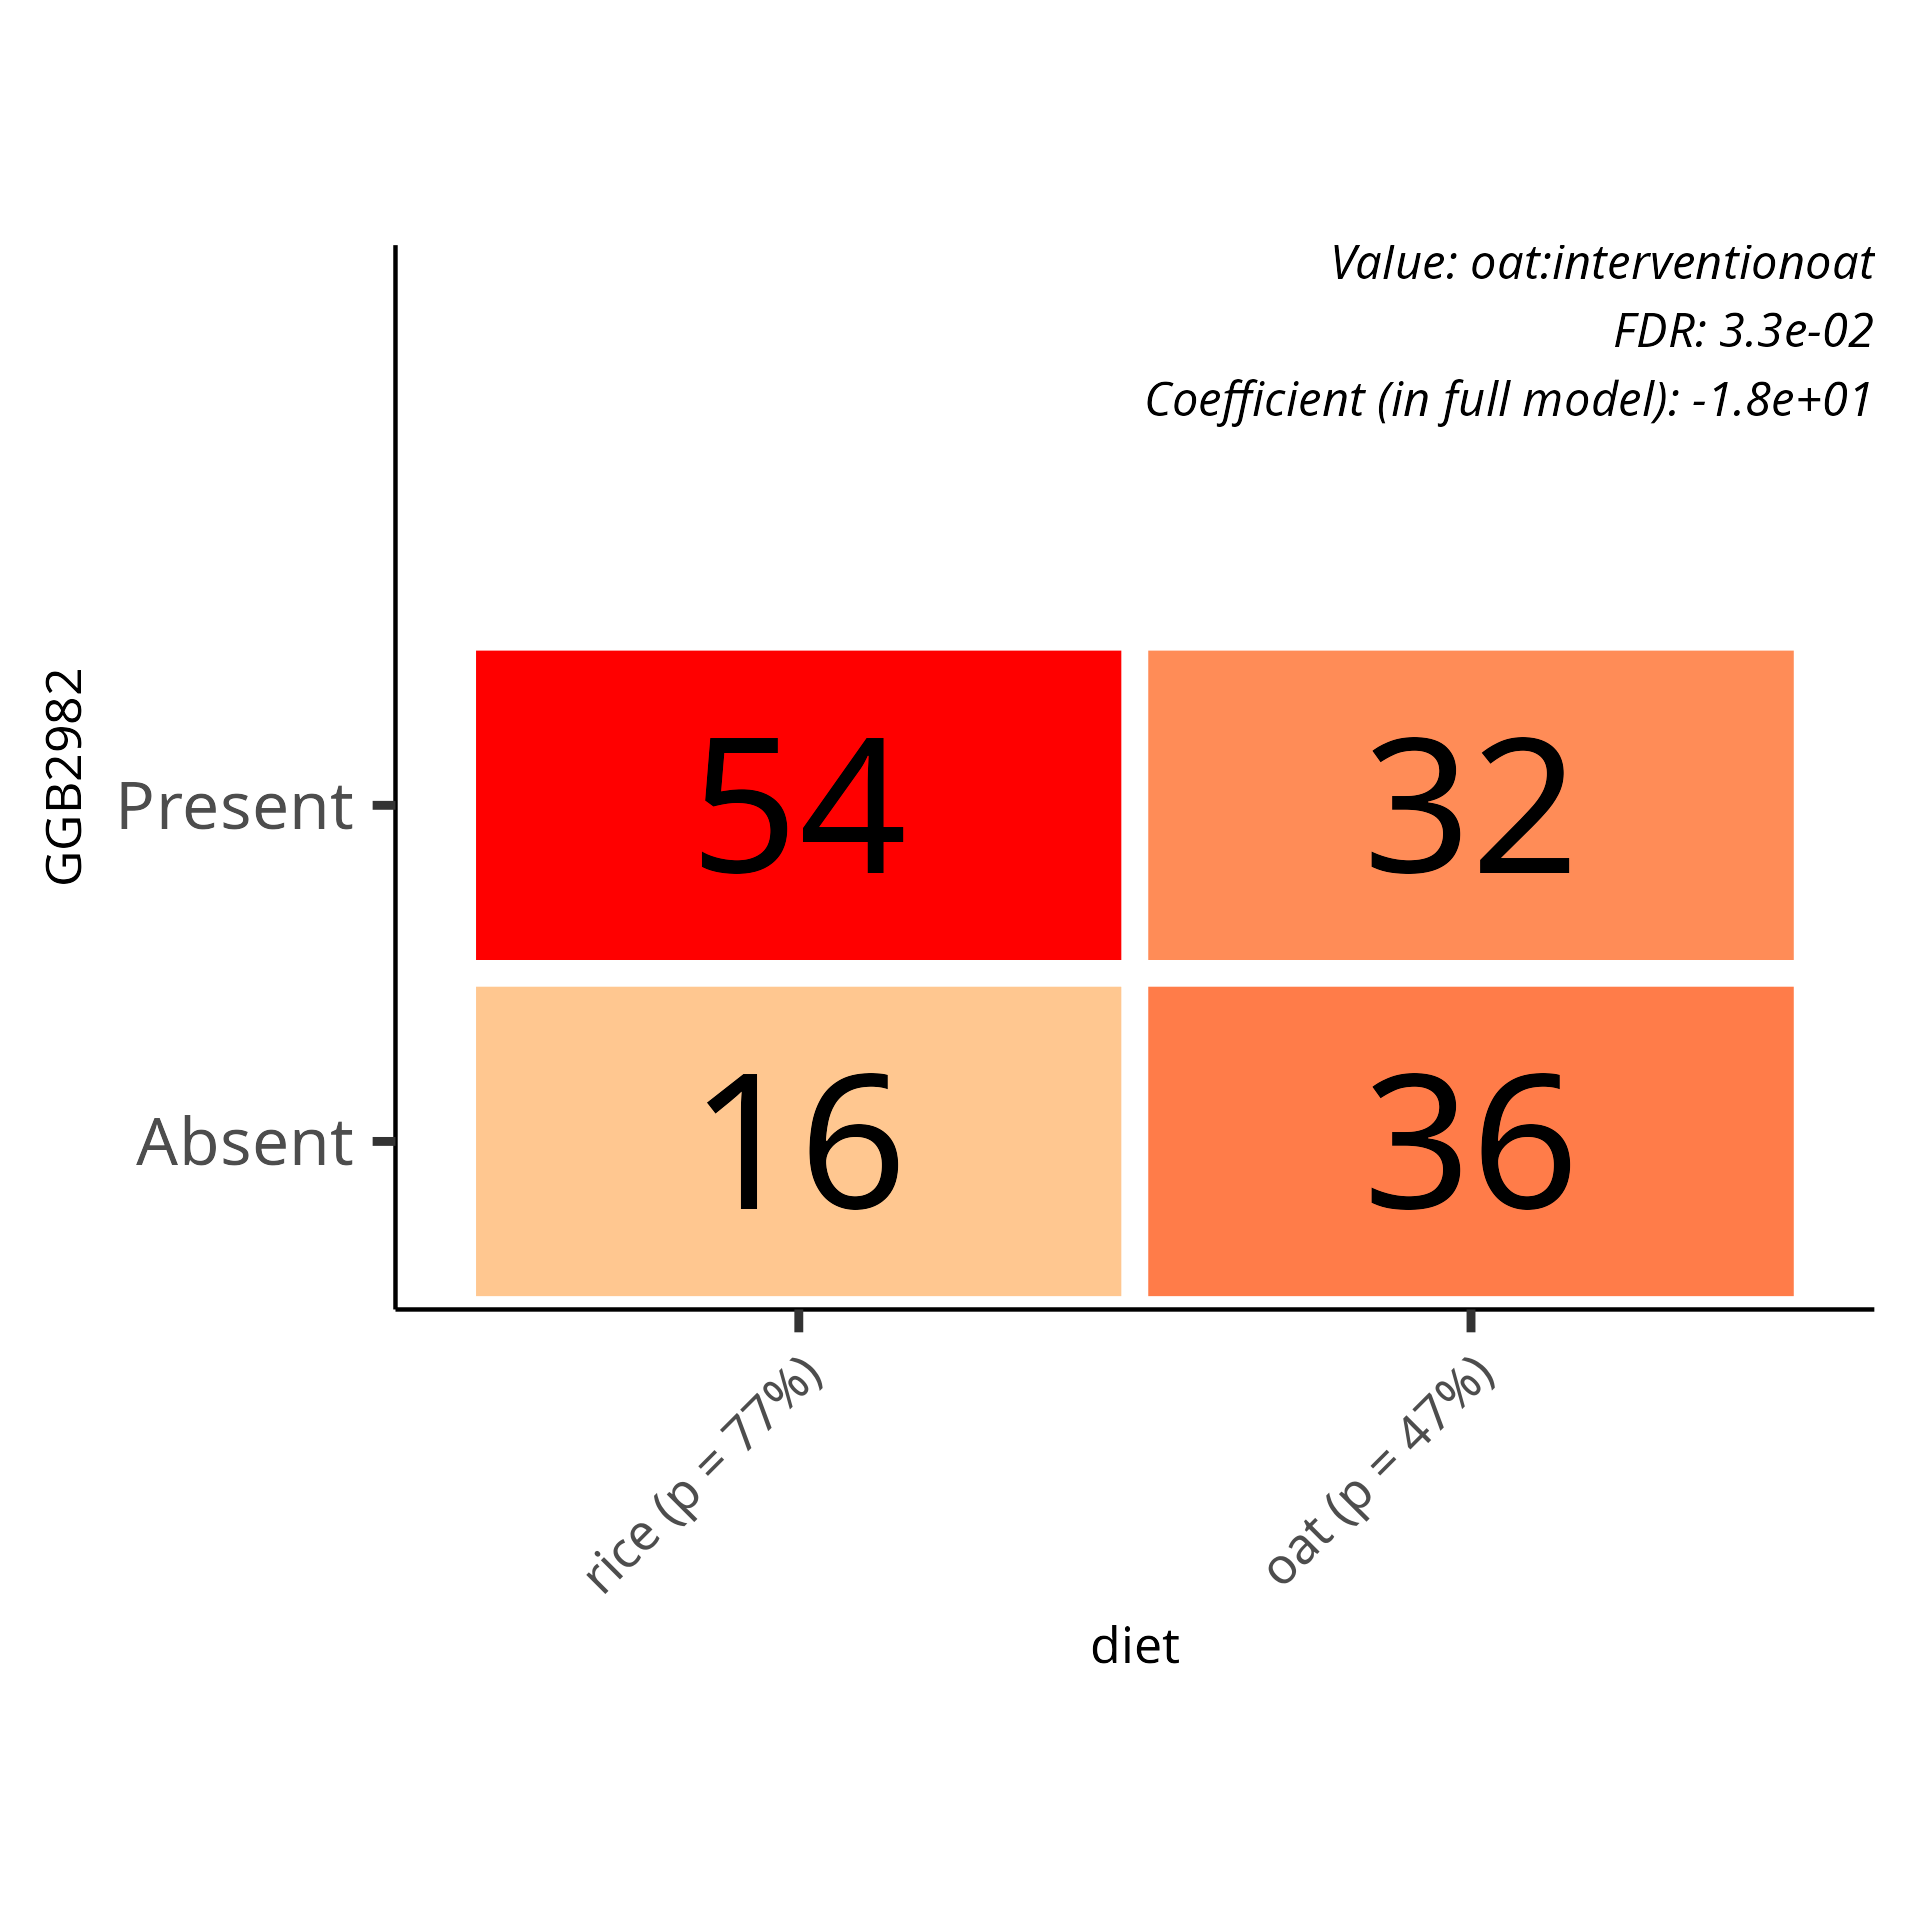
\includegraphics{../../output/daa/daa_taxa/genus/figures/association_plots/diet/logistic/diet_GGB2982_logistic.png}\\
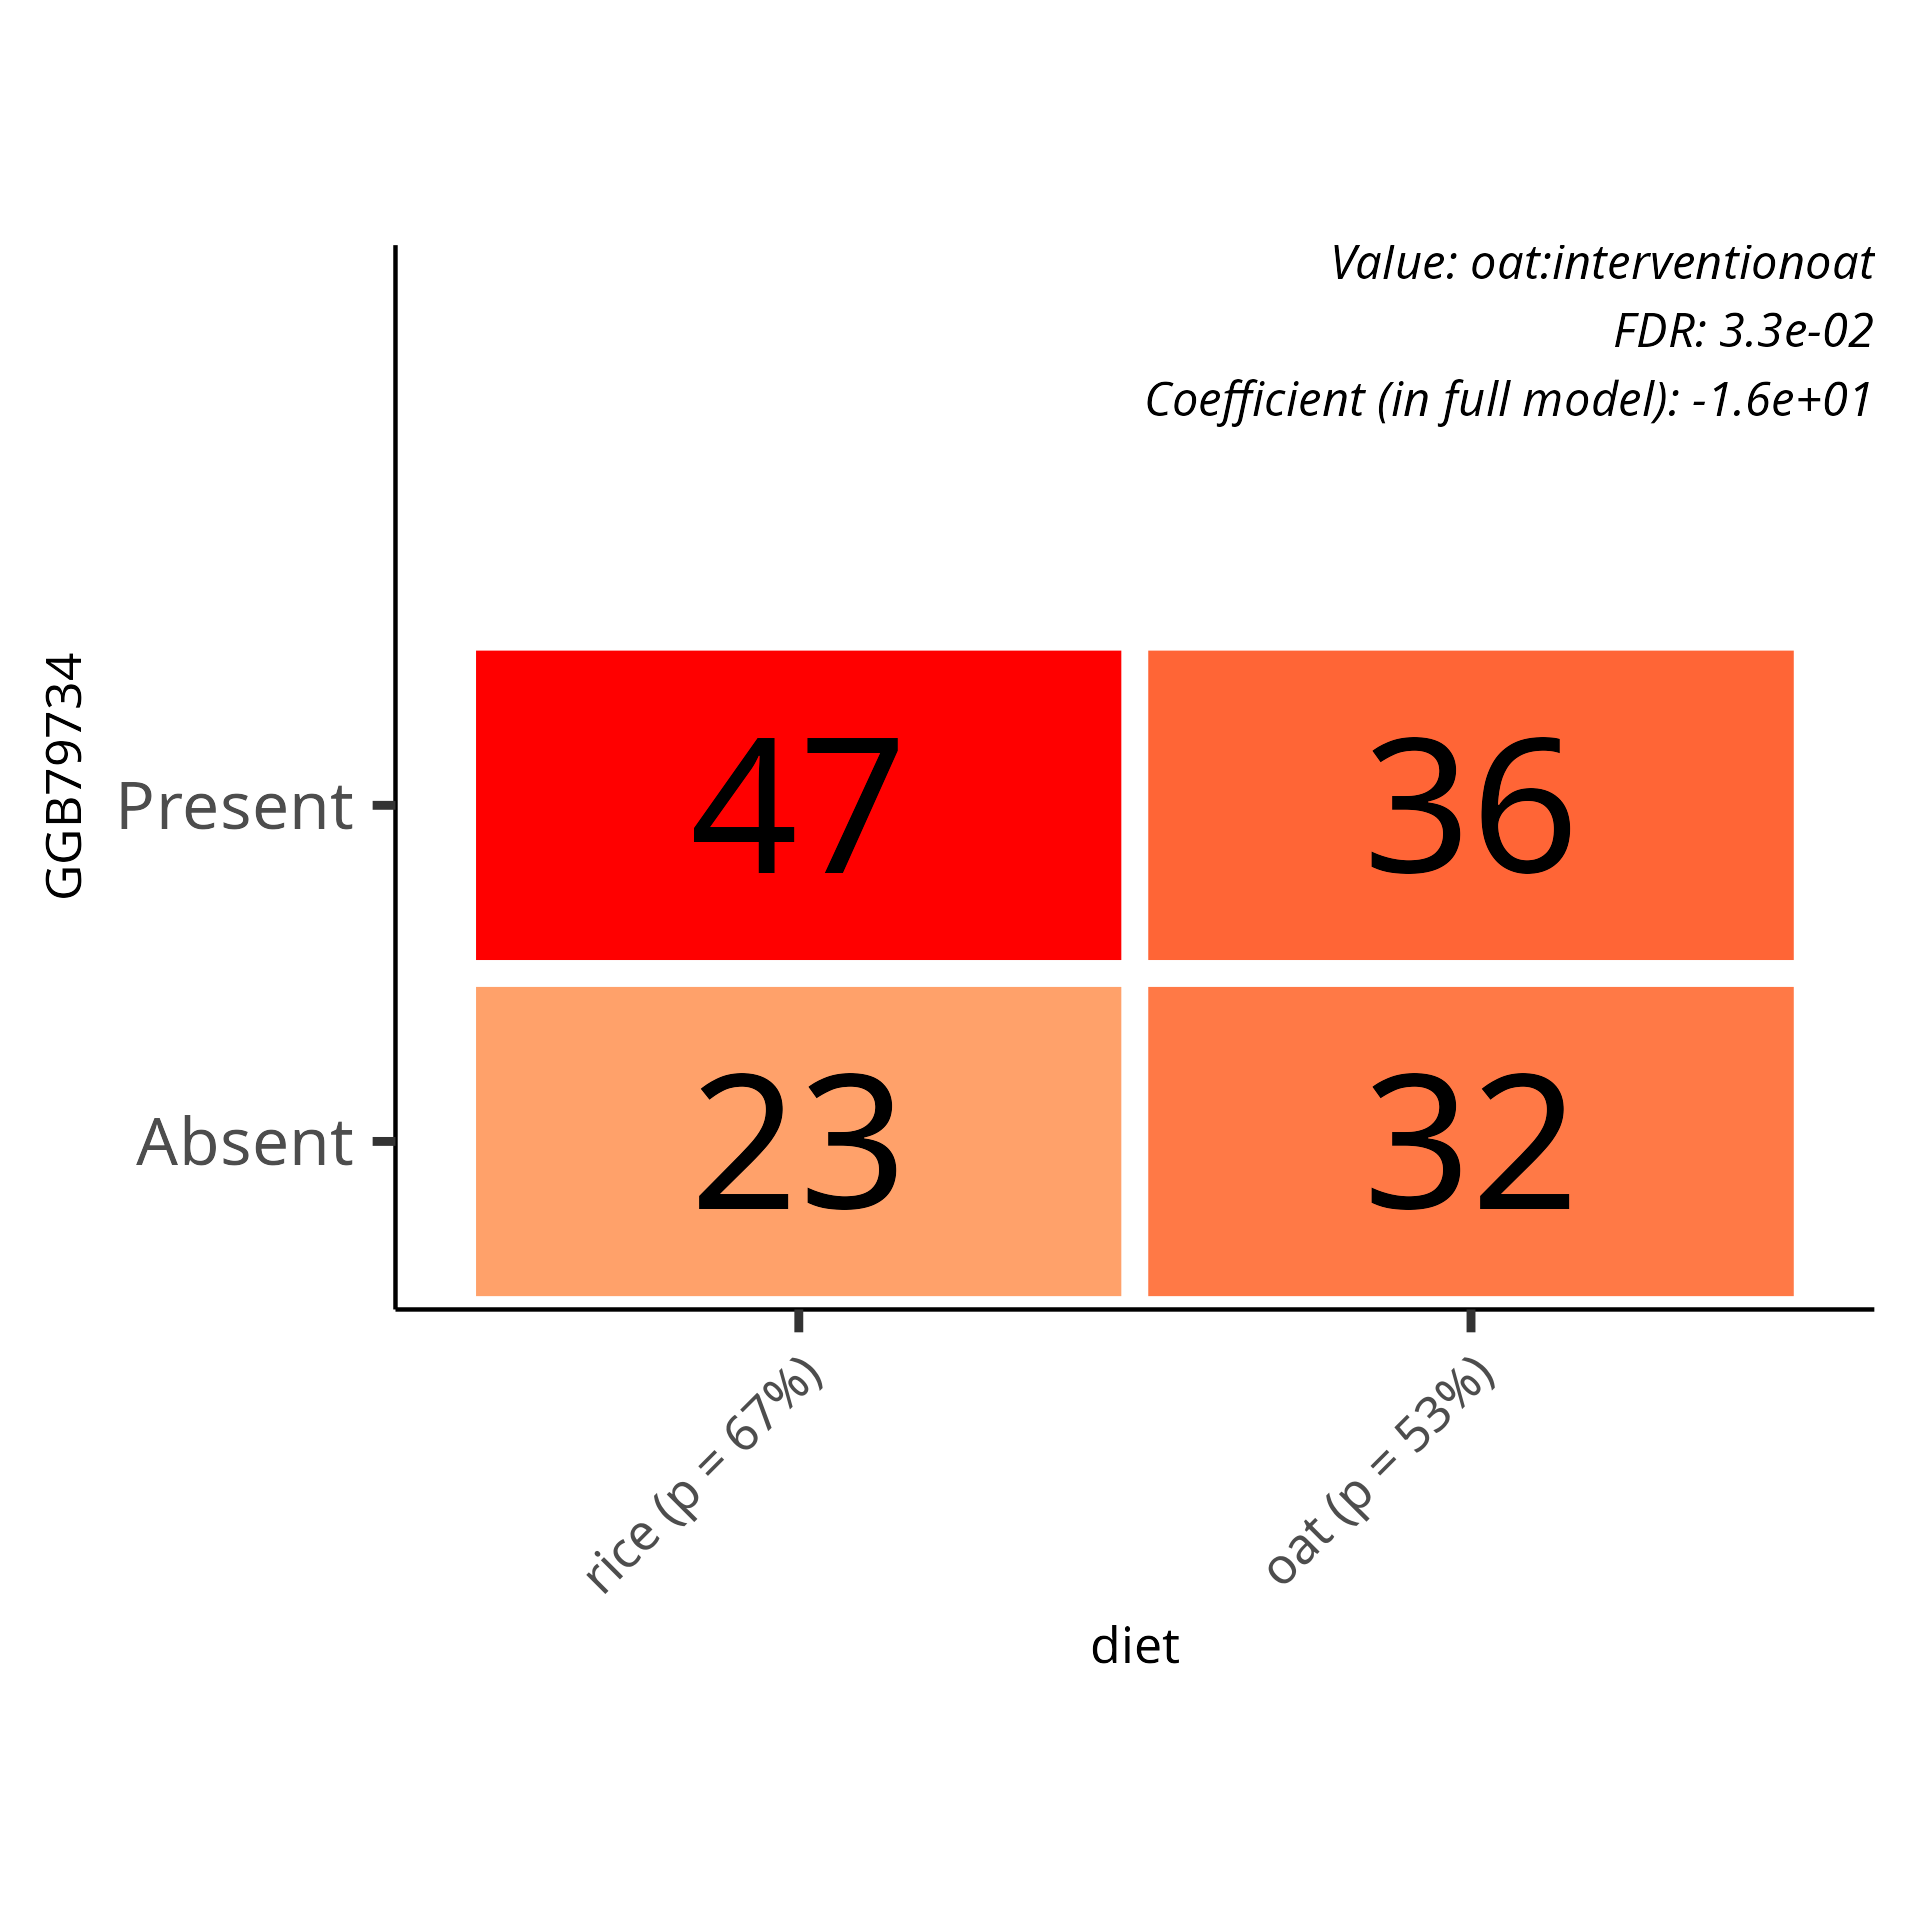
\includegraphics{../../output/daa/daa_taxa/genus/figures/association_plots/diet/logistic/diet_GGB79734_logistic.png}\\
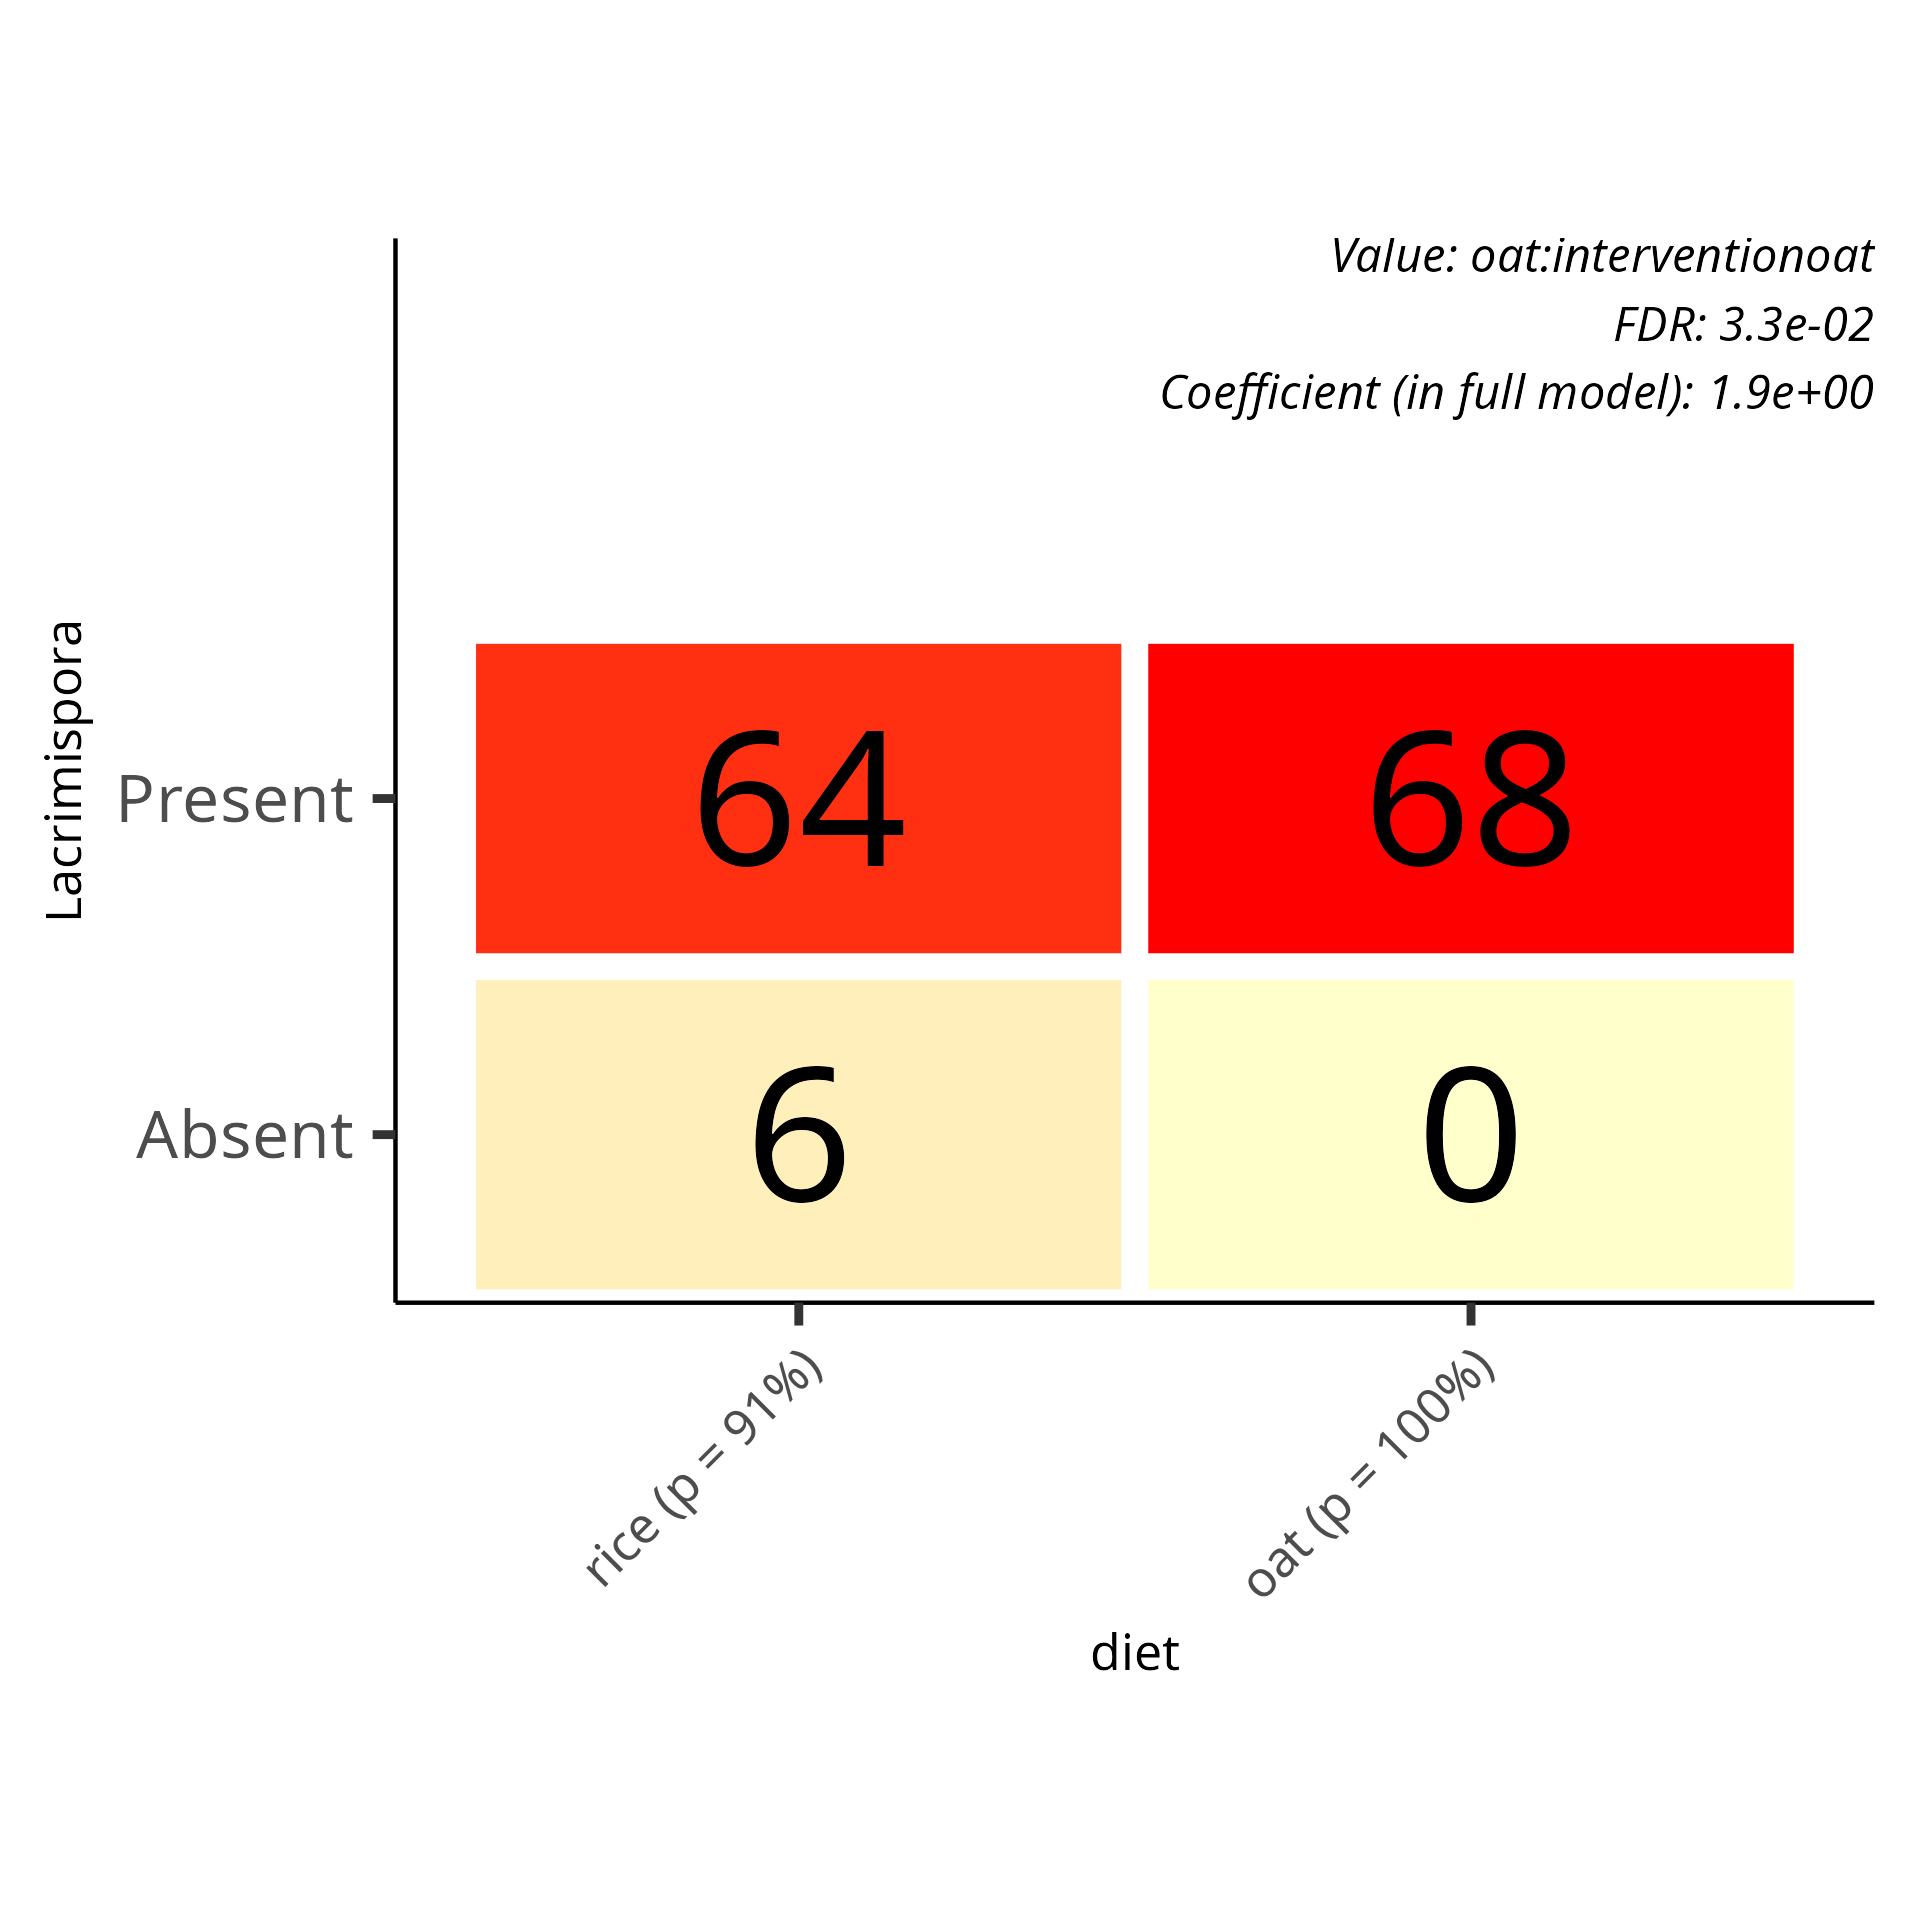
\includegraphics{../../output/daa/daa_taxa/genus/figures/association_plots/diet/logistic/diet_Lacrimispora_logistic.png}\\
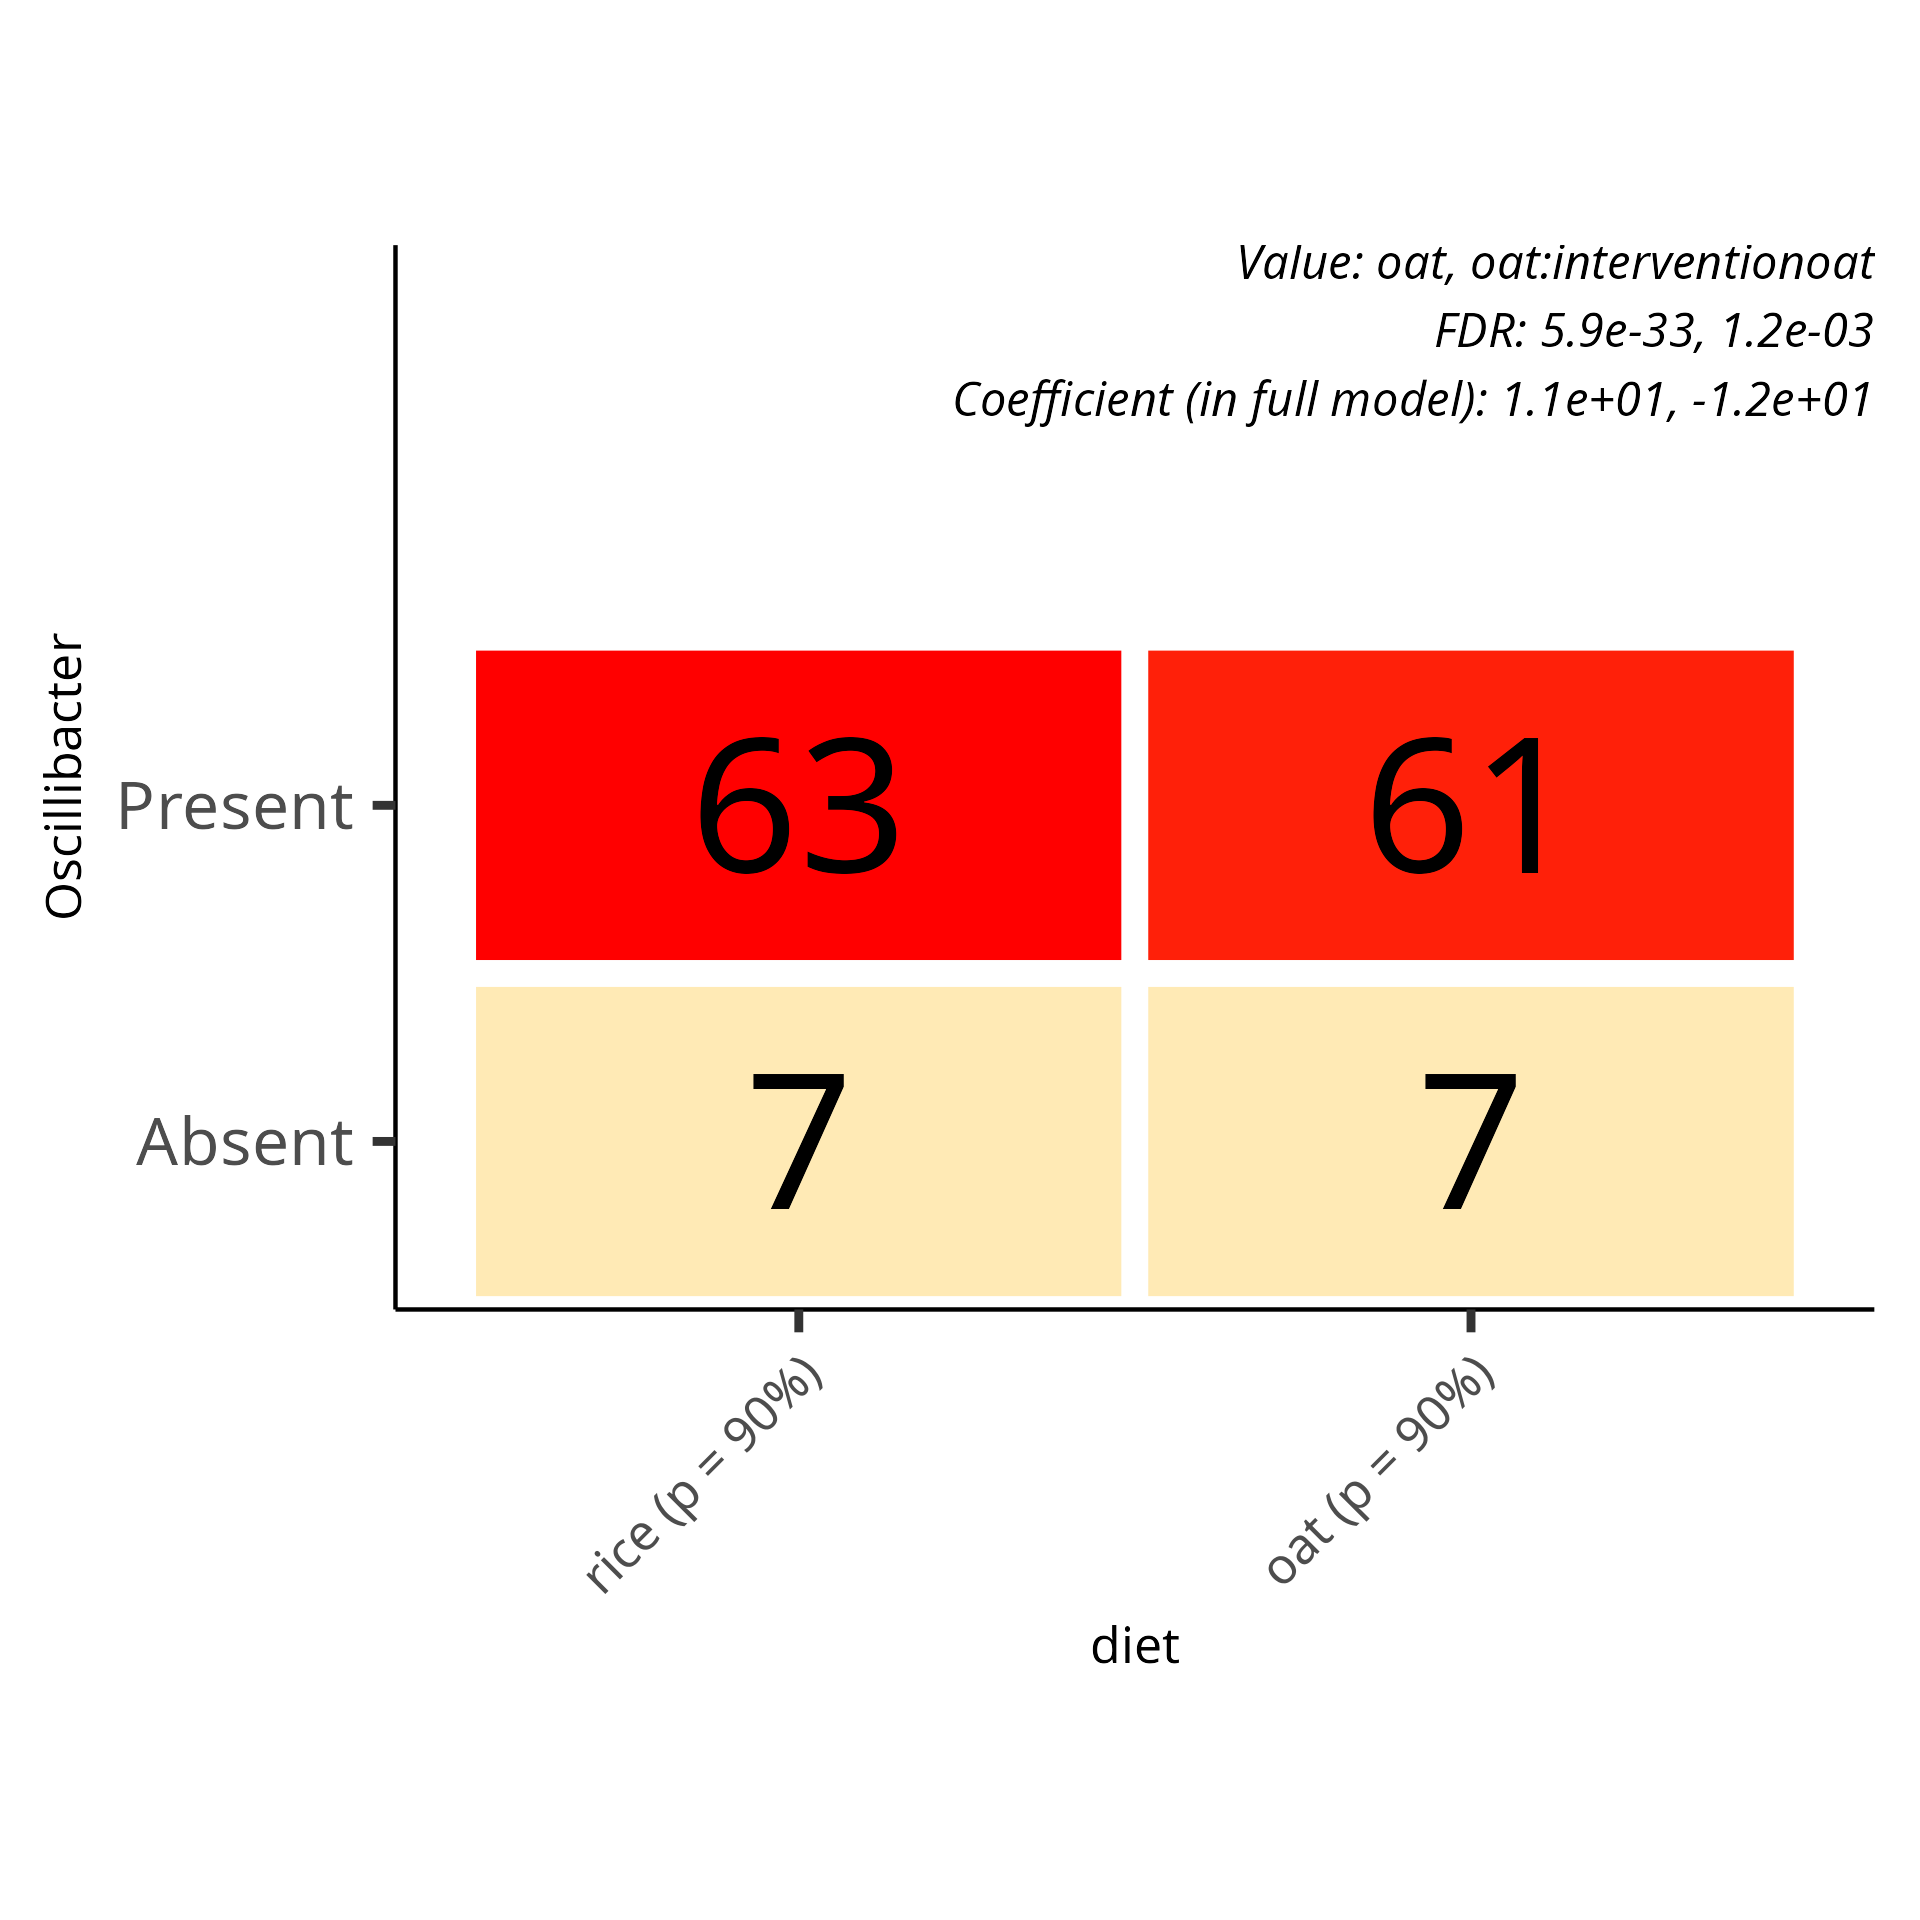
\includegraphics{../../output/daa/daa_taxa/genus/figures/association_plots/diet/logistic/diet_Oscillibacter_logistic.png}\\
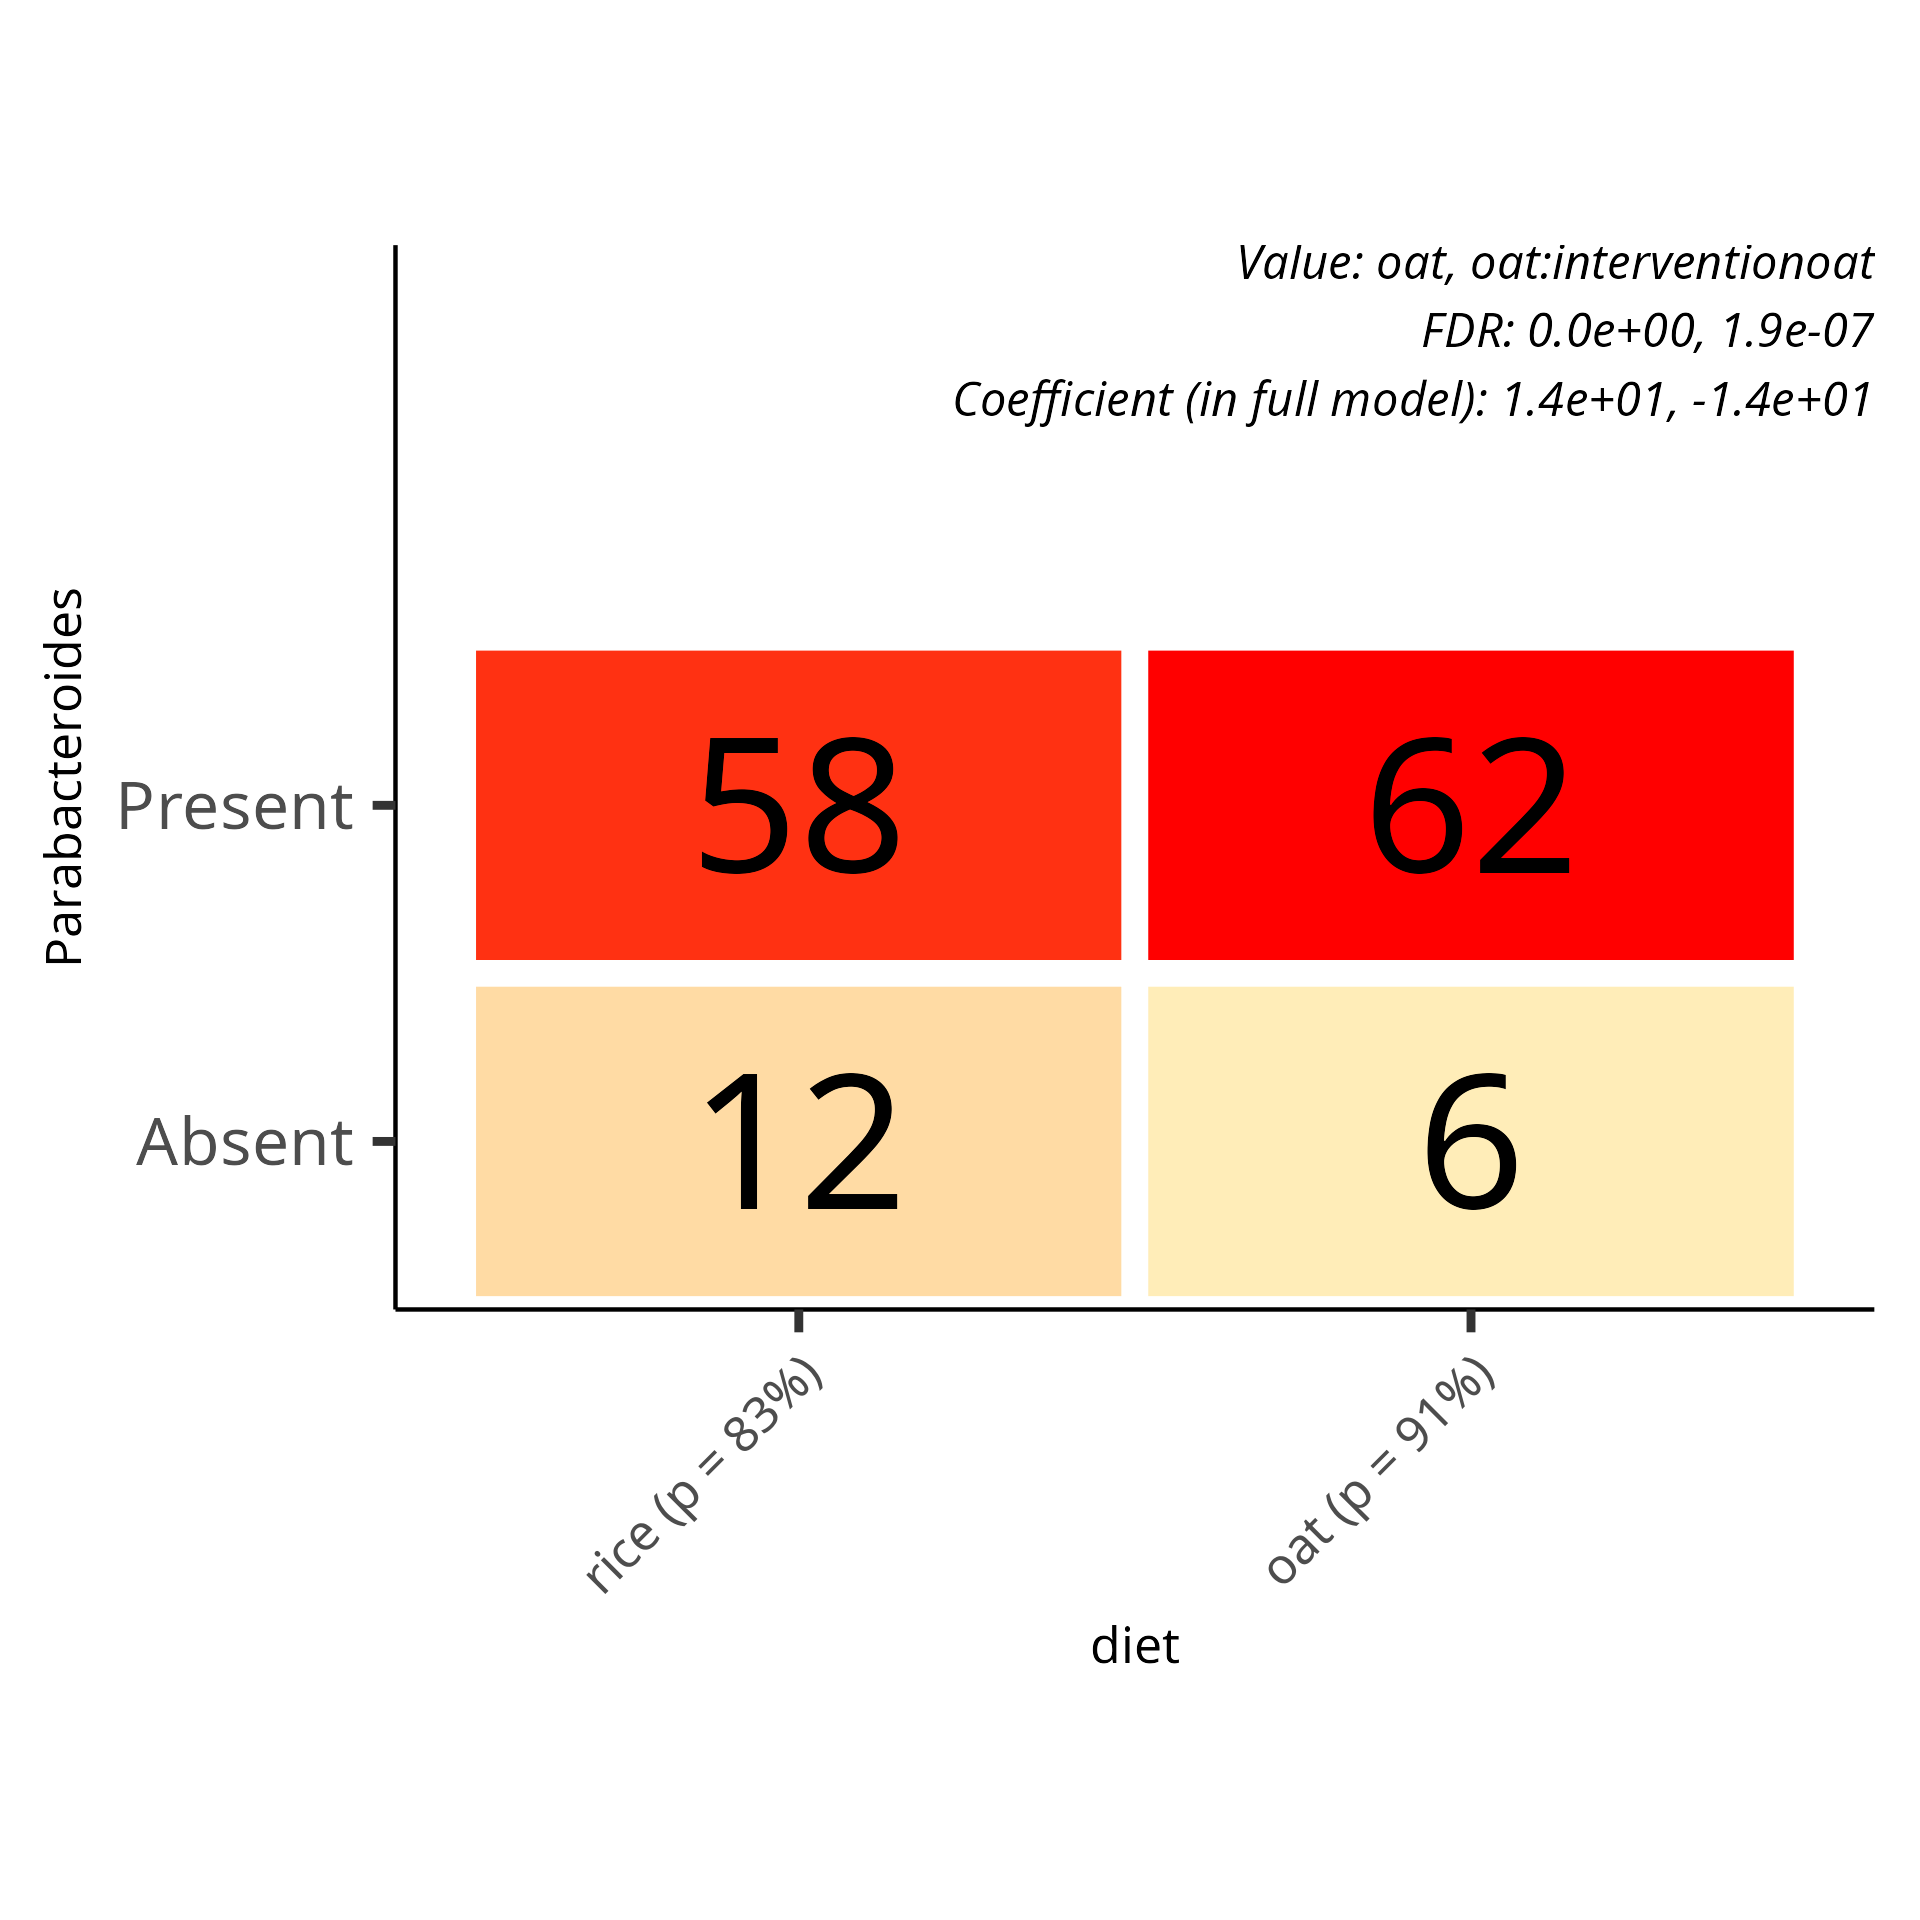
\includegraphics{../../output/daa/daa_taxa/genus/figures/association_plots/diet/logistic/diet_Parabacteroides_logistic.png}\\
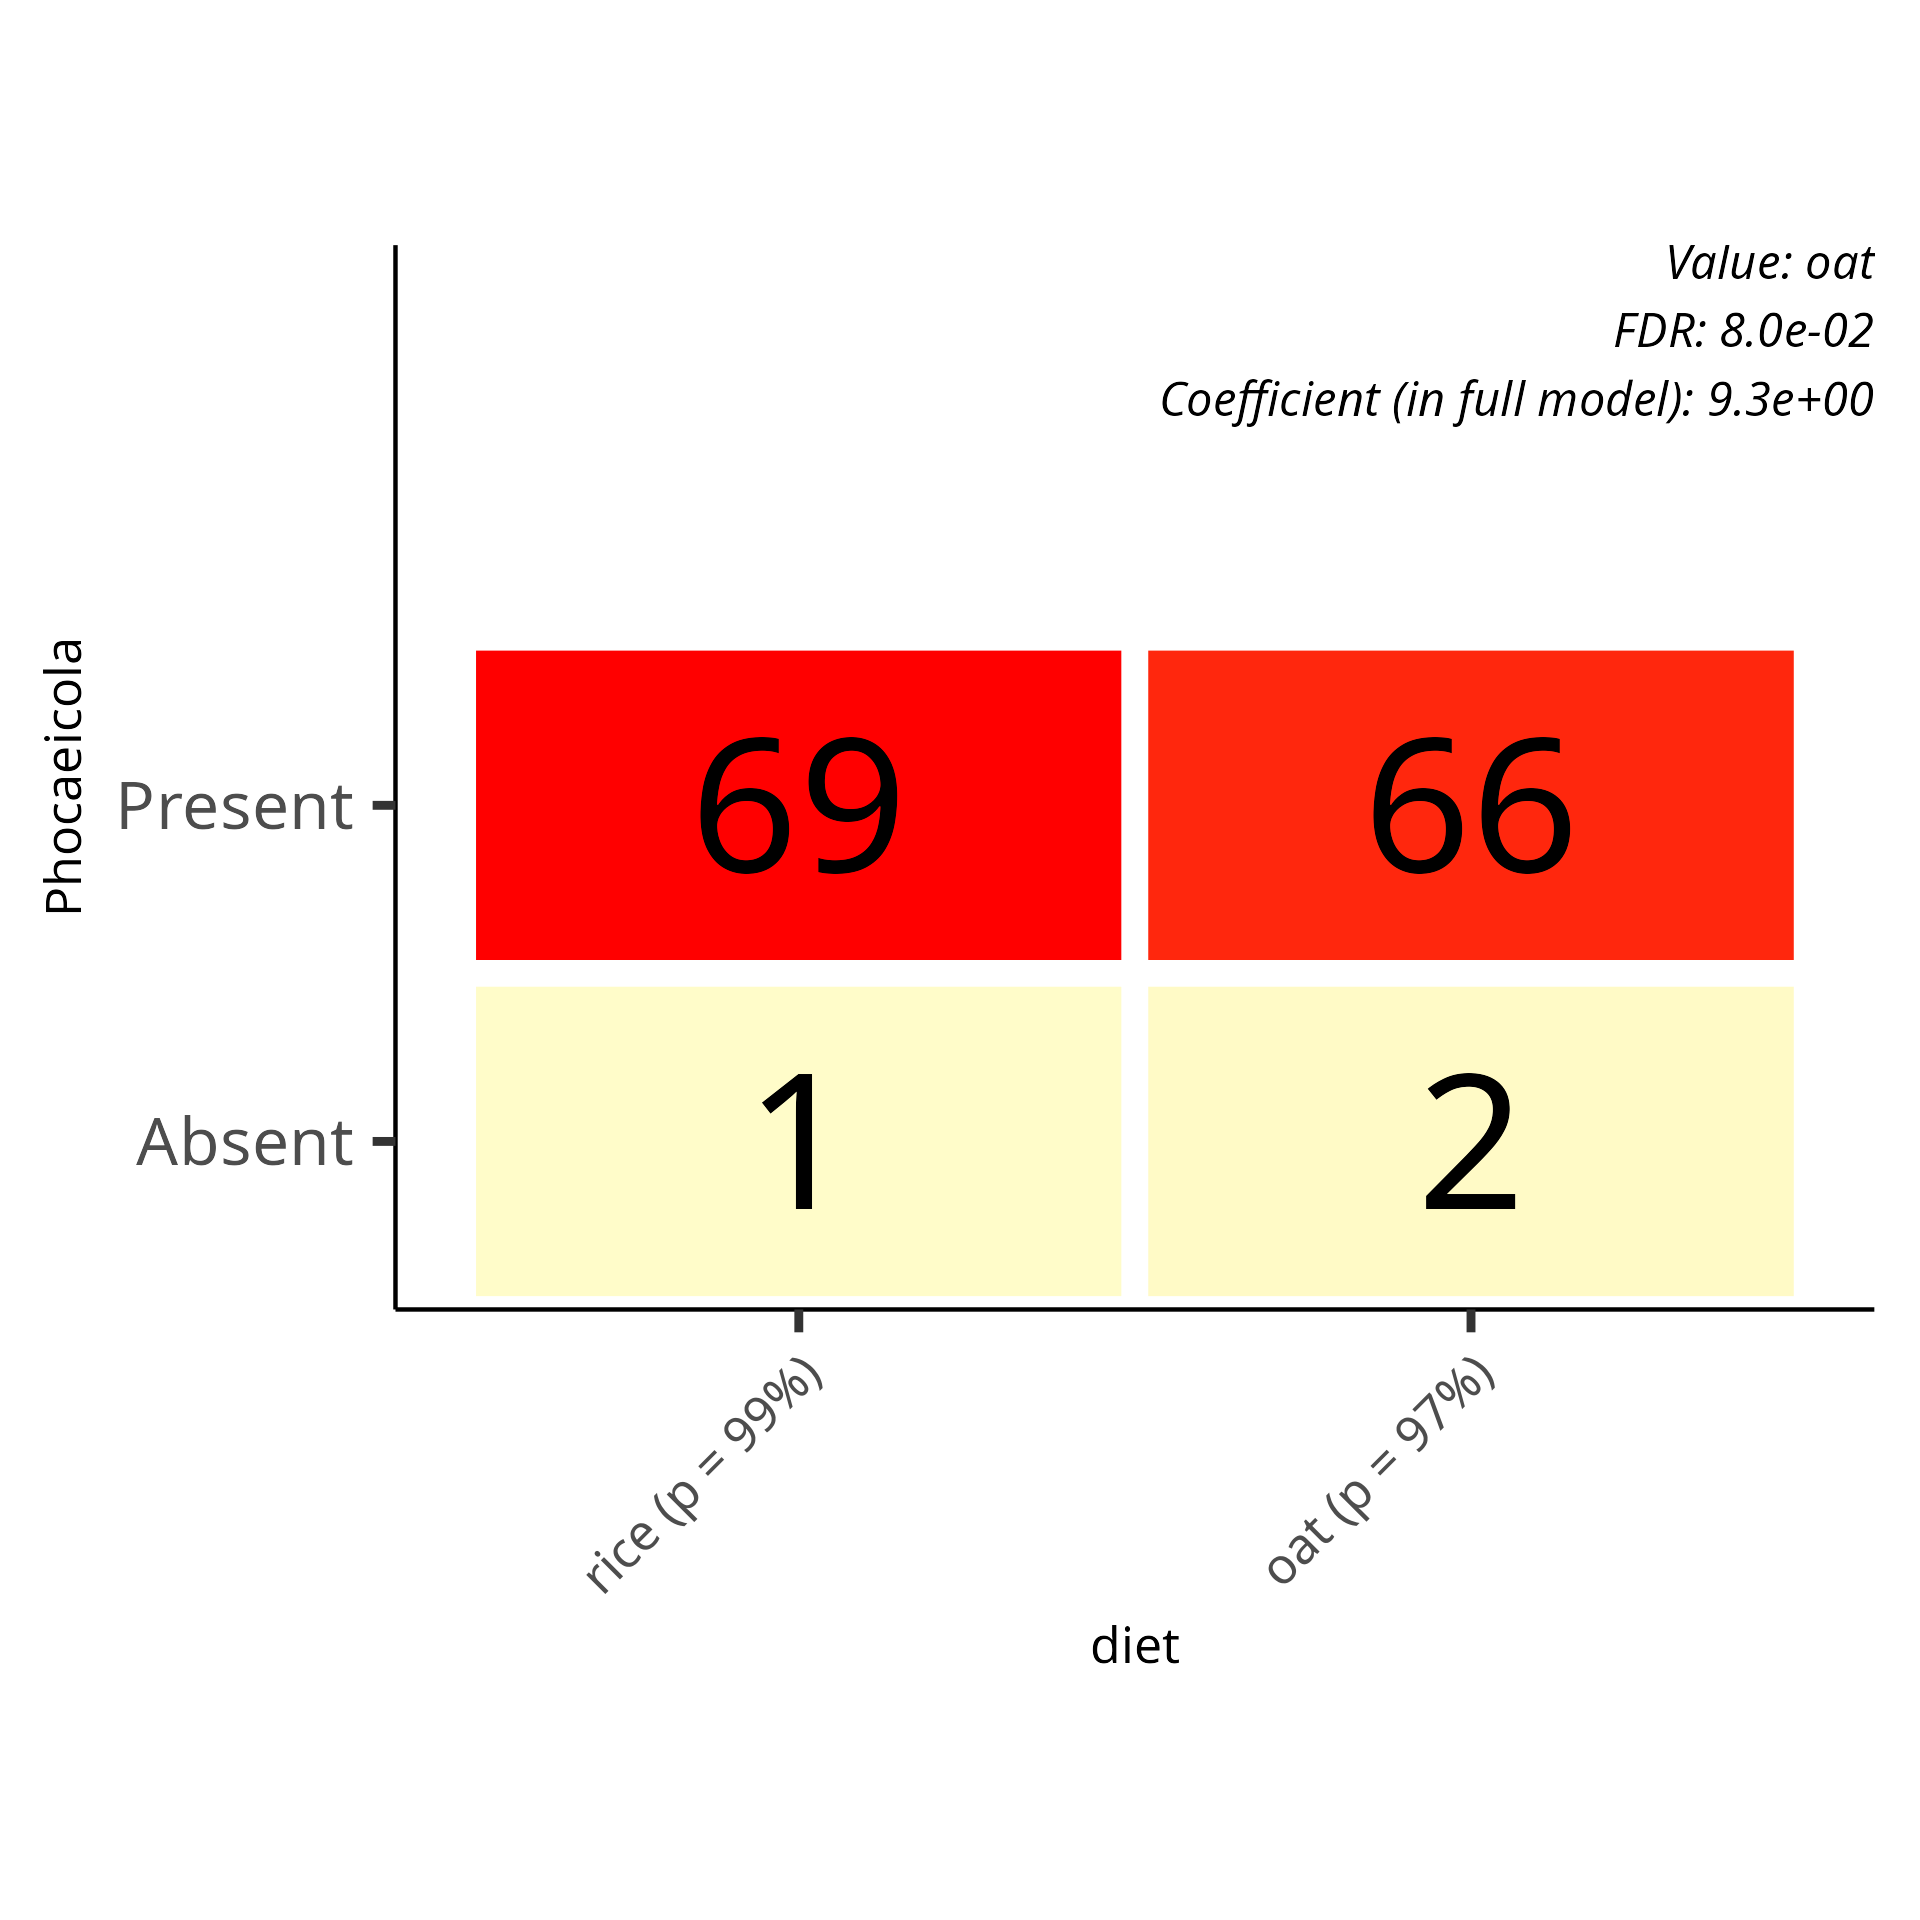
\includegraphics{../../output/daa/daa_taxa/genus/figures/association_plots/diet/logistic/diet_Phocaeicola_logistic.png}\\
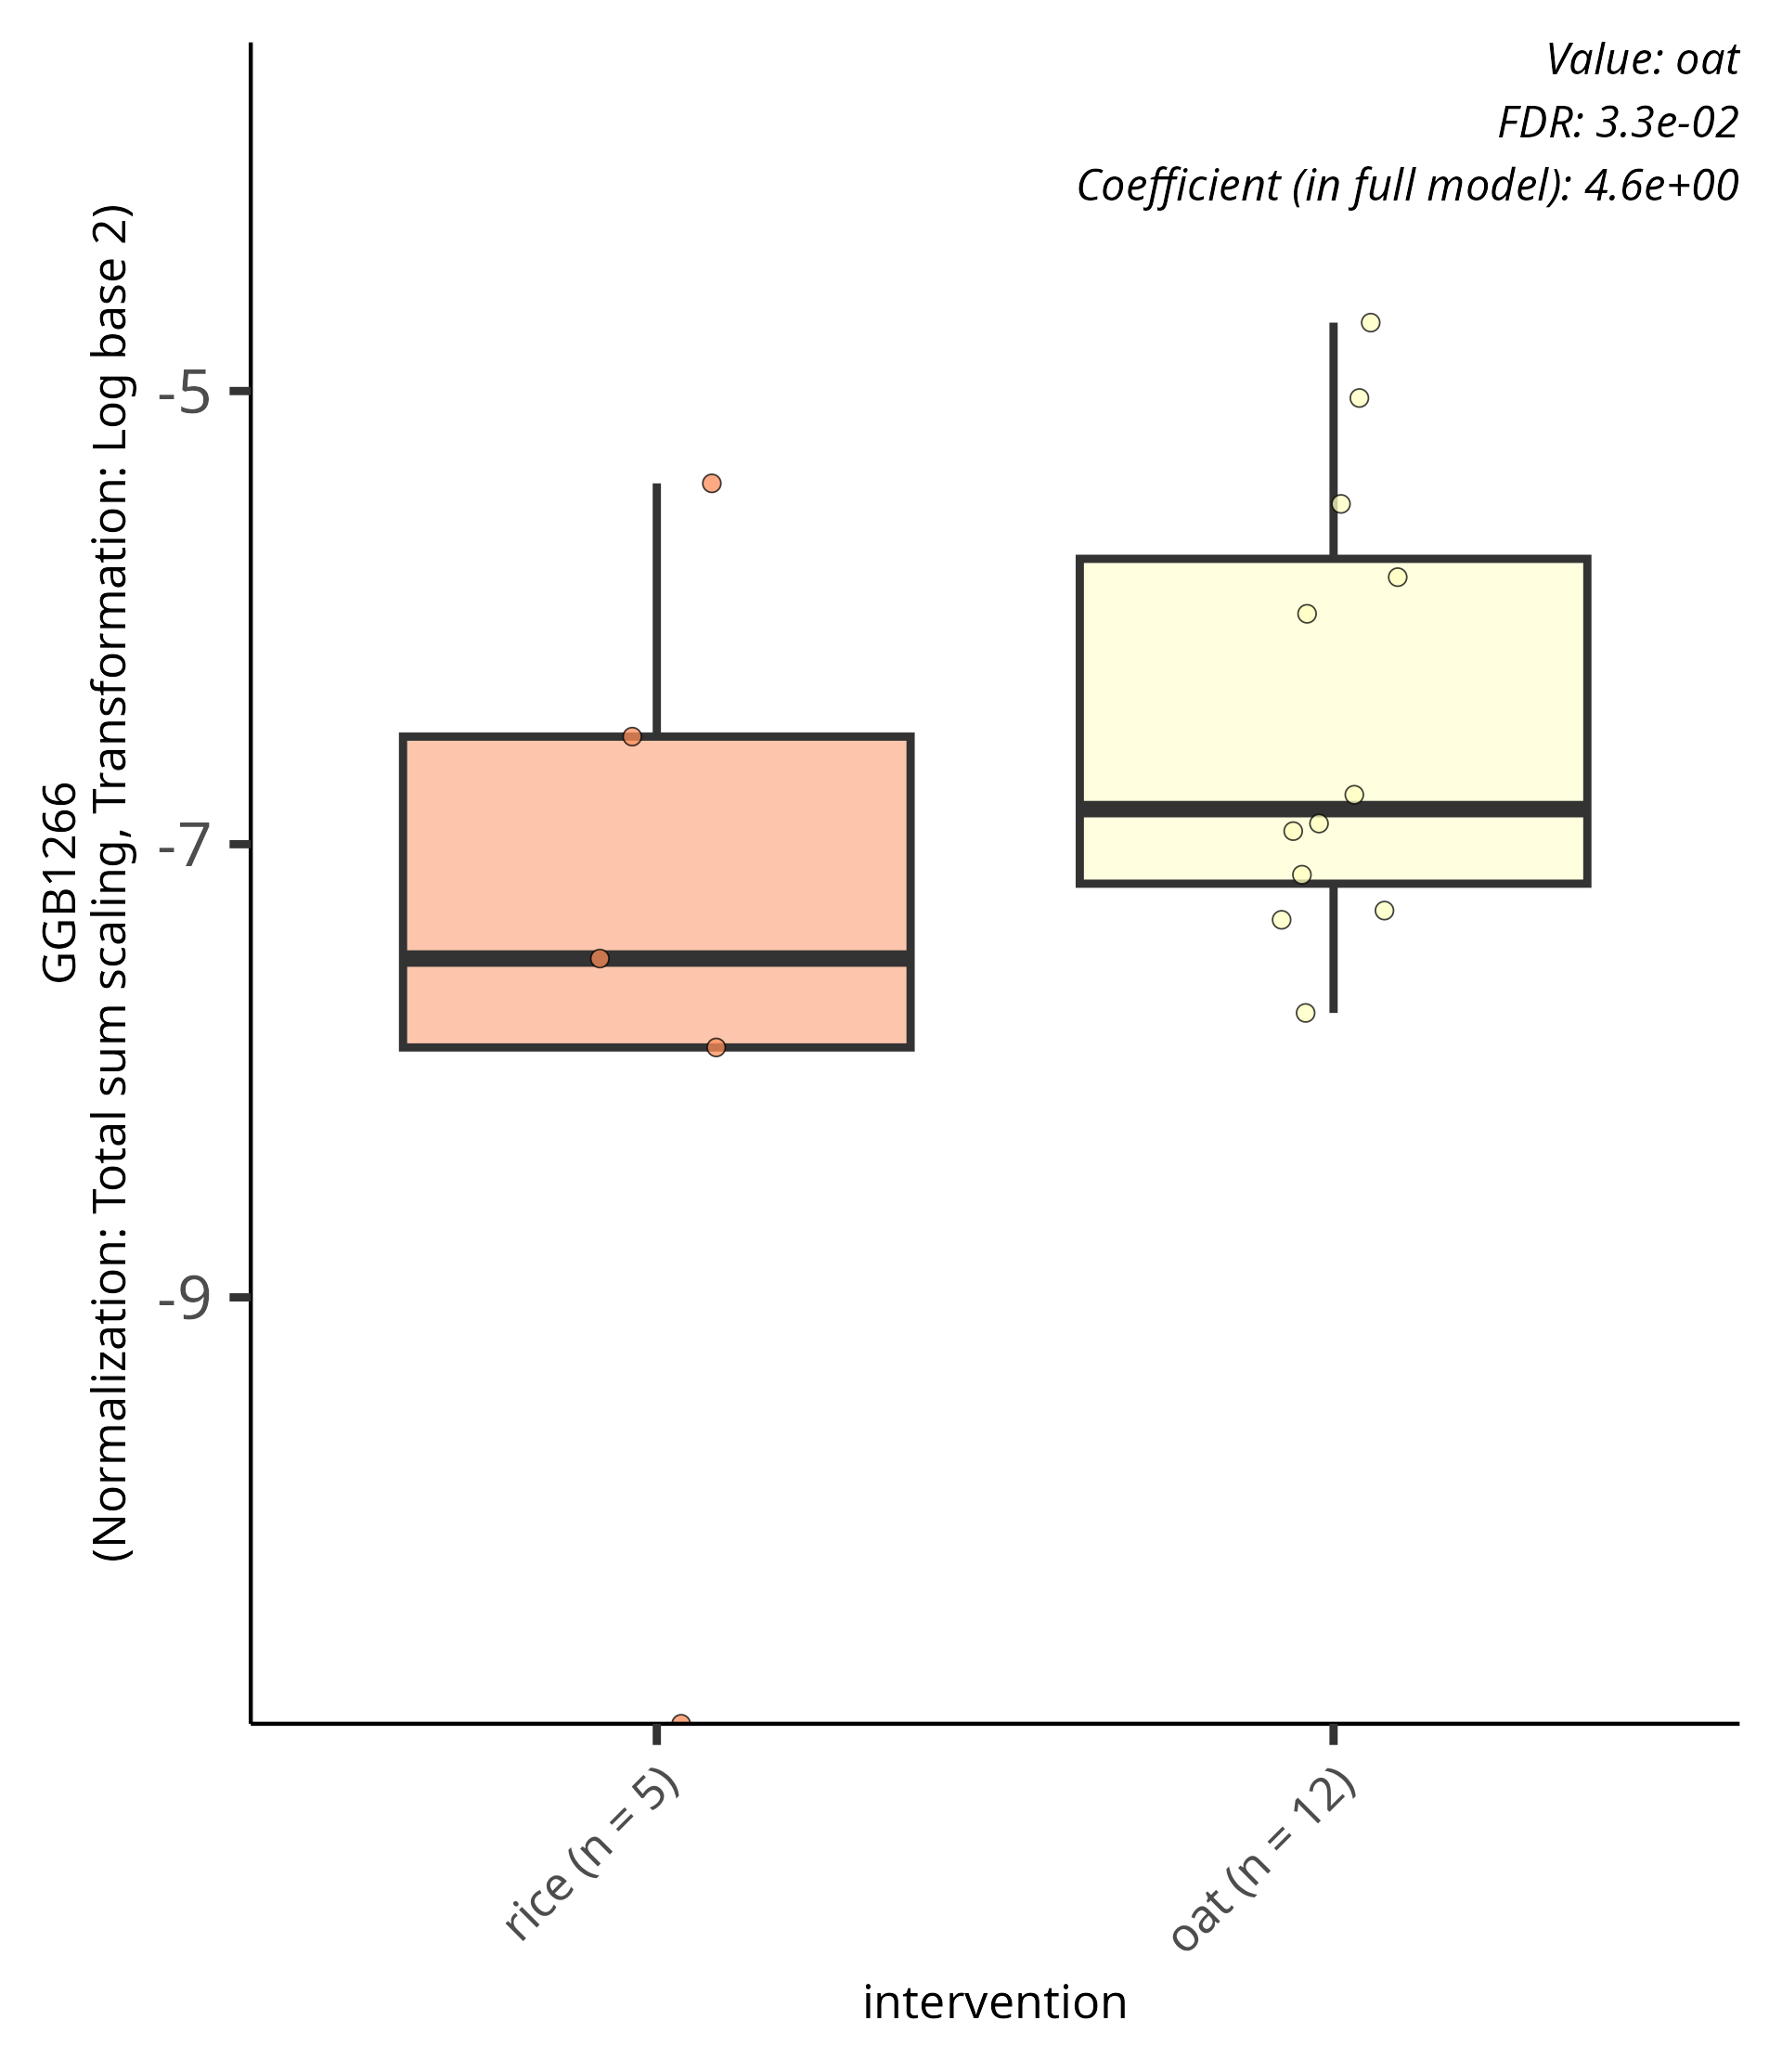
\includegraphics{../../output/daa/daa_taxa/genus/figures/association_plots/intervention/linear/intervention_GGB1266_linear.png}\\
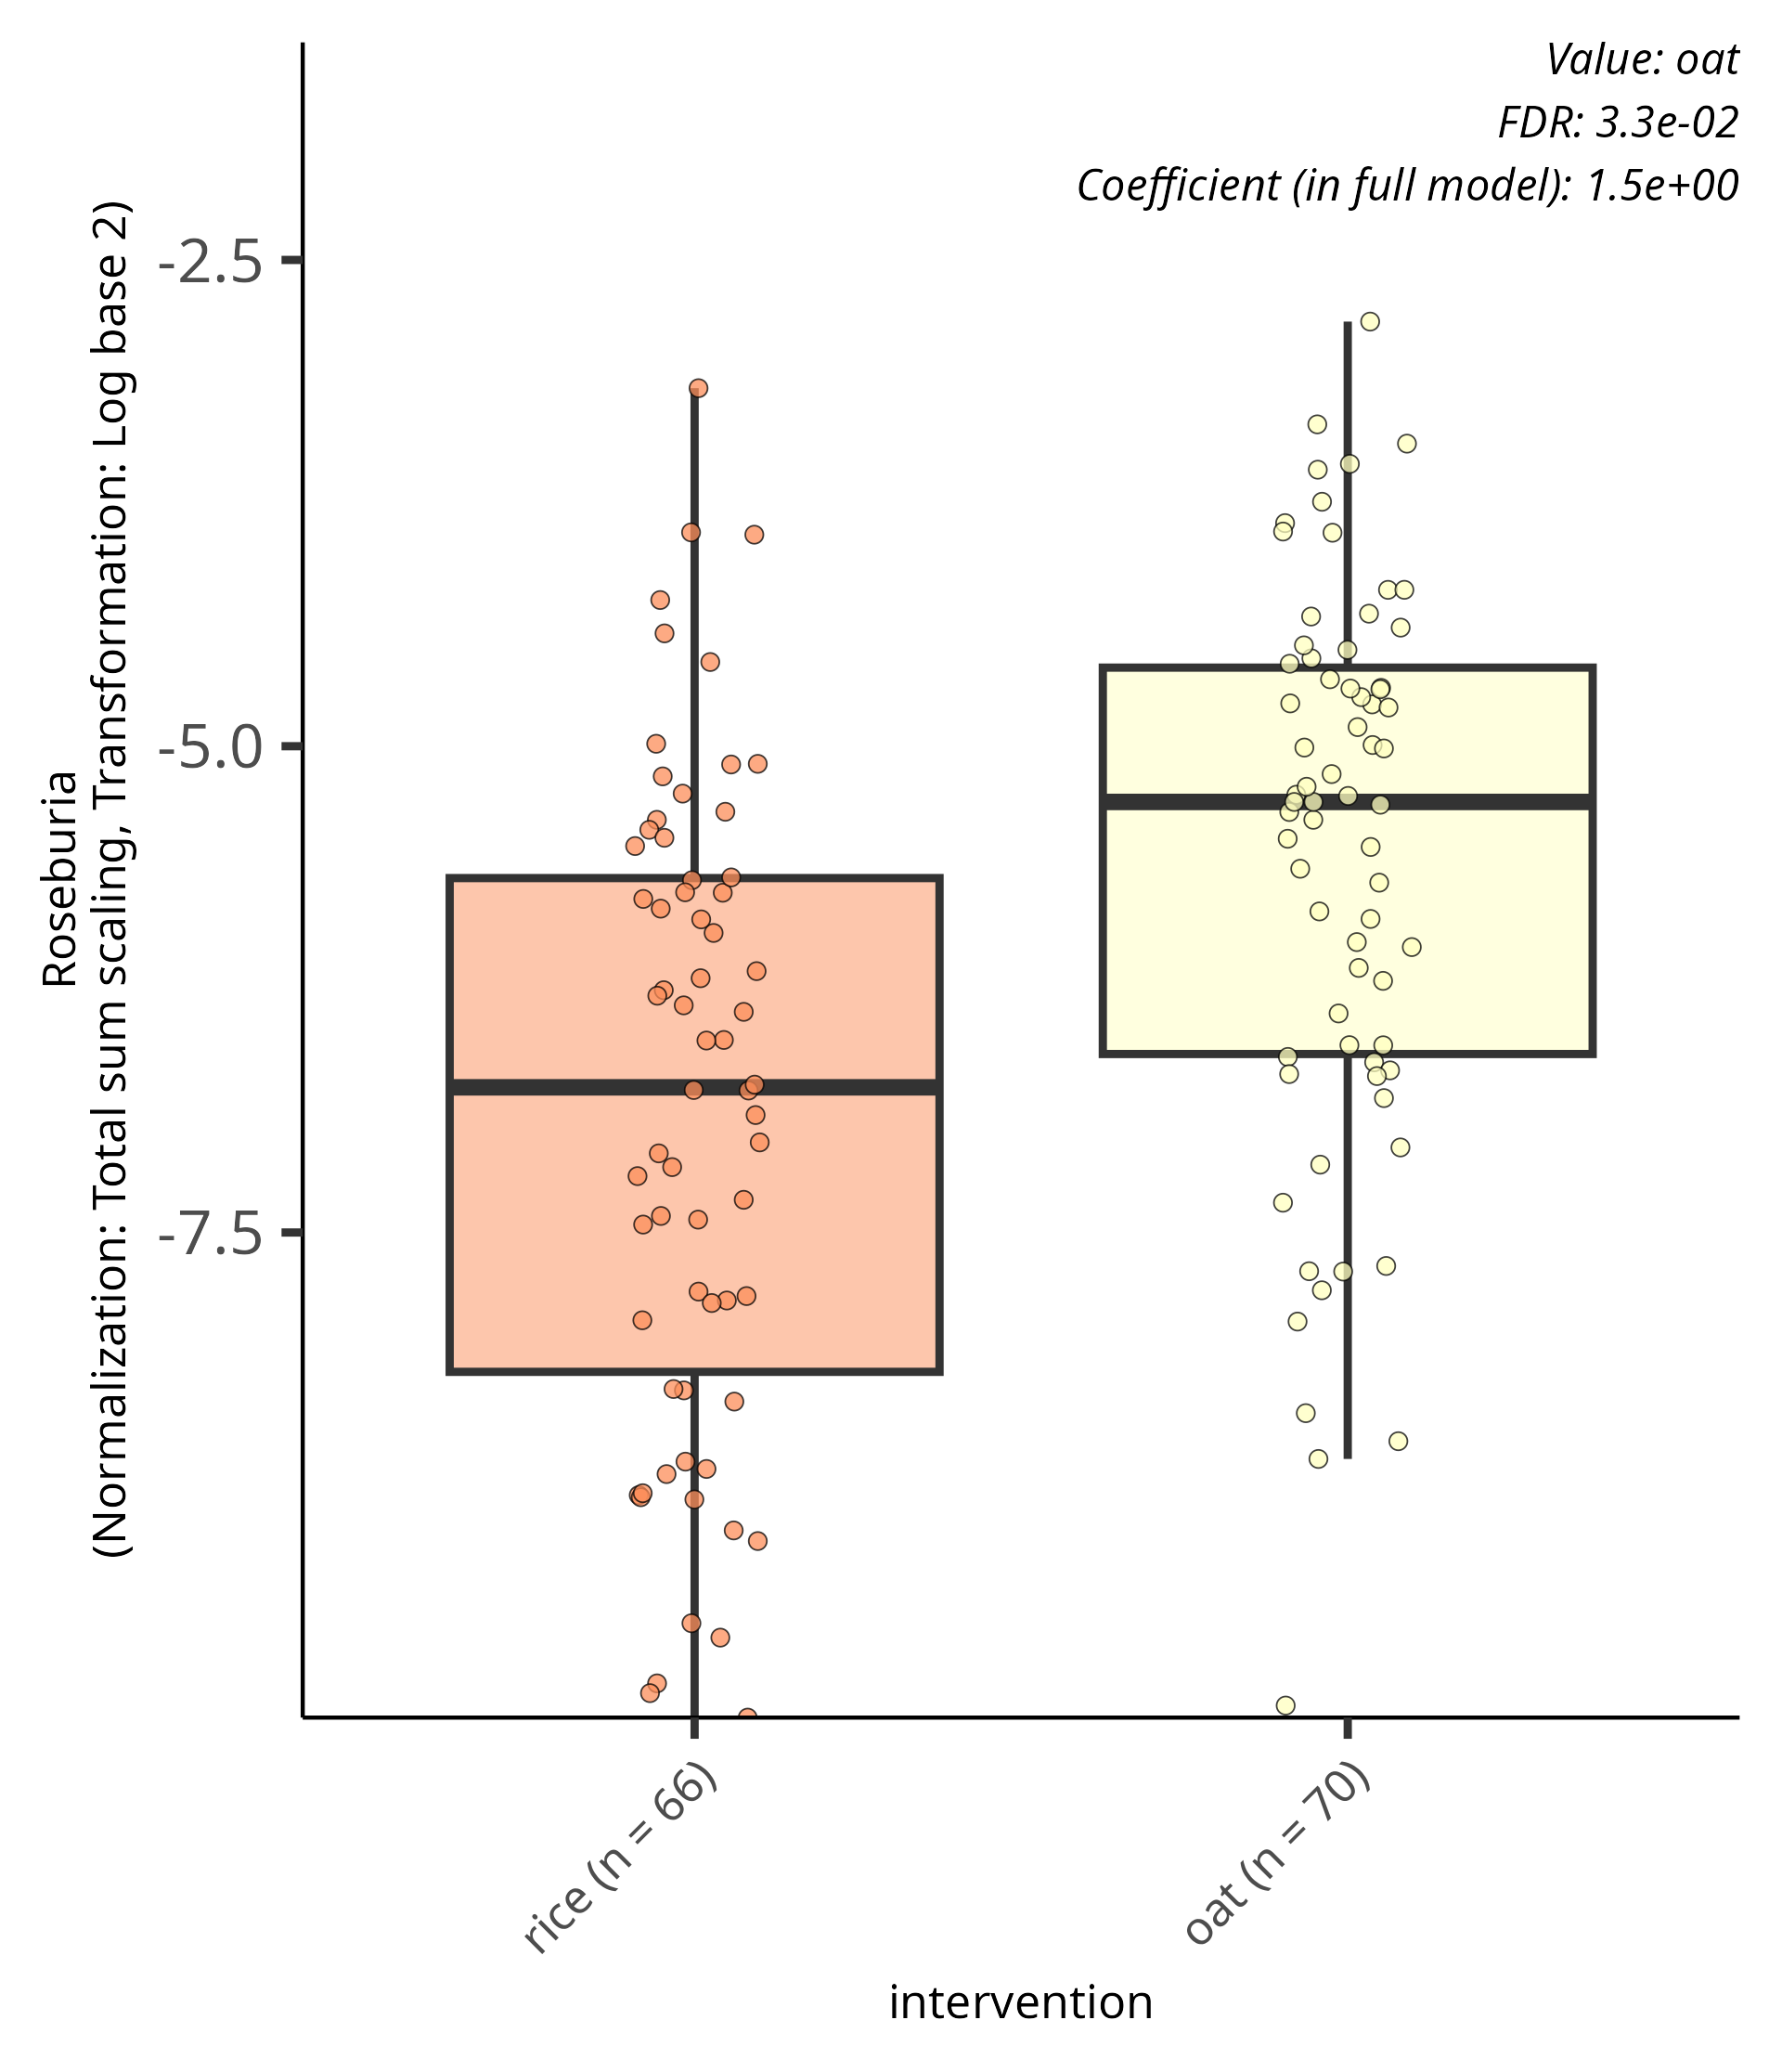
\includegraphics{../../output/daa/daa_taxa/genus/figures/association_plots/intervention/linear/intervention_Roseburia_linear.png}\\
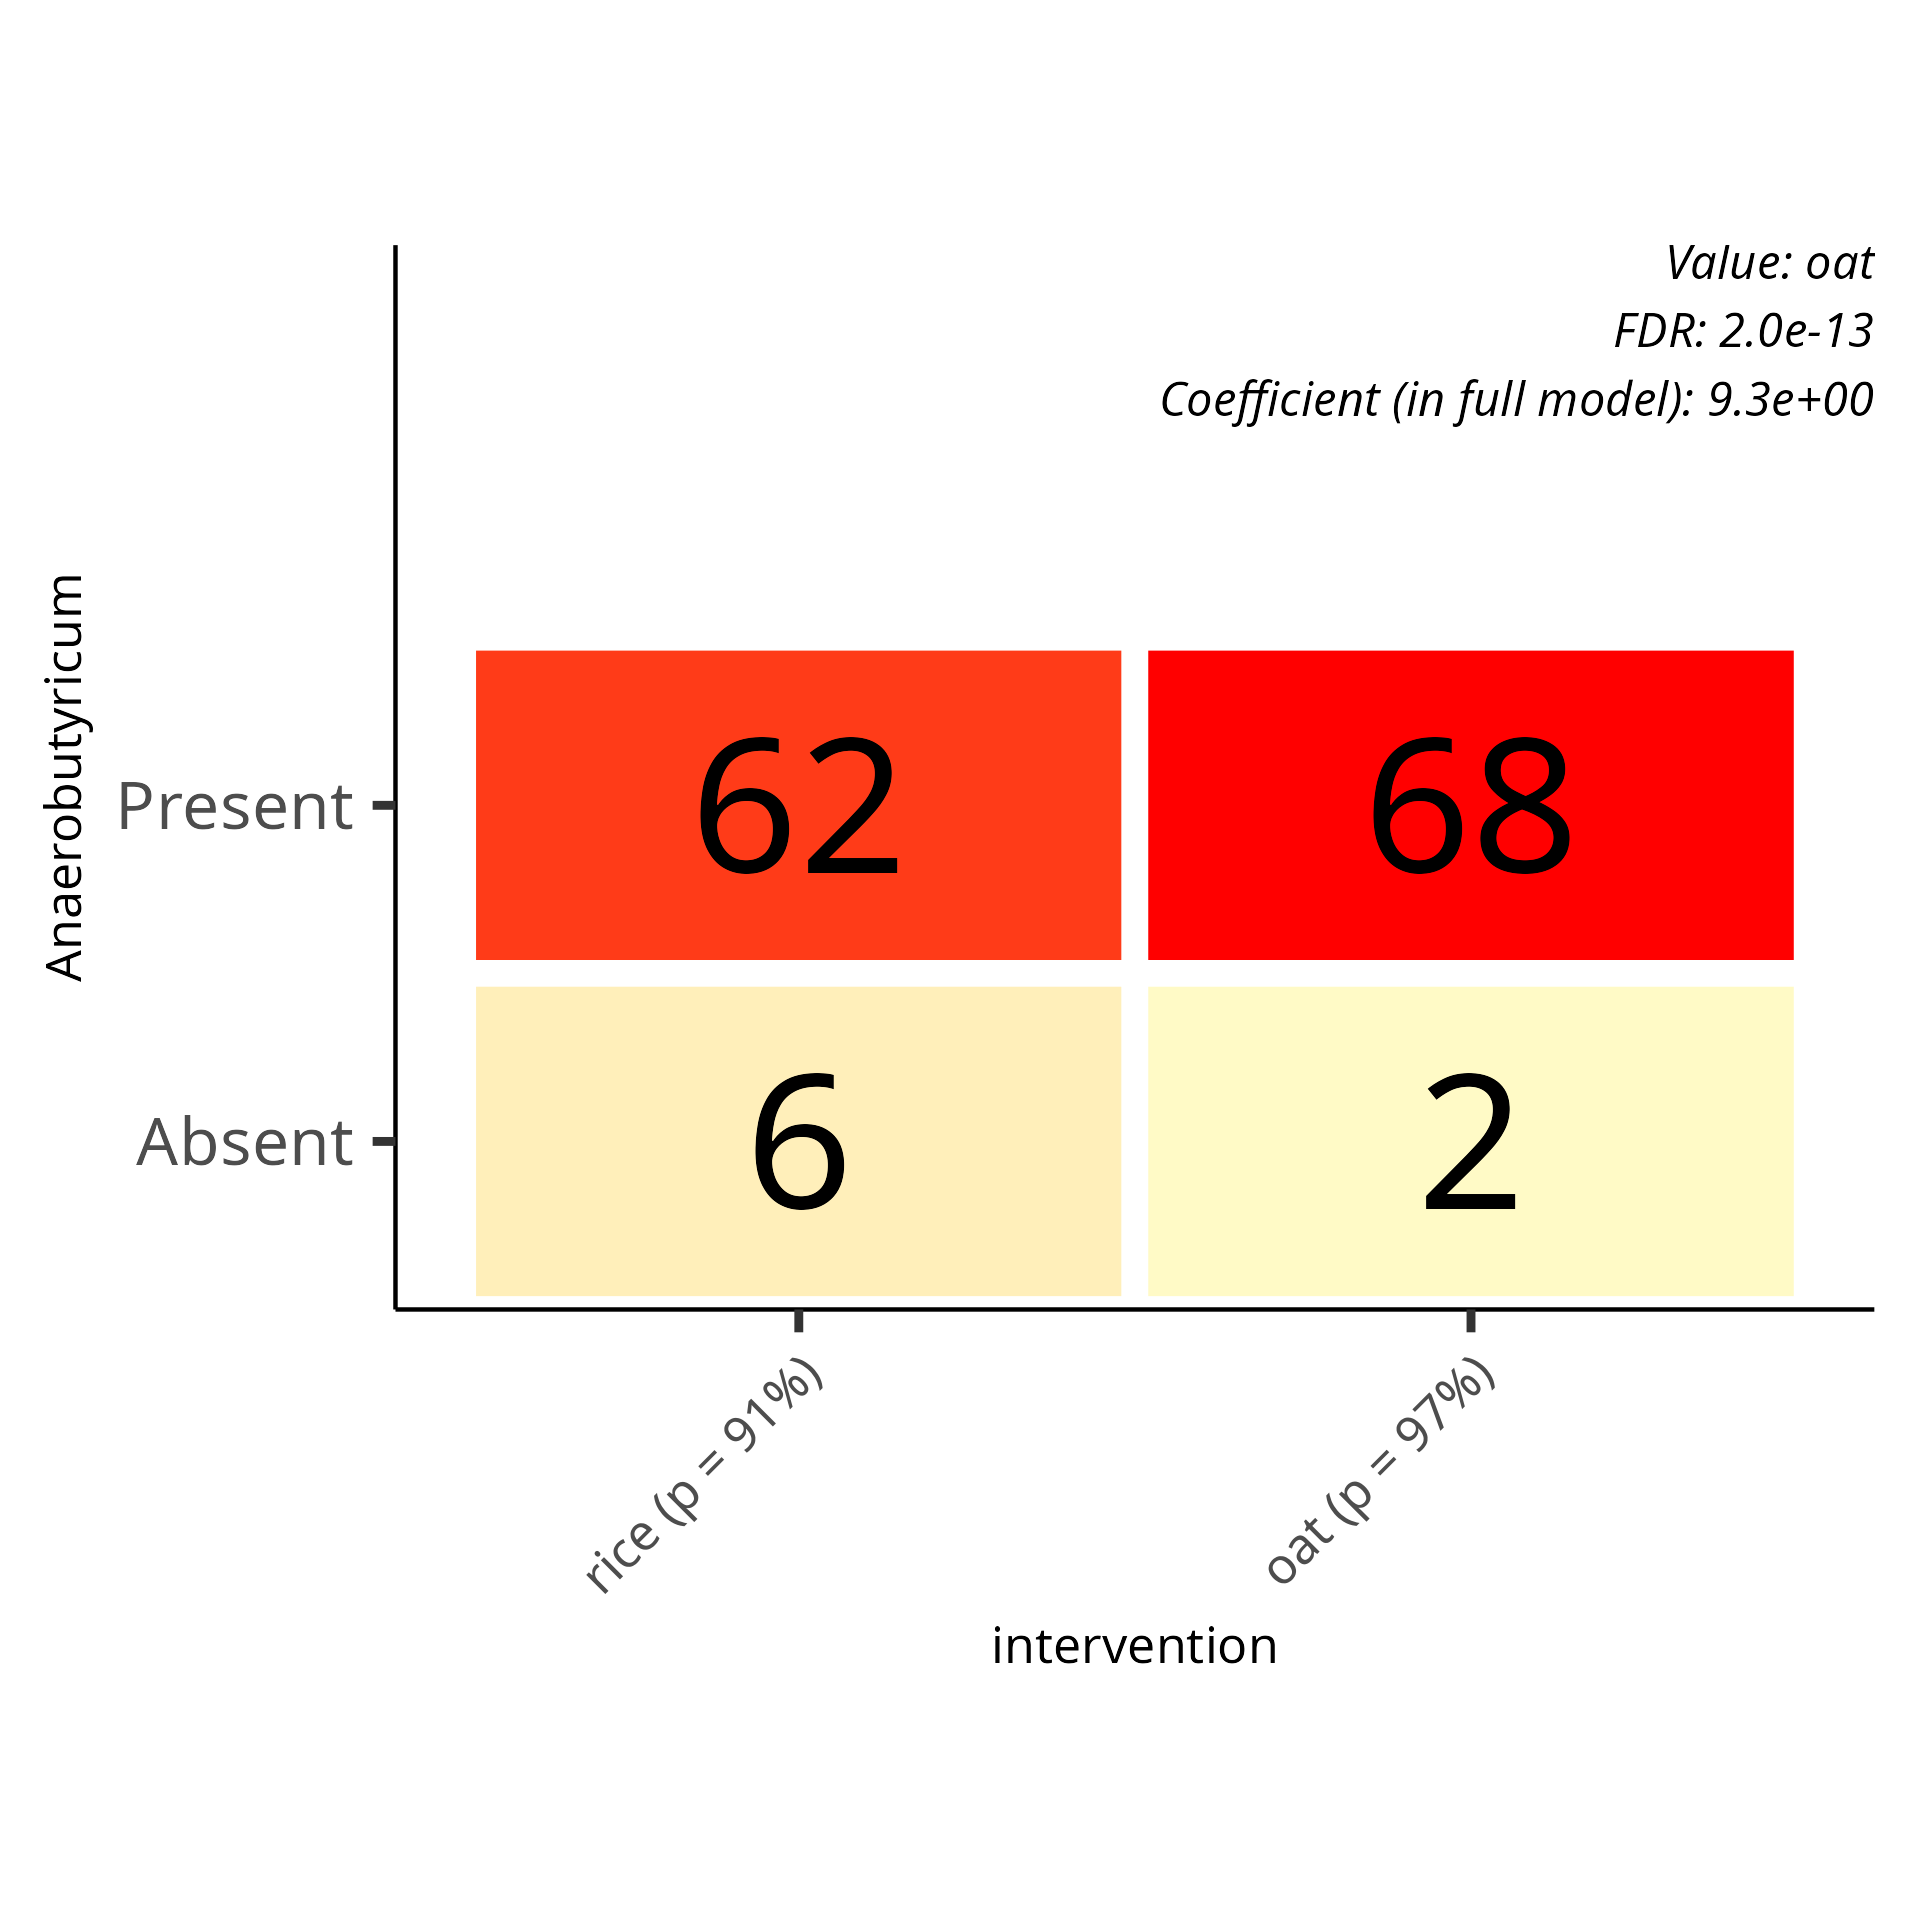
\includegraphics{../../output/daa/daa_taxa/genus/figures/association_plots/intervention/logistic/intervention_Anaerobutyricum_logistic.png}\\
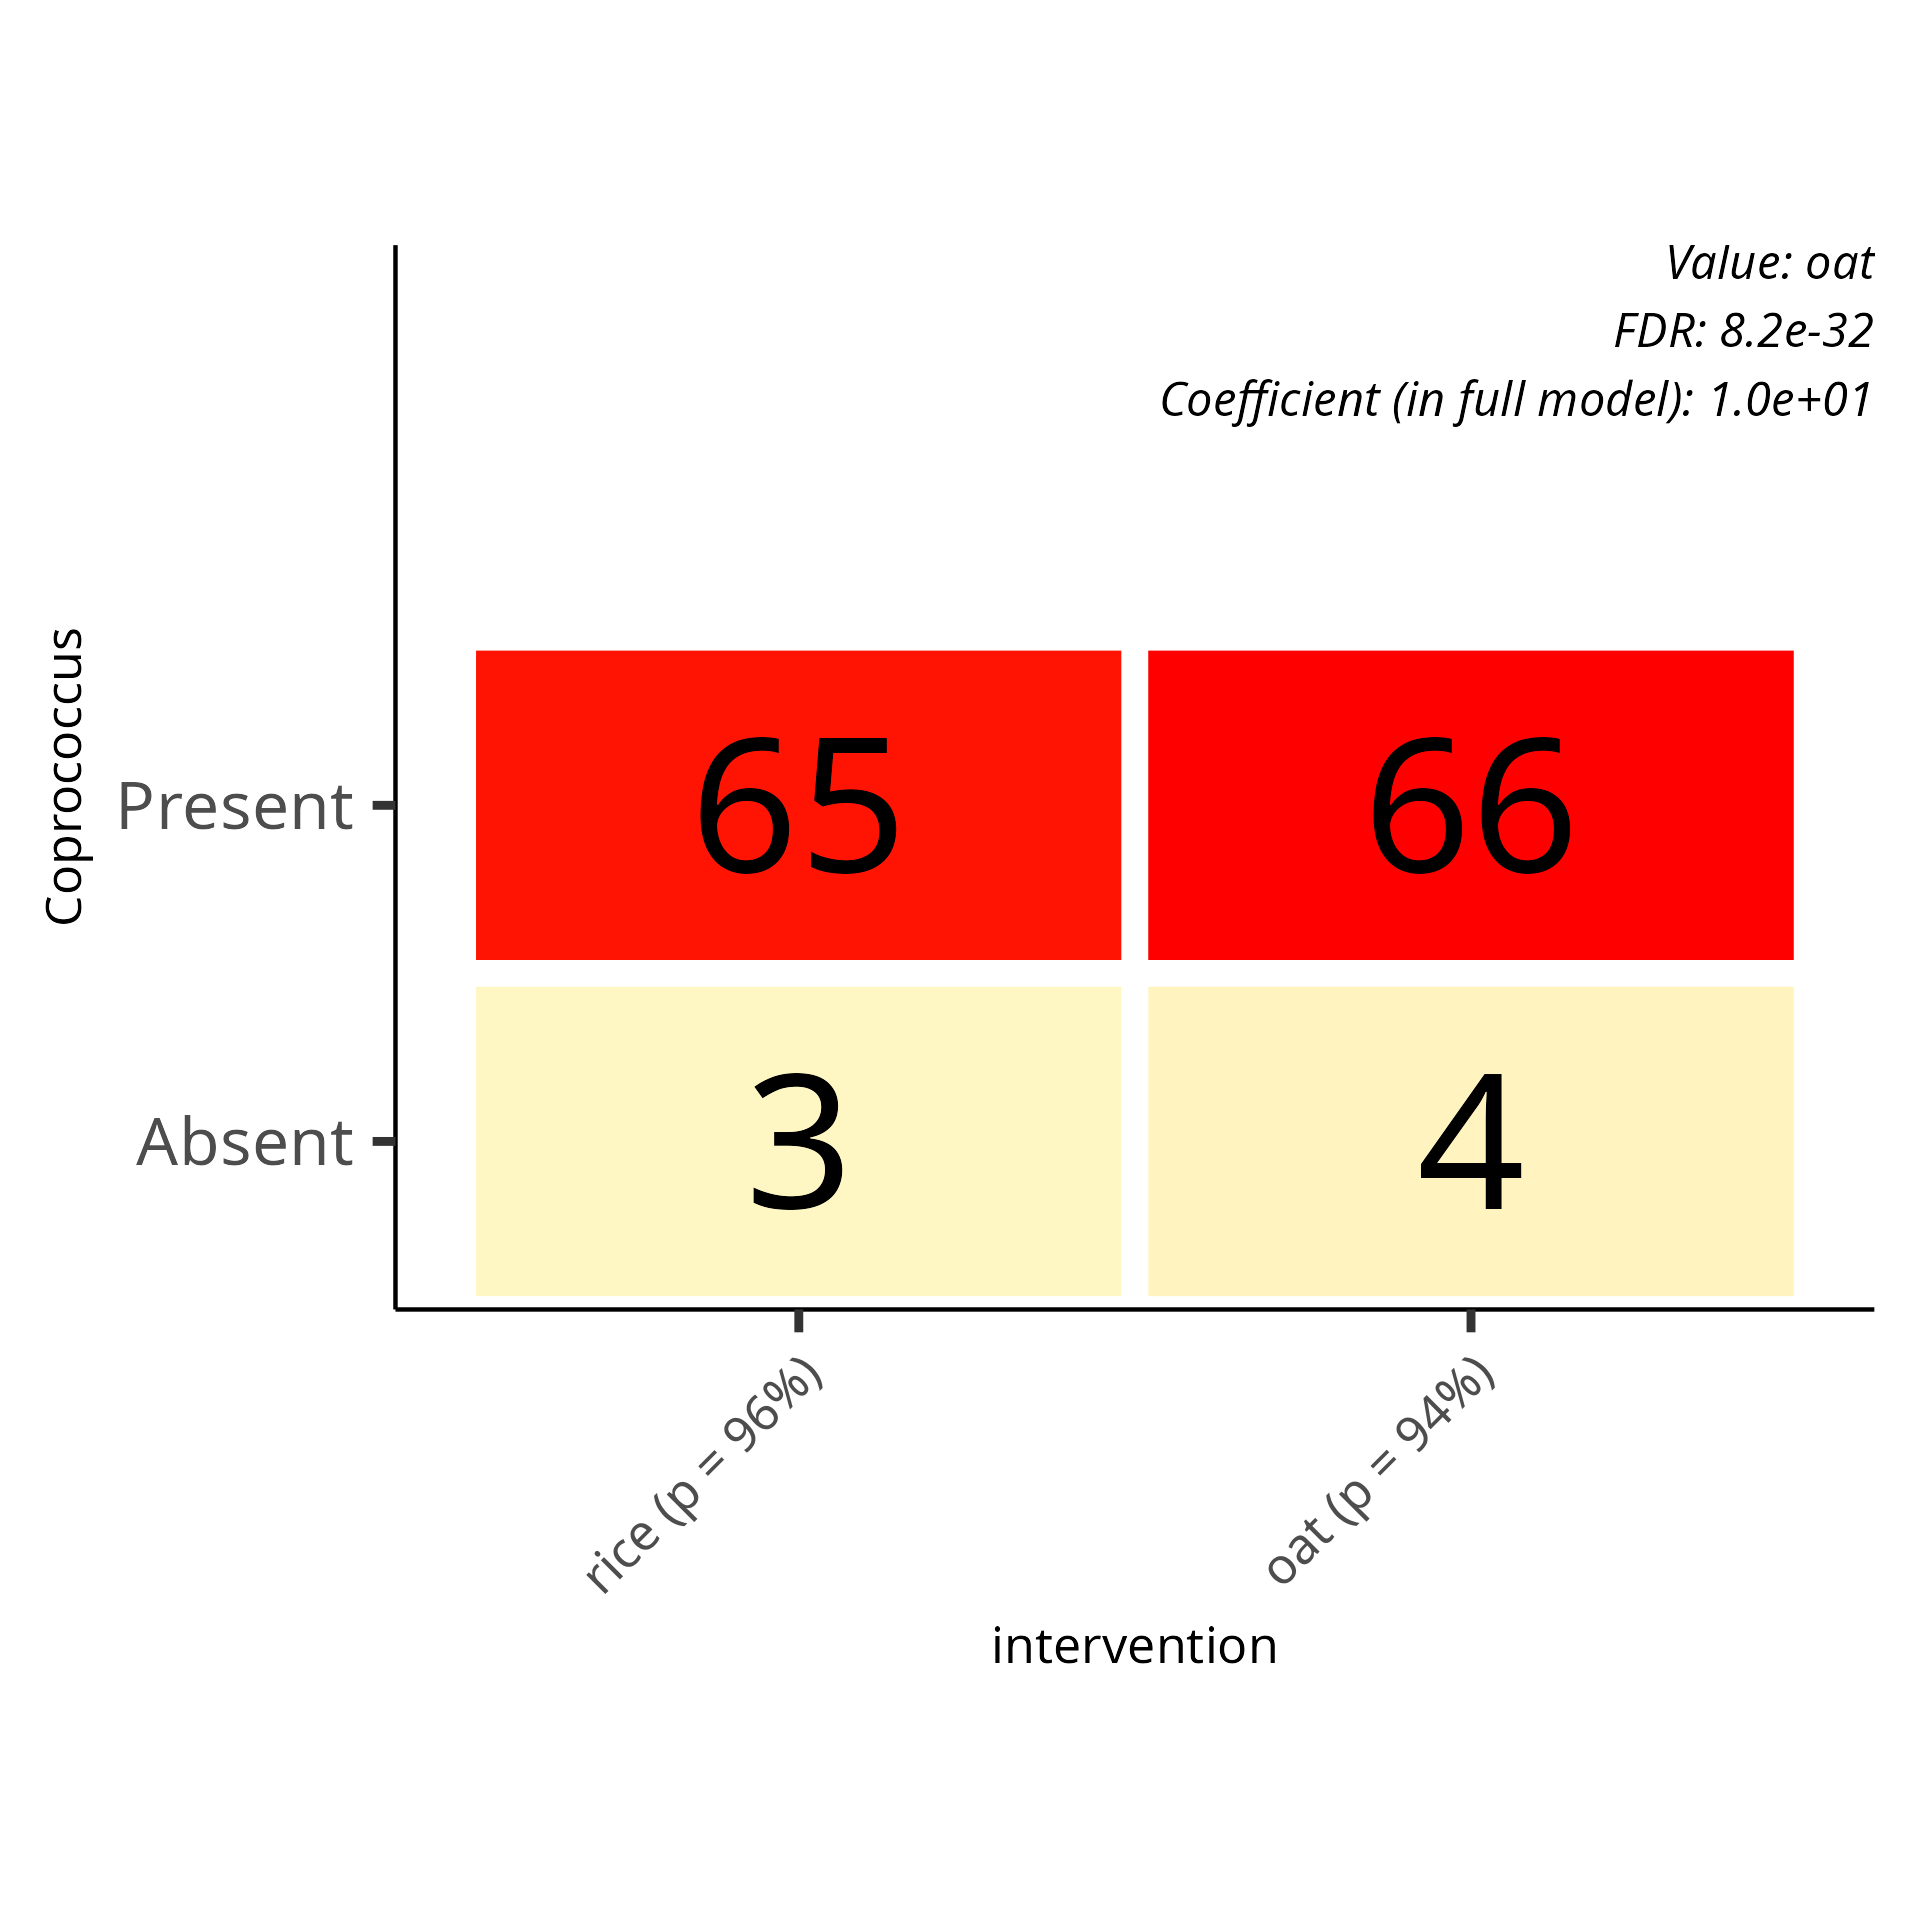
\includegraphics{../../output/daa/daa_taxa/genus/figures/association_plots/intervention/logistic/intervention_Coprococcus_logistic.png}\\
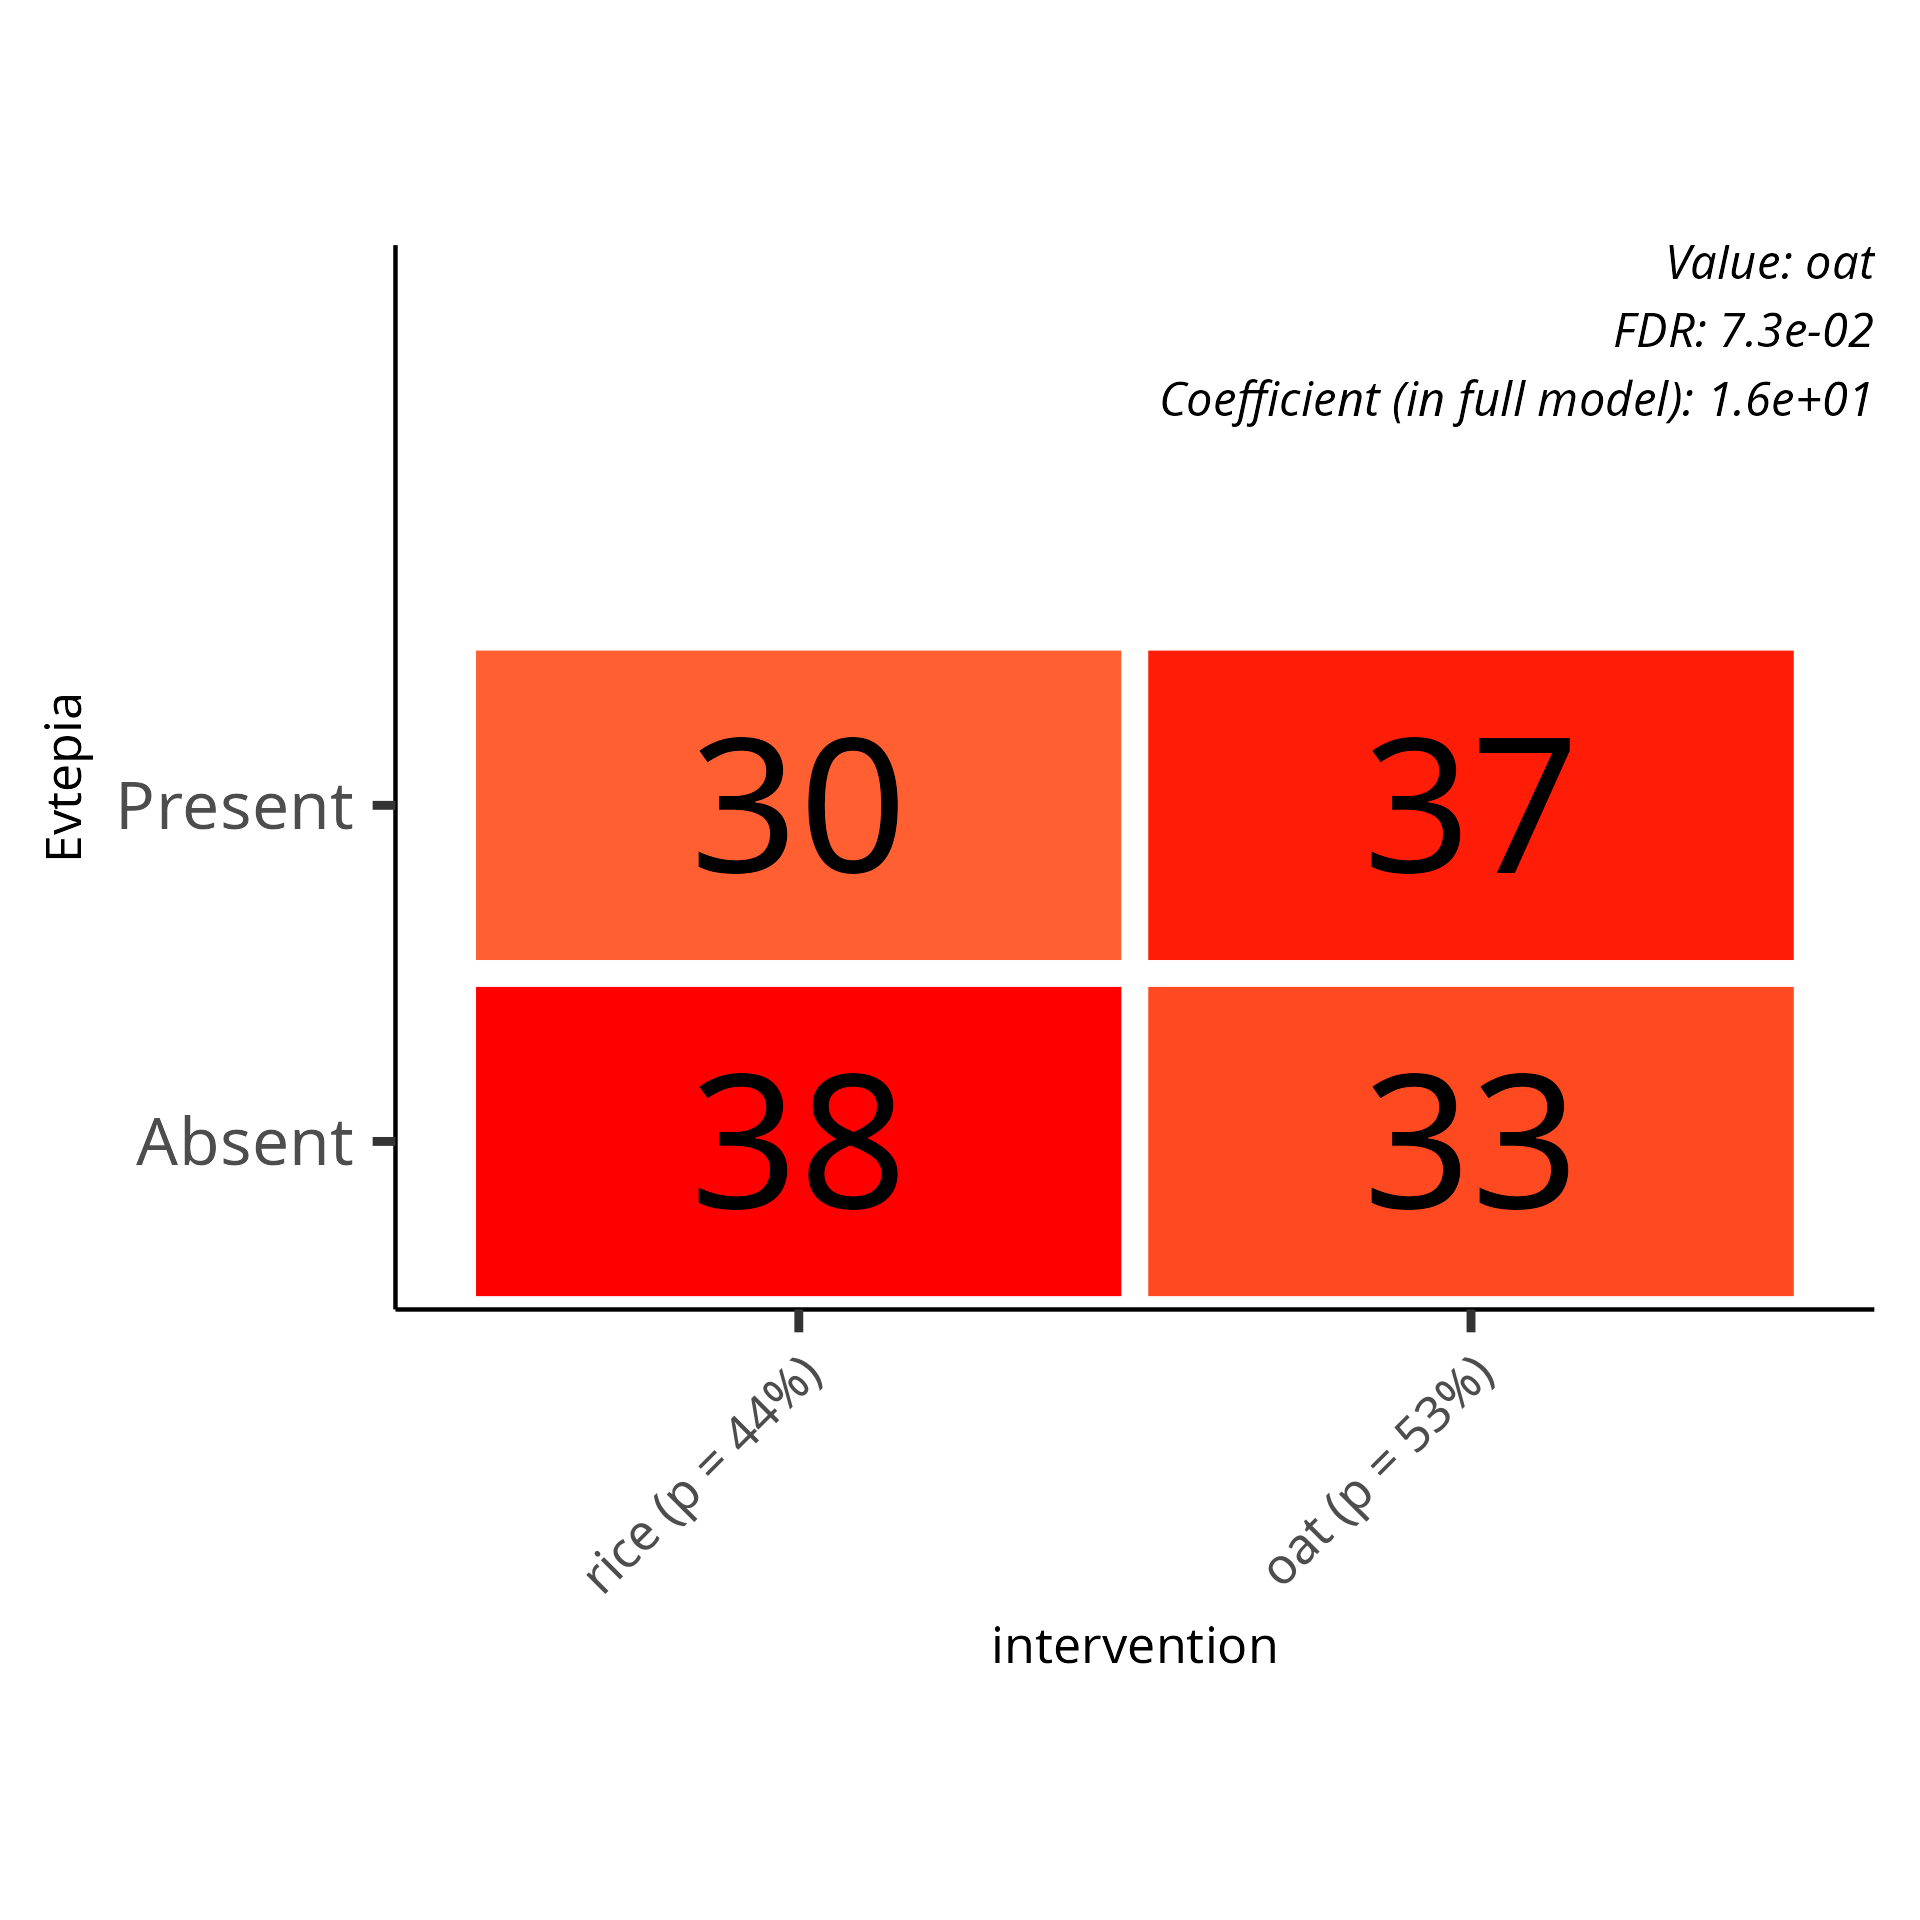
\includegraphics{../../output/daa/daa_taxa/genus/figures/association_plots/intervention/logistic/intervention_Evtepia_logistic.png}\\
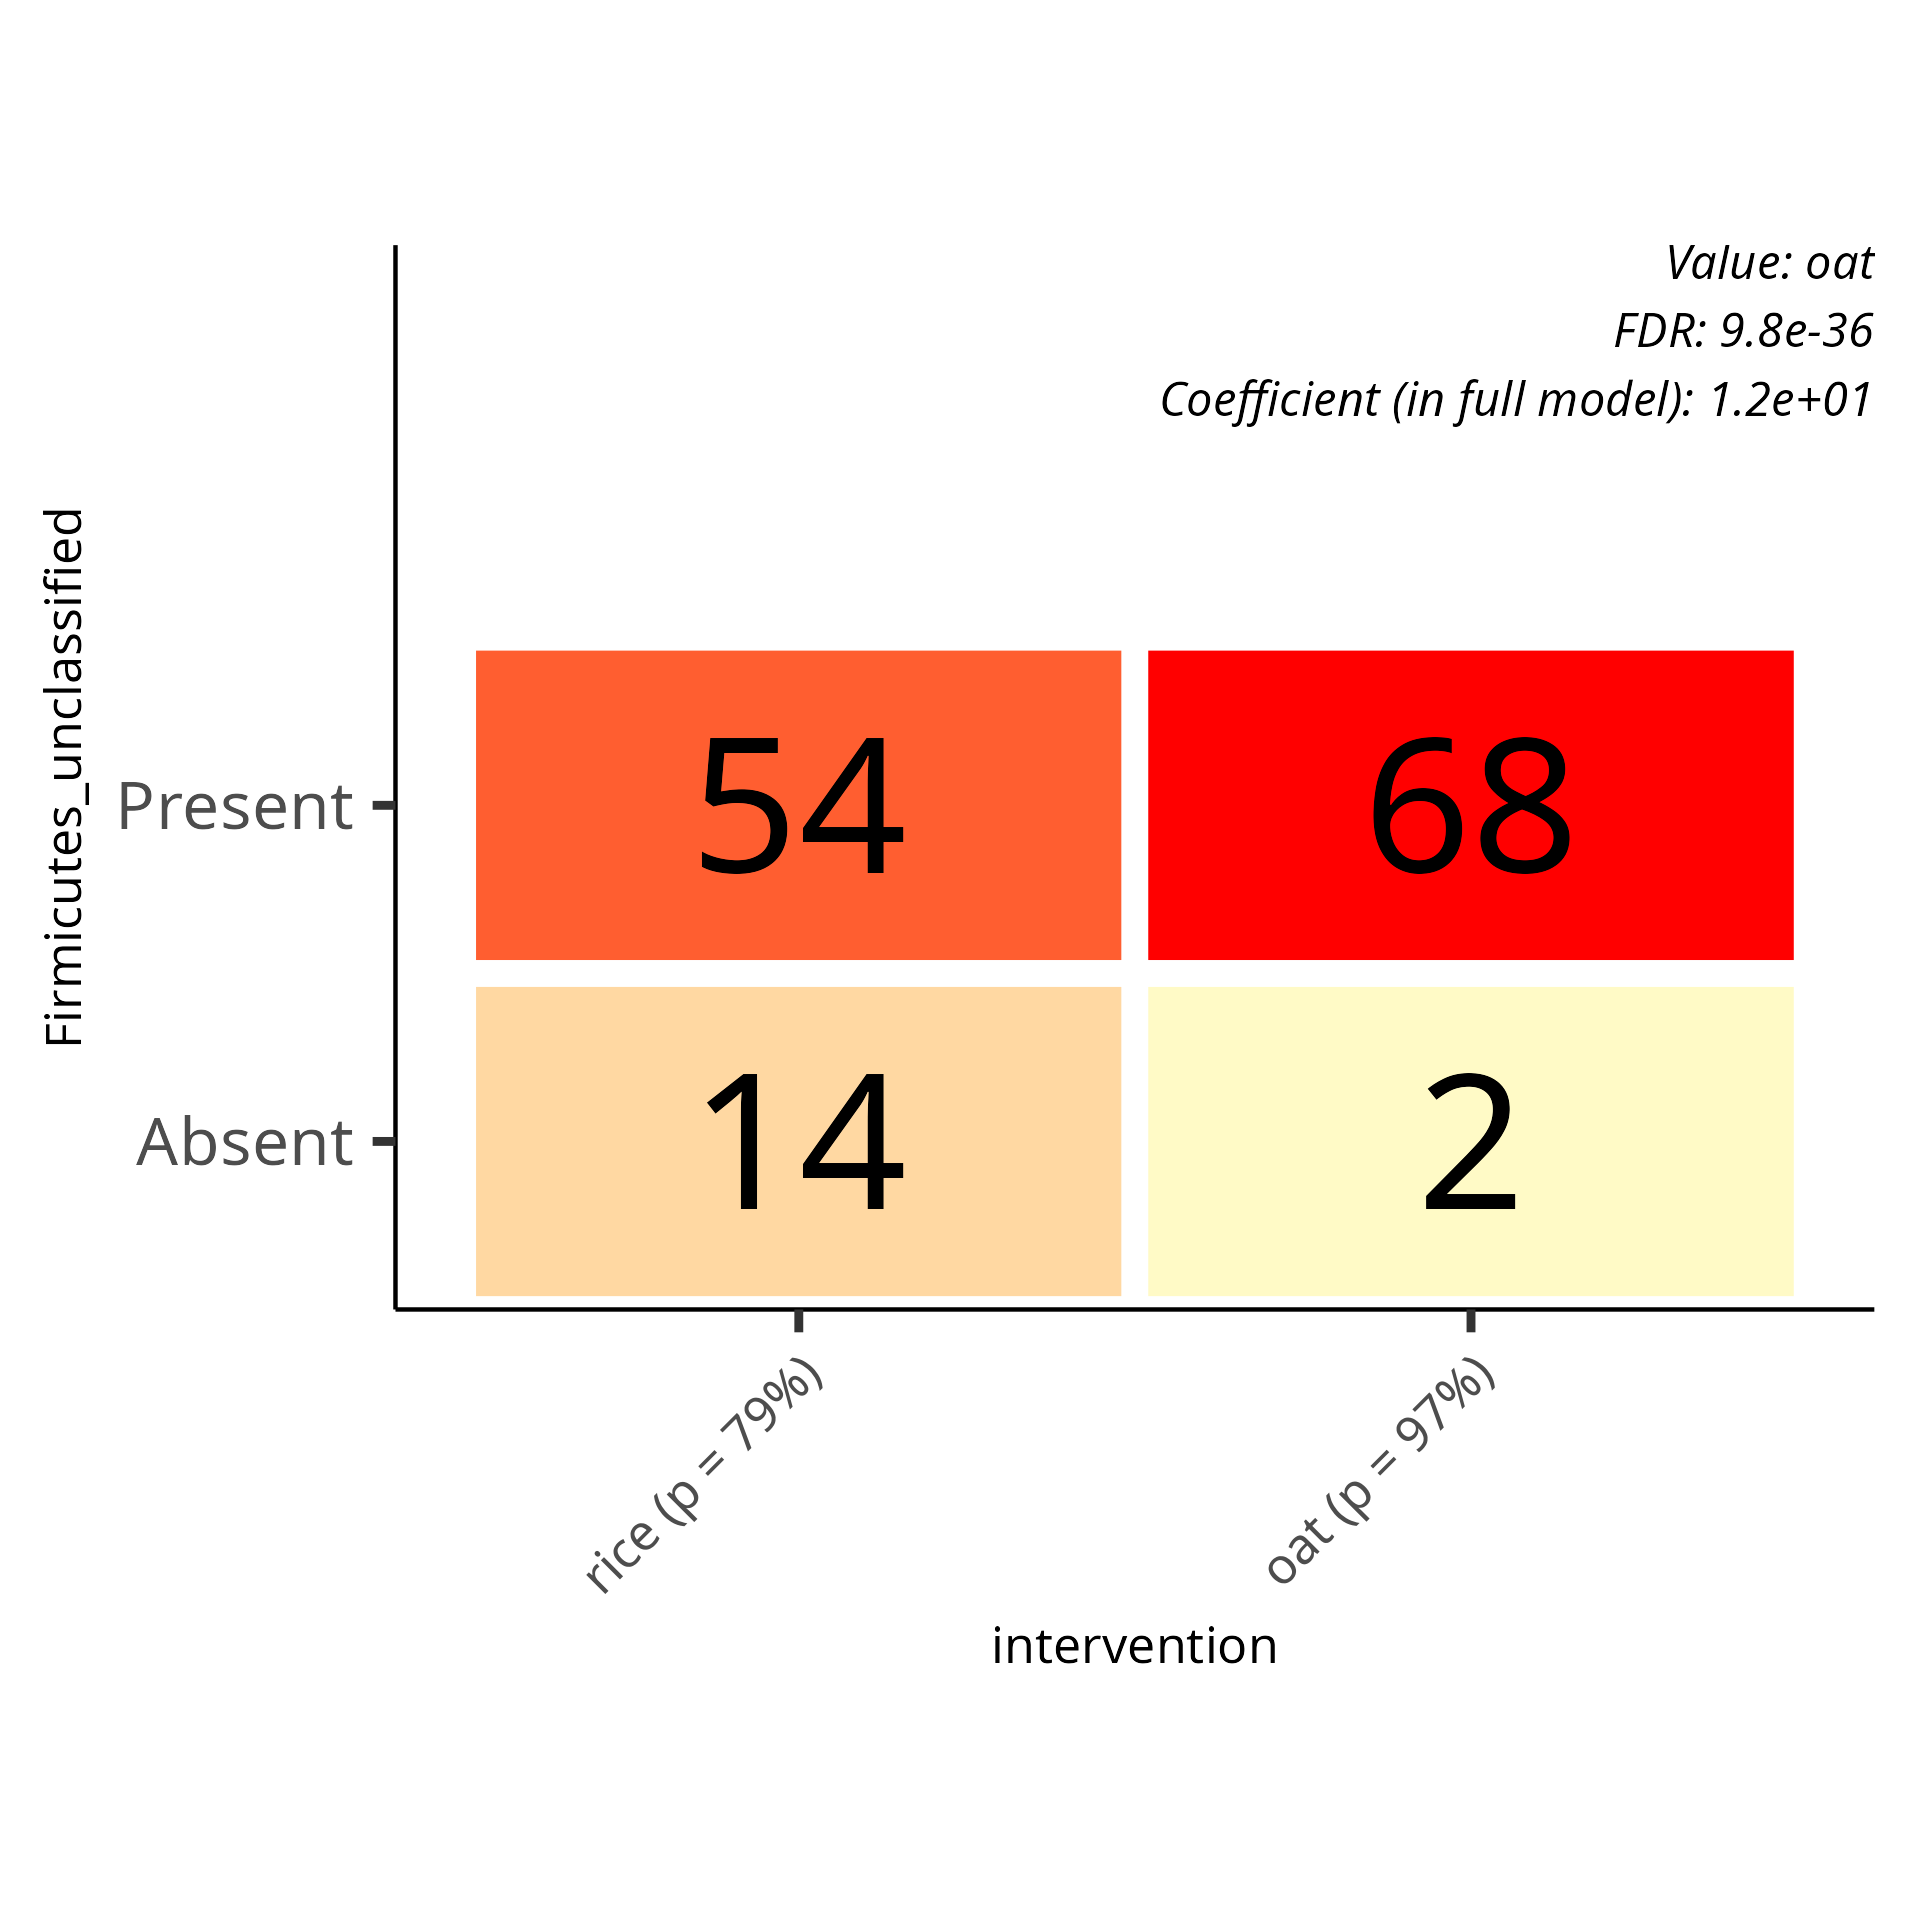
\includegraphics{../../output/daa/daa_taxa/genus/figures/association_plots/intervention/logistic/intervention_Firmicutes_unclassified_logistic.png}\\
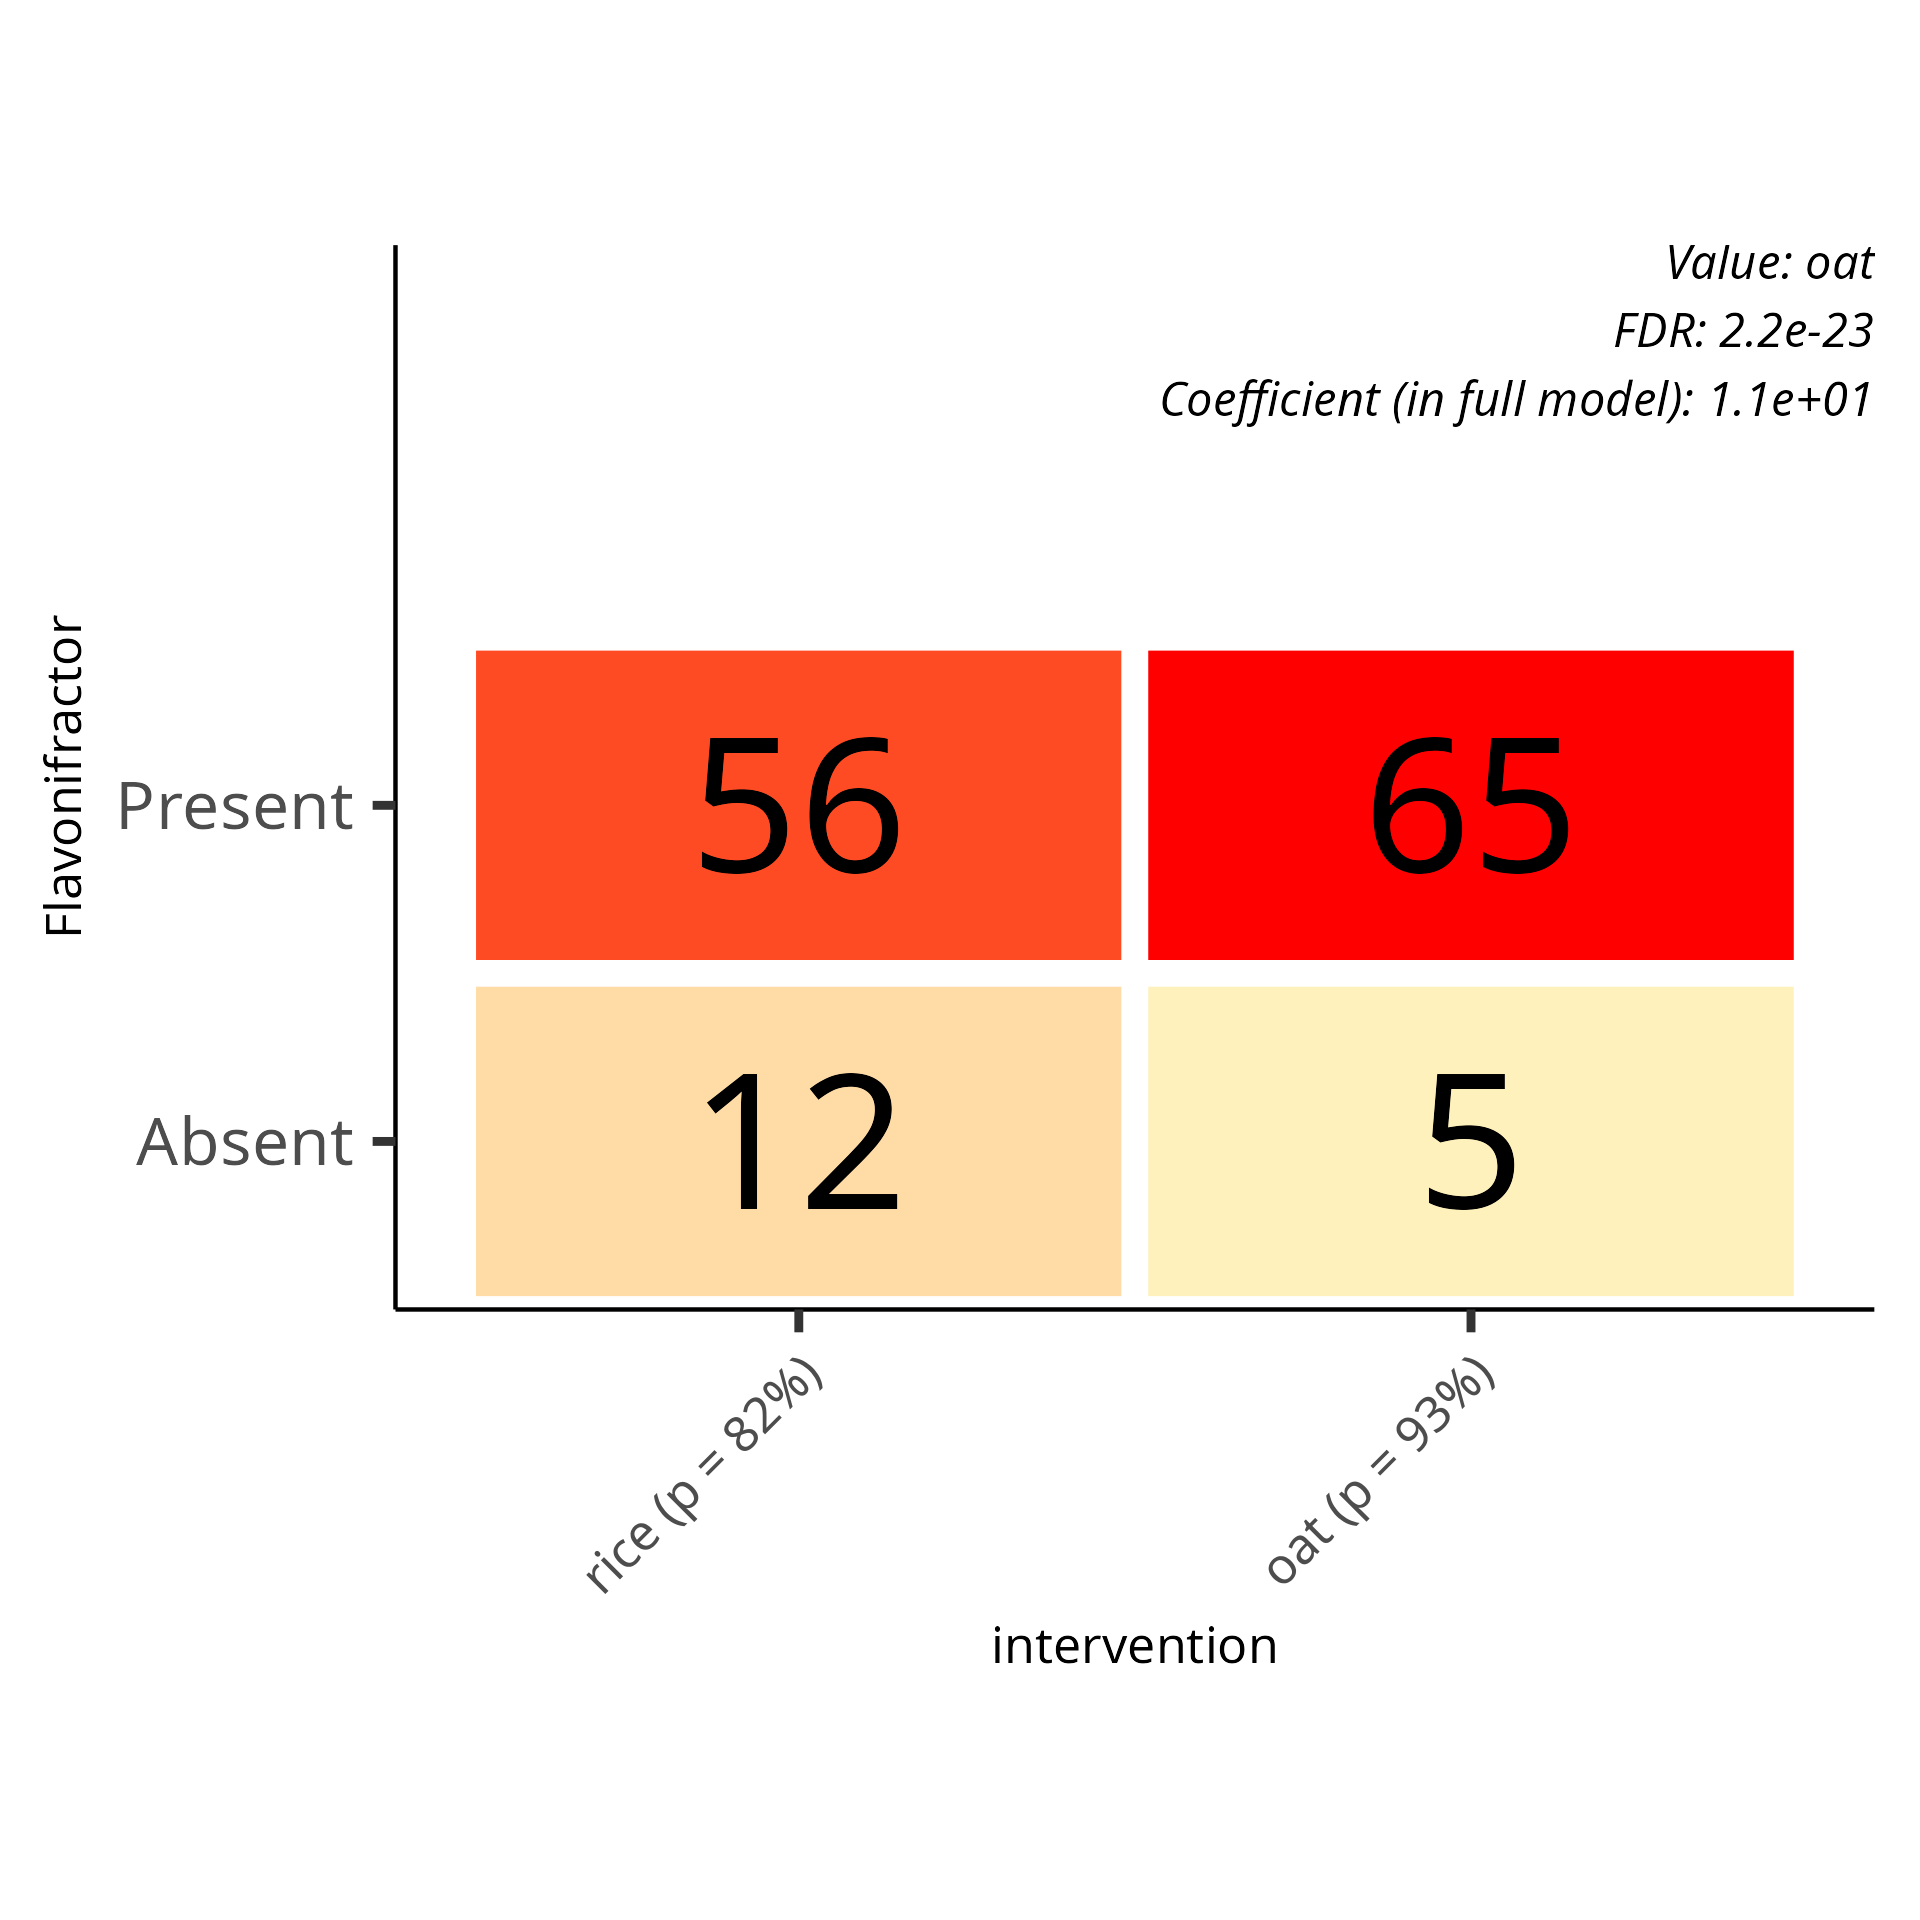
\includegraphics{../../output/daa/daa_taxa/genus/figures/association_plots/intervention/logistic/intervention_Flavonifractor_logistic.png}\\
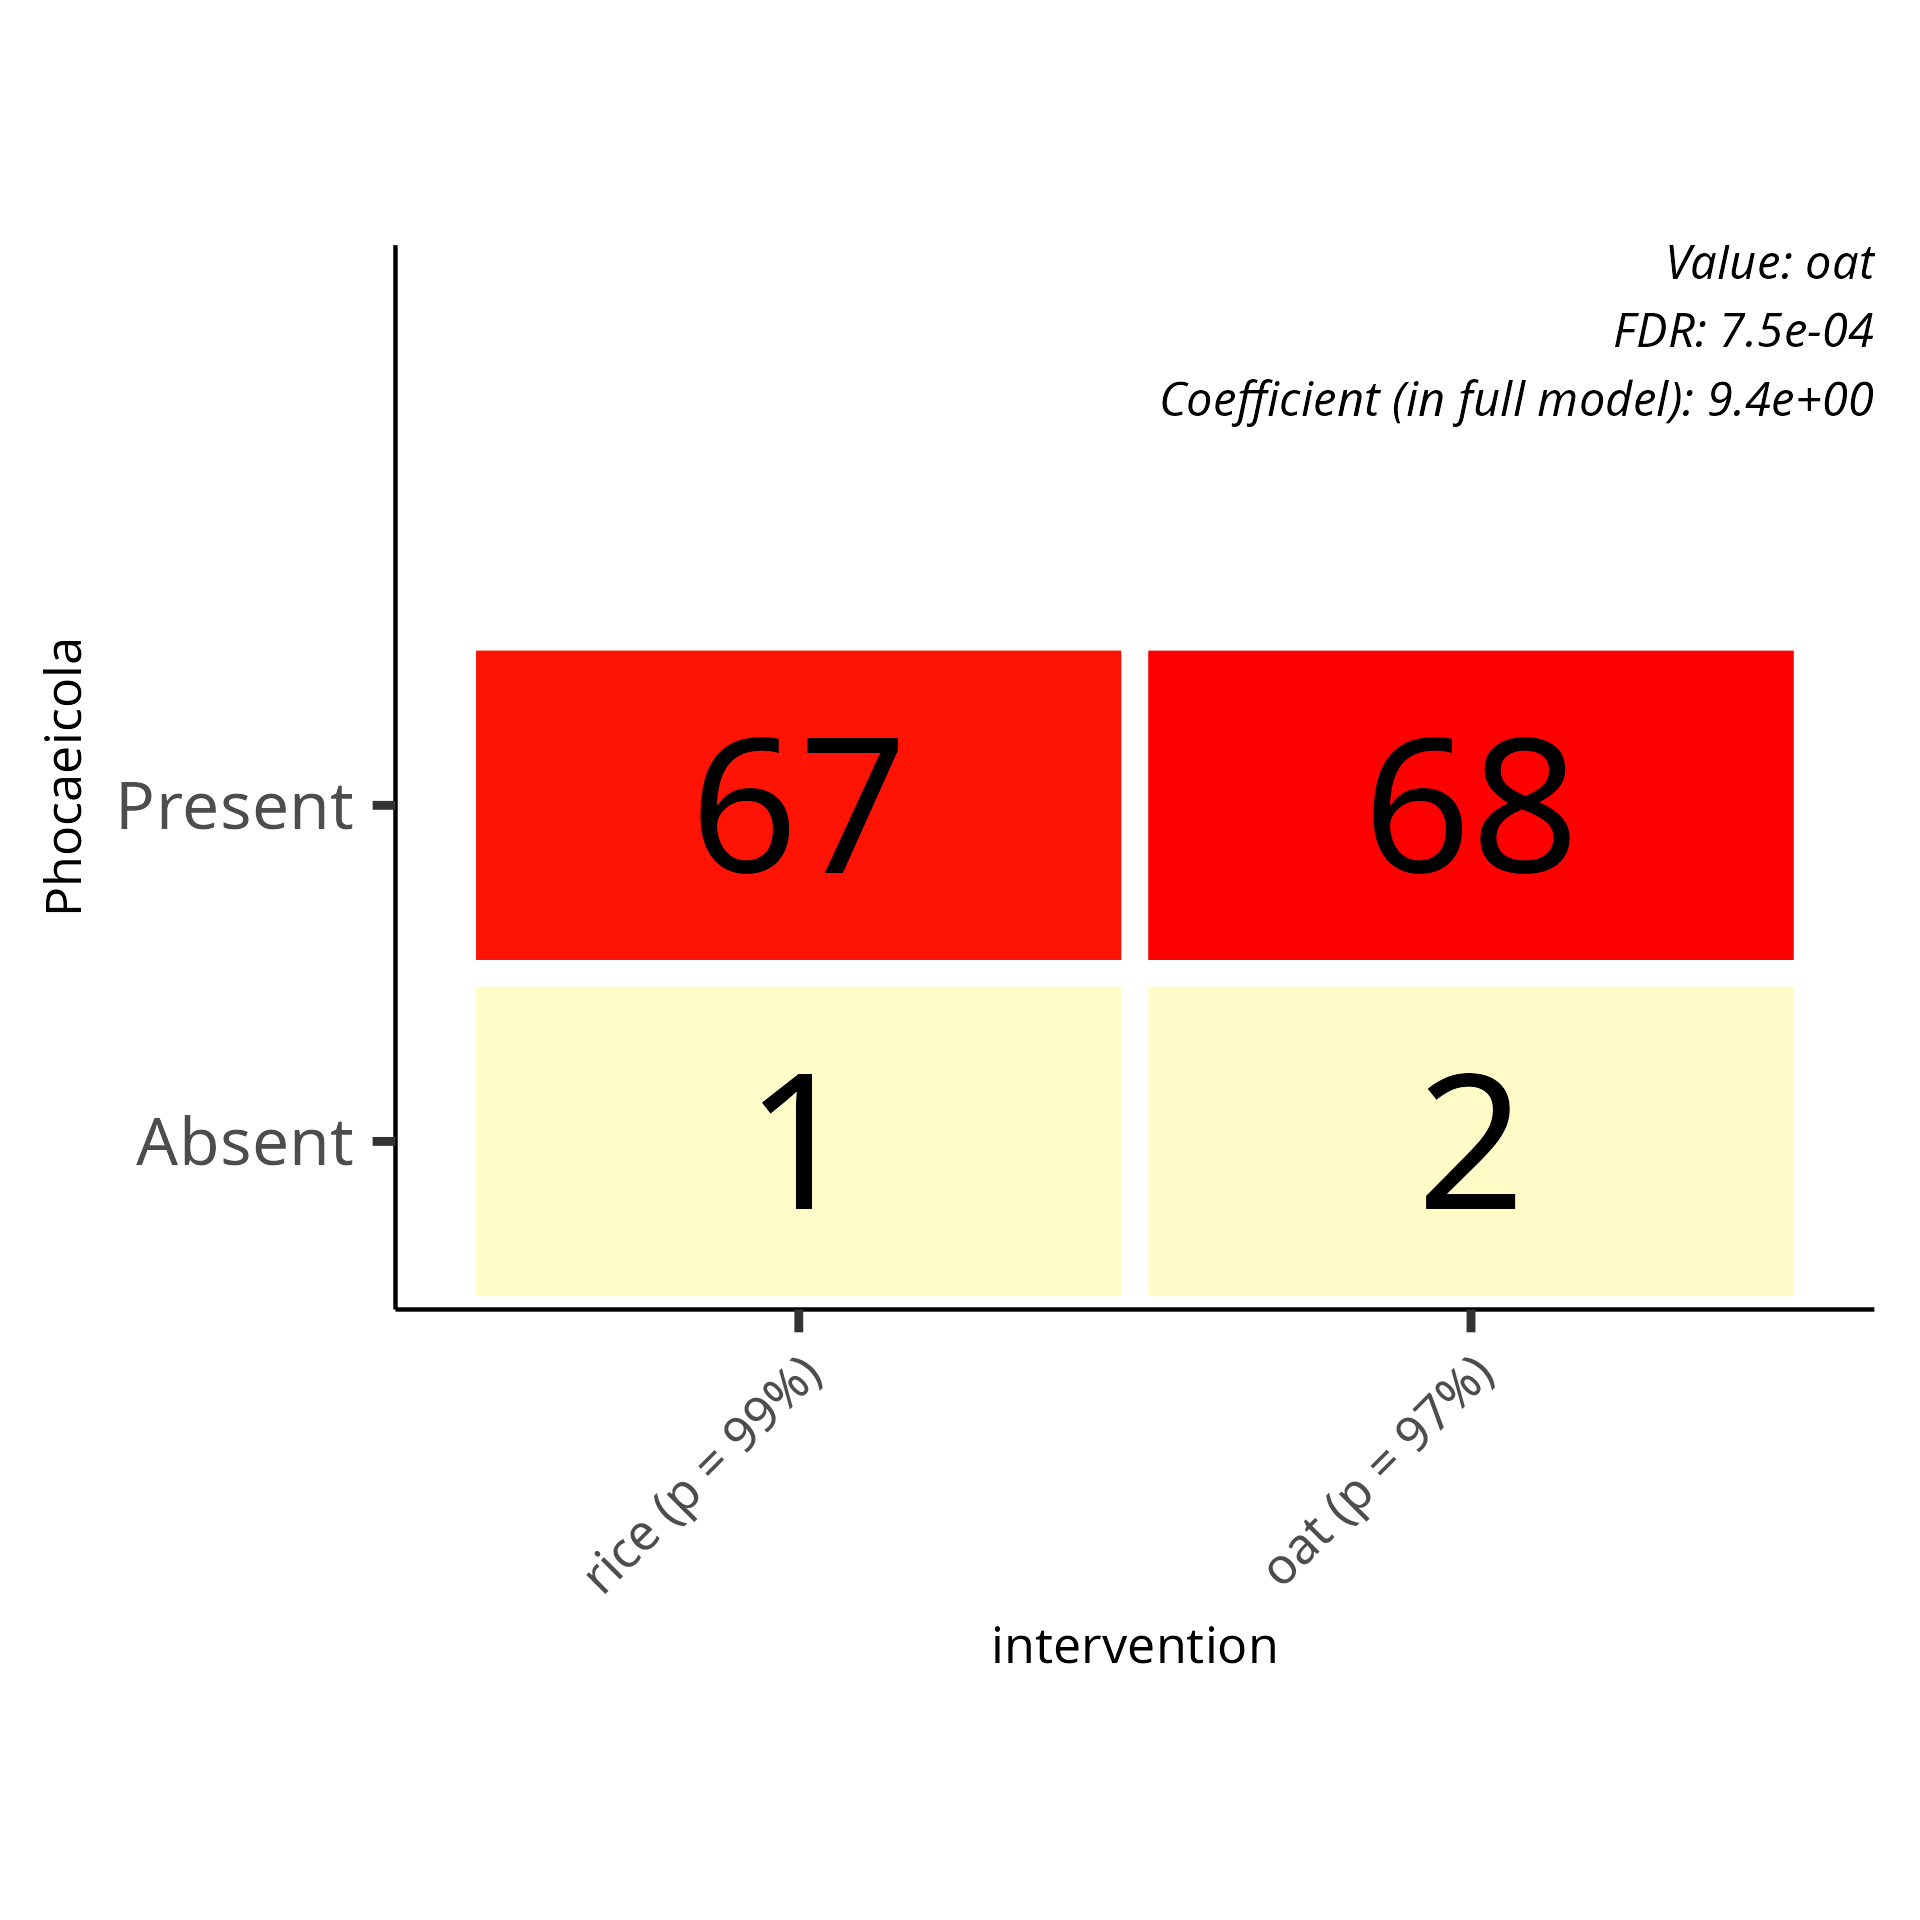
\includegraphics{../../output/daa/daa_taxa/genus/figures/association_plots/intervention/logistic/intervention_Phocaeicola_logistic.png}\\
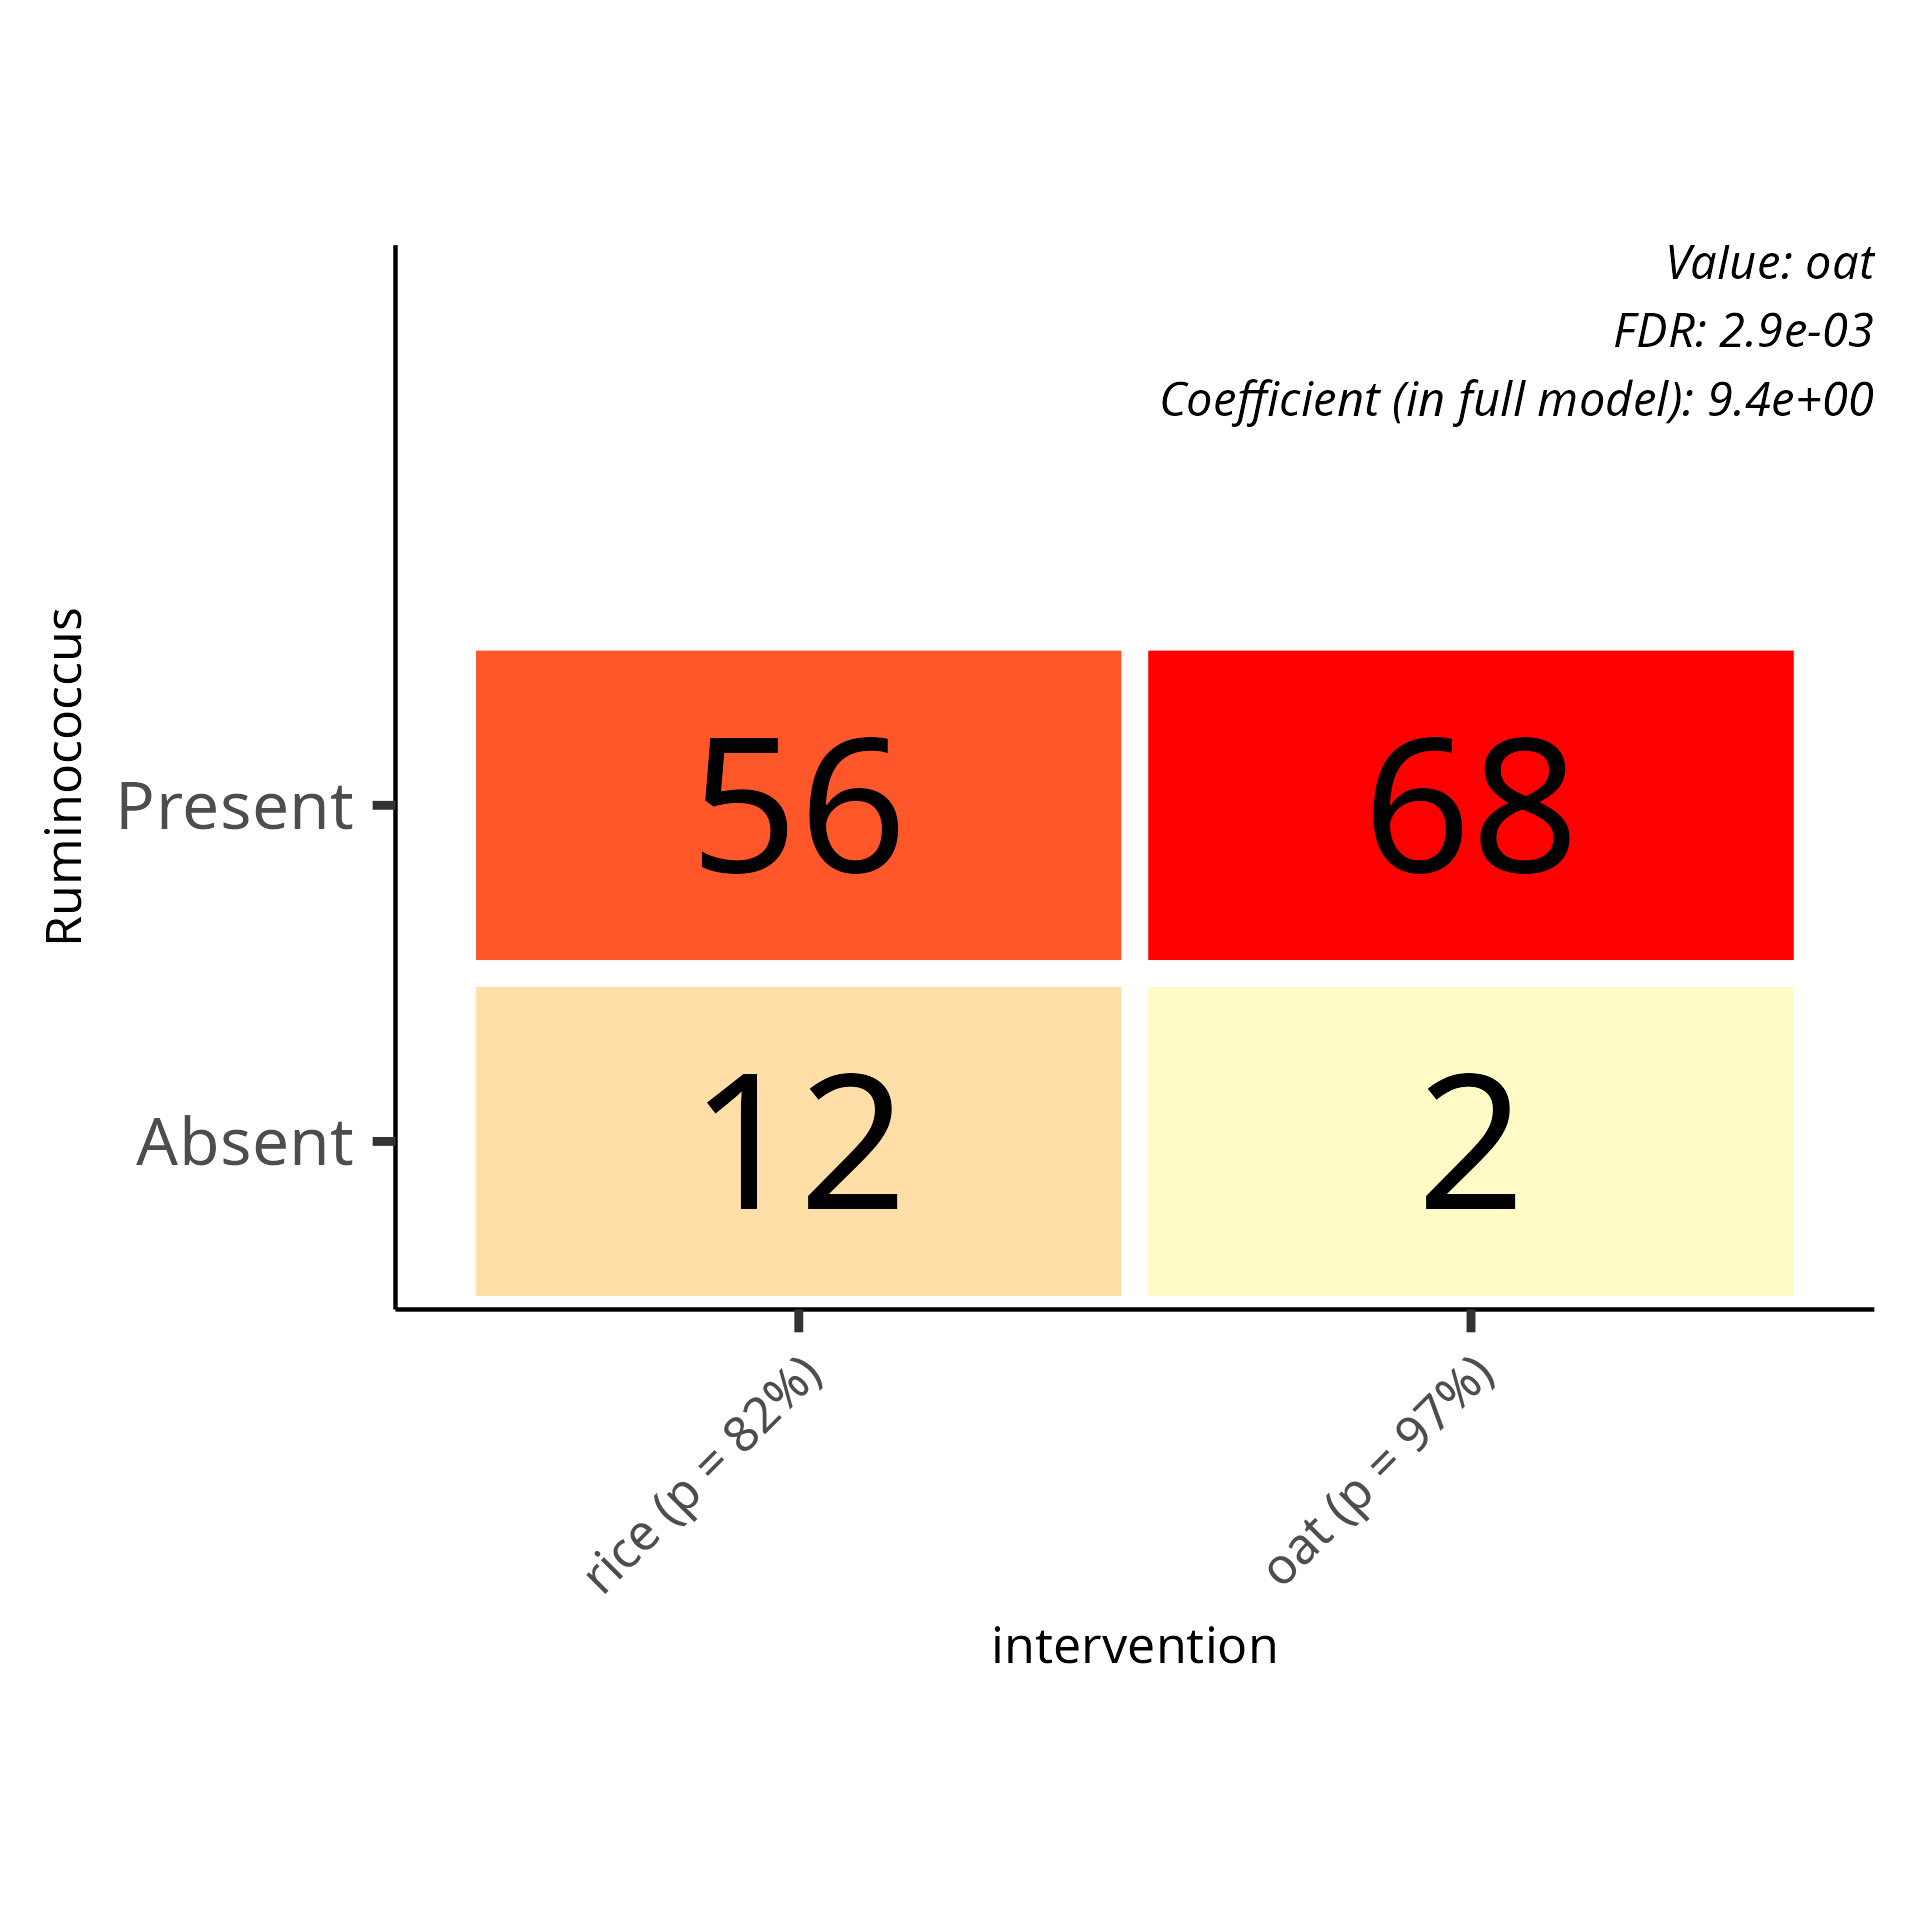
\includegraphics{../../output/daa/daa_taxa/genus/figures/association_plots/intervention/logistic/intervention_Ruminococcus_logistic.png}




\end{document}
